\clearpage
\subsection{\texttt{1p2d\_M1.7\_eth}}\label{net:1p2d_M1.7_eth}
\noindent\begin{minipage}[t]{0.43\textwidth}\vspace{0pt}\footnotesize
\begin{tabular}{@{}rrlrr@{}}
\toprule
id & gen & $(\ell,n)$ & $\omega$ [rad\,s$^{-1}$] & $\gamma$ [s$^{-1}$] \\
\midrule
0 & 0 & (1,+1) & $1.402\times10^{-3}$ & $-1.150\times10^{-10}$ \\
1 & 1 & (6,$-$6) & $1.070\times10^{-3}$ & $4.184\times10^{-13}$ \\
2 & 1 & (7,$-$27) & $3.326\times10^{-4}$ & $8.612\times10^{-10}$ \\
\bottomrule
\end{tabular}
\end{minipage}\hfill
\begin{minipage}[t]{0.55\textwidth}\vspace{0pt}\footnotesize
\textbf{Model} \texttt{dsct\_M1.7\_T7750}, rule eth, $N=1$, cut 0.15,
closure 0.005; 3 modes, 1 triplet(s).\\[2pt]
\textbf{Selecting pairs}\\ (1,+1) $\to$ (6,$-$6) + (7,$-$27): $\Delta/\omega_a=-3.98\times10^{-5}$, $\kappa=+0.107$, $E_{\rm th}=9.22\times10^{-11}$, $E_{\rm eq}=1.23\times10^{-10}$\\[2pt]
The second burst disagreed between rk8pd and BDF in the earlier sweep.
\end{minipage}

\par\smallskip{\centering\begin{tabular}{@{}c@{\hspace{2pt}}c@{\hspace{2pt}}c@{\hspace{2pt}}c@{\hspace{2pt}}c@{}}
 & \small atol $10^{-40}$ & \small atol $10^{-150}$ & \small atol $10^{-300}$ & \small atol $0$ \\[1pt]
\rotatebox{90}{\parbox{0.1323\textwidth}{\centering\scriptsize\bfseries rk8pd}} & 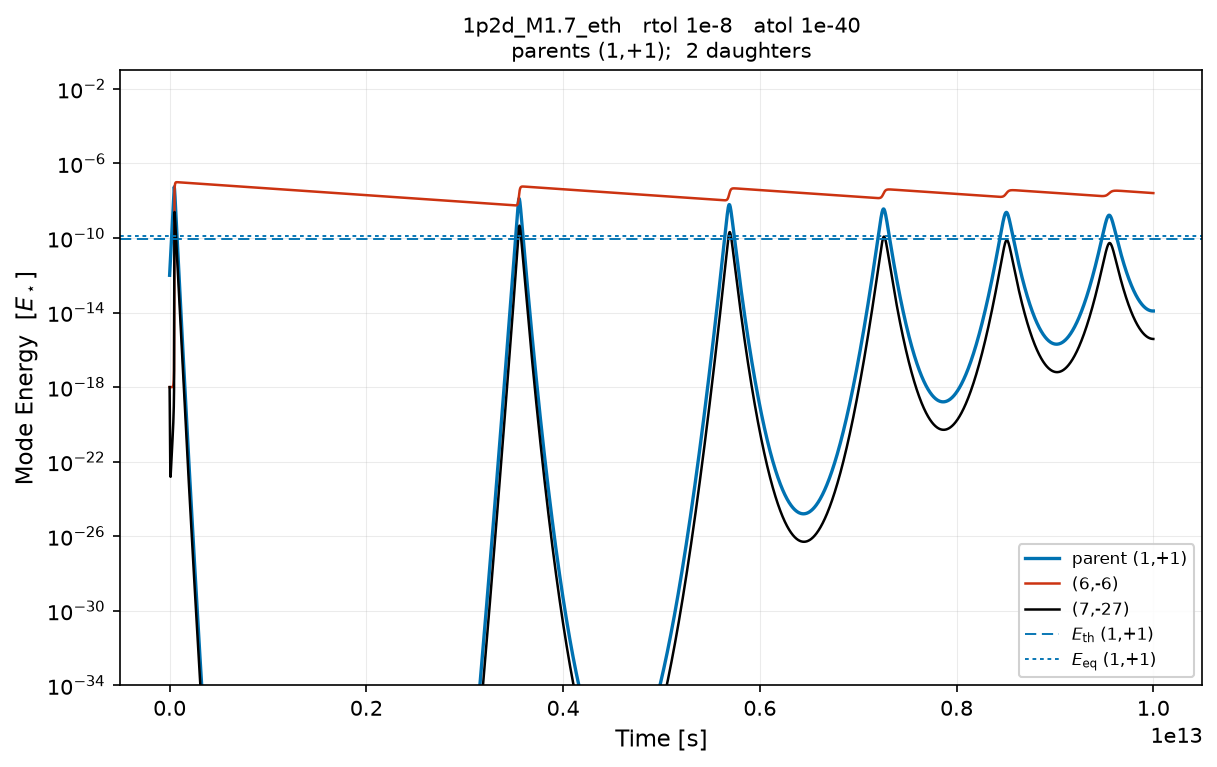
\includegraphics[width=0.21\textwidth,height=0.1323\textwidth]{../plots/rk8pd/1p2d_M1.7_eth/r1e-8_a1e-40.png} & 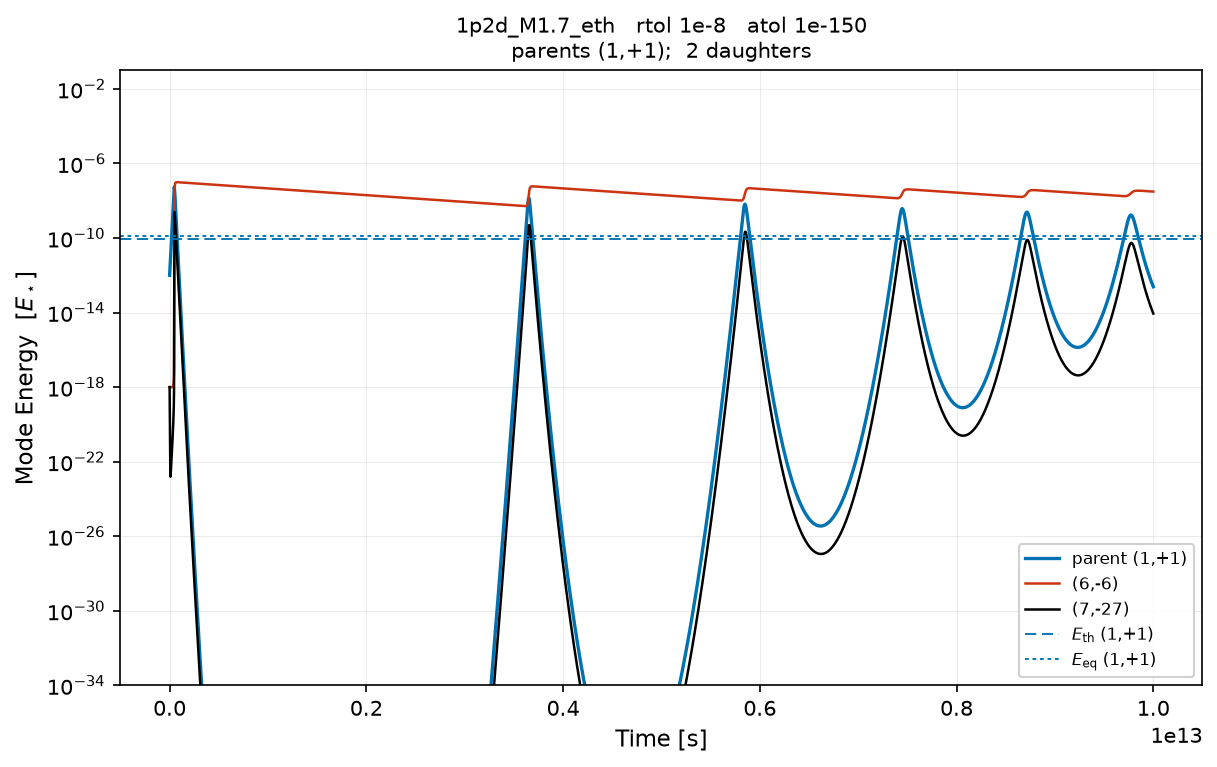
\includegraphics[width=0.21\textwidth,height=0.1323\textwidth]{../plots/rk8pd/1p2d_M1.7_eth/r1e-8_a1e-150.png} & 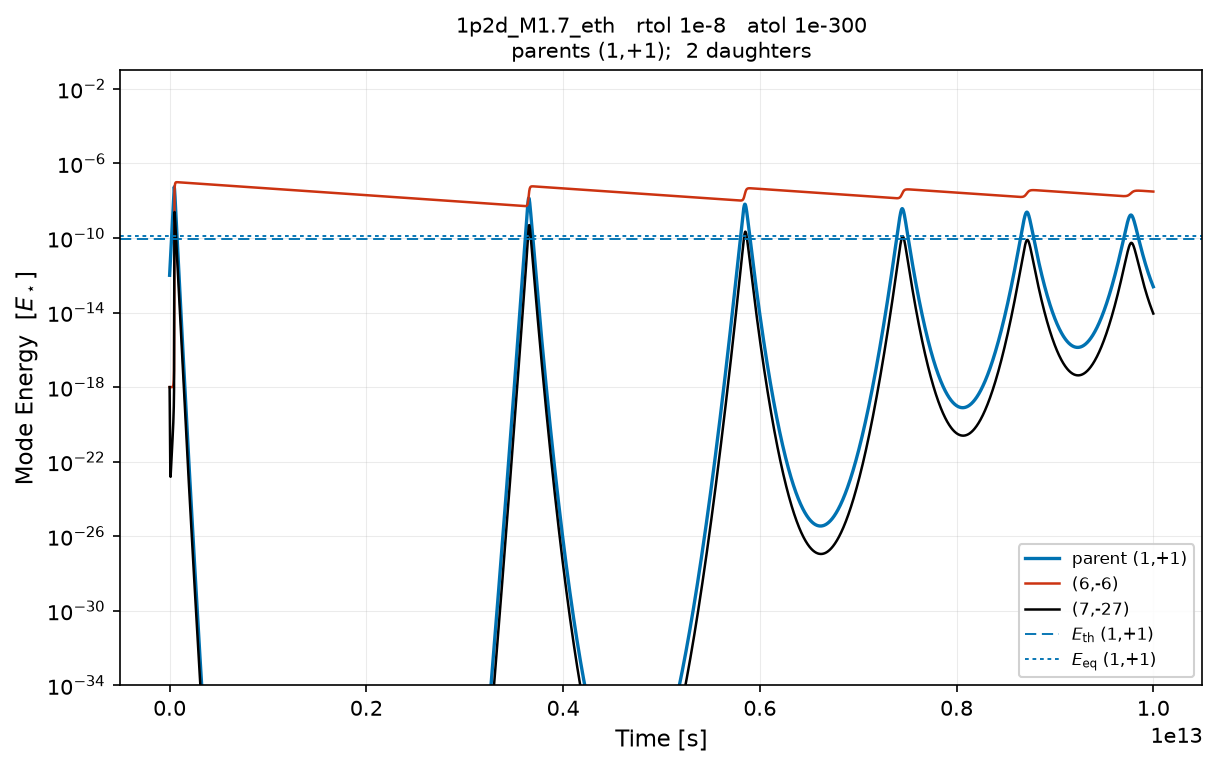
\includegraphics[width=0.21\textwidth,height=0.1323\textwidth]{../plots/rk8pd/1p2d_M1.7_eth/r1e-8_a1e-300.png} & 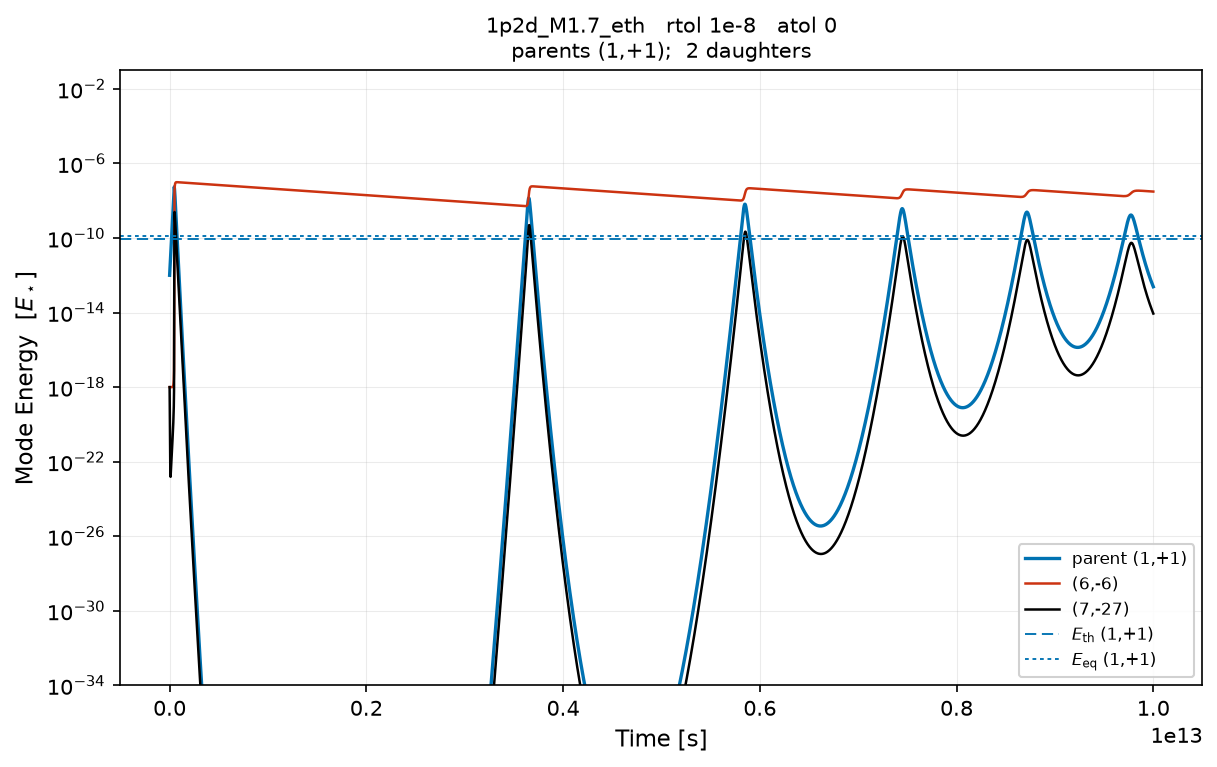
\includegraphics[width=0.21\textwidth,height=0.1323\textwidth]{../plots/rk8pd/1p2d_M1.7_eth/r1e-8_a0.png} \\[-1pt]
 & \parbox[t]{0.21\textwidth}{\centering\scriptsize 953.2\,k steps, 1.5\,s} & \parbox[t]{0.21\textwidth}{\centering\scriptsize 1.13\,M steps, 2.3\,s} & \parbox[t]{0.21\textwidth}{\centering\scriptsize 1.13\,M steps, 2.2\,s} & \parbox[t]{0.21\textwidth}{\centering\scriptsize 1.13\,M steps, 2.8\,s} \\[2pt]
\rotatebox{90}{\parbox{0.1323\textwidth}{\centering\scriptsize\bfseries BDF, dense analytic Jacobian}} & 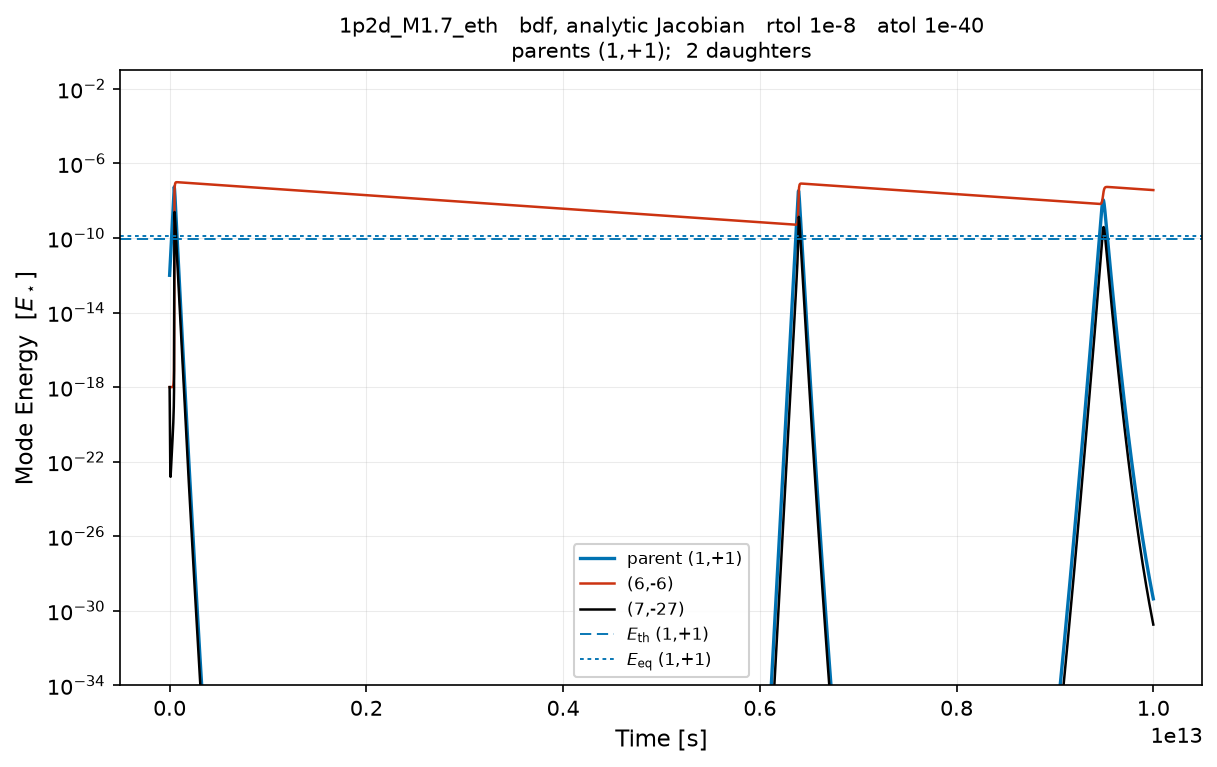
\includegraphics[width=0.21\textwidth,height=0.1323\textwidth]{../plots/bdf/1p2d_M1.7_eth/r1e-8_a1e-40.png} & 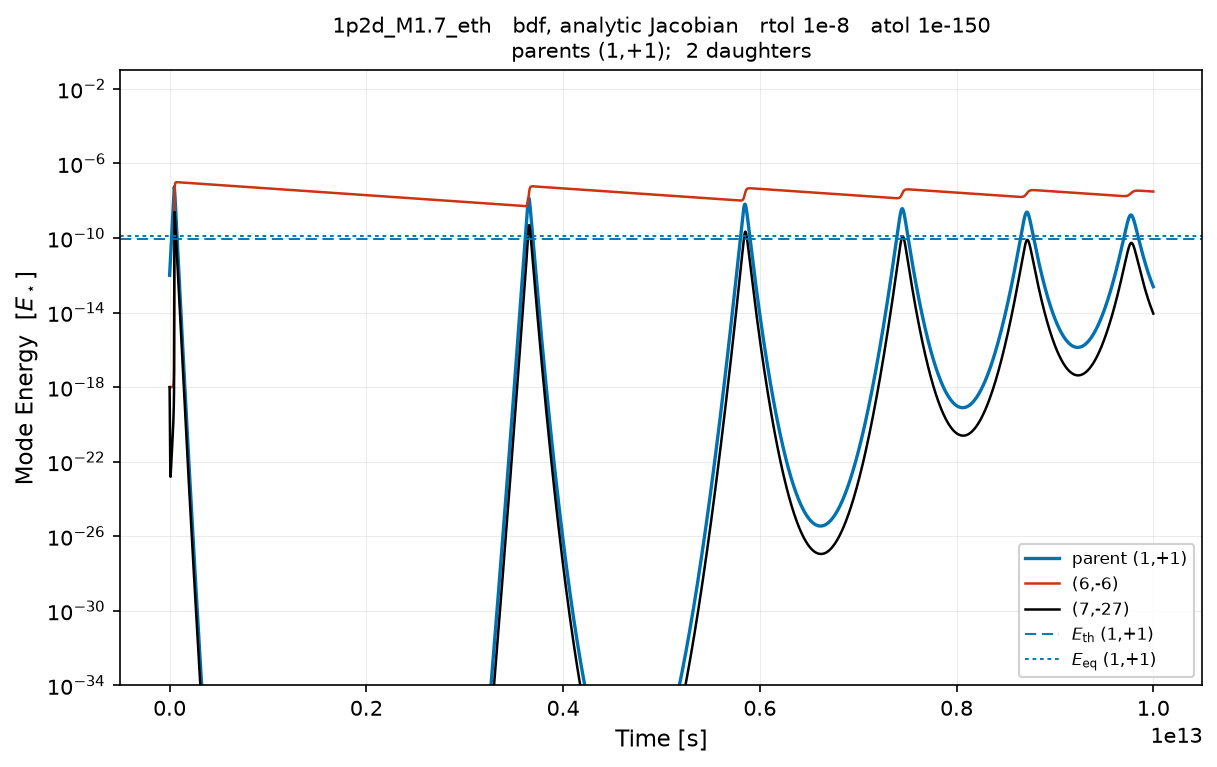
\includegraphics[width=0.21\textwidth,height=0.1323\textwidth]{../plots/bdf/1p2d_M1.7_eth/r1e-8_a1e-150.png} & 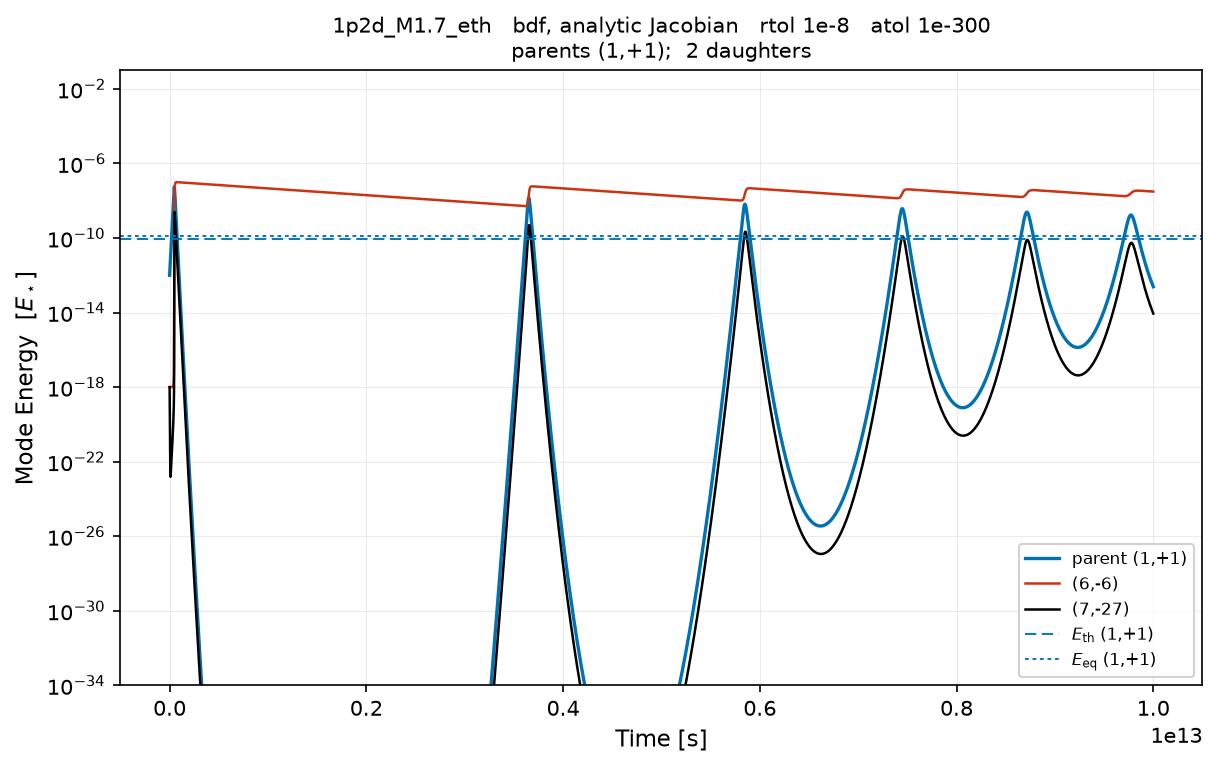
\includegraphics[width=0.21\textwidth,height=0.1323\textwidth]{../plots/bdf/1p2d_M1.7_eth/r1e-8_a1e-300.png} & 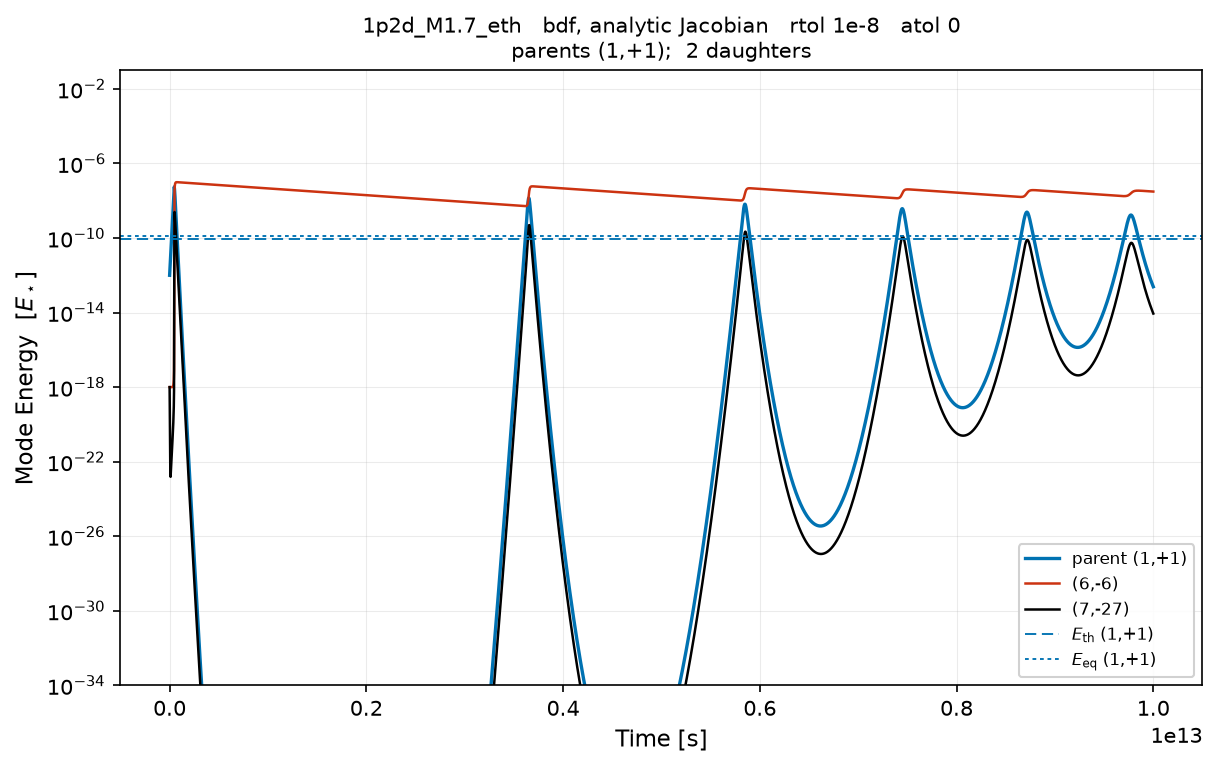
\includegraphics[width=0.21\textwidth,height=0.1323\textwidth]{../plots/bdf/1p2d_M1.7_eth/r1e-8_a0.png} \\[-1pt]
 & \parbox[t]{0.21\textwidth}{\centering\scriptsize 6.39\,M steps, 5.7\,s} & \parbox[t]{0.21\textwidth}{\centering\scriptsize 13.78\,M steps, 14.5\,s} & \parbox[t]{0.21\textwidth}{\centering\scriptsize 13.78\,M steps, 10.2\,s} & \parbox[t]{0.21\textwidth}{\centering\scriptsize 13.78\,M steps, 16.3\,s} \\[2pt]
\rotatebox{90}{\parbox{0.1323\textwidth}{\centering\scriptsize\bfseries BDF-Krylov, band full}} & 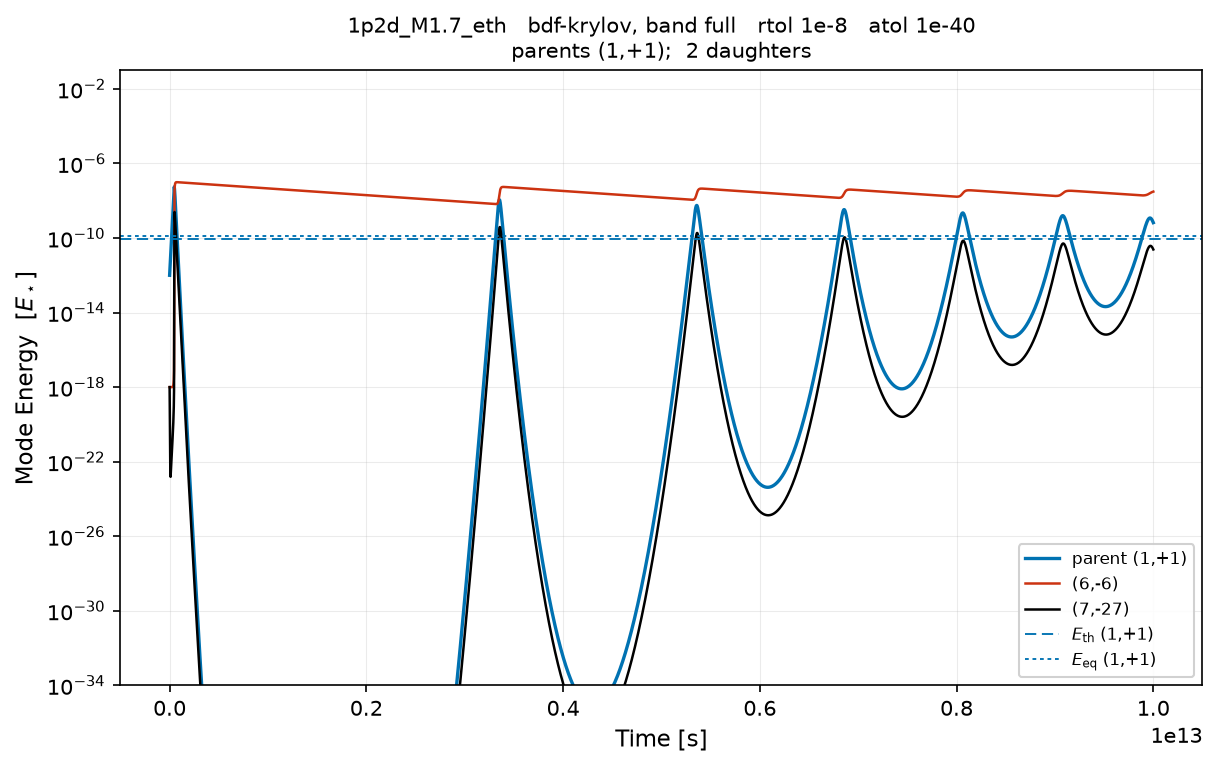
\includegraphics[width=0.21\textwidth,height=0.1323\textwidth]{../plots/krylov_full/1p2d_M1.7_eth/r1e-8_a1e-40.png} & 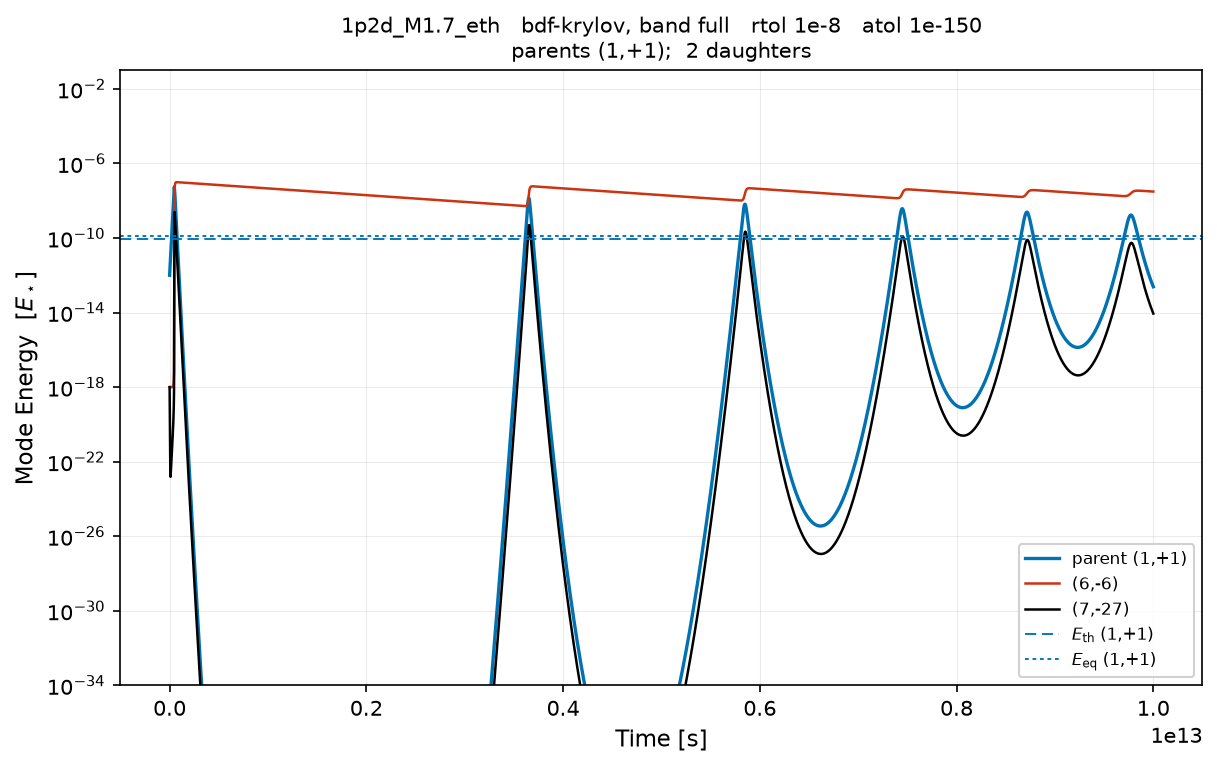
\includegraphics[width=0.21\textwidth,height=0.1323\textwidth]{../plots/krylov_full/1p2d_M1.7_eth/r1e-8_a1e-150.png} & 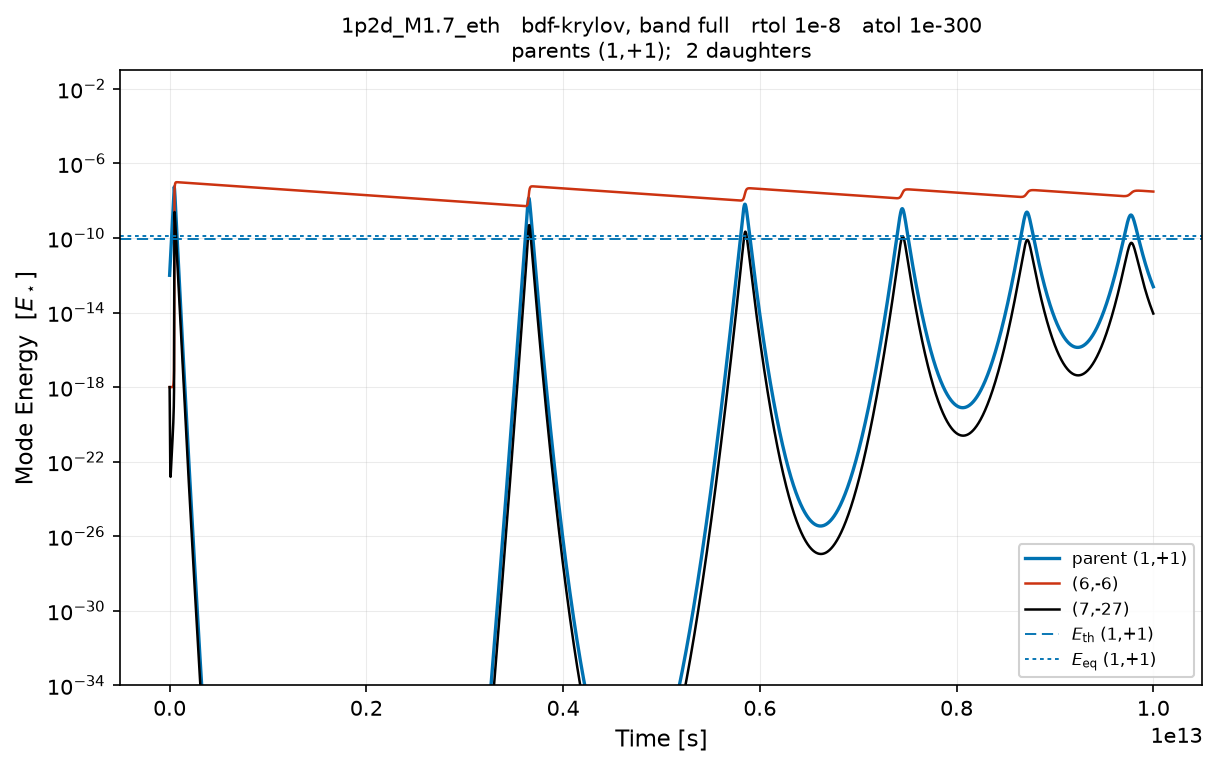
\includegraphics[width=0.21\textwidth,height=0.1323\textwidth]{../plots/krylov_full/1p2d_M1.7_eth/r1e-8_a1e-300.png} & 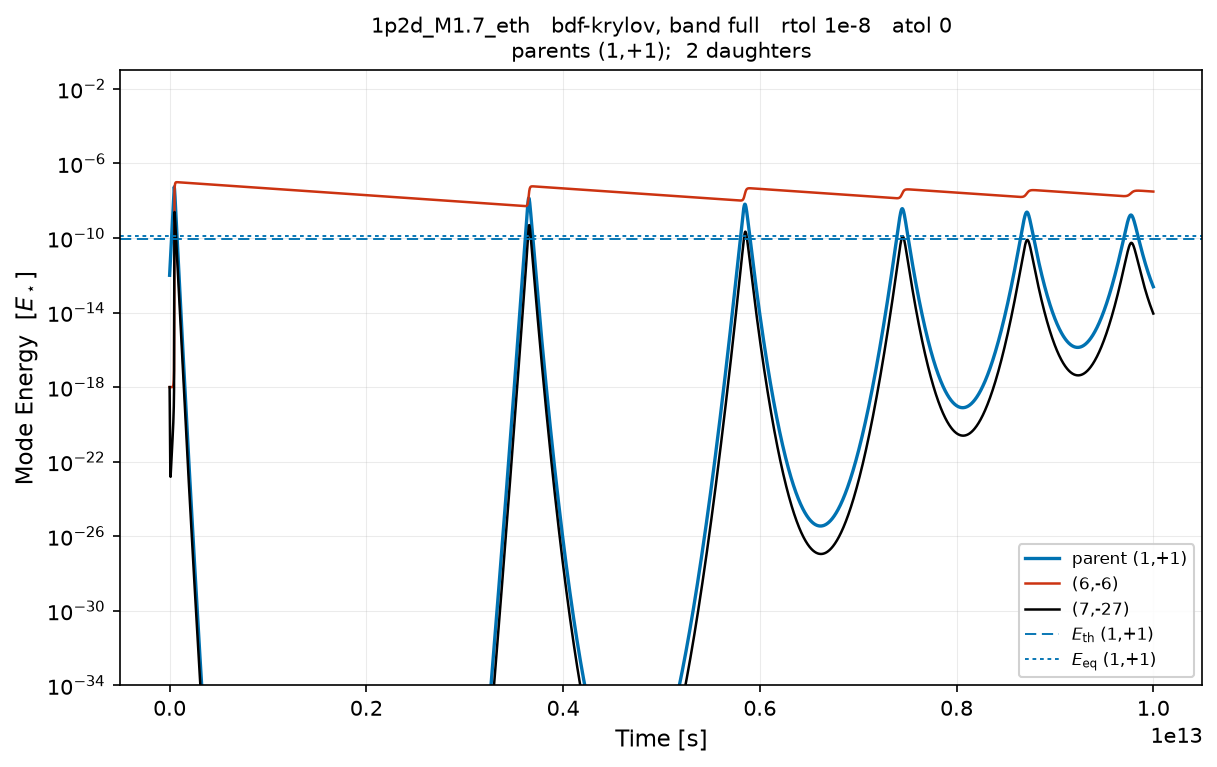
\includegraphics[width=0.21\textwidth,height=0.1323\textwidth]{../plots/krylov_full/1p2d_M1.7_eth/r1e-8_a0.png} \\[-1pt]
 & \parbox[t]{0.21\textwidth}{\centering\scriptsize 12.00\,M steps, 22.8\,s} & \parbox[t]{0.21\textwidth}{\centering\scriptsize 13.44\,M steps, 25.5\,s} & \parbox[t]{0.21\textwidth}{\centering\scriptsize 13.44\,M steps, 17.4\,s} & \parbox[t]{0.21\textwidth}{\centering\scriptsize 13.44\,M steps, 16.8\,s} \\[2pt]
\rotatebox{90}{\parbox{0.1323\textwidth}{\centering\scriptsize\bfseries BDF-Krylov, band 3}} & 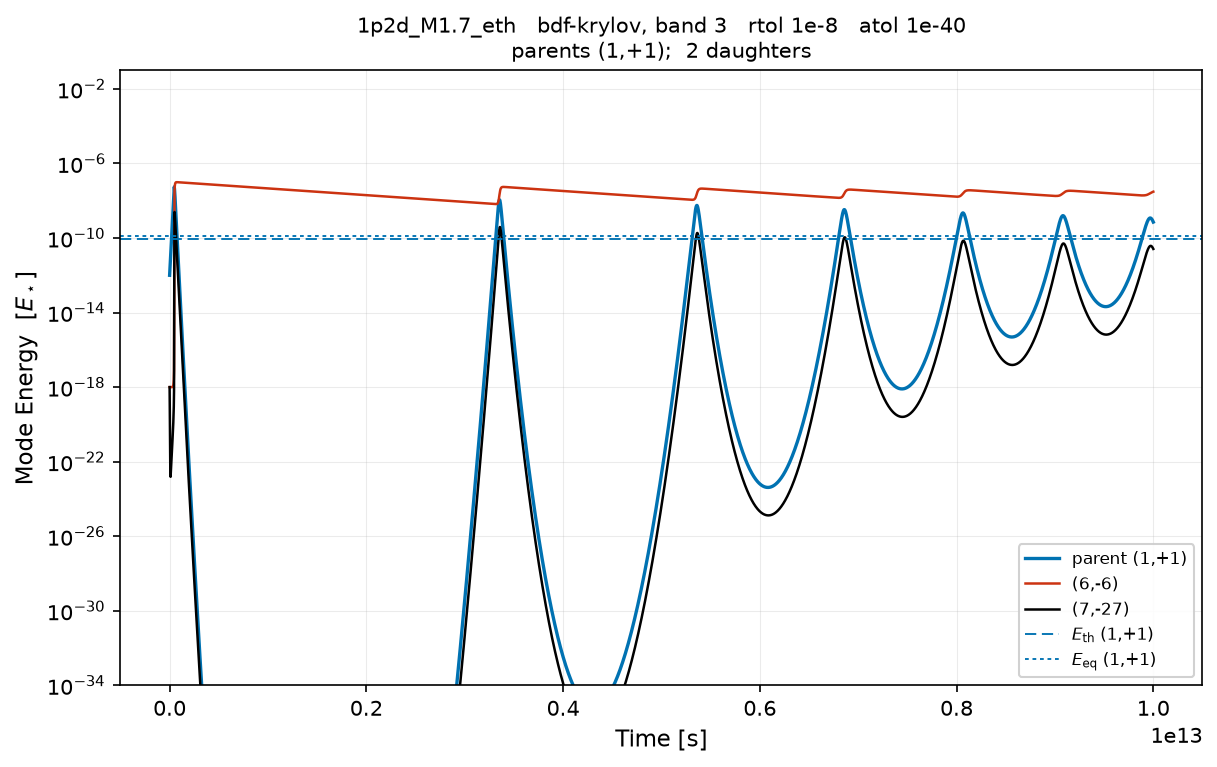
\includegraphics[width=0.21\textwidth,height=0.1323\textwidth]{../plots/krylov_b3/1p2d_M1.7_eth/r1e-8_a1e-40.png} & 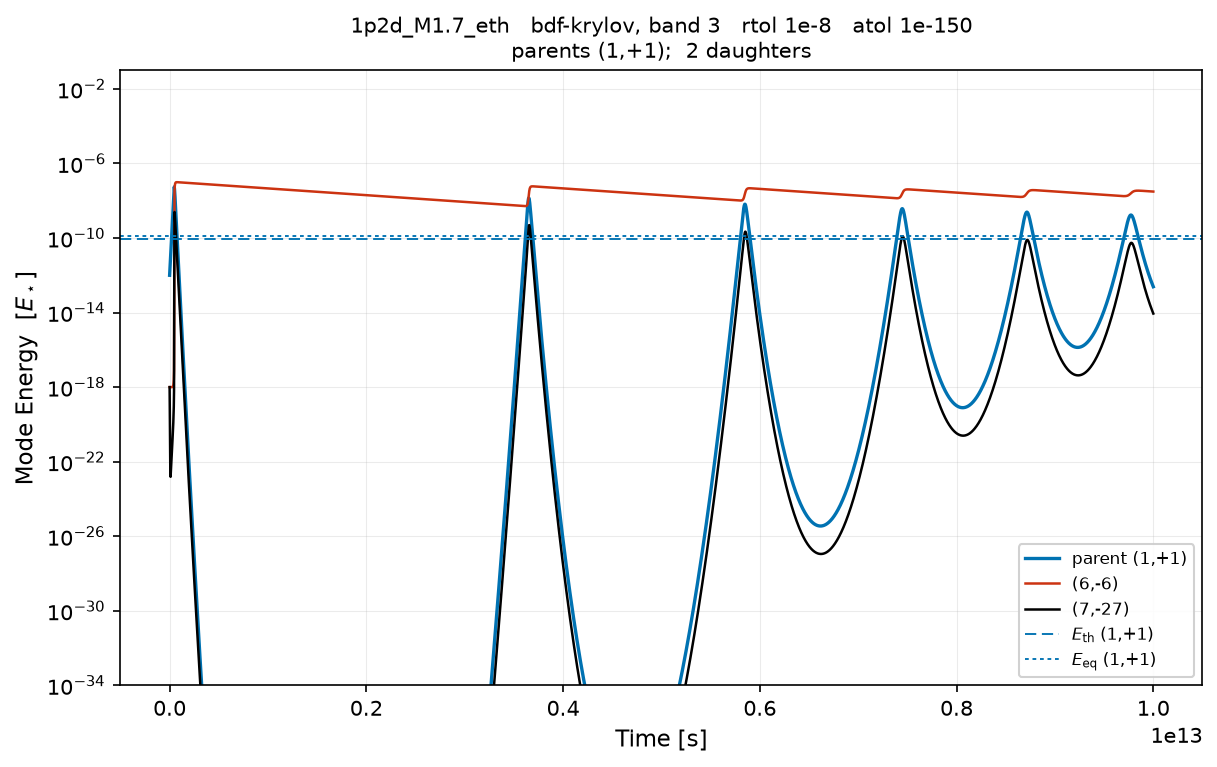
\includegraphics[width=0.21\textwidth,height=0.1323\textwidth]{../plots/krylov_b3/1p2d_M1.7_eth/r1e-8_a1e-150.png} & 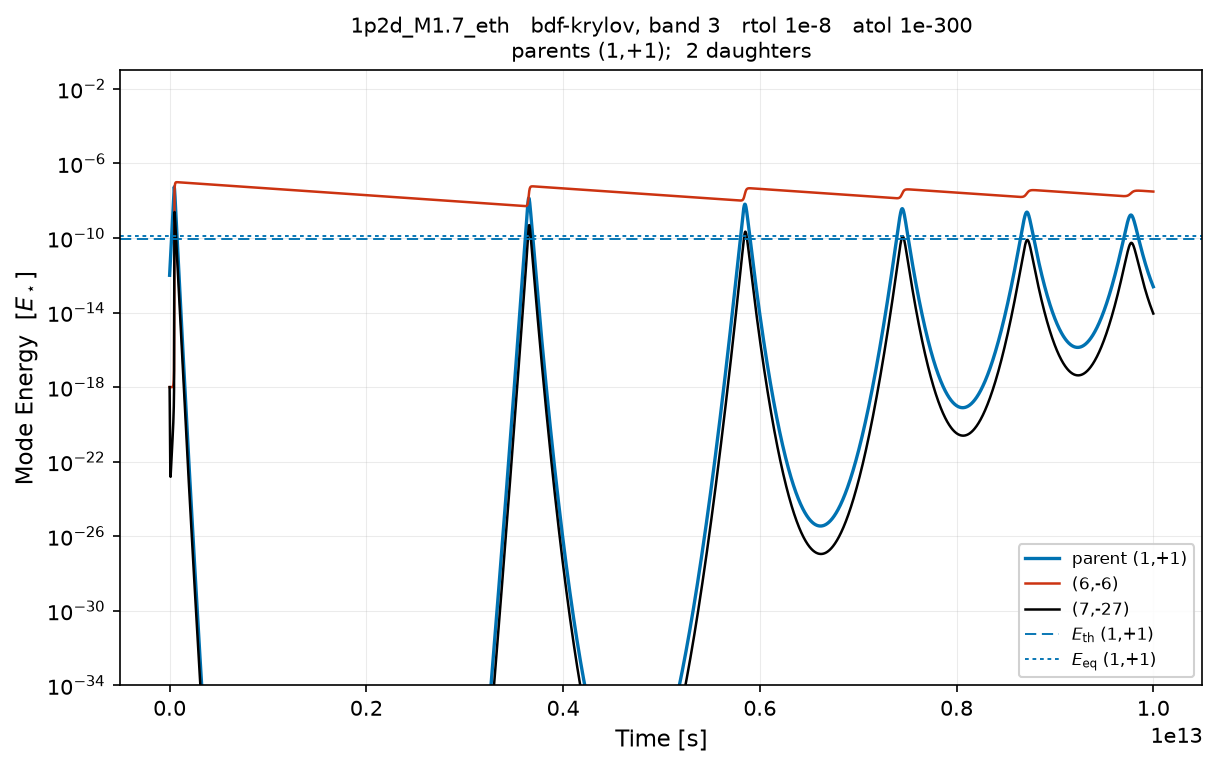
\includegraphics[width=0.21\textwidth,height=0.1323\textwidth]{../plots/krylov_b3/1p2d_M1.7_eth/r1e-8_a1e-300.png} & 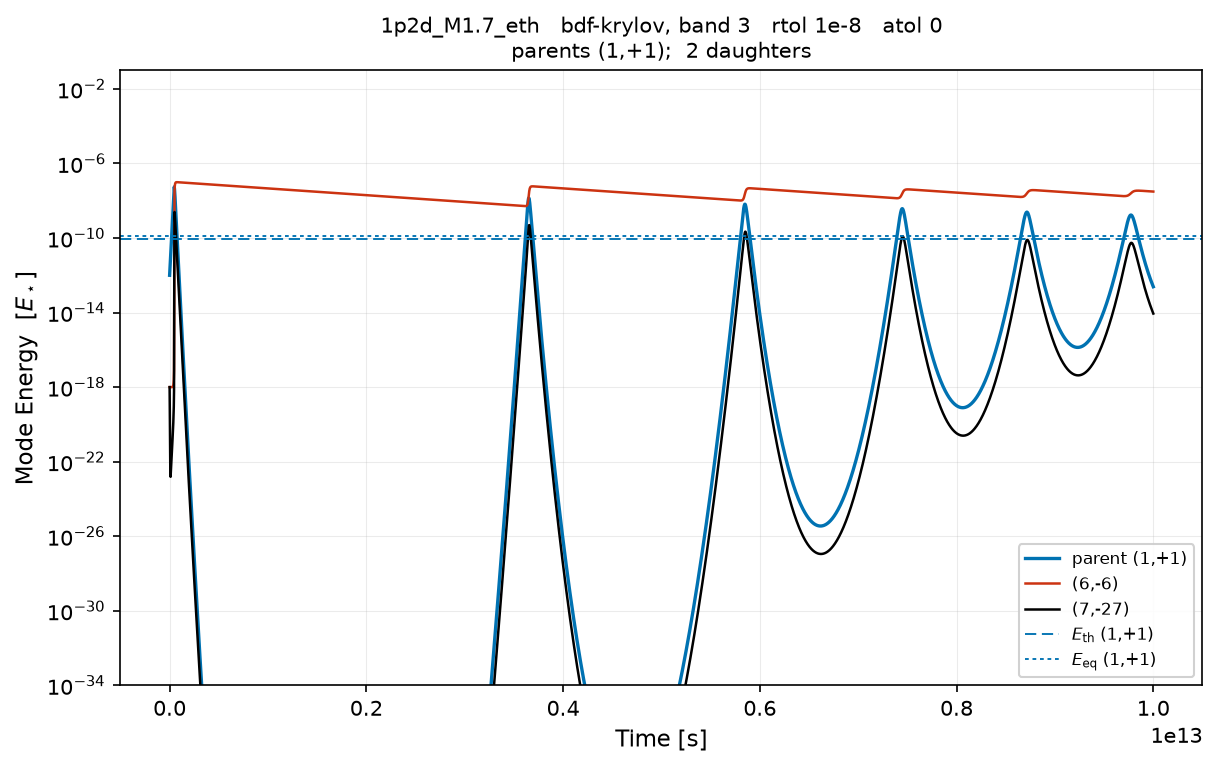
\includegraphics[width=0.21\textwidth,height=0.1323\textwidth]{../plots/krylov_b3/1p2d_M1.7_eth/r1e-8_a0.png} \\[-1pt]
 & \parbox[t]{0.21\textwidth}{\centering\scriptsize 11.86\,M steps, 16.6\,s} & \parbox[t]{0.21\textwidth}{\centering\scriptsize 13.28\,M steps, 20.7\,s} & \parbox[t]{0.21\textwidth}{\centering\scriptsize 13.28\,M steps, 25.0\,s} & \parbox[t]{0.21\textwidth}{\centering\scriptsize 13.28\,M steps, 14.9\,s} \\[2pt]
\rotatebox{90}{\parbox{0.1323\textwidth}{\centering\scriptsize\bfseries Adams, fixed point}} & 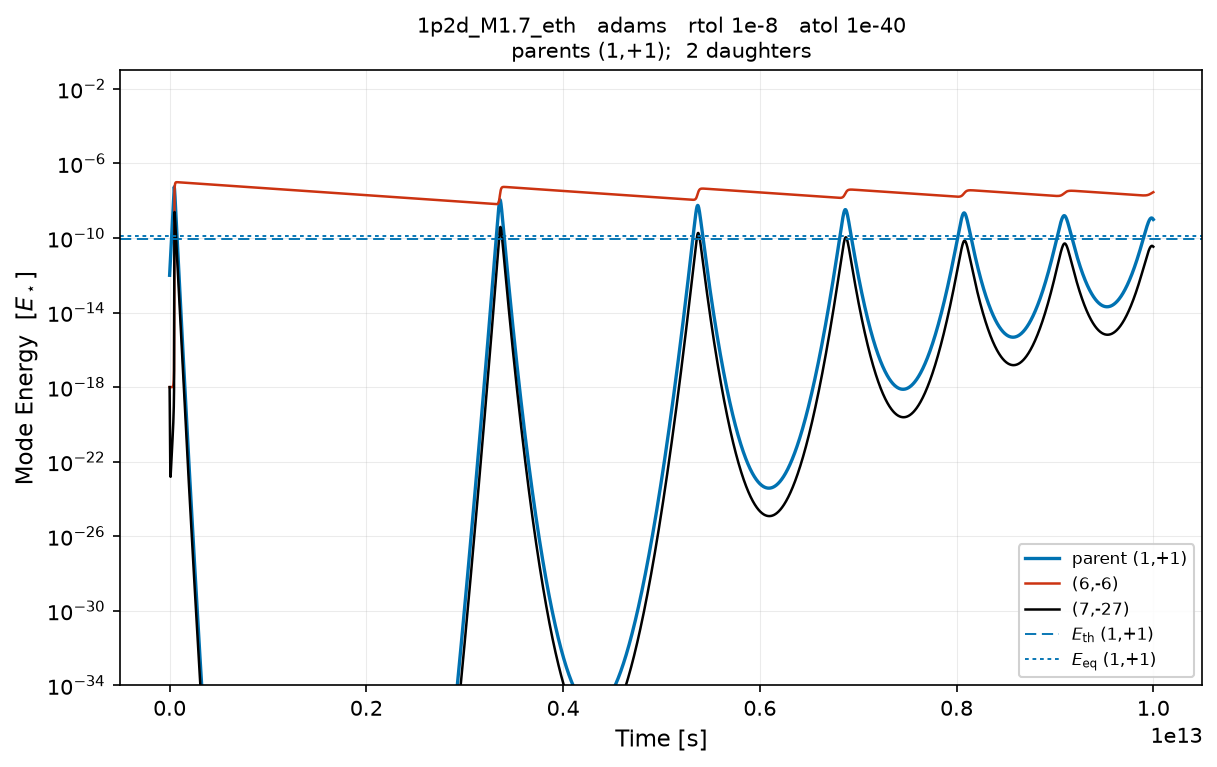
\includegraphics[width=0.21\textwidth,height=0.1323\textwidth]{../plots/adams/1p2d_M1.7_eth/r1e-8_a1e-40.png} & 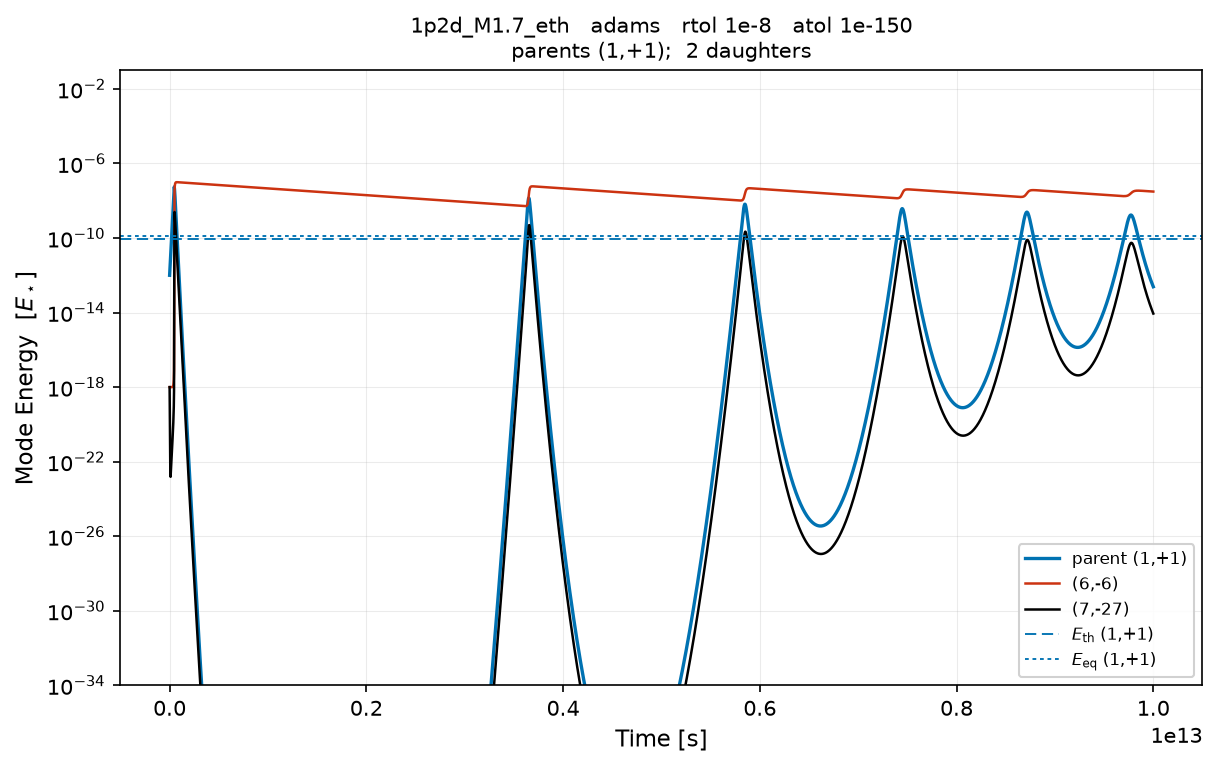
\includegraphics[width=0.21\textwidth,height=0.1323\textwidth]{../plots/adams/1p2d_M1.7_eth/r1e-8_a1e-150.png} & 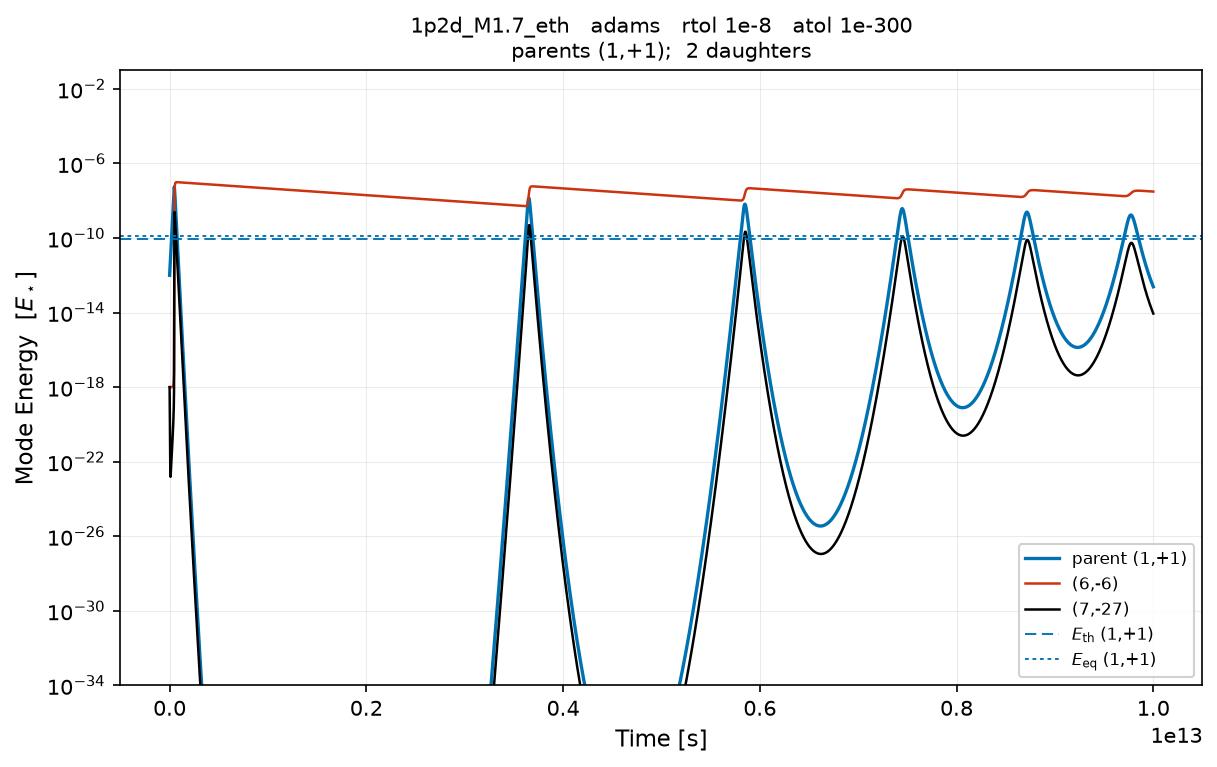
\includegraphics[width=0.21\textwidth,height=0.1323\textwidth]{../plots/adams/1p2d_M1.7_eth/r1e-8_a1e-300.png} & 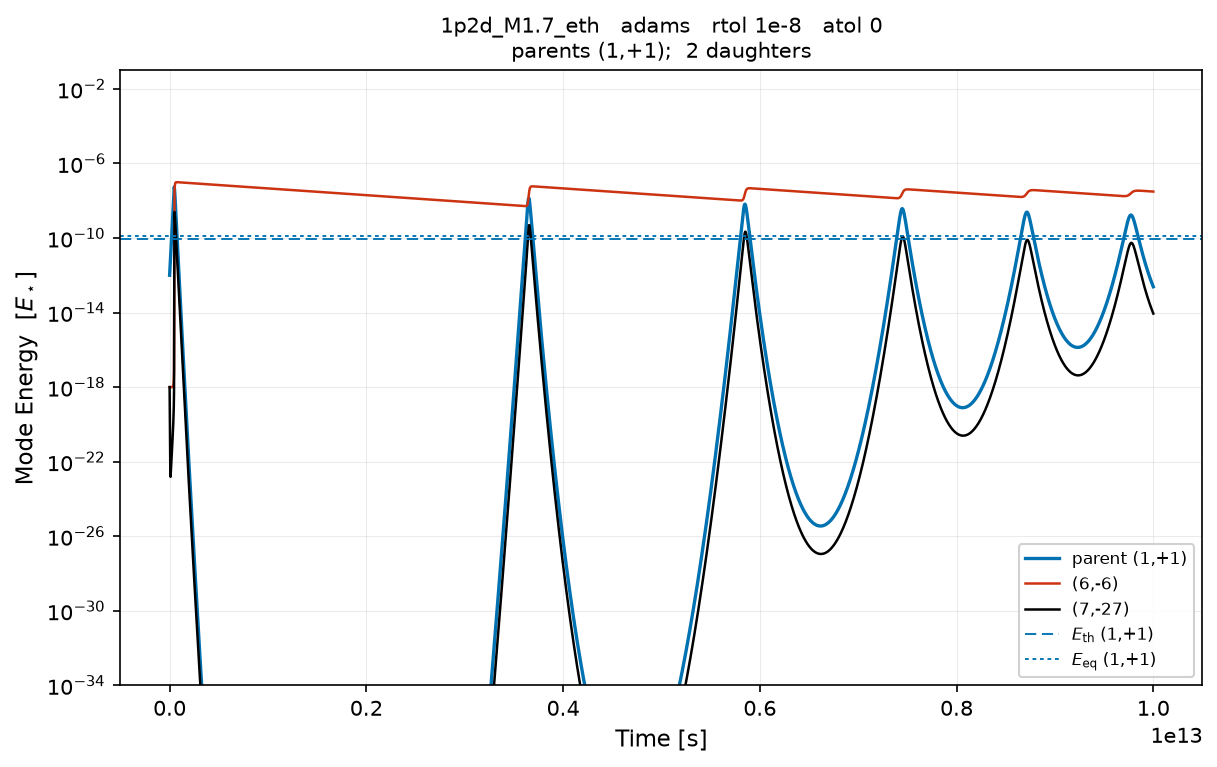
\includegraphics[width=0.21\textwidth,height=0.1323\textwidth]{../plots/adams/1p2d_M1.7_eth/r1e-8_a0.png} \\[-1pt]
 & \parbox[t]{0.21\textwidth}{\centering\scriptsize 5.47\,M steps, 7.2\,s} & \parbox[t]{0.21\textwidth}{\centering\scriptsize 5.88\,M steps, 8.0\,s} & \parbox[t]{0.21\textwidth}{\centering\scriptsize 5.88\,M steps, 8.0\,s} & \parbox[t]{0.21\textwidth}{\centering\scriptsize 5.88\,M steps, 8.0\,s} \\[2pt]
\end{tabular}\par}
\par\noindent{\scriptsize\setlength\tabcolsep{3.5pt}\renewcommand\arraystretch{0.92}
\begin{tabular}{@{}llllrrrrrrr@{}}
\toprule
integrator & atol & stop & $t_{\rm stop}$ [s] & steps & rejected & RHS & Jac. & NL it. & lin. it. & wall [s] \\
\midrule
rk8pd & $10^{-40}$ & end & $1.00\times10^{13}$ & 953.2\,k & 101.3\,k & 12.39\,M & -- & -- & -- & 1.5 \\
 & $10^{-150}$ & end & $1.00\times10^{13}$ & 1.13\,M & 126.8\,k & 14.65\,M & -- & -- & -- & 2.3 \\
 & $10^{-300}$ & end & $1.00\times10^{13}$ & 1.13\,M & 126.8\,k & 14.65\,M & -- & -- & -- & 2.2 \\
 & $0$ & end & $1.00\times10^{13}$ & 1.13\,M & 126.8\,k & 14.65\,M & -- & -- & -- & 2.8 \\
\addlinespace[2pt]
BDF, dense analytic Jacobian & $10^{-40}$ & end & $1.00\times10^{13}$ & 6.39\,M & 49.0\,k & 6.85\,M & 117.8\,k & 6.85\,M & -- & 5.7 \\
 & $10^{-150}$ & end & $1.00\times10^{13}$ & 13.78\,M & 118.0\,k & 14.74\,M & 241.1\,k & 14.74\,M & -- & 14.5 \\
 & $10^{-300}$ & end & $1.00\times10^{13}$ & 13.78\,M & 118.0\,k & 14.74\,M & 241.1\,k & 14.74\,M & -- & 10.2 \\
 & $0$ & end & $1.00\times10^{13}$ & 13.78\,M & 118.0\,k & 14.74\,M & 241.1\,k & 14.74\,M & -- & 16.3 \\
\addlinespace[2pt]
BDF-Krylov, band full & $10^{-40}$ & end & $1.00\times10^{13}$ & 12.00\,M & 104.9\,k & 27.04\,M & 209.5\,k & 12.90\,M & 12.88\,M & 22.8 \\
 & $10^{-150}$ & end & $1.00\times10^{13}$ & 13.44\,M & 125.8\,k & 29.86\,M & 234.6\,k & 14.47\,M & 13.98\,M & 25.5 \\
 & $10^{-300}$ & end & $1.00\times10^{13}$ & 13.44\,M & 125.8\,k & 29.86\,M & 234.6\,k & 14.47\,M & 13.98\,M & 17.4 \\
 & $0$ & end & $1.00\times10^{13}$ & 13.44\,M & 125.8\,k & 29.86\,M & 234.6\,k & 14.47\,M & 13.98\,M & 16.8 \\
\addlinespace[2pt]
BDF-Krylov, band 3 & $10^{-40}$ & end & $1.00\times10^{13}$ & 11.86\,M & 110.2\,k & 26.98\,M & 207.1\,k & 12.80\,M & 12.94\,M & 16.6 \\
 & $10^{-150}$ & end & $1.00\times10^{13}$ & 13.28\,M & 132.1\,k & 29.80\,M & 231.8\,k & 14.35\,M & 14.05\,M & 20.7 \\
 & $10^{-300}$ & end & $1.00\times10^{13}$ & 13.28\,M & 132.1\,k & 29.80\,M & 231.8\,k & 14.35\,M & 14.05\,M & 25.0 \\
 & $0$ & end & $1.00\times10^{13}$ & 13.28\,M & 132.1\,k & 29.80\,M & 231.8\,k & 14.35\,M & 14.05\,M & 14.9 \\
\addlinespace[2pt]
Adams, fixed point & $10^{-40}$ & end & $1.00\times10^{13}$ & 5.47\,M & 231.7\,k & 8.22\,M & -- & 8.22\,M & -- & 7.2 \\
 & $10^{-150}$ & end & $1.00\times10^{13}$ & 5.88\,M & 285.4\,k & 8.57\,M & -- & 8.57\,M & -- & 8.0 \\
 & $10^{-300}$ & end & $1.00\times10^{13}$ & 5.88\,M & 285.4\,k & 8.57\,M & -- & 8.57\,M & -- & 8.0 \\
 & $0$ & end & $1.00\times10^{13}$ & 5.88\,M & 285.4\,k & 8.57\,M & -- & 8.57\,M & -- & 8.0 \\
\bottomrule
\end{tabular}}

\clearpage
\subsection{\texttt{1p2d\_M2.0T\_eth}}\label{net:1p2d_M2.0T_eth}
\noindent\begin{minipage}[t]{0.43\textwidth}\vspace{0pt}\footnotesize
\begin{tabular}{@{}rrlrr@{}}
\toprule
id & gen & $(\ell,n)$ & $\omega$ [rad\,s$^{-1}$] & $\gamma$ [s$^{-1}$] \\
\midrule
0 & 0 & (2,$-$2) & $7.959\times10^{-4}$ & $-6.697\times10^{-11}$ \\
1 & 1 & (3,$-$31) & $1.287\times10^{-4}$ & $8.096\times10^{-11}$ \\
2 & 1 & (5,$-$8) & $6.672\times10^{-4}$ & $7.367\times10^{-13}$ \\
\bottomrule
\end{tabular}
\end{minipage}\hfill
\begin{minipage}[t]{0.55\textwidth}\vspace{0pt}\footnotesize
\textbf{Model} \texttt{dsct\_M2.0\_T7696}, rule eth, $N=1$, cut 0.15,
closure 0.005; 3 modes, 1 triplet(s).\\[2pt]
\textbf{Selecting pairs}\\ (2,$-$2) $\to$ (3,$-$31) + (5,$-$8): $\Delta/\omega_a=-3.69\times10^{-6}$, $\kappa=+0.215$, $E_{\rm th}=4.87\times10^{-12}$, $E_{\rm eq}=1.50\times10^{-10}$\\[2pt]

\end{minipage}

\par\smallskip{\centering\begin{tabular}{@{}c@{\hspace{2pt}}c@{\hspace{2pt}}c@{\hspace{2pt}}c@{\hspace{2pt}}c@{}}
 & \small atol $10^{-40}$ & \small atol $10^{-150}$ & \small atol $10^{-300}$ & \small atol $0$ \\[1pt]
\rotatebox{90}{\parbox{0.1323\textwidth}{\centering\scriptsize\bfseries rk8pd}} & 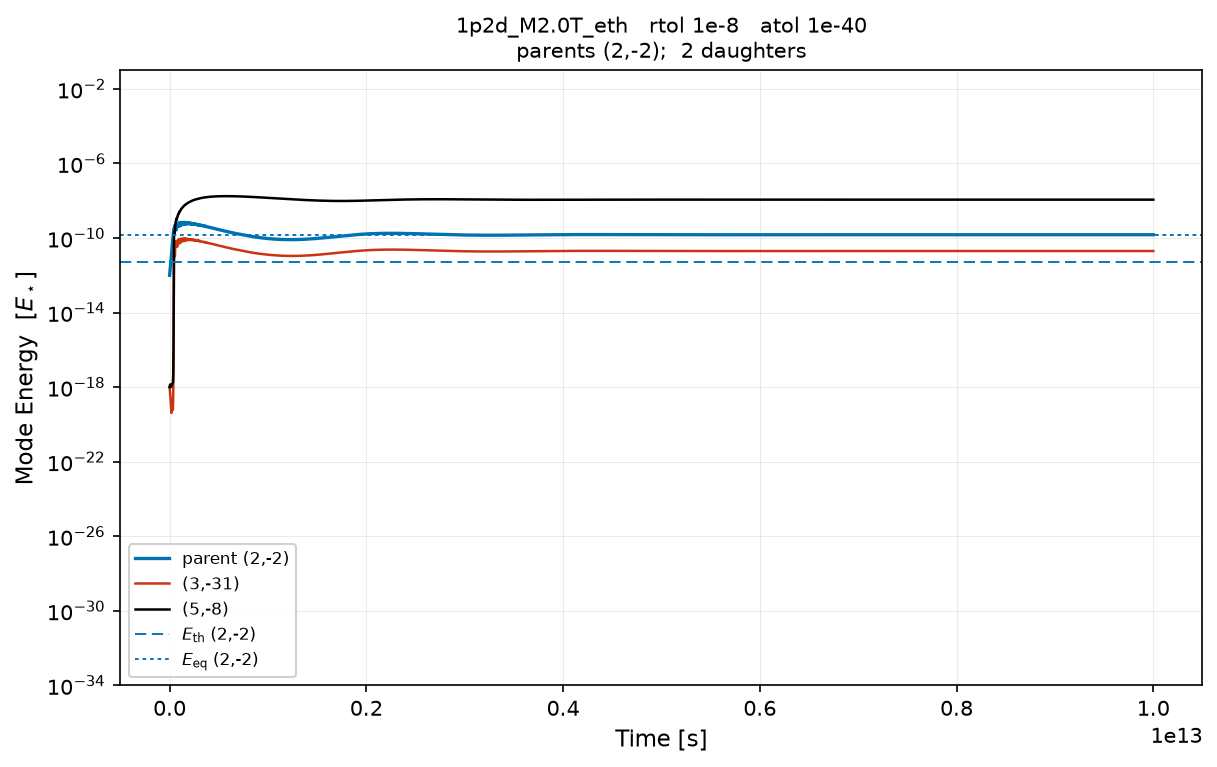
\includegraphics[width=0.21\textwidth,height=0.1323\textwidth]{../plots/rk8pd/1p2d_M2.0T_eth/r1e-8_a1e-40.png} & 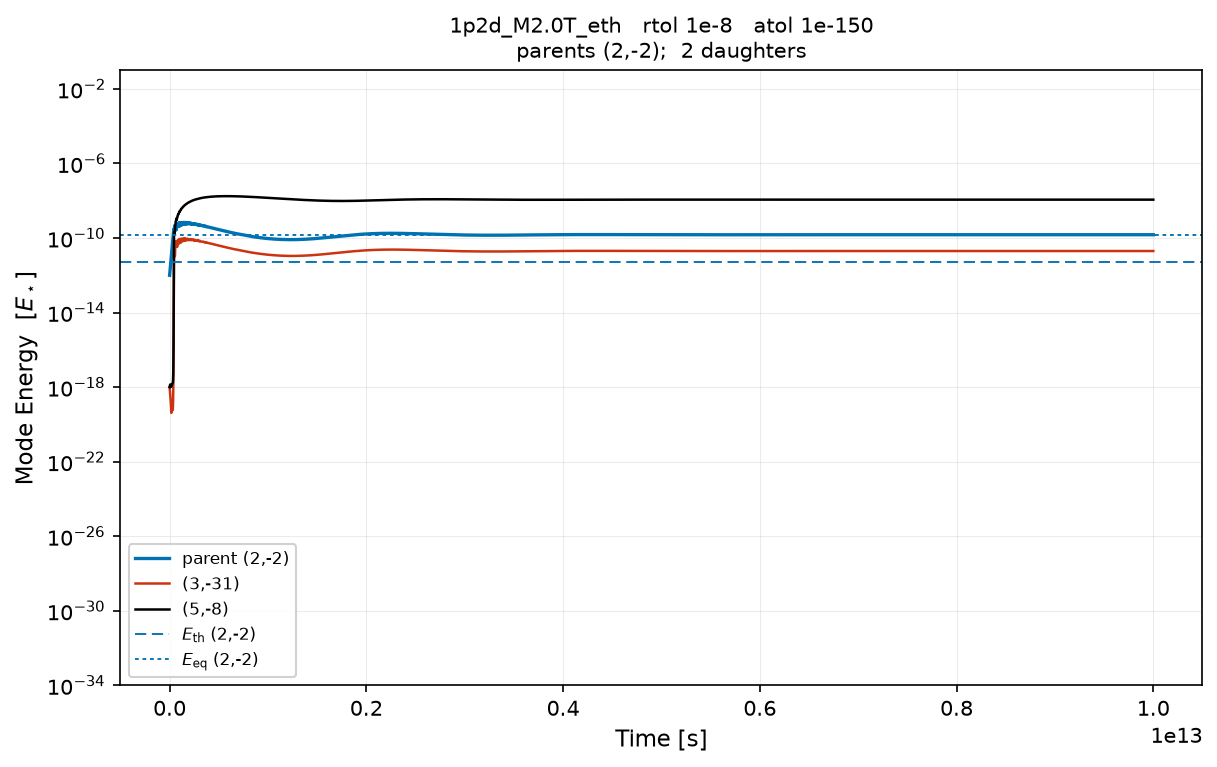
\includegraphics[width=0.21\textwidth,height=0.1323\textwidth]{../plots/rk8pd/1p2d_M2.0T_eth/r1e-8_a1e-150.png} & 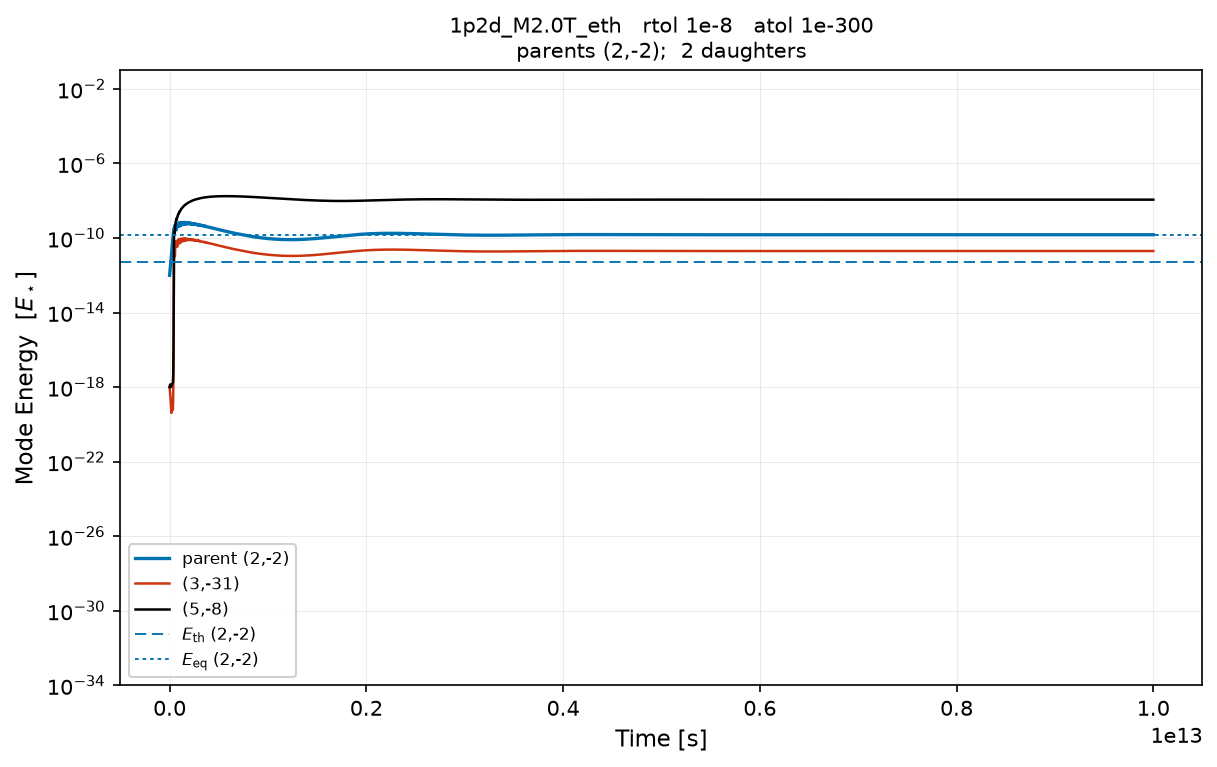
\includegraphics[width=0.21\textwidth,height=0.1323\textwidth]{../plots/rk8pd/1p2d_M2.0T_eth/r1e-8_a1e-300.png} & 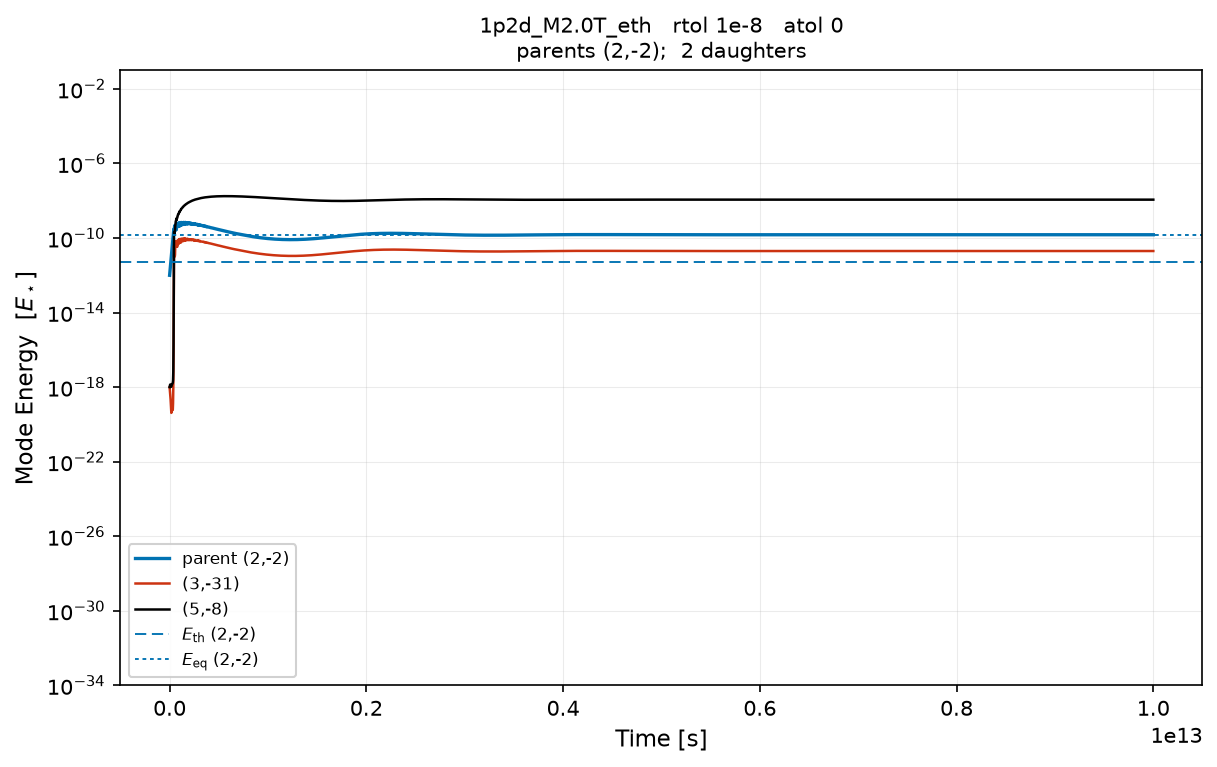
\includegraphics[width=0.21\textwidth,height=0.1323\textwidth]{../plots/rk8pd/1p2d_M2.0T_eth/r1e-8_a0.png} \\[-1pt]
 & \parbox[t]{0.21\textwidth}{\centering\scriptsize 385.4\,k steps, 0.4\,s} & \parbox[t]{0.21\textwidth}{\centering\scriptsize 385.4\,k steps, 0.6\,s} & \parbox[t]{0.21\textwidth}{\centering\scriptsize 385.4\,k steps, 0.8\,s} & \parbox[t]{0.21\textwidth}{\centering\scriptsize 385.4\,k steps, 0.9\,s} \\[2pt]
\rotatebox{90}{\parbox{0.1323\textwidth}{\centering\scriptsize\bfseries BDF, dense analytic Jacobian}} & 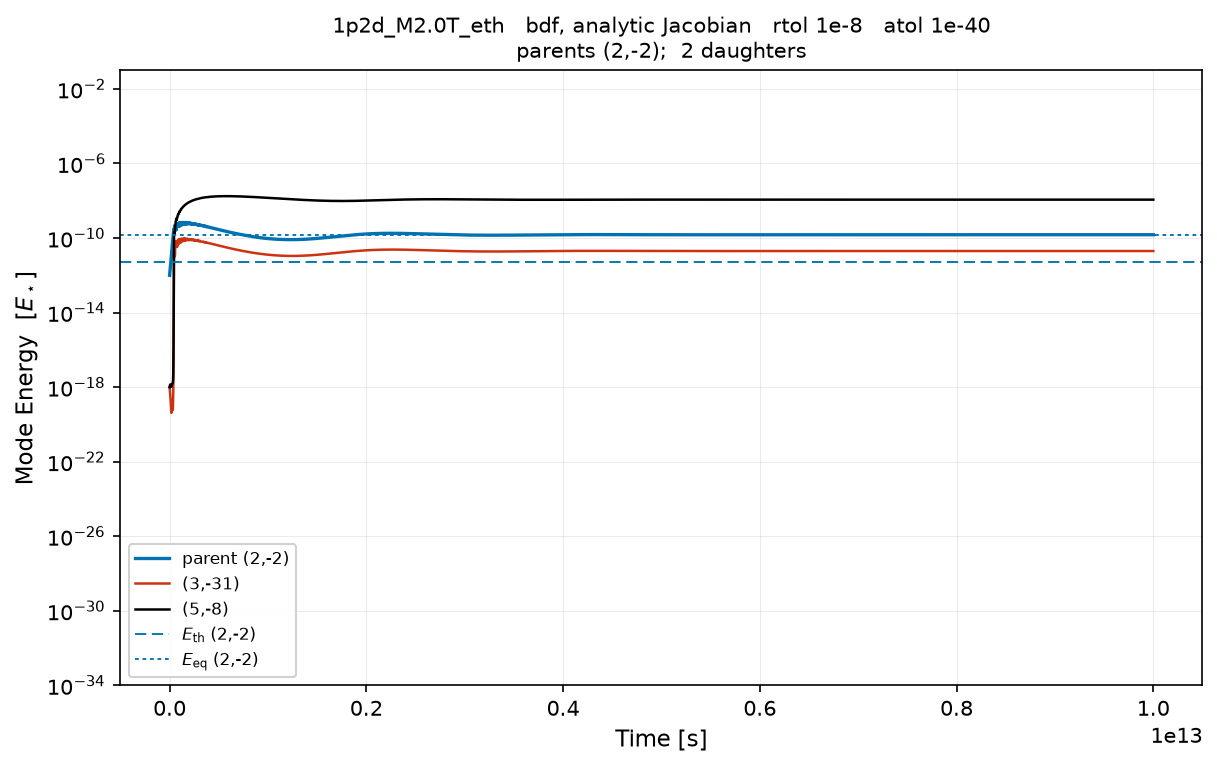
\includegraphics[width=0.21\textwidth,height=0.1323\textwidth]{../plots/bdf/1p2d_M2.0T_eth/r1e-8_a1e-40.png} & 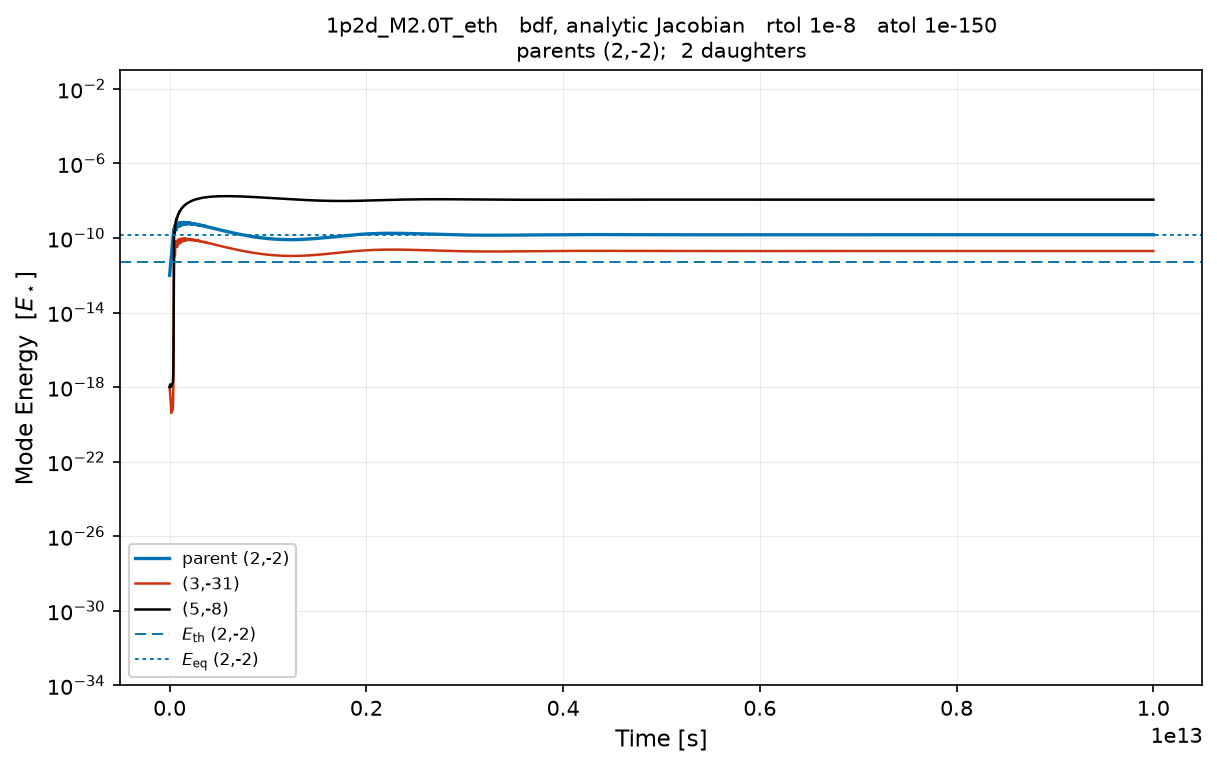
\includegraphics[width=0.21\textwidth,height=0.1323\textwidth]{../plots/bdf/1p2d_M2.0T_eth/r1e-8_a1e-150.png} & 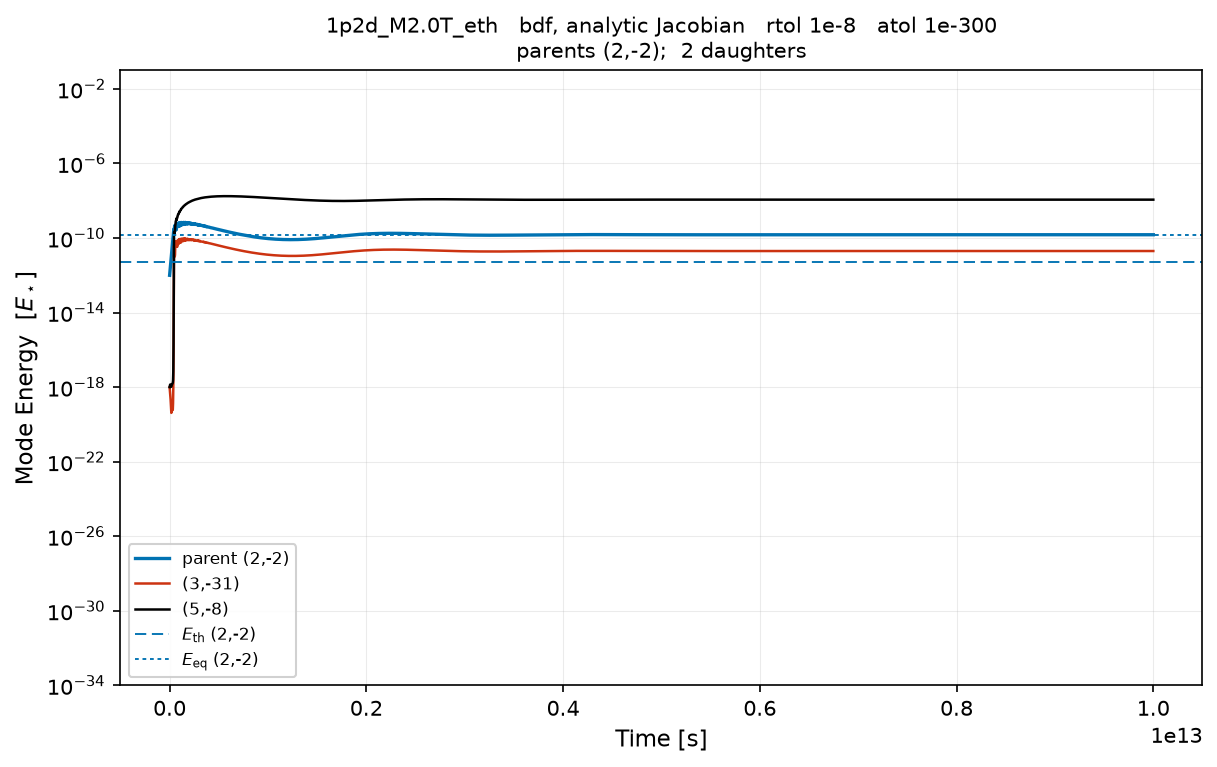
\includegraphics[width=0.21\textwidth,height=0.1323\textwidth]{../plots/bdf/1p2d_M2.0T_eth/r1e-8_a1e-300.png} & 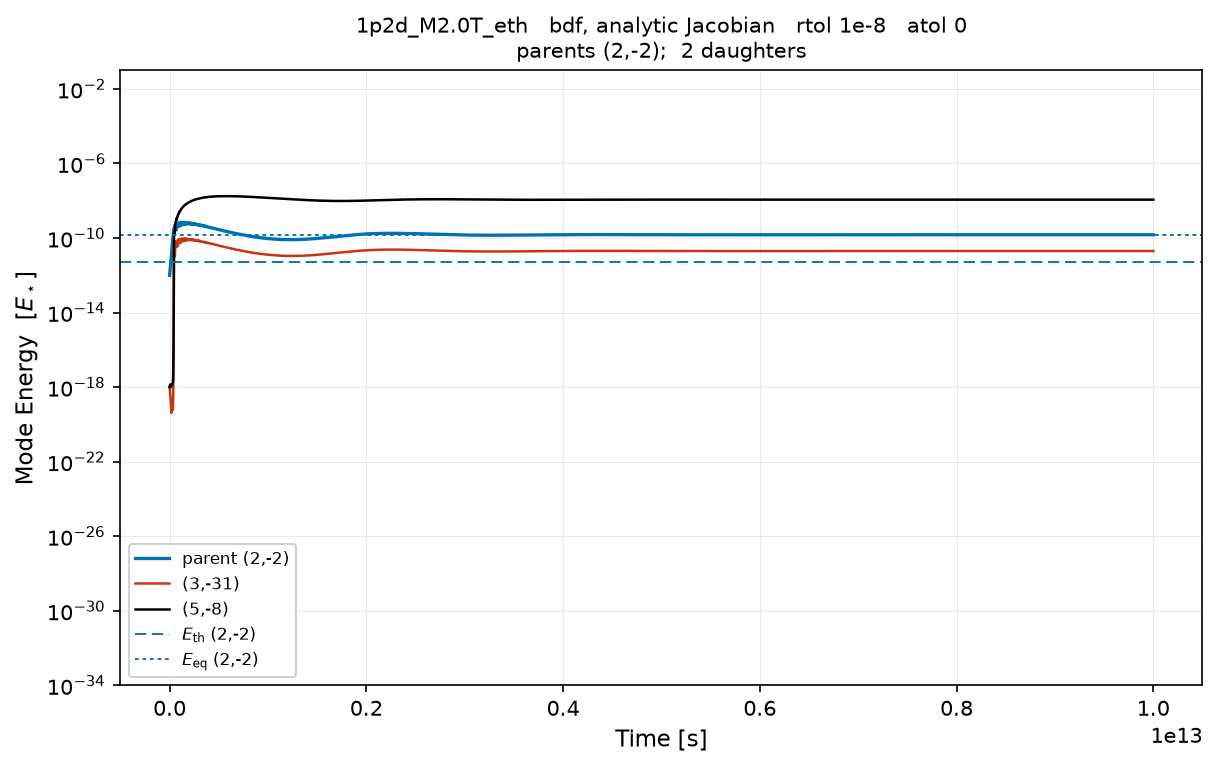
\includegraphics[width=0.21\textwidth,height=0.1323\textwidth]{../plots/bdf/1p2d_M2.0T_eth/r1e-8_a0.png} \\[-1pt]
 & \parbox[t]{0.21\textwidth}{\centering\scriptsize 3.60\,M steps, 3.8\,s} & \parbox[t]{0.21\textwidth}{\centering\scriptsize 3.60\,M steps, 2.5\,s} & \parbox[t]{0.21\textwidth}{\centering\scriptsize 3.60\,M steps, 4.9\,s} & \parbox[t]{0.21\textwidth}{\centering\scriptsize 3.60\,M steps, 2.8\,s} \\[2pt]
\rotatebox{90}{\parbox{0.1323\textwidth}{\centering\scriptsize\bfseries BDF-Krylov, band full}} & 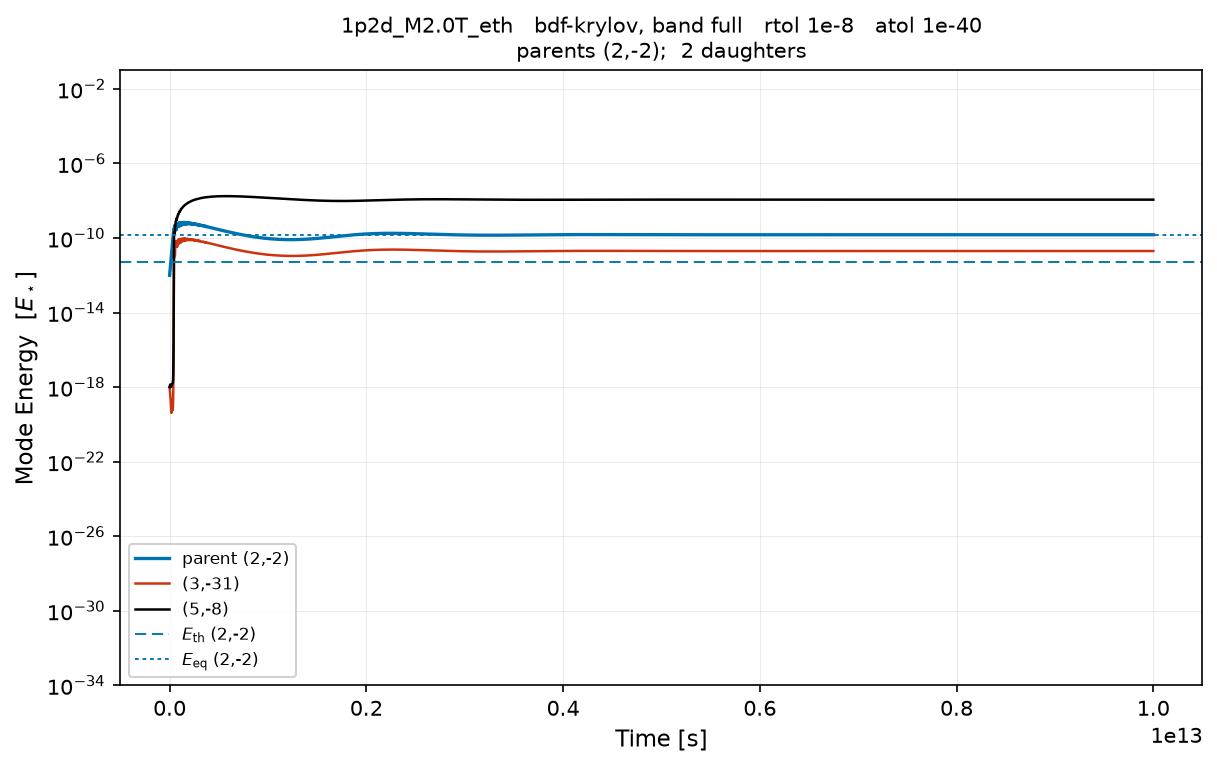
\includegraphics[width=0.21\textwidth,height=0.1323\textwidth]{../plots/krylov_full/1p2d_M2.0T_eth/r1e-8_a1e-40.png} & 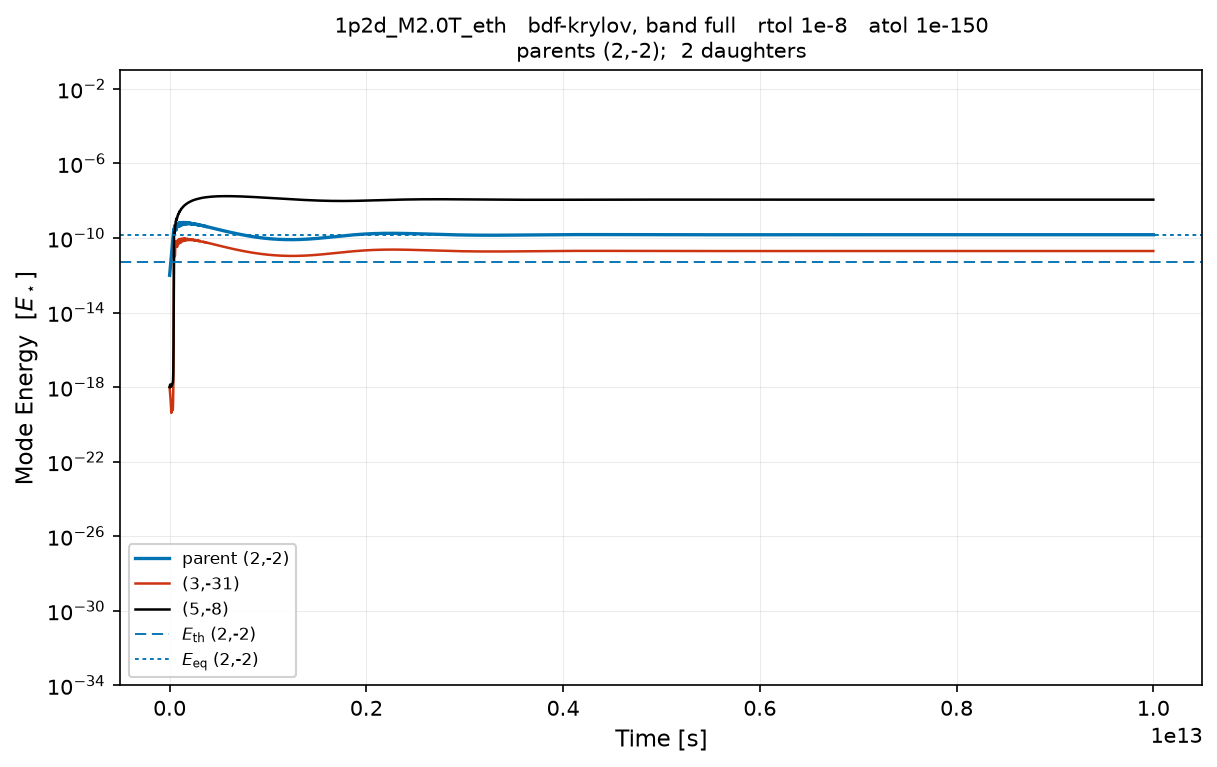
\includegraphics[width=0.21\textwidth,height=0.1323\textwidth]{../plots/krylov_full/1p2d_M2.0T_eth/r1e-8_a1e-150.png} & 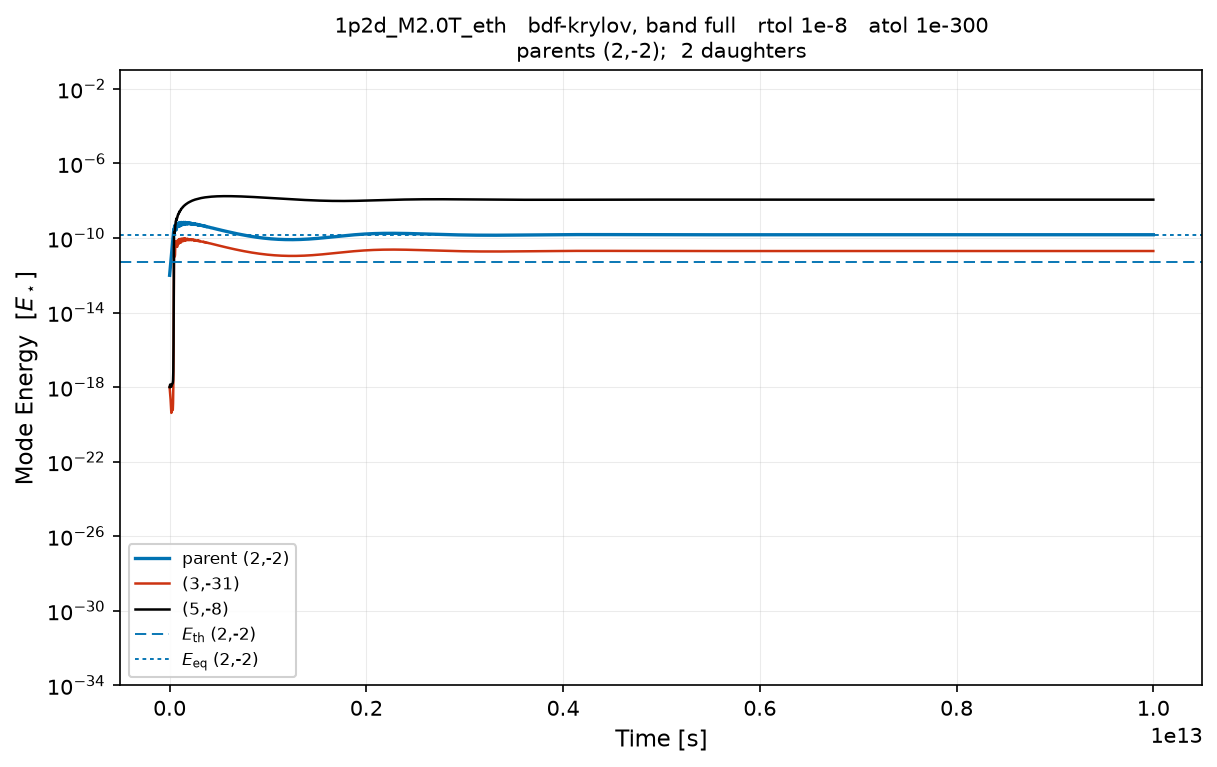
\includegraphics[width=0.21\textwidth,height=0.1323\textwidth]{../plots/krylov_full/1p2d_M2.0T_eth/r1e-8_a1e-300.png} & 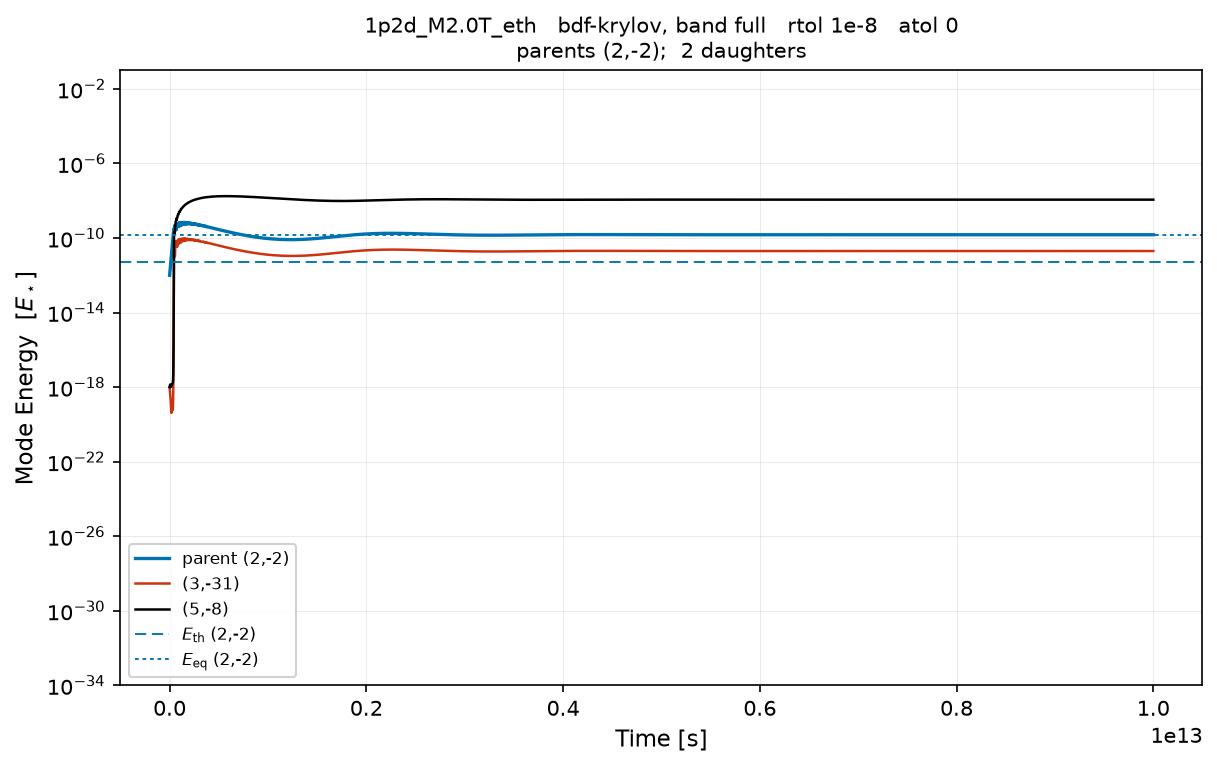
\includegraphics[width=0.21\textwidth,height=0.1323\textwidth]{../plots/krylov_full/1p2d_M2.0T_eth/r1e-8_a0.png} \\[-1pt]
 & \parbox[t]{0.21\textwidth}{\centering\scriptsize 3.55\,M steps, 6.6\,s} & \parbox[t]{0.21\textwidth}{\centering\scriptsize 3.55\,M steps, 4.2\,s} & \parbox[t]{0.21\textwidth}{\centering\scriptsize 3.55\,M steps, 6.6\,s} & \parbox[t]{0.21\textwidth}{\centering\scriptsize 3.55\,M steps, 6.9\,s} \\[2pt]
\rotatebox{90}{\parbox{0.1323\textwidth}{\centering\scriptsize\bfseries BDF-Krylov, band 3}} & 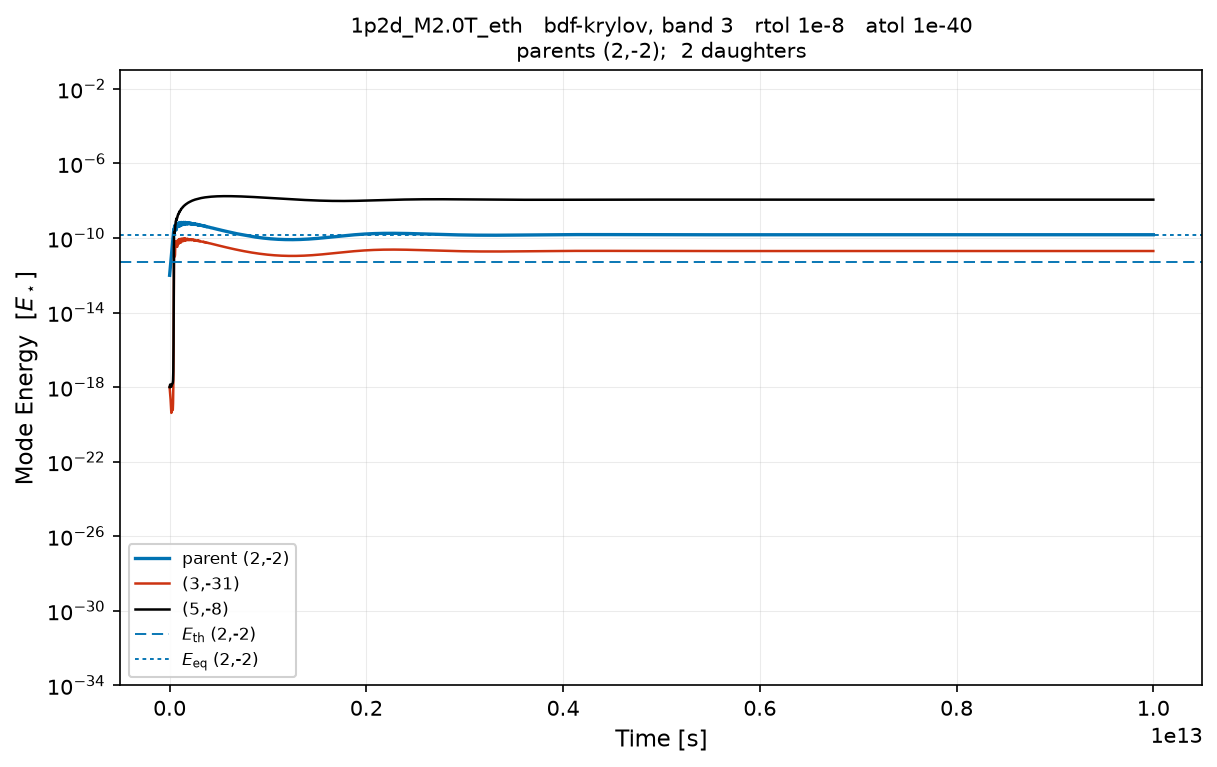
\includegraphics[width=0.21\textwidth,height=0.1323\textwidth]{../plots/krylov_b3/1p2d_M2.0T_eth/r1e-8_a1e-40.png} & 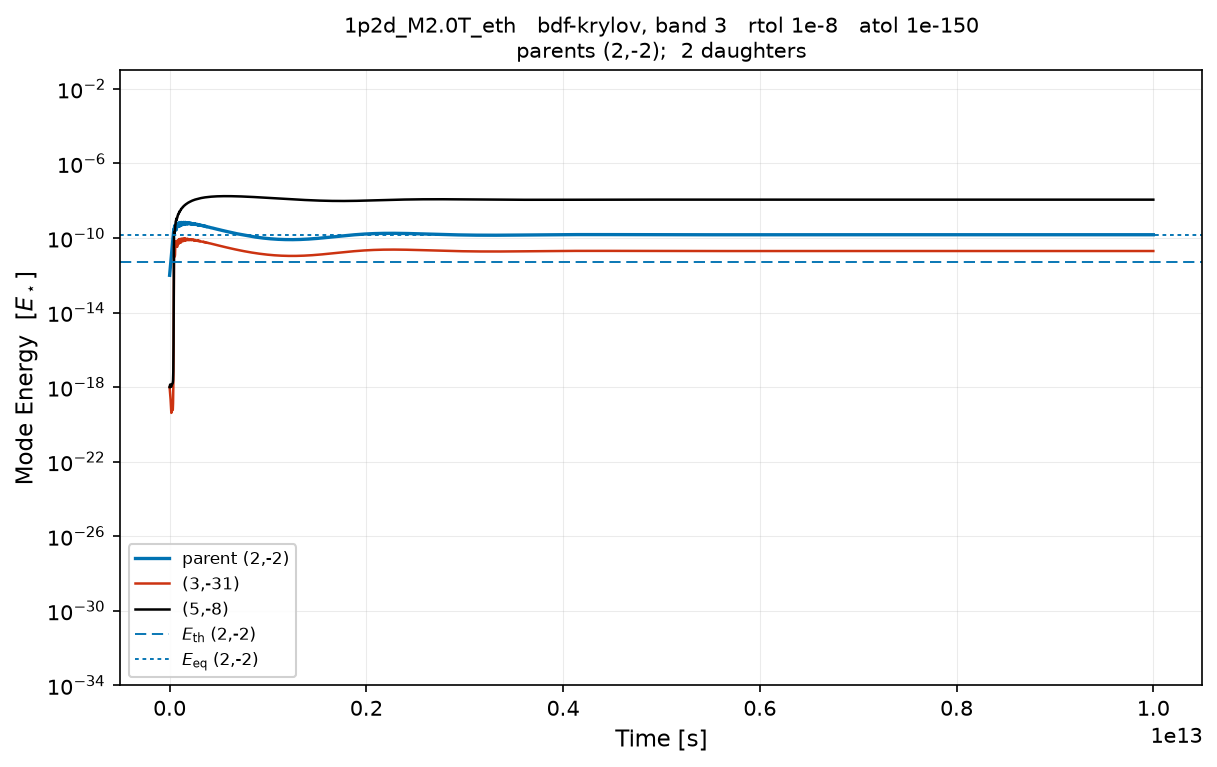
\includegraphics[width=0.21\textwidth,height=0.1323\textwidth]{../plots/krylov_b3/1p2d_M2.0T_eth/r1e-8_a1e-150.png} & 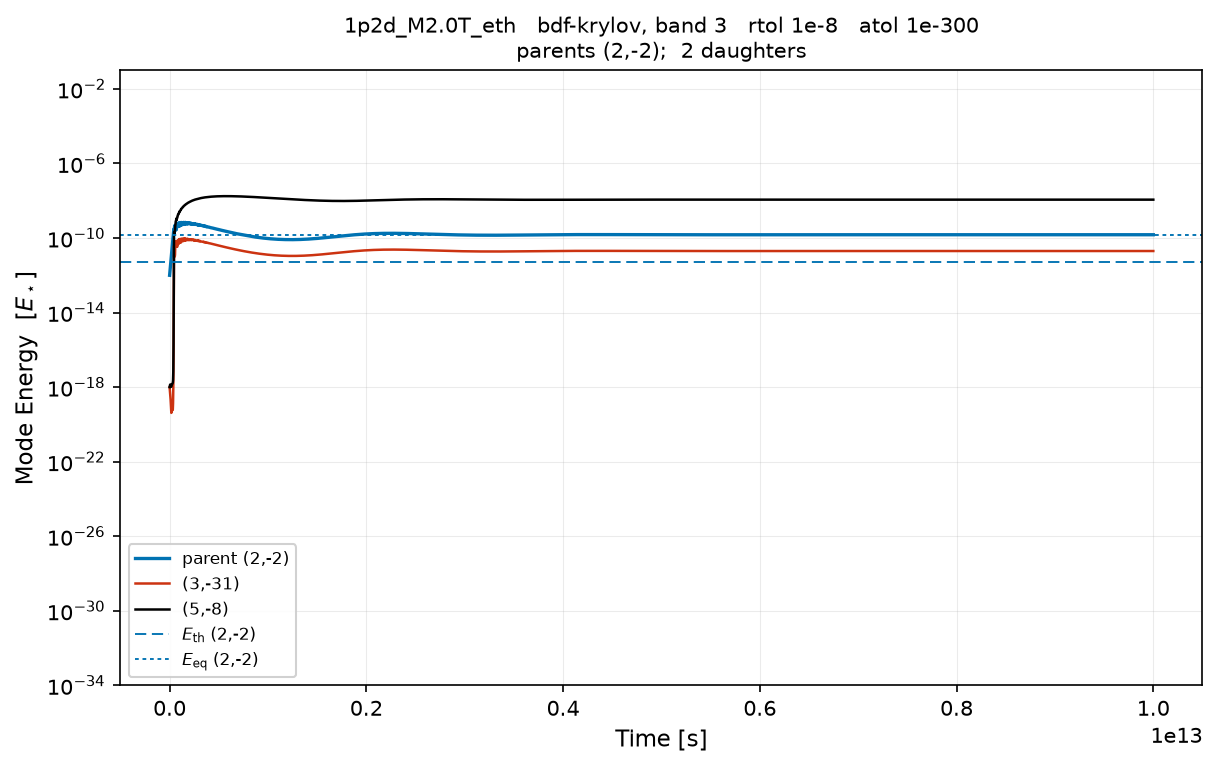
\includegraphics[width=0.21\textwidth,height=0.1323\textwidth]{../plots/krylov_b3/1p2d_M2.0T_eth/r1e-8_a1e-300.png} & 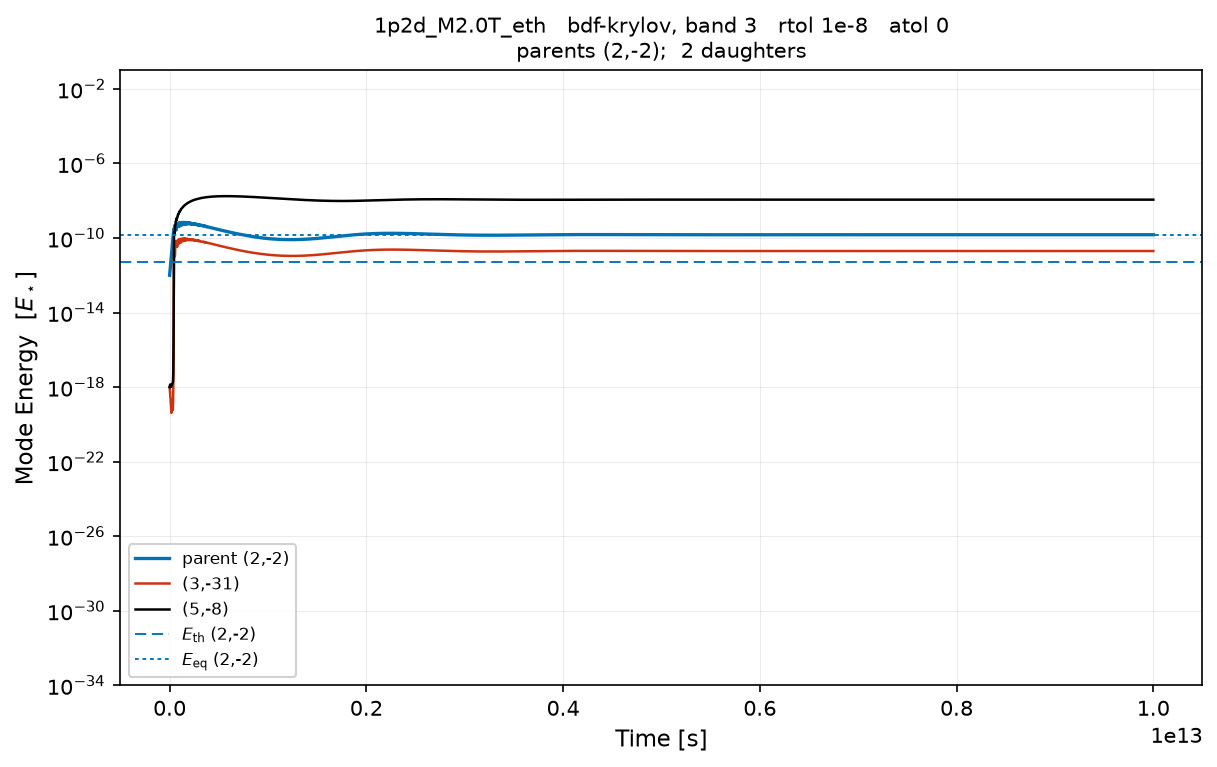
\includegraphics[width=0.21\textwidth,height=0.1323\textwidth]{../plots/krylov_b3/1p2d_M2.0T_eth/r1e-8_a0.png} \\[-1pt]
 & \parbox[t]{0.21\textwidth}{\centering\scriptsize 3.54\,M steps, 4.4\,s} & \parbox[t]{0.21\textwidth}{\centering\scriptsize 3.54\,M steps, 6.8\,s} & \parbox[t]{0.21\textwidth}{\centering\scriptsize 3.54\,M steps, 6.5\,s} & \parbox[t]{0.21\textwidth}{\centering\scriptsize 3.54\,M steps, 6.8\,s} \\[2pt]
\rotatebox{90}{\parbox{0.1323\textwidth}{\centering\scriptsize\bfseries Adams, fixed point}} & 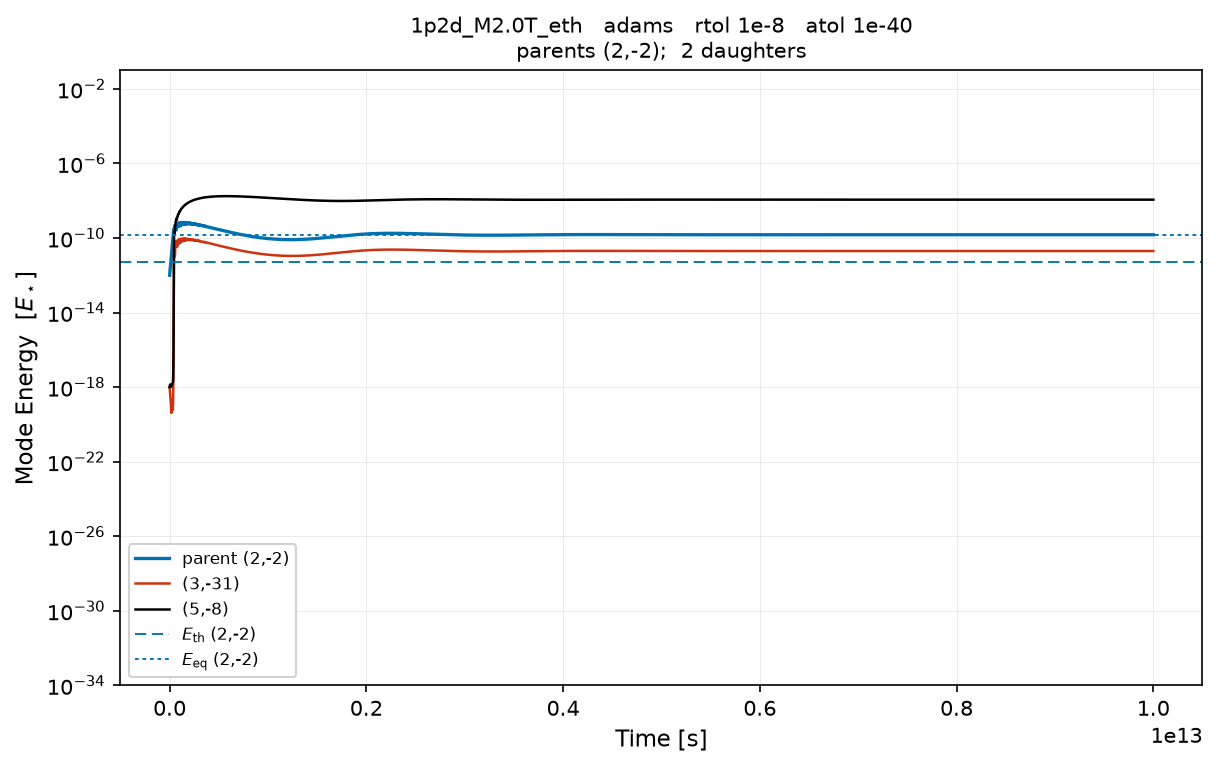
\includegraphics[width=0.21\textwidth,height=0.1323\textwidth]{../plots/adams/1p2d_M2.0T_eth/r1e-8_a1e-40.png} & 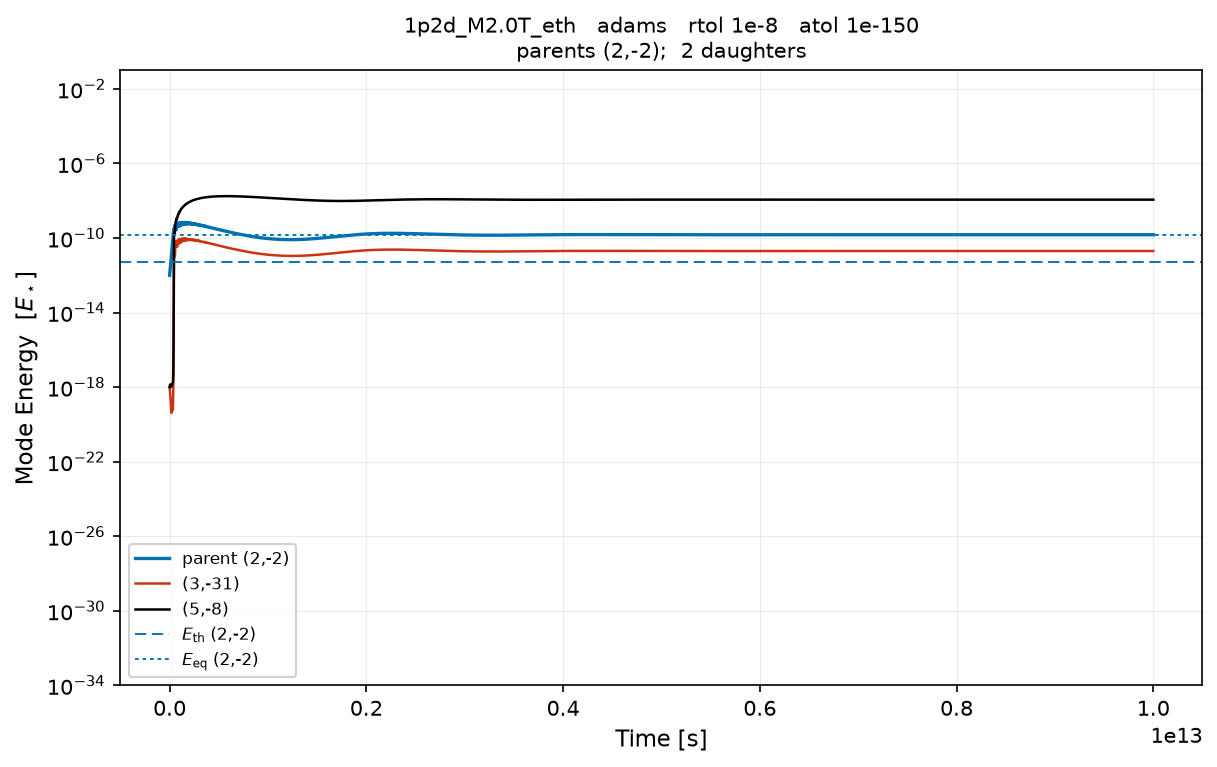
\includegraphics[width=0.21\textwidth,height=0.1323\textwidth]{../plots/adams/1p2d_M2.0T_eth/r1e-8_a1e-150.png} & 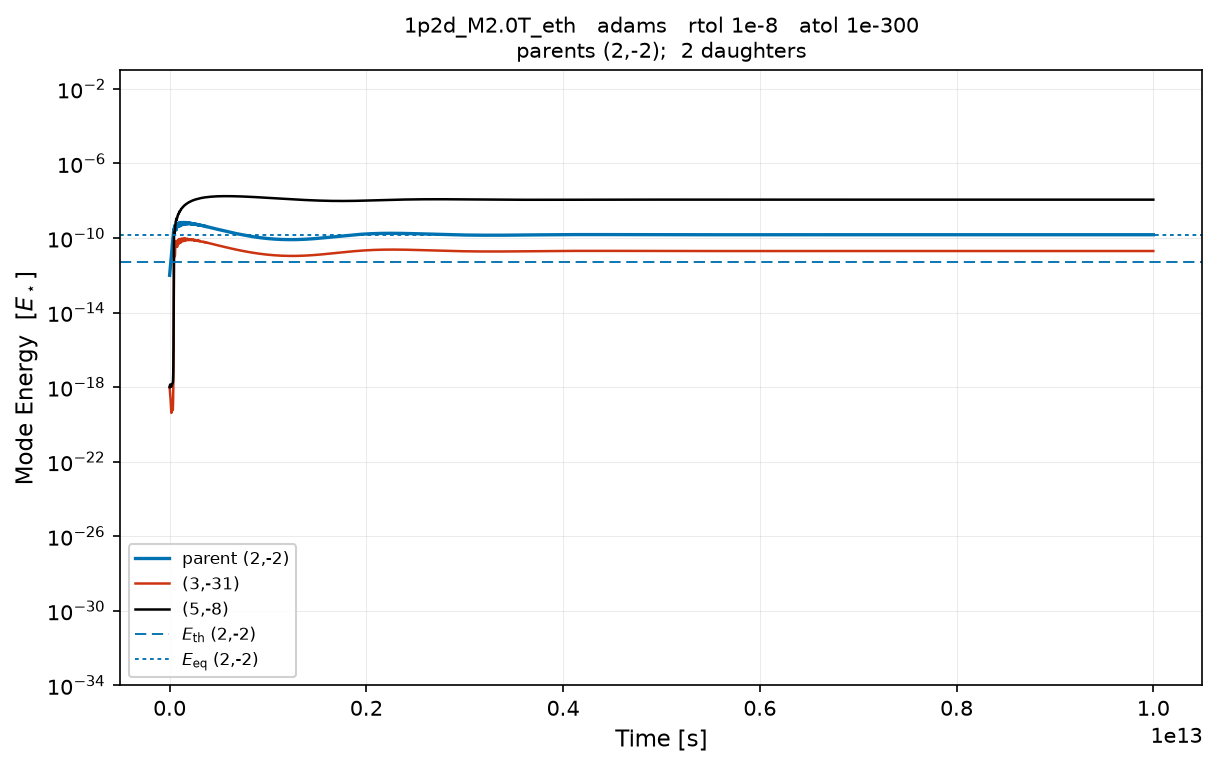
\includegraphics[width=0.21\textwidth,height=0.1323\textwidth]{../plots/adams/1p2d_M2.0T_eth/r1e-8_a1e-300.png} & 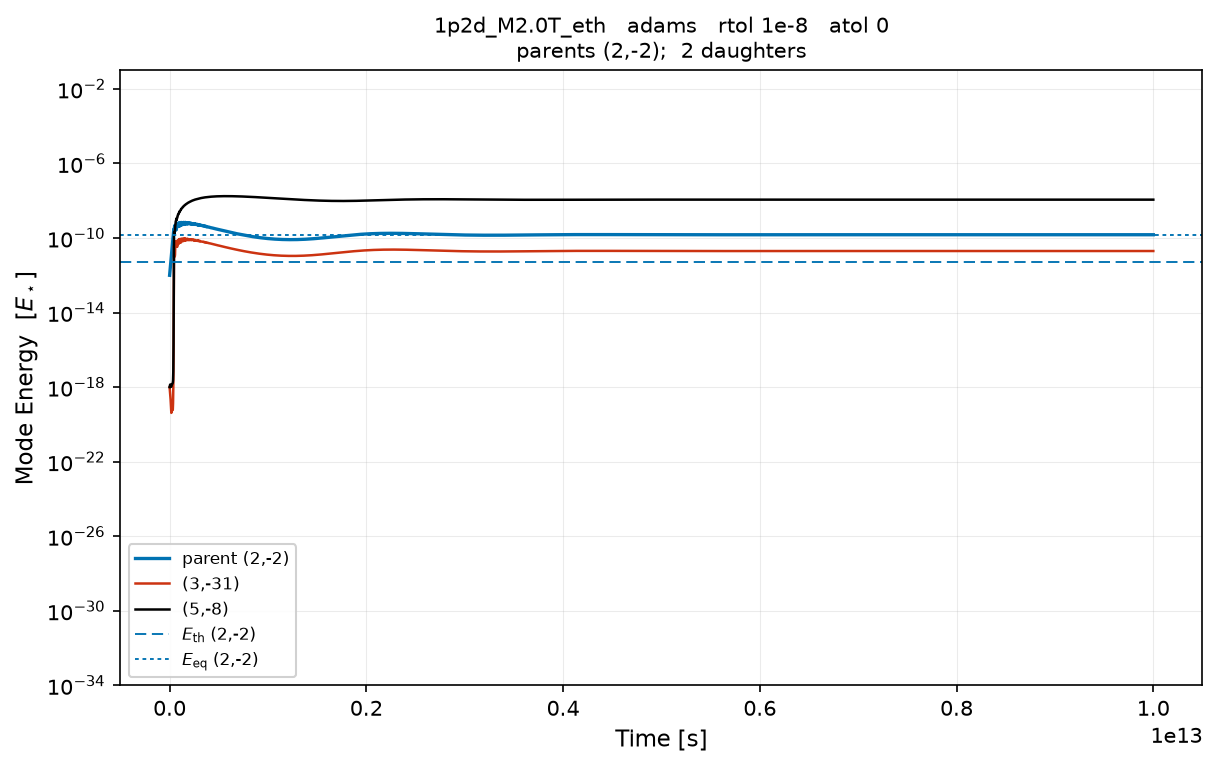
\includegraphics[width=0.21\textwidth,height=0.1323\textwidth]{../plots/adams/1p2d_M2.0T_eth/r1e-8_a0.png} \\[-1pt]
 & \parbox[t]{0.21\textwidth}{\centering\scriptsize 2.04\,M steps, 2.6\,s} & \parbox[t]{0.21\textwidth}{\centering\scriptsize 2.04\,M steps, 2.6\,s} & \parbox[t]{0.21\textwidth}{\centering\scriptsize 2.04\,M steps, 2.6\,s} & \parbox[t]{0.21\textwidth}{\centering\scriptsize 2.04\,M steps, 2.6\,s} \\[2pt]
\end{tabular}\par}
\par\noindent{\scriptsize\setlength\tabcolsep{3.5pt}\renewcommand\arraystretch{0.92}
\begin{tabular}{@{}llllrrrrrrr@{}}
\toprule
integrator & atol & stop & $t_{\rm stop}$ [s] & steps & rejected & RHS & Jac. & NL it. & lin. it. & wall [s] \\
\midrule
rk8pd & $10^{-40}$ & end & $1.00\times10^{13}$ & 385.4\,k & 83.7\,k & 5.01\,M & -- & -- & -- & 0.4 \\
 & $10^{-150}$ & end & $1.00\times10^{13}$ & 385.4\,k & 83.7\,k & 5.01\,M & -- & -- & -- & 0.6 \\
 & $10^{-300}$ & end & $1.00\times10^{13}$ & 385.4\,k & 83.7\,k & 5.01\,M & -- & -- & -- & 0.8 \\
 & $0$ & end & $1.00\times10^{13}$ & 385.4\,k & 83.7\,k & 5.01\,M & -- & -- & -- & 0.9 \\
\addlinespace[2pt]
BDF, dense analytic Jacobian & $10^{-40}$ & end & $1.00\times10^{13}$ & 3.60\,M & 59.0\,k & 3.99\,M & 77.3\,k & 3.99\,M & -- & 3.8 \\
 & $10^{-150}$ & end & $1.00\times10^{13}$ & 3.60\,M & 59.0\,k & 3.99\,M & 77.3\,k & 3.99\,M & -- & 2.5 \\
 & $10^{-300}$ & end & $1.00\times10^{13}$ & 3.60\,M & 59.0\,k & 3.99\,M & 77.3\,k & 3.99\,M & -- & 4.9 \\
 & $0$ & end & $1.00\times10^{13}$ & 3.60\,M & 59.0\,k & 3.99\,M & 77.3\,k & 3.99\,M & -- & 2.8 \\
\addlinespace[2pt]
BDF-Krylov, band full & $10^{-40}$ & end & $1.00\times10^{13}$ & 3.55\,M & 60.9\,k & 7.98\,M & 73.4\,k & 3.91\,M & 3.62\,M & 6.6 \\
 & $10^{-150}$ & end & $1.00\times10^{13}$ & 3.55\,M & 60.9\,k & 7.98\,M & 73.4\,k & 3.91\,M & 3.62\,M & 4.2 \\
 & $10^{-300}$ & end & $1.00\times10^{13}$ & 3.55\,M & 60.9\,k & 7.98\,M & 73.4\,k & 3.91\,M & 3.62\,M & 6.6 \\
 & $0$ & end & $1.00\times10^{13}$ & 3.55\,M & 60.9\,k & 7.98\,M & 73.4\,k & 3.91\,M & 3.62\,M & 6.9 \\
\addlinespace[2pt]
BDF-Krylov, band 3 & $10^{-40}$ & end & $1.00\times10^{13}$ & 3.54\,M & 61.1\,k & 7.98\,M & 73.2\,k & 3.91\,M & 3.63\,M & 4.4 \\
 & $10^{-150}$ & end & $1.00\times10^{13}$ & 3.54\,M & 61.1\,k & 7.98\,M & 73.2\,k & 3.91\,M & 3.63\,M & 6.8 \\
 & $10^{-300}$ & end & $1.00\times10^{13}$ & 3.54\,M & 61.1\,k & 7.98\,M & 73.2\,k & 3.91\,M & 3.63\,M & 6.5 \\
 & $0$ & end & $1.00\times10^{13}$ & 3.54\,M & 61.1\,k & 7.98\,M & 73.2\,k & 3.91\,M & 3.63\,M & 6.8 \\
\addlinespace[2pt]
Adams, fixed point & $10^{-40}$ & end & $1.00\times10^{13}$ & 2.04\,M & 134.1\,k & 3.35\,M & -- & 3.34\,M & -- & 2.6 \\
 & $10^{-150}$ & end & $1.00\times10^{13}$ & 2.04\,M & 134.1\,k & 3.35\,M & -- & 3.34\,M & -- & 2.6 \\
 & $10^{-300}$ & end & $1.00\times10^{13}$ & 2.04\,M & 134.1\,k & 3.35\,M & -- & 3.34\,M & -- & 2.6 \\
 & $0$ & end & $1.00\times10^{13}$ & 2.04\,M & 134.1\,k & 3.35\,M & -- & 3.34\,M & -- & 2.6 \\
\bottomrule
\end{tabular}}

\clearpage
\subsection{\texttt{1p2d\_M2.0\_dgamma}}\label{net:1p2d_M2.0_dgamma}
\noindent\begin{minipage}[t]{0.43\textwidth}\vspace{0pt}\footnotesize
\begin{tabular}{@{}rrlrr@{}}
\toprule
id & gen & $(\ell,n)$ & $\omega$ [rad\,s$^{-1}$] & $\gamma$ [s$^{-1}$] \\
\midrule
0 & 0 & (1,$-$1) & $7.581\times10^{-4}$ & $-2.276\times10^{-10}$ \\
1 & 1 & (5,$-$9) & $6.198\times10^{-4}$ & $4.584\times10^{-13}$ \\
2 & 1 & (6,$-$56) & $1.377\times10^{-4}$ & $2.817\times10^{-9}$ \\
\bottomrule
\end{tabular}
\end{minipage}\hfill
\begin{minipage}[t]{0.55\textwidth}\vspace{0pt}\footnotesize
\textbf{Model} \texttt{dsct\_M2.0}, rule dgamma, $N=1$, cut 0.15,
closure 0.005; 3 modes, 1 triplet(s).\\[2pt]
\textbf{Selecting pairs}\\ (1,$-$1) $\to$ (5,$-$9) + (6,$-$56): $\Delta/\omega_a=-6.83\times10^{-4}$, $\kappa=+0.085$, $E_{\rm th}=1.75\times10^{-8}$, $E_{\rm eq}=2.07\times10^{-8}$\\[2pt]
Deep dips between bursts.
\end{minipage}

\par\smallskip{\centering\begin{tabular}{@{}c@{\hspace{2pt}}c@{\hspace{2pt}}c@{\hspace{2pt}}c@{\hspace{2pt}}c@{}}
 & \small atol $10^{-40}$ & \small atol $10^{-150}$ & \small atol $10^{-300}$ & \small atol $0$ \\[1pt]
\rotatebox{90}{\parbox{0.1323\textwidth}{\centering\scriptsize\bfseries rk8pd}} & 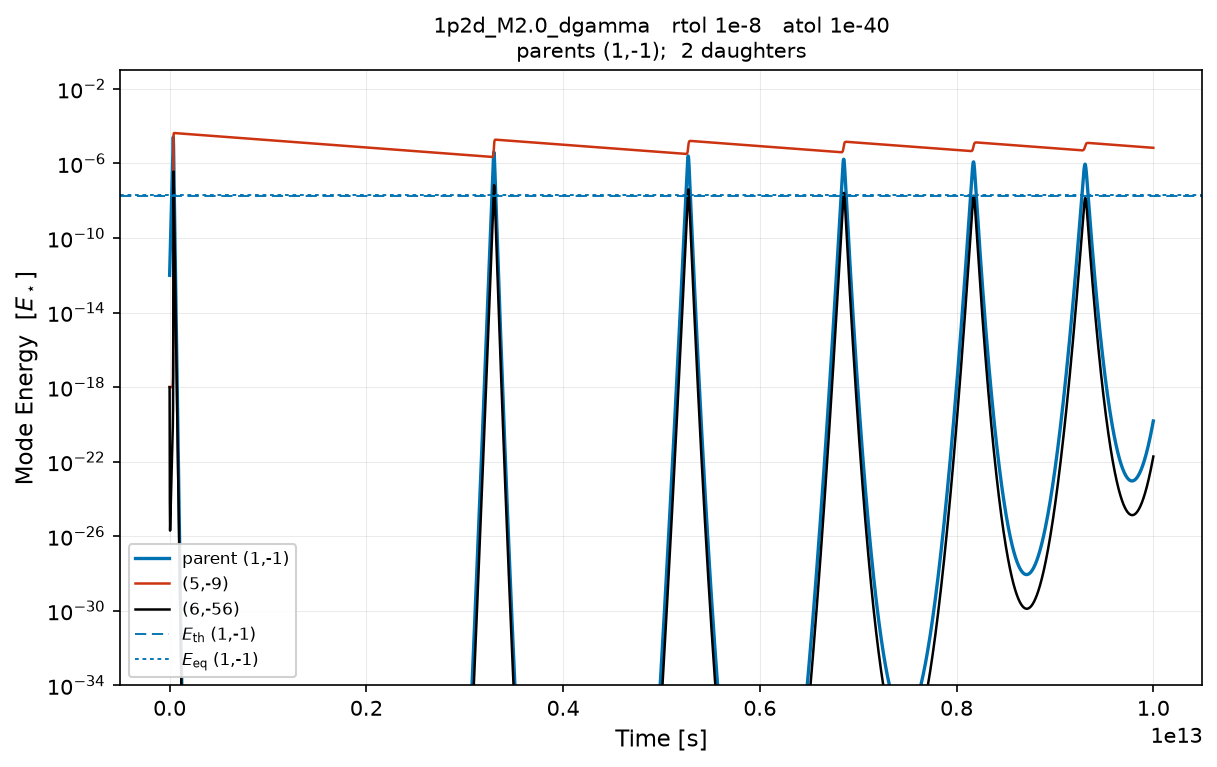
\includegraphics[width=0.21\textwidth,height=0.1323\textwidth]{../plots/rk8pd/1p2d_M2.0_dgamma/r1e-8_a1e-40.png} & 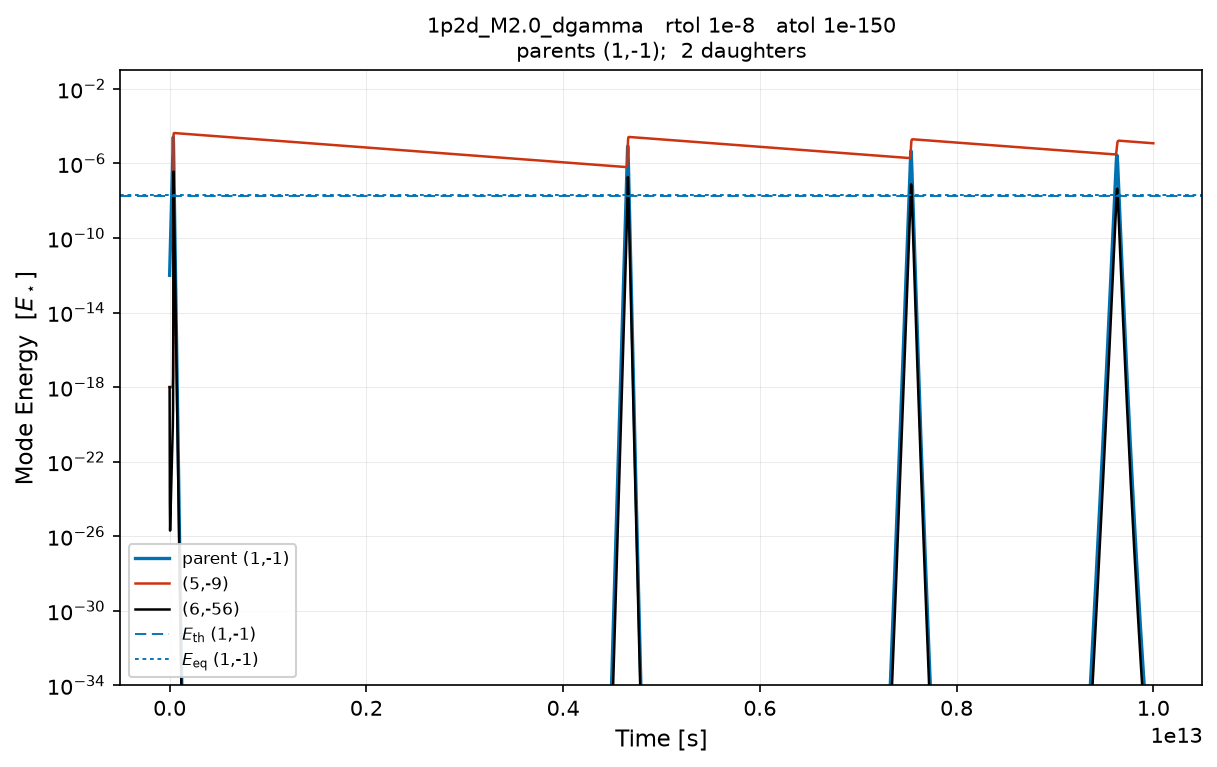
\includegraphics[width=0.21\textwidth,height=0.1323\textwidth]{../plots/rk8pd/1p2d_M2.0_dgamma/r1e-8_a1e-150.png} & 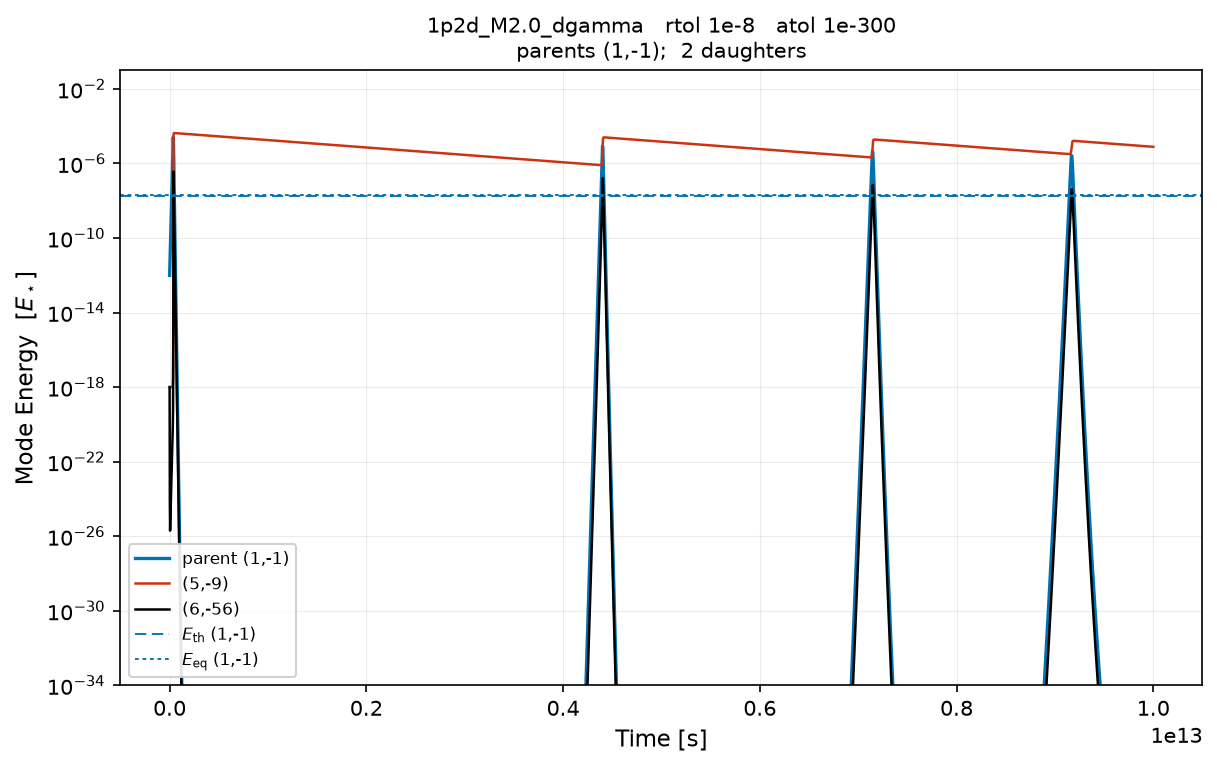
\includegraphics[width=0.21\textwidth,height=0.1323\textwidth]{../plots/rk8pd/1p2d_M2.0_dgamma/r1e-8_a1e-300.png} & 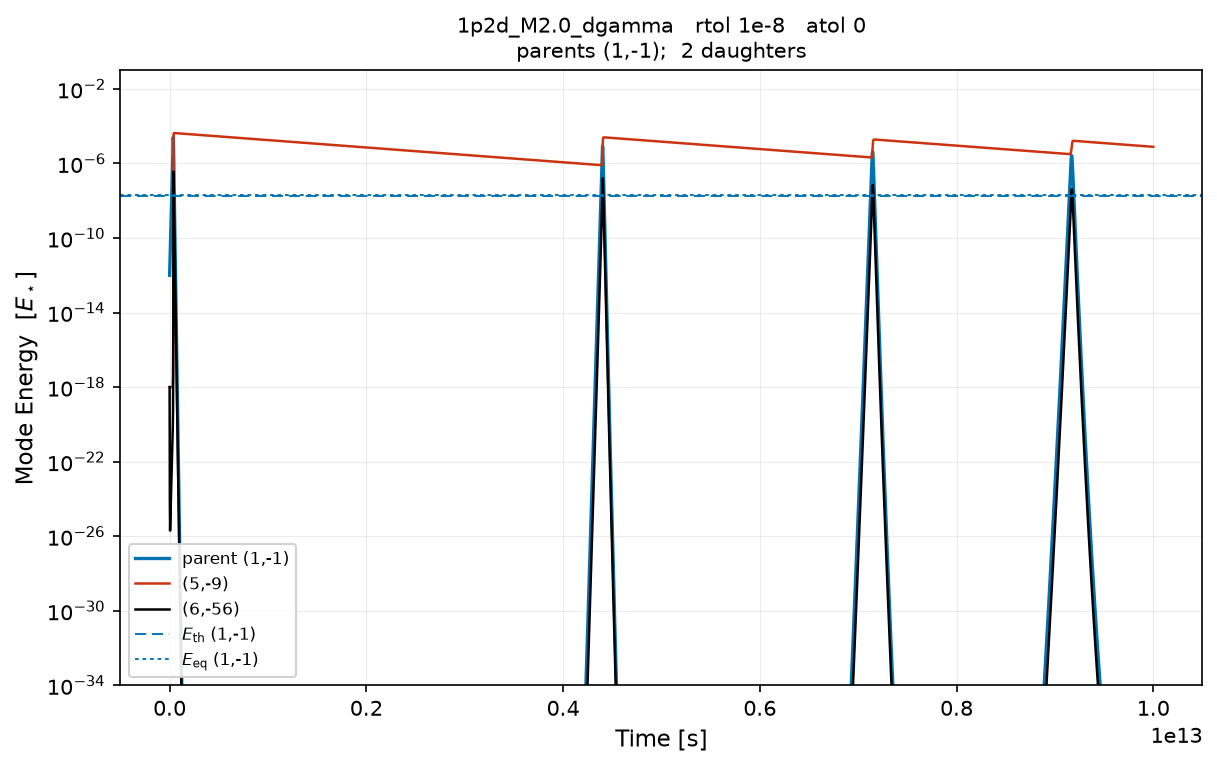
\includegraphics[width=0.21\textwidth,height=0.1323\textwidth]{../plots/rk8pd/1p2d_M2.0_dgamma/r1e-8_a0.png} \\[-1pt]
 & \parbox[t]{0.21\textwidth}{\centering\scriptsize 6.61\,M steps, 9.5\,s} & \parbox[t]{0.21\textwidth}{\centering\scriptsize 8.24\,M steps, 15.6\,s} & \parbox[t]{0.21\textwidth}{\centering\scriptsize 9.26\,M steps, 13.5\,s} & \parbox[t]{0.21\textwidth}{\centering\scriptsize 9.26\,M steps, 20.4\,s} \\[2pt]
\rotatebox{90}{\parbox{0.1323\textwidth}{\centering\scriptsize\bfseries BDF, dense analytic Jacobian}} & 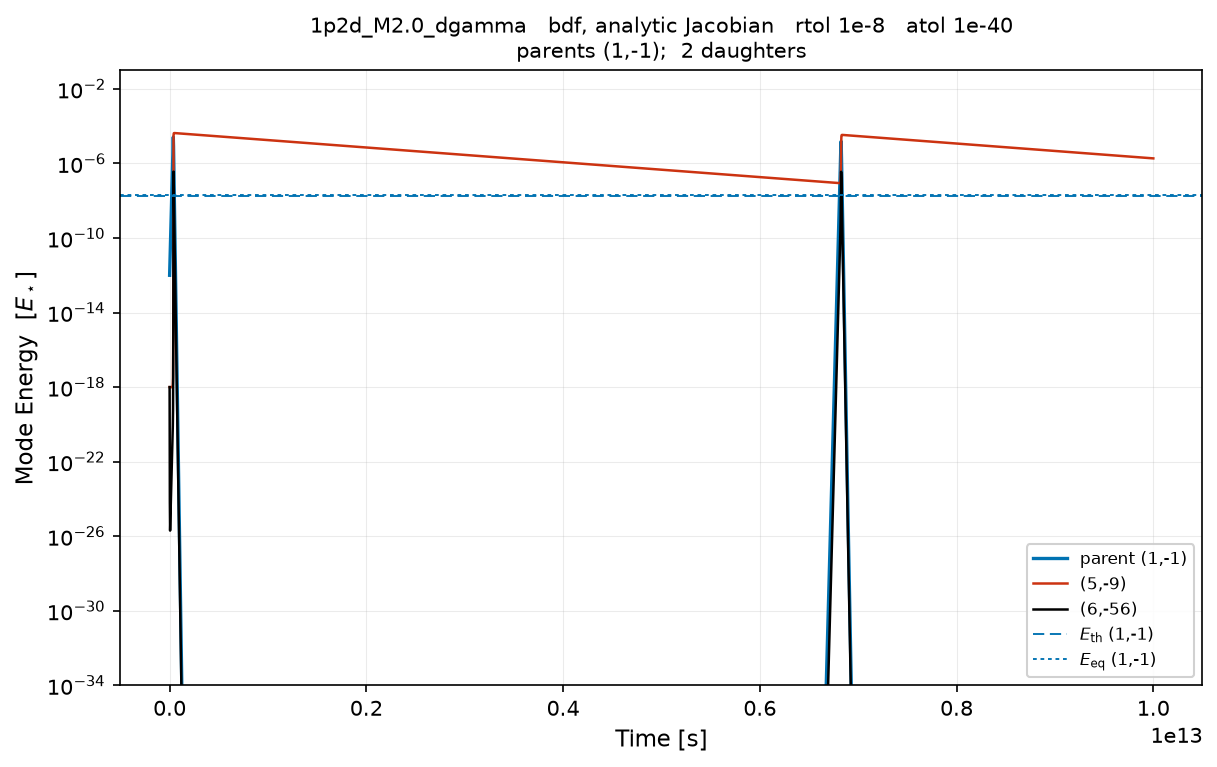
\includegraphics[width=0.21\textwidth,height=0.1323\textwidth]{../plots/bdf/1p2d_M2.0_dgamma/r1e-8_a1e-40.png} & 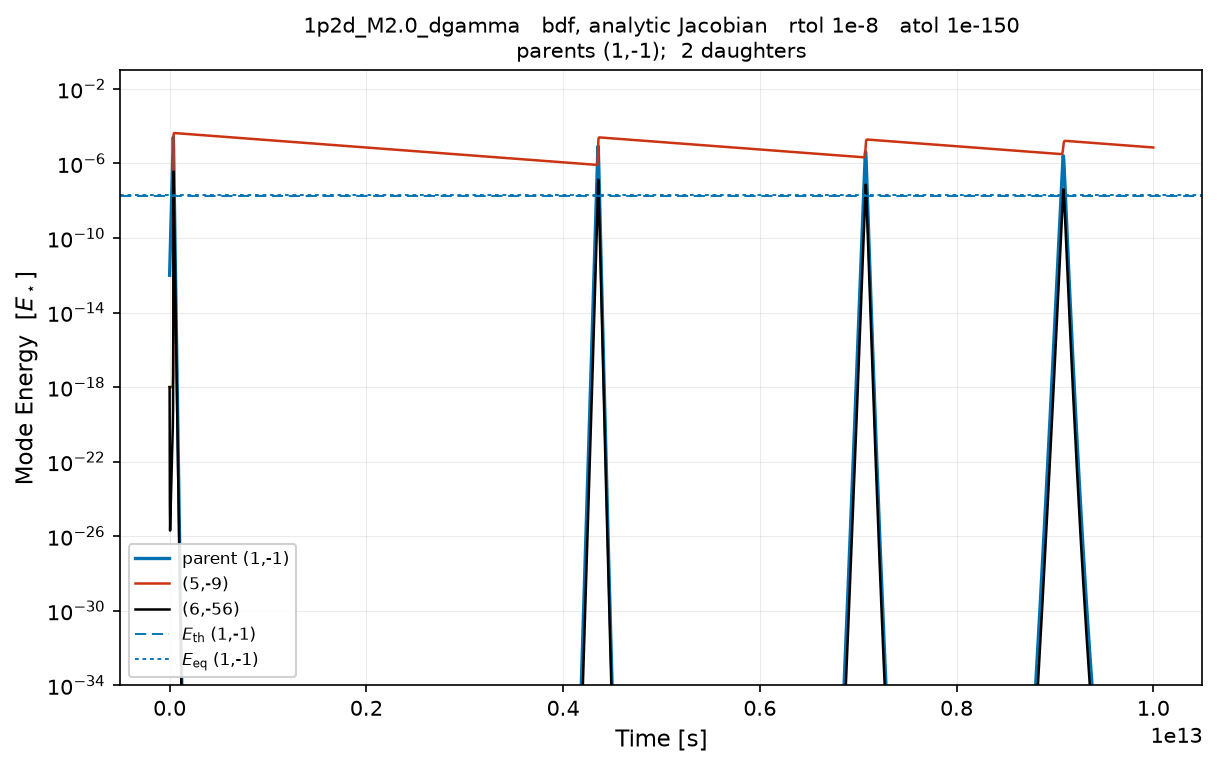
\includegraphics[width=0.21\textwidth,height=0.1323\textwidth]{../plots/bdf/1p2d_M2.0_dgamma/r1e-8_a1e-150.png} & 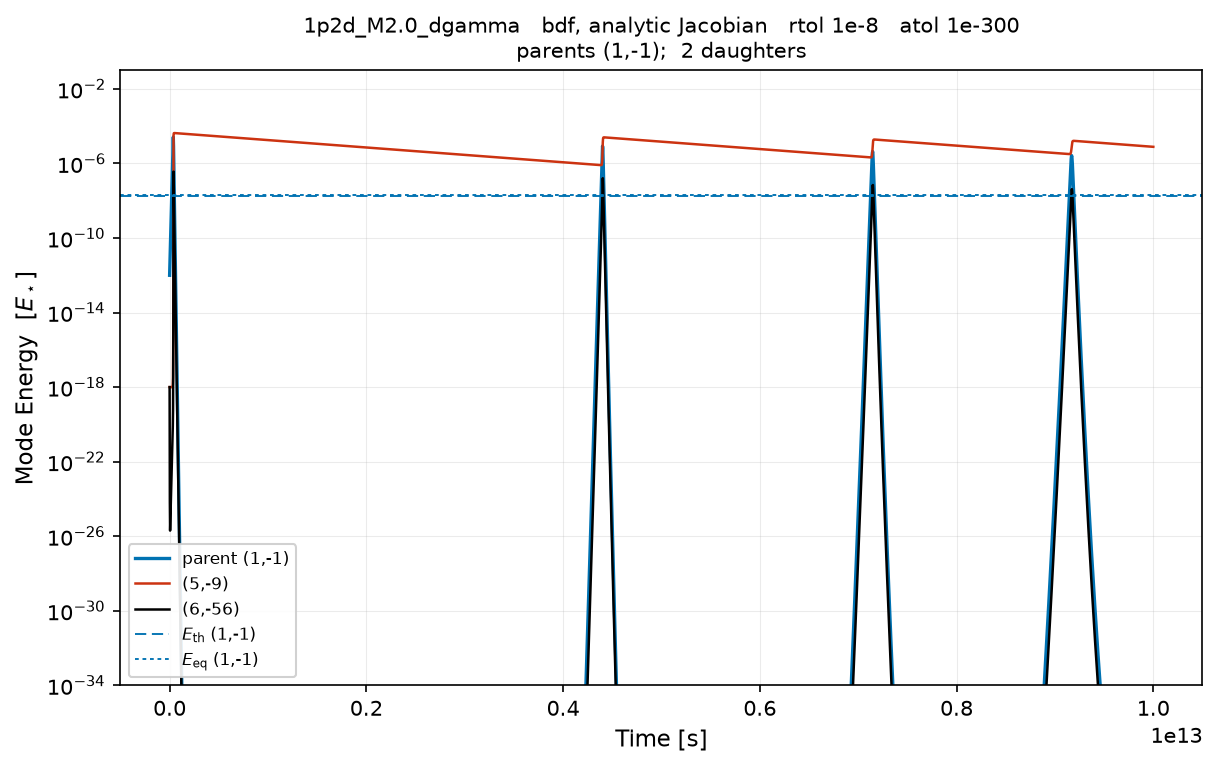
\includegraphics[width=0.21\textwidth,height=0.1323\textwidth]{../plots/bdf/1p2d_M2.0_dgamma/r1e-8_a1e-300.png} & 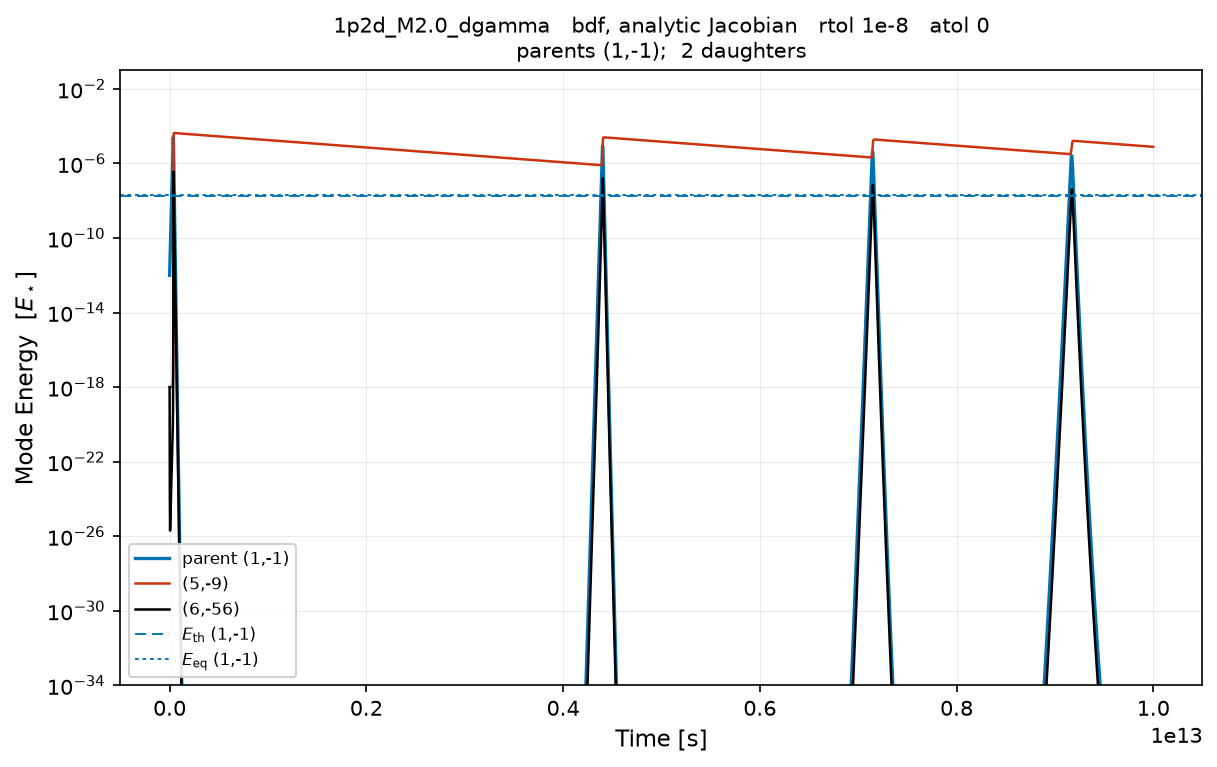
\includegraphics[width=0.21\textwidth,height=0.1323\textwidth]{../plots/bdf/1p2d_M2.0_dgamma/r1e-8_a0.png} \\[-1pt]
 & \parbox[t]{0.21\textwidth}{\centering\scriptsize 14.40\,M steps, 12.8\,s} & \parbox[t]{0.21\textwidth}{\centering\scriptsize 114.97\,M steps, 154.3\,s} & \parbox[t]{0.21\textwidth}{\centering\scriptsize 120.93\,M steps, 140.1\,s} & \parbox[t]{0.21\textwidth}{\centering\scriptsize 120.93\,M steps, 168.2\,s} \\[2pt]
\rotatebox{90}{\parbox{0.1323\textwidth}{\centering\scriptsize\bfseries BDF-Krylov, band full}} & 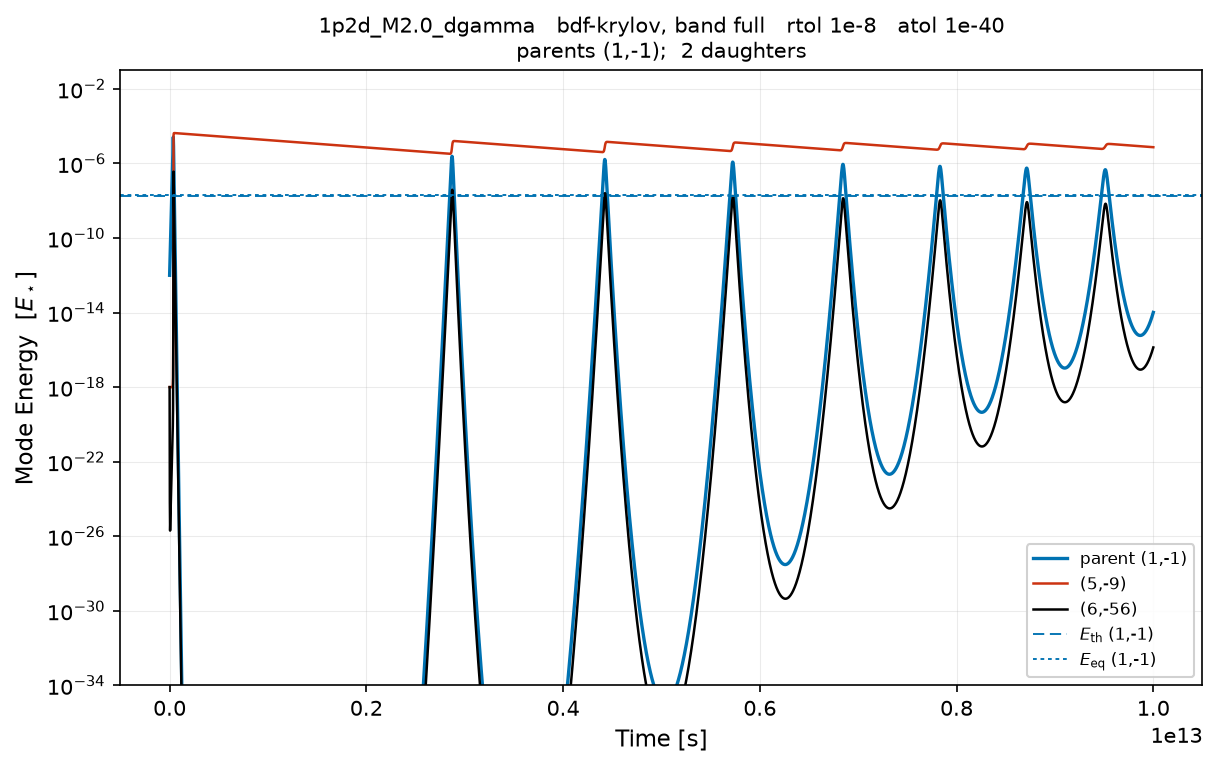
\includegraphics[width=0.21\textwidth,height=0.1323\textwidth]{../plots/krylov_full/1p2d_M2.0_dgamma/r1e-8_a1e-40.png} & 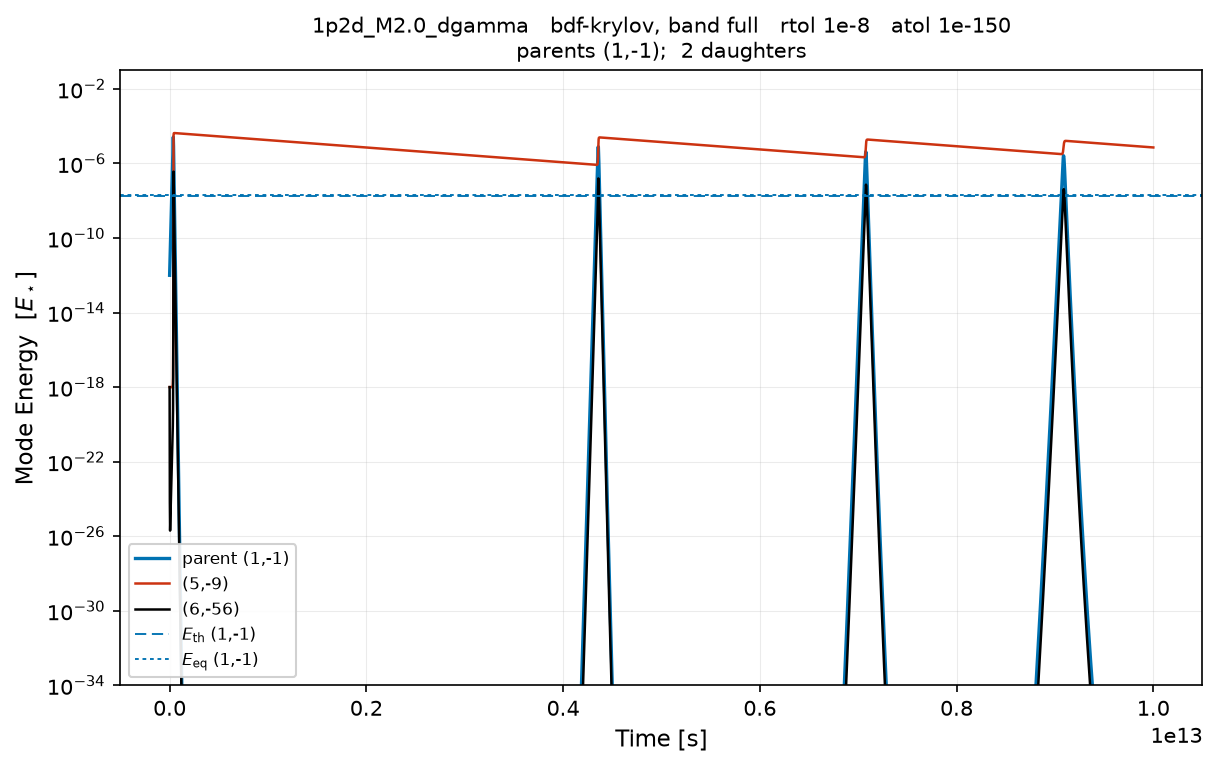
\includegraphics[width=0.21\textwidth,height=0.1323\textwidth]{../plots/krylov_full/1p2d_M2.0_dgamma/r1e-8_a1e-150.png} & 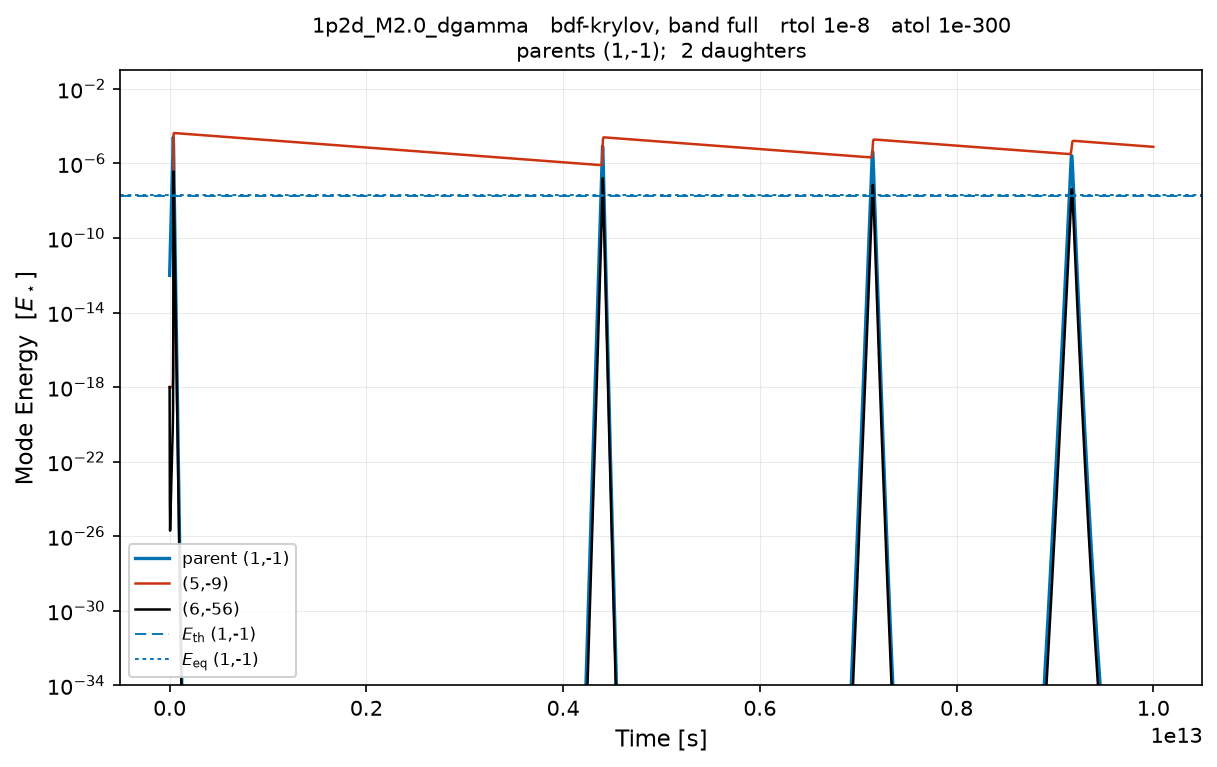
\includegraphics[width=0.21\textwidth,height=0.1323\textwidth]{../plots/krylov_full/1p2d_M2.0_dgamma/r1e-8_a1e-300.png} & 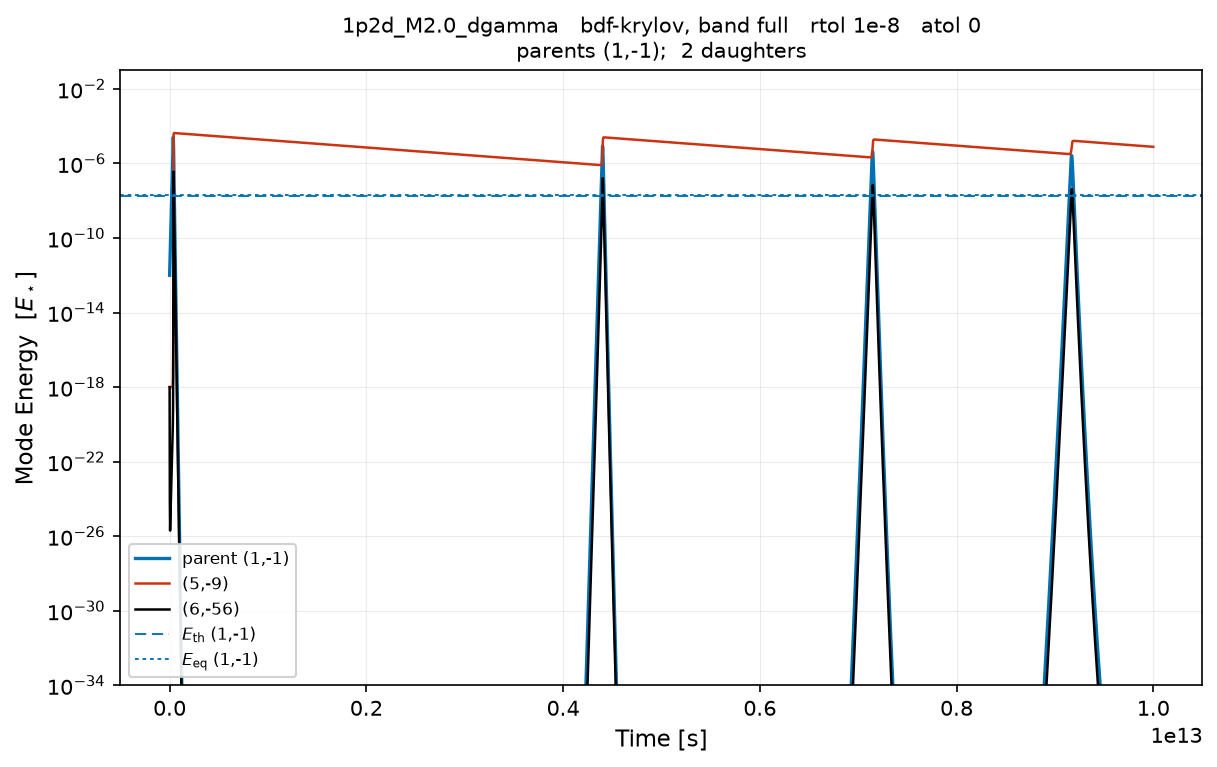
\includegraphics[width=0.21\textwidth,height=0.1323\textwidth]{../plots/krylov_full/1p2d_M2.0_dgamma/r1e-8_a0.png} \\[-1pt]
 & \parbox[t]{0.21\textwidth}{\centering\scriptsize 100.36\,M steps, 124.9\,s} & \parbox[t]{0.21\textwidth}{\centering\scriptsize 111.48\,M steps, 136.5\,s} & \parbox[t]{0.21\textwidth}{\centering\scriptsize 117.07\,M steps, 159.0\,s} & \parbox[t]{0.21\textwidth}{\centering\scriptsize 117.07\,M steps, 176.9\,s} \\[2pt]
\rotatebox{90}{\parbox{0.1323\textwidth}{\centering\scriptsize\bfseries BDF-Krylov, band 3}} & 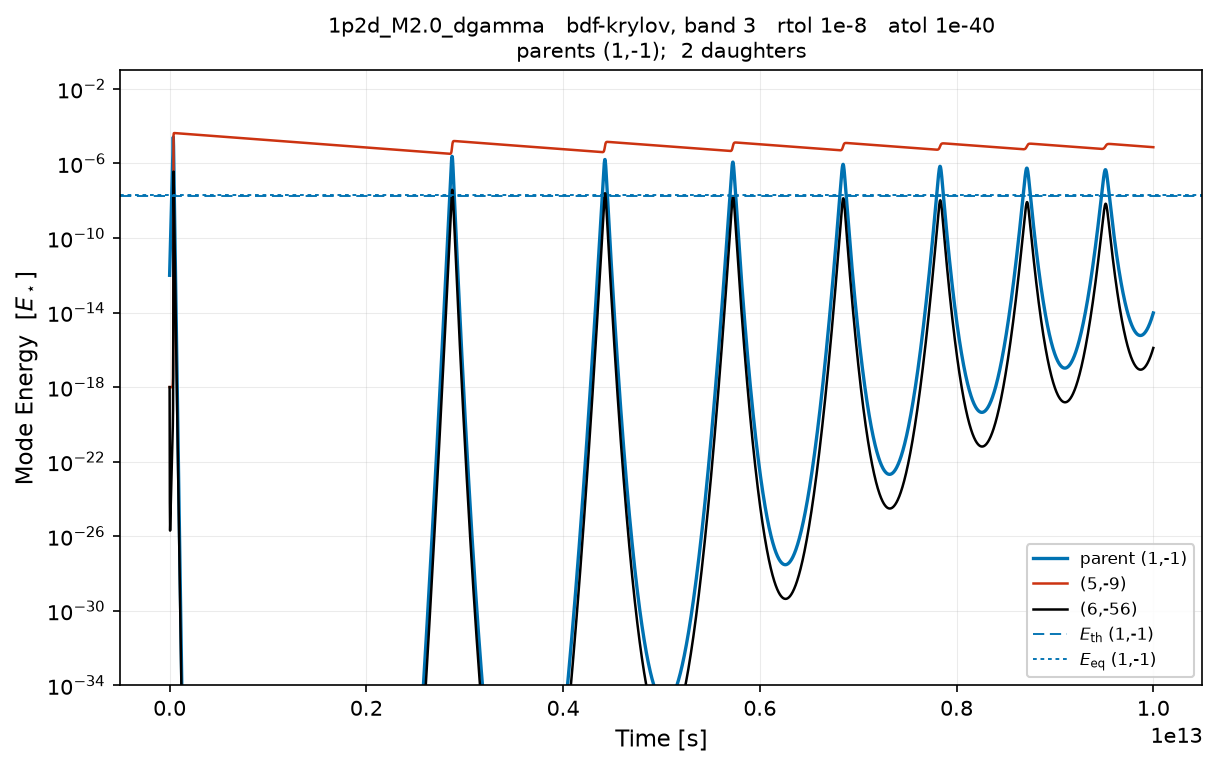
\includegraphics[width=0.21\textwidth,height=0.1323\textwidth]{../plots/krylov_b3/1p2d_M2.0_dgamma/r1e-8_a1e-40.png} & 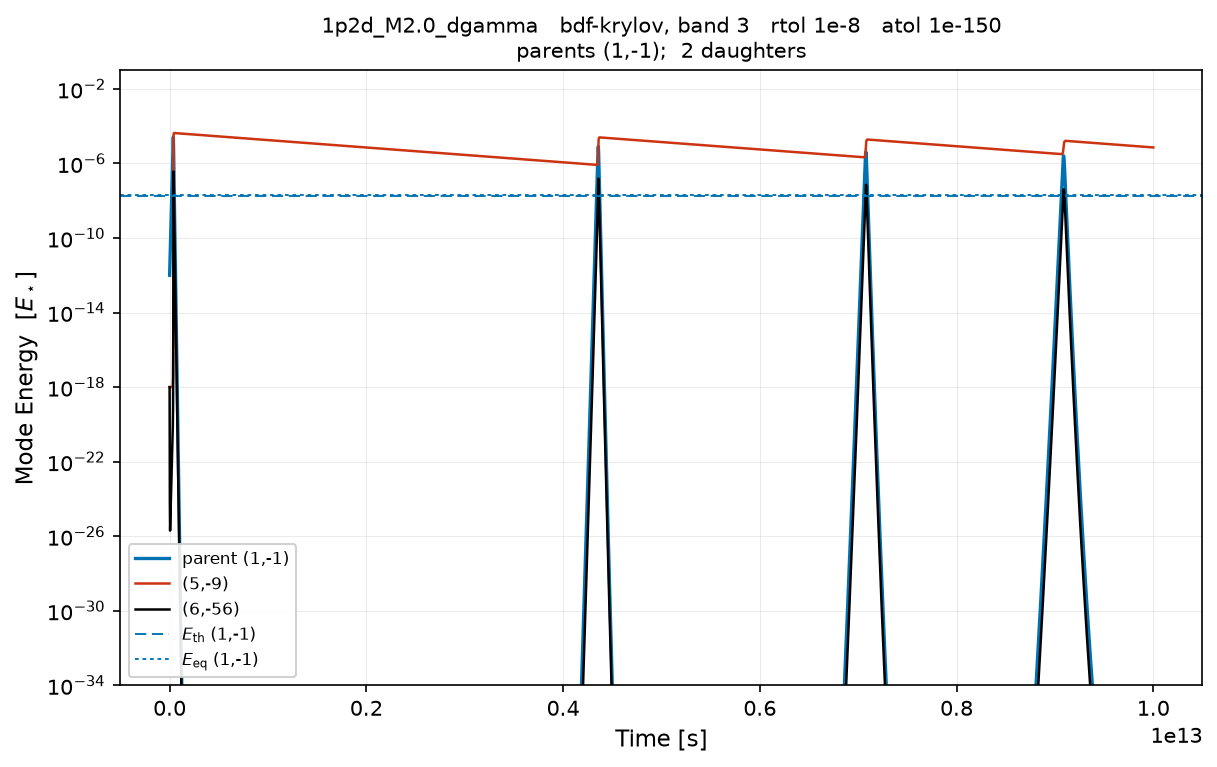
\includegraphics[width=0.21\textwidth,height=0.1323\textwidth]{../plots/krylov_b3/1p2d_M2.0_dgamma/r1e-8_a1e-150.png} & 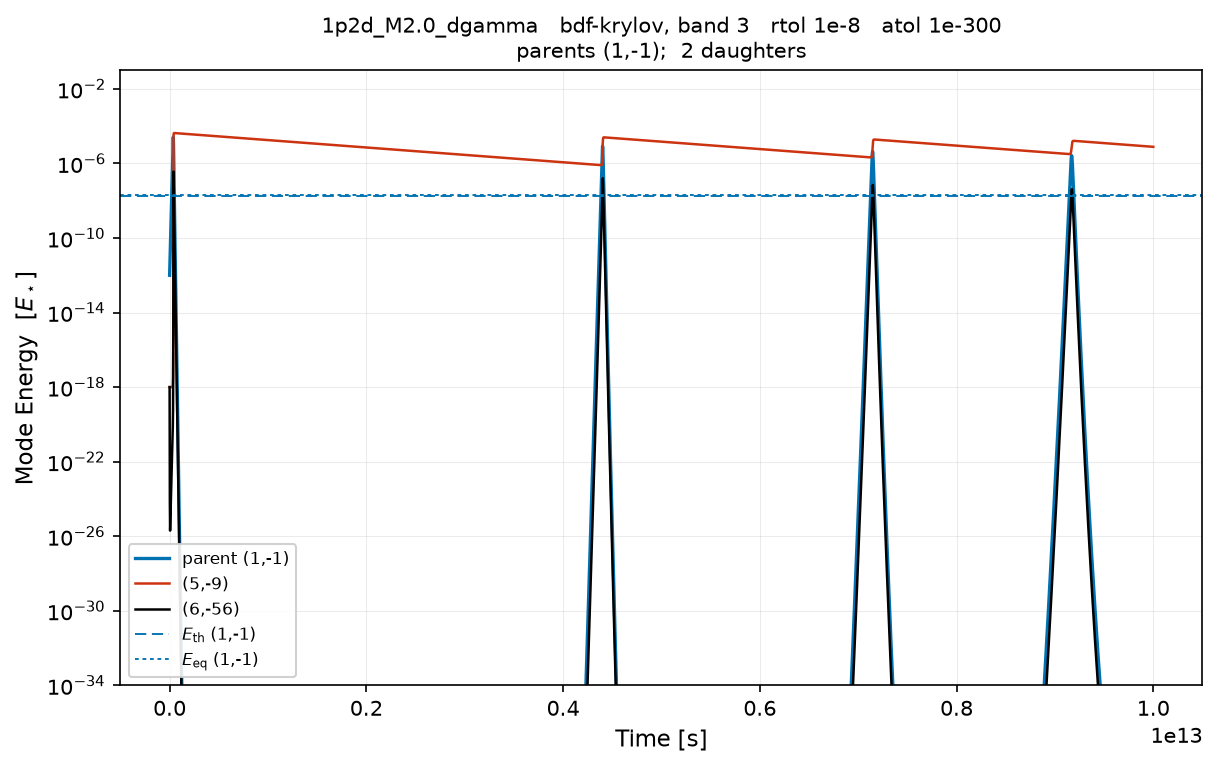
\includegraphics[width=0.21\textwidth,height=0.1323\textwidth]{../plots/krylov_b3/1p2d_M2.0_dgamma/r1e-8_a1e-300.png} & 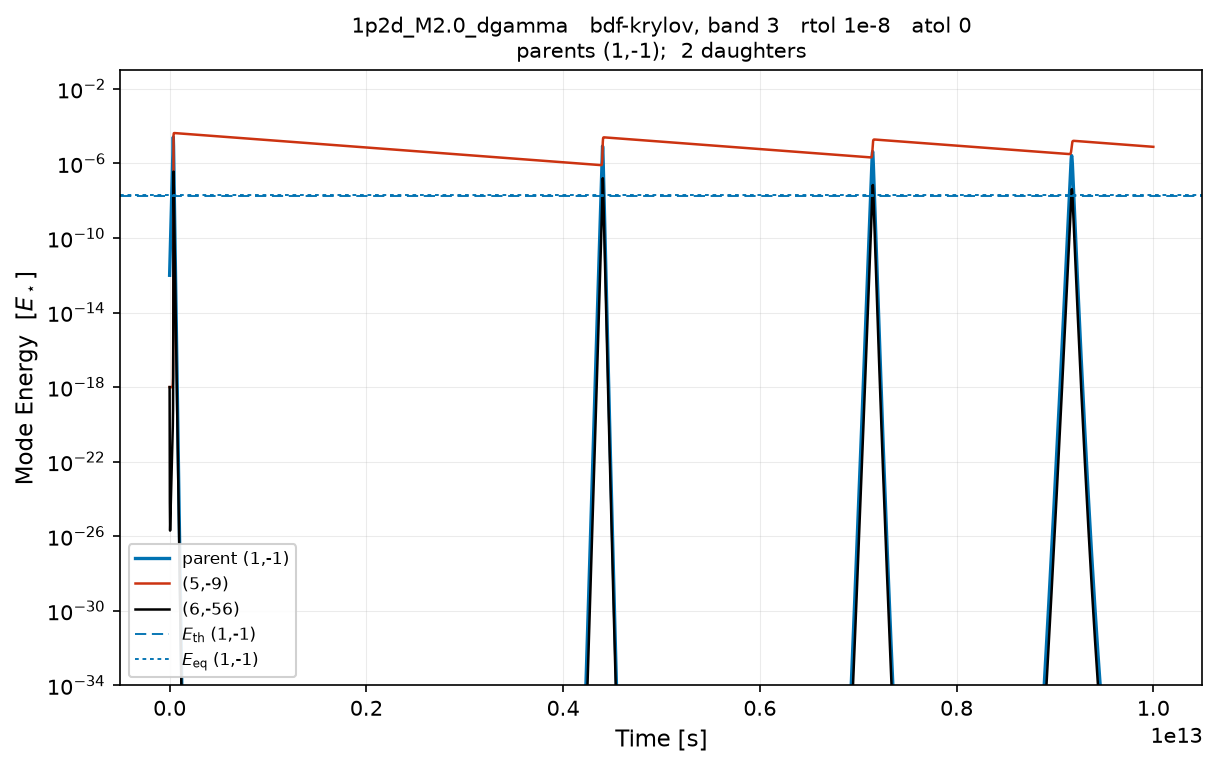
\includegraphics[width=0.21\textwidth,height=0.1323\textwidth]{../plots/krylov_b3/1p2d_M2.0_dgamma/r1e-8_a0.png} \\[-1pt]
 & \parbox[t]{0.21\textwidth}{\centering\scriptsize 99.14\,M steps, 140.6\,s} & \parbox[t]{0.21\textwidth}{\centering\scriptsize 110.16\,M steps, 156.8\,s} & \parbox[t]{0.21\textwidth}{\centering\scriptsize 115.72\,M steps, 155.0\,s} & \parbox[t]{0.21\textwidth}{\centering\scriptsize 115.72\,M steps, 204.6\,s} \\[2pt]
\rotatebox{90}{\parbox{0.1323\textwidth}{\centering\scriptsize\bfseries Adams, fixed point}} & 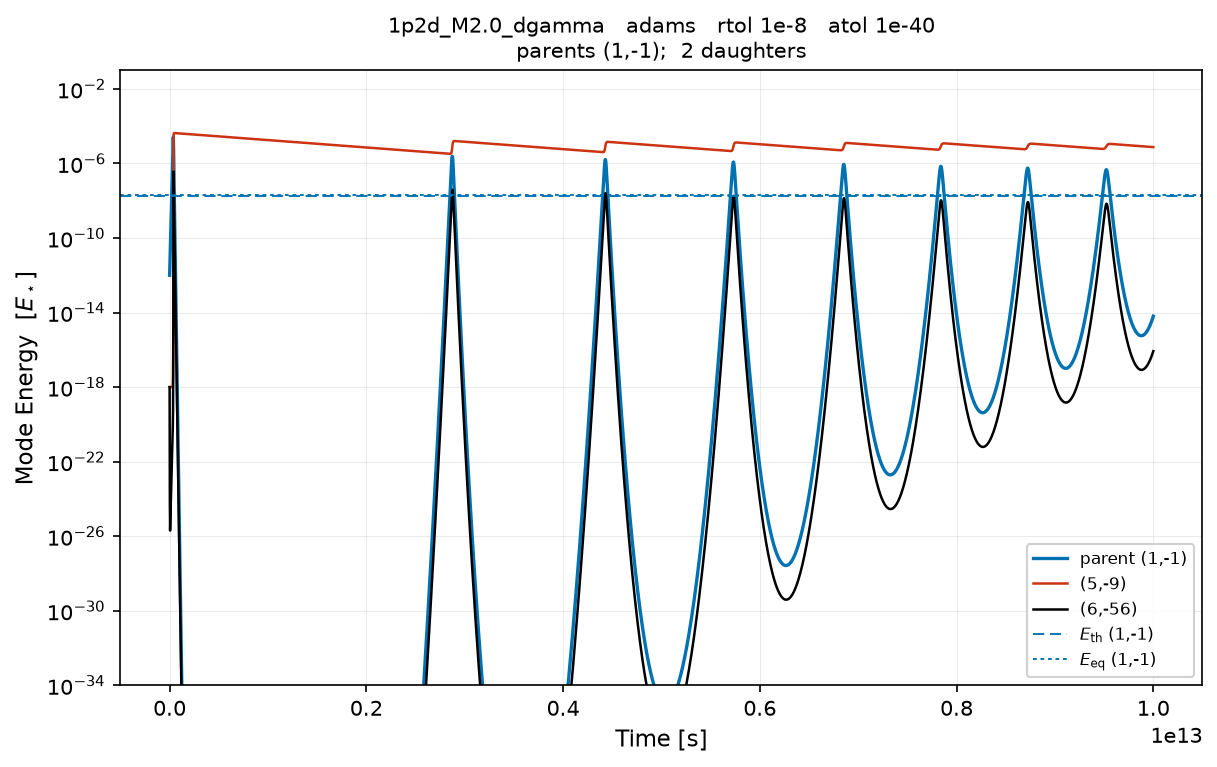
\includegraphics[width=0.21\textwidth,height=0.1323\textwidth]{../plots/adams/1p2d_M2.0_dgamma/r1e-8_a1e-40.png} & 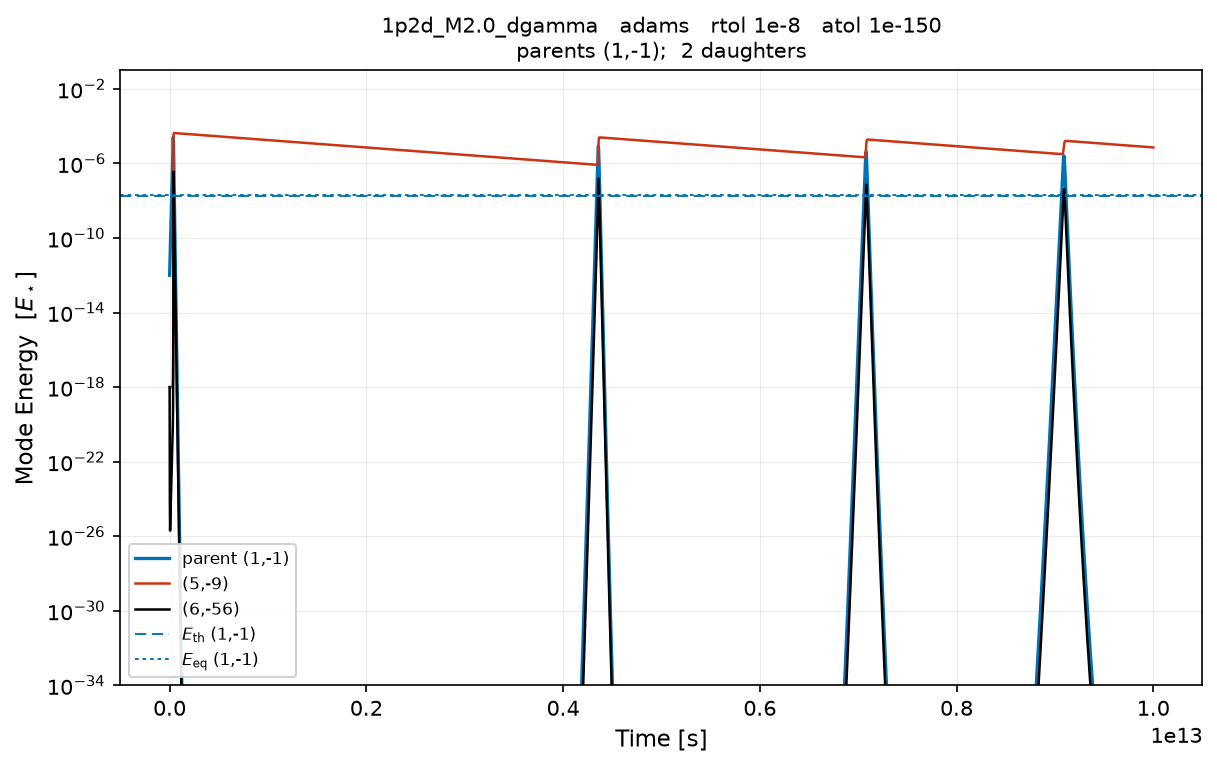
\includegraphics[width=0.21\textwidth,height=0.1323\textwidth]{../plots/adams/1p2d_M2.0_dgamma/r1e-8_a1e-150.png} & 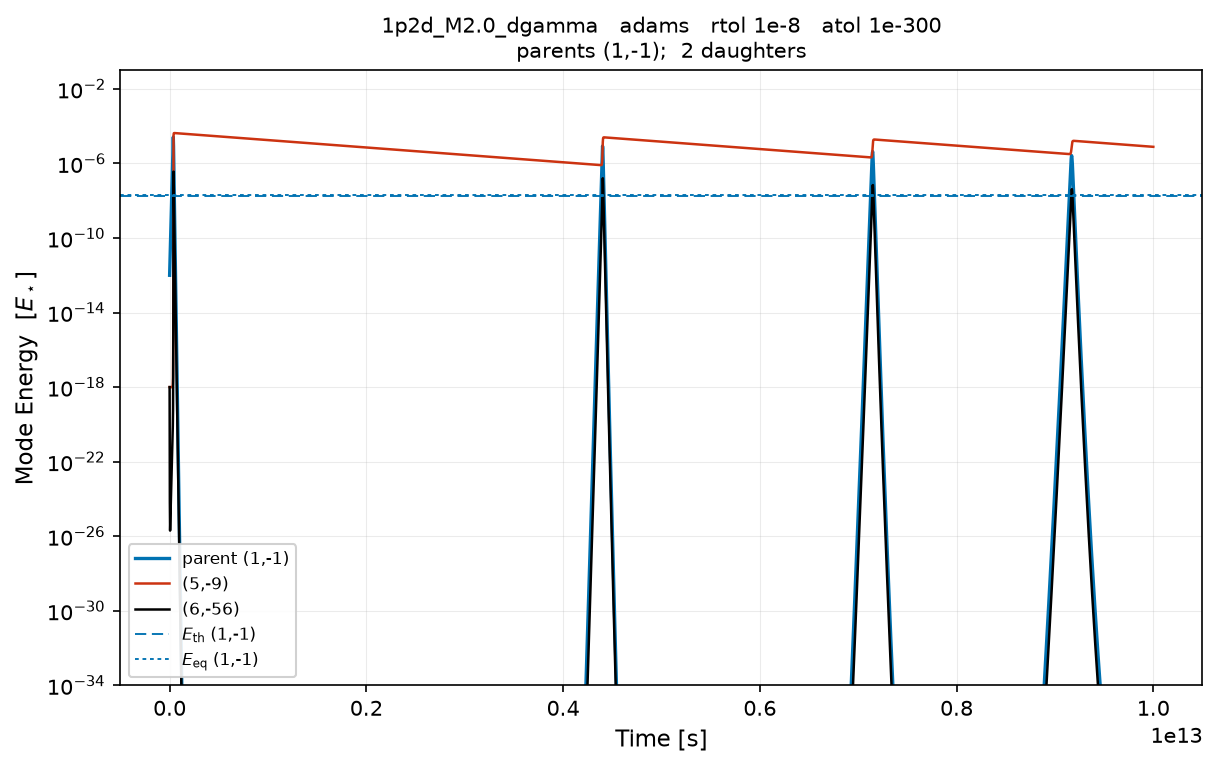
\includegraphics[width=0.21\textwidth,height=0.1323\textwidth]{../plots/adams/1p2d_M2.0_dgamma/r1e-8_a1e-300.png} & 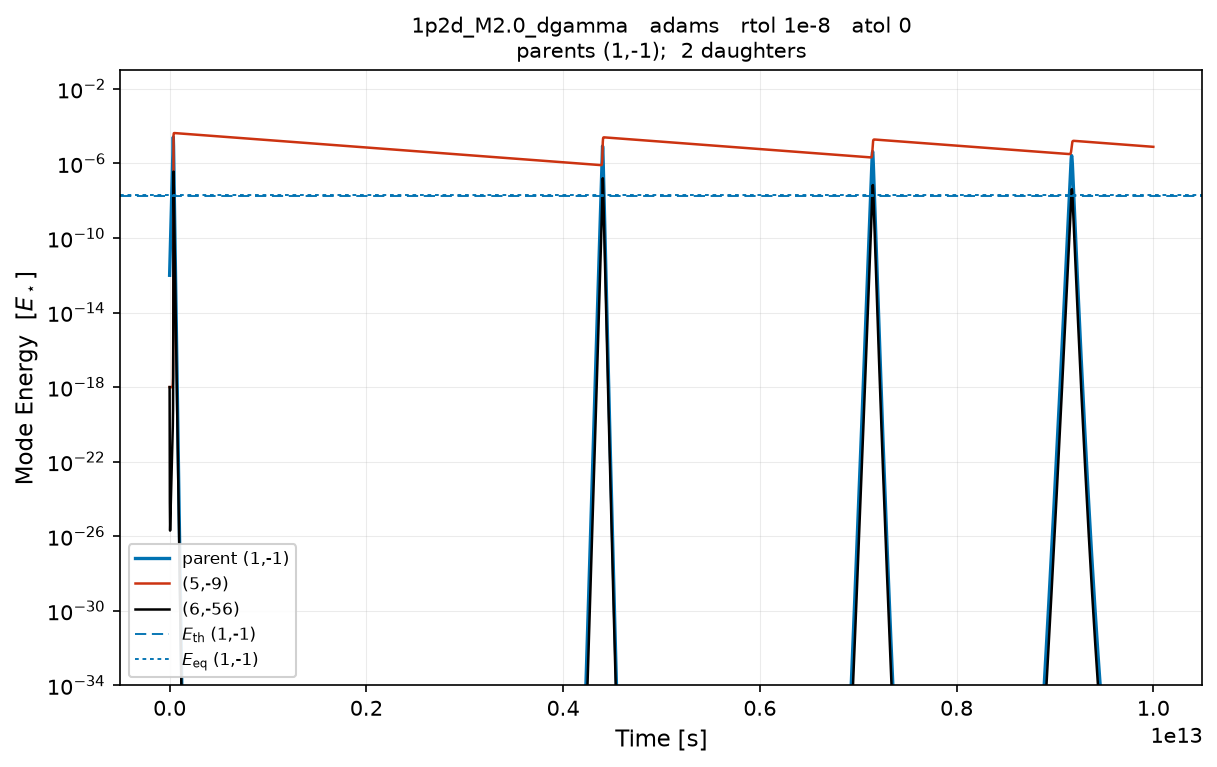
\includegraphics[width=0.21\textwidth,height=0.1323\textwidth]{../plots/adams/1p2d_M2.0_dgamma/r1e-8_a0.png} \\[-1pt]
 & \parbox[t]{0.21\textwidth}{\centering\scriptsize 43.17\,M steps, 39.5\,s} & \parbox[t]{0.21\textwidth}{\centering\scriptsize 47.54\,M steps, 45.3\,s} & \parbox[t]{0.21\textwidth}{\centering\scriptsize 48.28\,M steps, 54.4\,s} & \parbox[t]{0.21\textwidth}{\centering\scriptsize 48.28\,M steps, 43.5\,s} \\[2pt]
\end{tabular}\par}
\par\noindent{\scriptsize\setlength\tabcolsep{3.5pt}\renewcommand\arraystretch{0.92}
\begin{tabular}{@{}llllrrrrrrr@{}}
\toprule
integrator & atol & stop & $t_{\rm stop}$ [s] & steps & rejected & RHS & Jac. & NL it. & lin. it. & wall [s] \\
\midrule
rk8pd & $10^{-40}$ & end & $1.00\times10^{13}$ & 6.61\,M & 575.7\,k & 85.89\,M & -- & -- & -- & 9.5 \\
 & $10^{-150}$ & end & $1.00\times10^{13}$ & 8.24\,M & 937.9\,k & 107.11\,M & -- & -- & -- & 15.6 \\
 & $10^{-300}$ & end & $1.00\times10^{13}$ & 9.26\,M & 1.04\,M & 120.43\,M & -- & -- & -- & 13.5 \\
 & $0$ & end & $1.00\times10^{13}$ & 9.26\,M & 1.04\,M & 120.43\,M & -- & -- & -- & 20.4 \\
\addlinespace[2pt]
BDF, dense analytic Jacobian & $10^{-40}$ & end & $1.00\times10^{13}$ & 14.40\,M & 215.6\,k & 16.26\,M & 378.7\,k & 16.26\,M & -- & 12.8 \\
 & $10^{-150}$ & end & $1.00\times10^{13}$ & 114.97\,M & 655.1\,k & 121.60\,M & 1.93\,M & 121.59\,M & -- & 154.3 \\
 & $10^{-300}$ & end & $1.00\times10^{13}$ & 120.93\,M & 719.2\,k & 127.92\,M & 2.03\,M & 127.91\,M & -- & 140.1 \\
 & $0$ & end & $1.00\times10^{13}$ & 120.93\,M & 719.2\,k & 127.92\,M & 2.03\,M & 127.91\,M & -- & 168.2 \\
\addlinespace[2pt]
BDF-Krylov, band full & $10^{-40}$ & end & $1.00\times10^{13}$ & 100.36\,M & 648.8\,k & 225.12\,M & 1.69\,M & 107.09\,M & 107.90\,M & 124.9 \\
 & $10^{-150}$ & end & $1.00\times10^{13}$ & 111.48\,M & 738.1\,k & 246.46\,M & 1.87\,M & 118.93\,M & 116.29\,M & 136.5 \\
 & $10^{-300}$ & end & $1.00\times10^{13}$ & 117.07\,M & 821.6\,k & 257.00\,M & 1.97\,M & 124.94\,M & 120.27\,M & 159.0 \\
 & $0$ & end & $1.00\times10^{13}$ & 117.07\,M & 821.6\,k & 257.00\,M & 1.97\,M & 124.94\,M & 120.27\,M & 176.9 \\
\addlinespace[2pt]
BDF-Krylov, band 3 & $10^{-40}$ & end & $1.00\times10^{13}$ & 99.14\,M & 679.3\,k & 223.80\,M & 1.66\,M & 106.16\,M & 107.65\,M & 140.6 \\
 & $10^{-150}$ & end & $1.00\times10^{13}$ & 110.16\,M & 777.2\,k & 244.85\,M & 1.85\,M & 117.94\,M & 115.81\,M & 156.8 \\
 & $10^{-300}$ & end & $1.00\times10^{13}$ & 115.72\,M & 853.2\,k & 255.64\,M & 1.94\,M & 123.92\,M & 120.06\,M & 155.0 \\
 & $0$ & end & $1.00\times10^{13}$ & 115.72\,M & 853.2\,k & 255.64\,M & 1.94\,M & 123.92\,M & 120.06\,M & 204.6 \\
\addlinespace[2pt]
Adams, fixed point & $10^{-40}$ & end & $1.00\times10^{13}$ & 43.17\,M & 1.65\,M & 61.88\,M & -- & 61.88\,M & -- & 39.5 \\
 & $10^{-150}$ & end & $1.00\times10^{13}$ & 47.54\,M & 2.13\,M & 69.35\,M & -- & 69.35\,M & -- & 45.3 \\
 & $10^{-300}$ & end & $1.00\times10^{13}$ & 48.28\,M & 2.32\,M & 68.68\,M & -- & 68.68\,M & -- & 54.4 \\
 & $0$ & end & $1.00\times10^{13}$ & 48.28\,M & 2.32\,M & 68.68\,M & -- & 68.68\,M & -- & 43.5 \\
\bottomrule
\end{tabular}}

\clearpage
\subsection{\texttt{1p4d\_M1.7\_eth}}\label{net:1p4d_M1.7_eth}
\noindent\begin{minipage}[t]{0.43\textwidth}\vspace{0pt}\footnotesize
\begin{tabular}{@{}rrlrr@{}}
\toprule
id & gen & $(\ell,n)$ & $\omega$ [rad\,s$^{-1}$] & $\gamma$ [s$^{-1}$] \\
\midrule
0 & 0 & (1,+1) & $1.402\times10^{-3}$ & $-1.150\times10^{-10}$ \\
1 & 1 & (6,$-$6) & $1.070\times10^{-3}$ & $4.184\times10^{-13}$ \\
2 & 1 & (7,$-$27) & $3.326\times10^{-4}$ & $8.612\times10^{-10}$ \\
3 & 1 & (5,$-$14) & $4.541\times10^{-4}$ & $7.998\times10^{-12}$ \\
4 & 1 & (6,$-$7) & $9.483\times10^{-4}$ & $7.855\times10^{-13}$ \\
\bottomrule
\end{tabular}
\end{minipage}\hfill
\begin{minipage}[t]{0.55\textwidth}\vspace{0pt}\footnotesize
\textbf{Model} \texttt{dsct\_M1.7\_T7750}, rule eth, $N=4$, cut 0.15,
closure 0.005; 5 modes, 2 triplet(s).\\[2pt]
\textbf{Selecting pairs}\\ (1,+1) $\to$ (6,$-$6) + (7,$-$27): $\Delta/\omega_a=-3.98\times10^{-5}$, $\kappa=+0.107$, $E_{\rm th}=9.22\times10^{-11}$, $E_{\rm eq}=1.23\times10^{-10}$\\
(1,+1) $\to$ (5,$-$14) + (6,$-$7): $\Delta/\omega_a=1.51\times10^{-5}$, $\kappa=+0.369$, $E_{\rm th}=1.57\times10^{-10}$, no $E_{\rm eq}$\\[2pt]
Runaway near $3\times10^{11}$\,s.
\end{minipage}

\par\smallskip{\centering\begin{tabular}{@{}c@{\hspace{2pt}}c@{\hspace{2pt}}c@{\hspace{2pt}}c@{\hspace{2pt}}c@{}}
 & \small atol $10^{-40}$ & \small atol $10^{-150}$ & \small atol $10^{-300}$ & \small atol $0$ \\[1pt]
\rotatebox{90}{\parbox{0.1323\textwidth}{\centering\scriptsize\bfseries rk8pd}} & 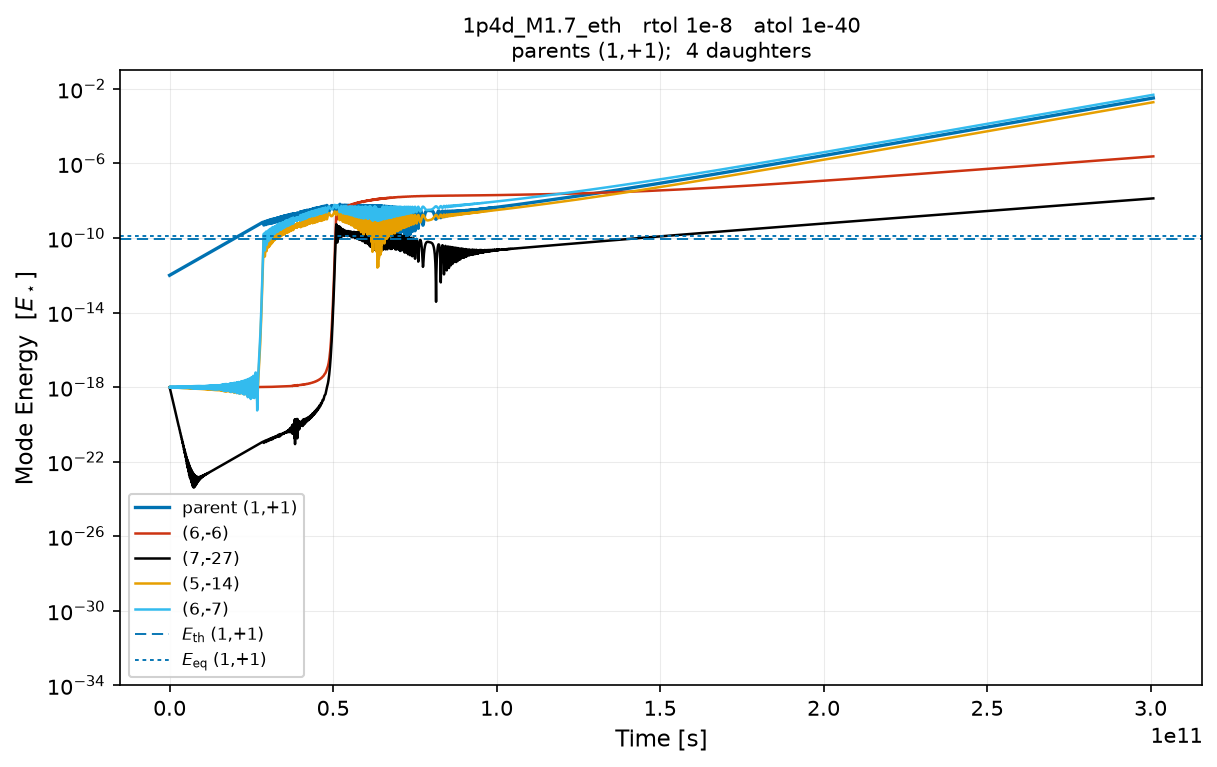
\includegraphics[width=0.21\textwidth,height=0.1323\textwidth]{../plots/rk8pd/1p4d_M1.7_eth/r1e-8_a1e-40.png} & 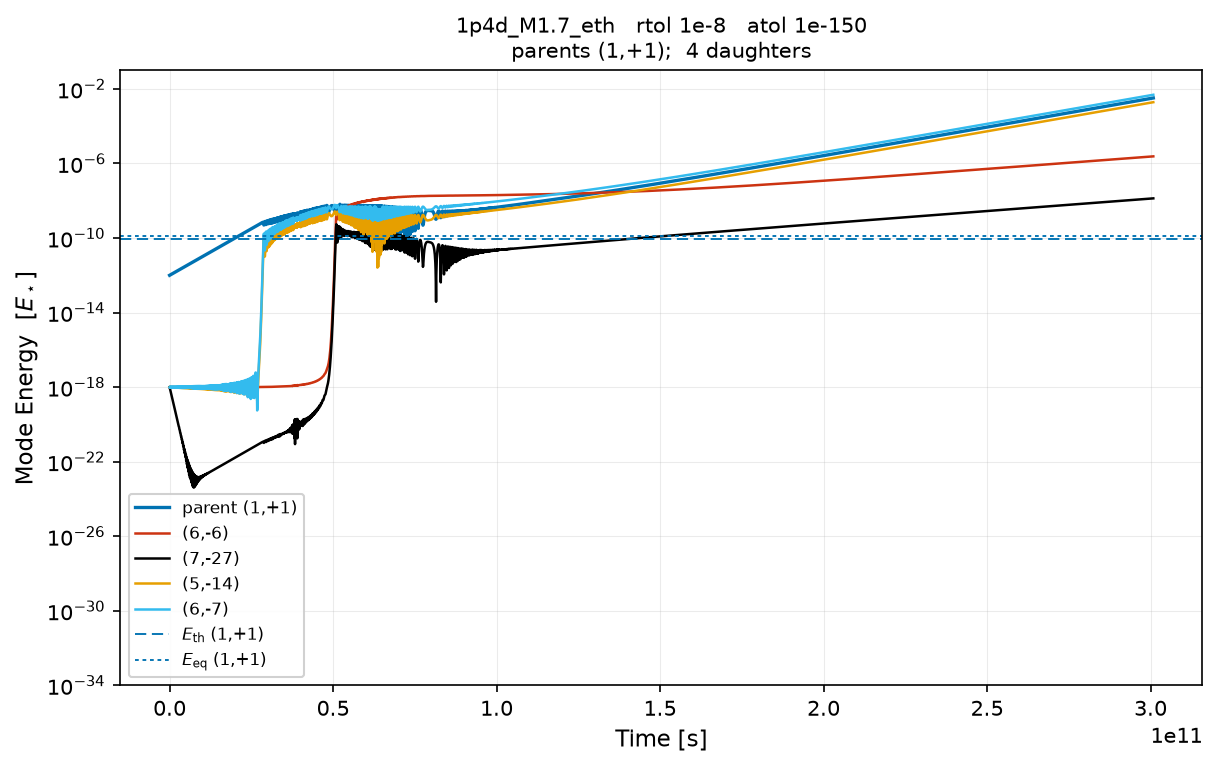
\includegraphics[width=0.21\textwidth,height=0.1323\textwidth]{../plots/rk8pd/1p4d_M1.7_eth/r1e-8_a1e-150.png} & 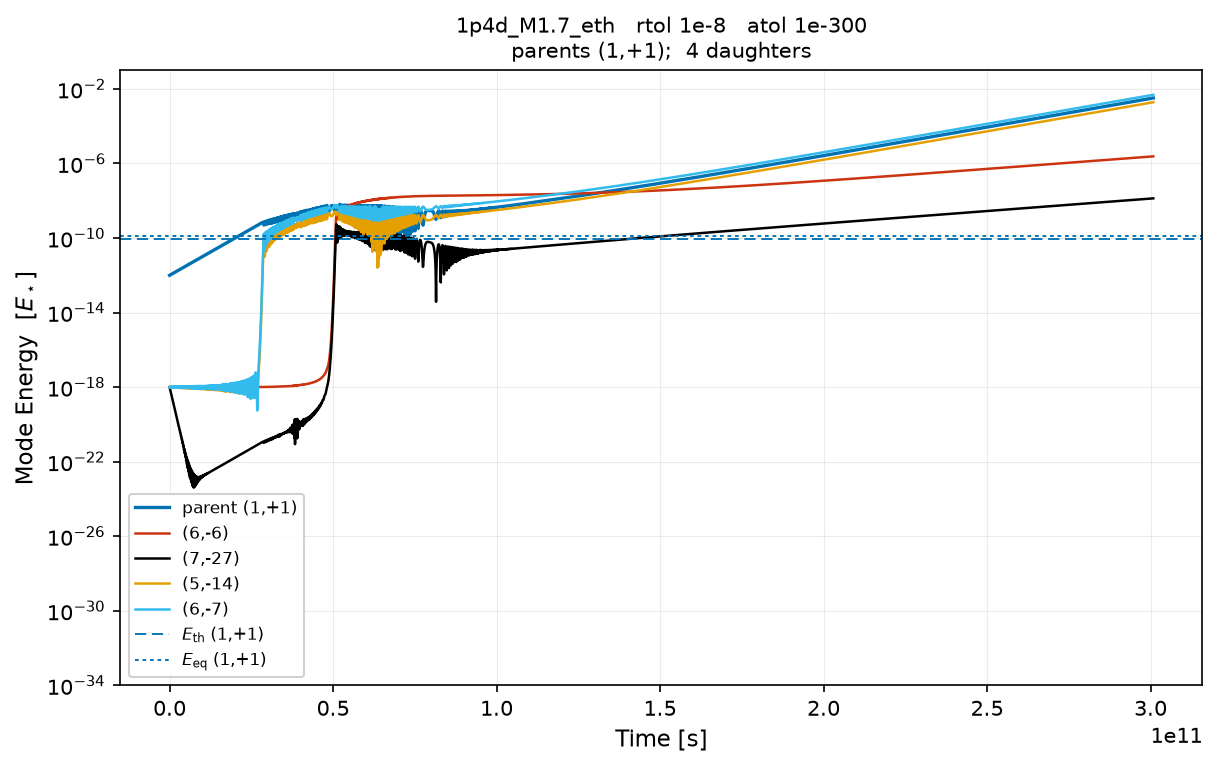
\includegraphics[width=0.21\textwidth,height=0.1323\textwidth]{../plots/rk8pd/1p4d_M1.7_eth/r1e-8_a1e-300.png} & 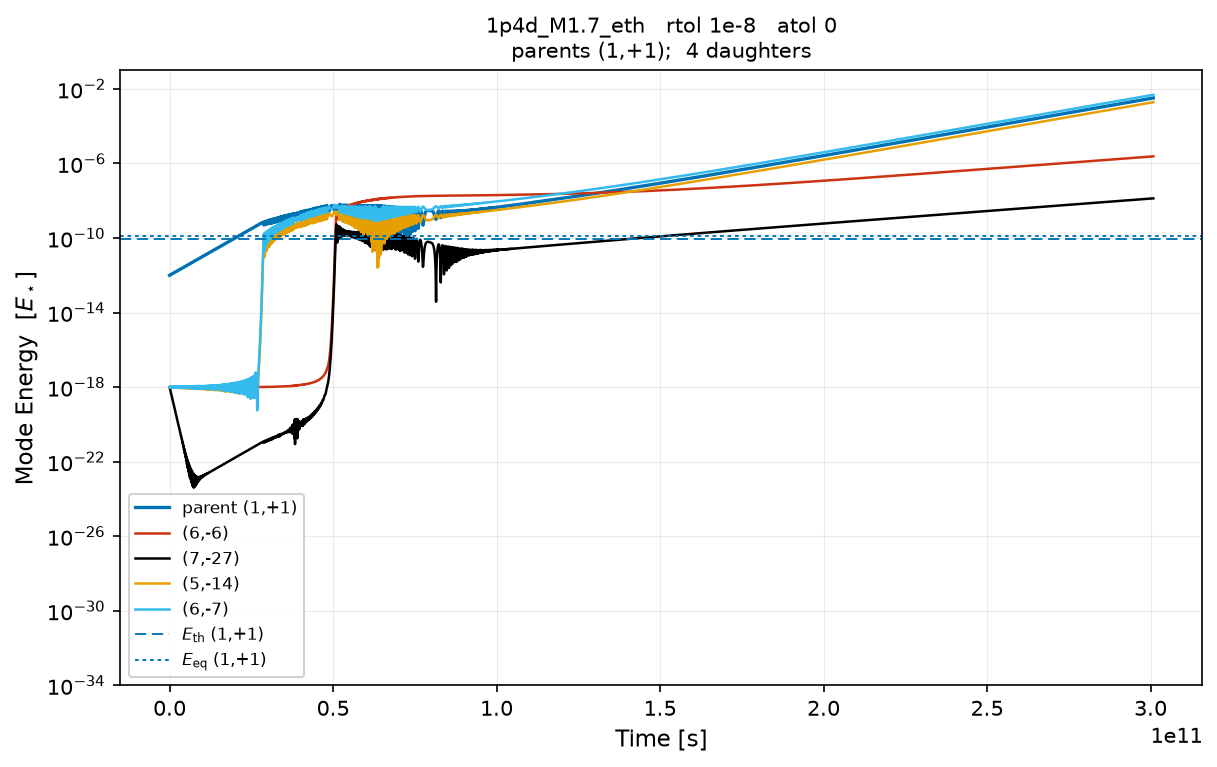
\includegraphics[width=0.21\textwidth,height=0.1323\textwidth]{../plots/rk8pd/1p4d_M1.7_eth/r1e-8_a0.png} \\[-1pt]
 & \parbox[t]{0.21\textwidth}{\centering\scriptsize 7.58\,M steps, 19.8\,s, runaway} & \parbox[t]{0.21\textwidth}{\centering\scriptsize 7.58\,M steps, 17.7\,s, runaway} & \parbox[t]{0.21\textwidth}{\centering\scriptsize 7.58\,M steps, 18.4\,s, runaway} & \parbox[t]{0.21\textwidth}{\centering\scriptsize 7.58\,M steps, 19.8\,s, runaway} \\[2pt]
\rotatebox{90}{\parbox{0.1323\textwidth}{\centering\scriptsize\bfseries BDF, dense analytic Jacobian}} & 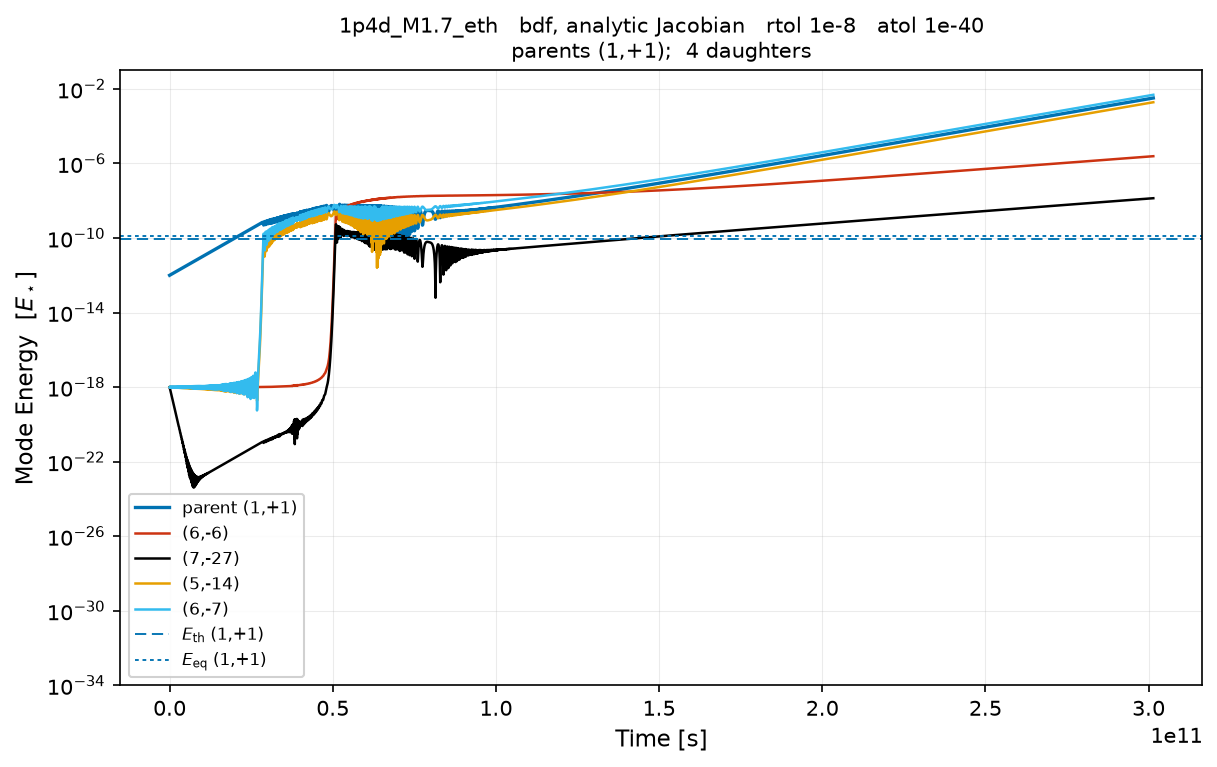
\includegraphics[width=0.21\textwidth,height=0.1323\textwidth]{../plots/bdf/1p4d_M1.7_eth/r1e-8_a1e-40.png} & 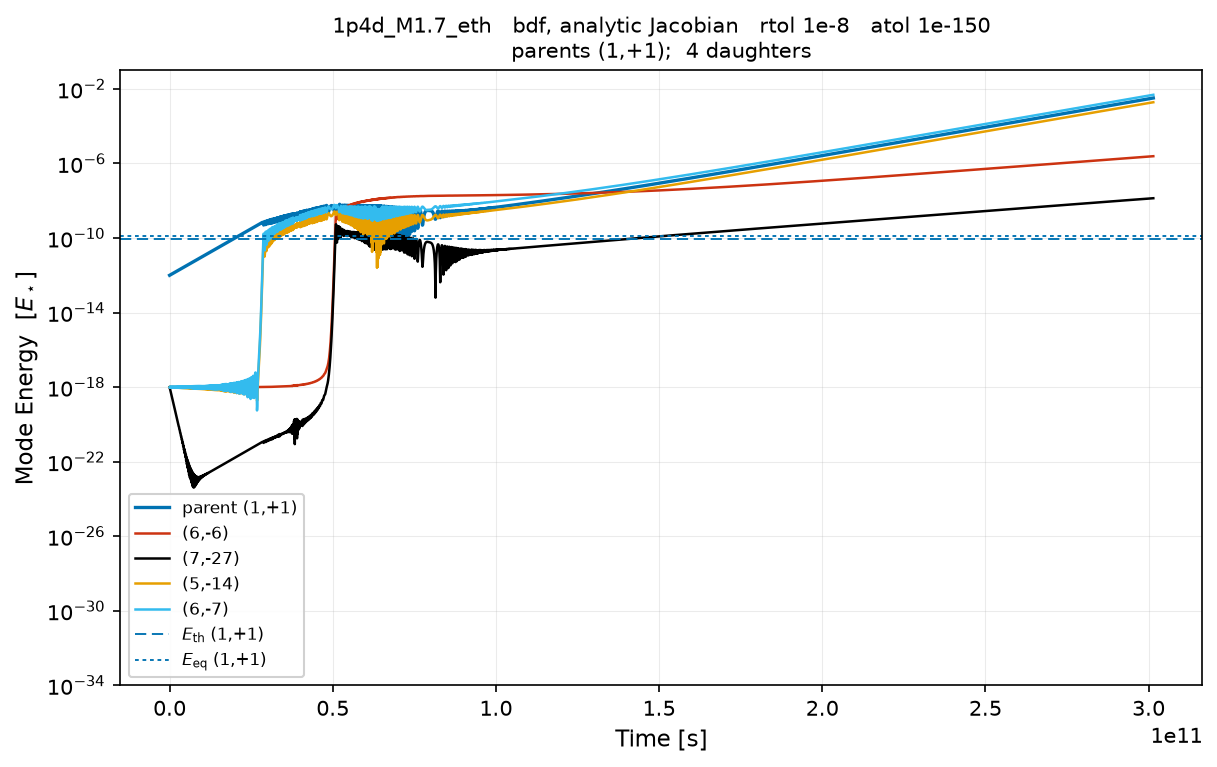
\includegraphics[width=0.21\textwidth,height=0.1323\textwidth]{../plots/bdf/1p4d_M1.7_eth/r1e-8_a1e-150.png} & 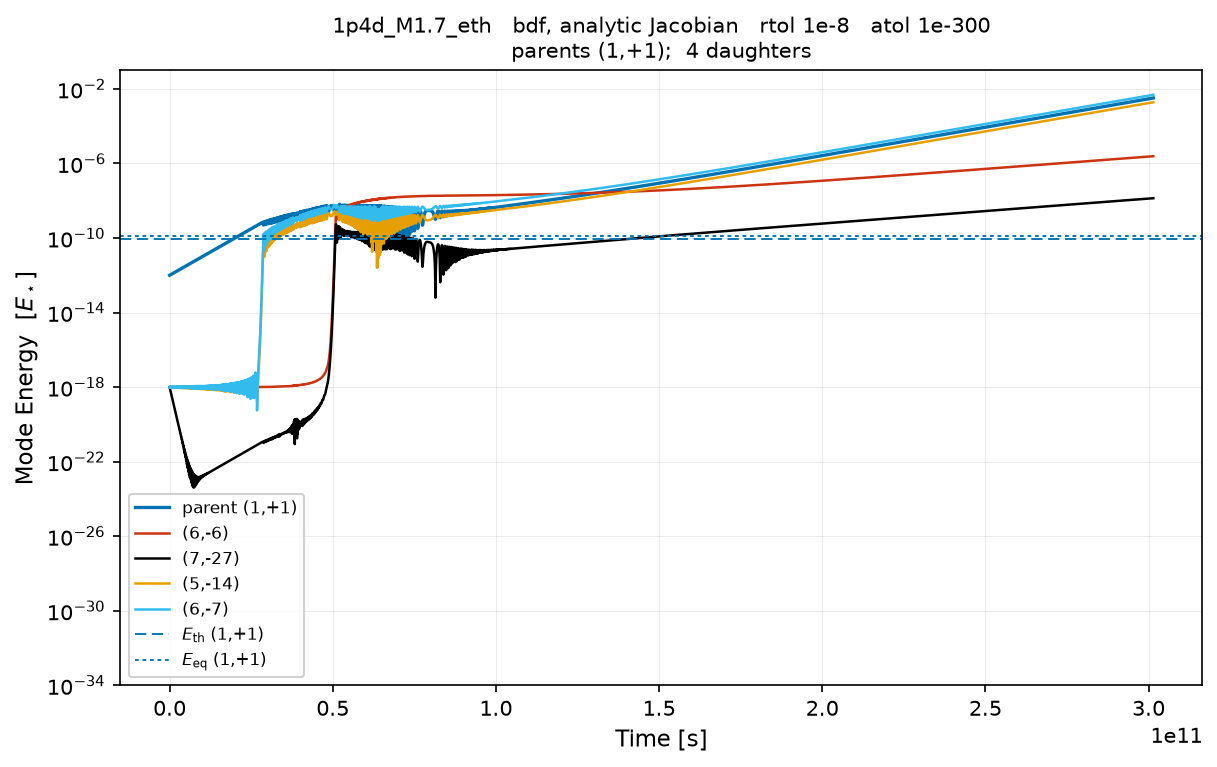
\includegraphics[width=0.21\textwidth,height=0.1323\textwidth]{../plots/bdf/1p4d_M1.7_eth/r1e-8_a1e-300.png} & 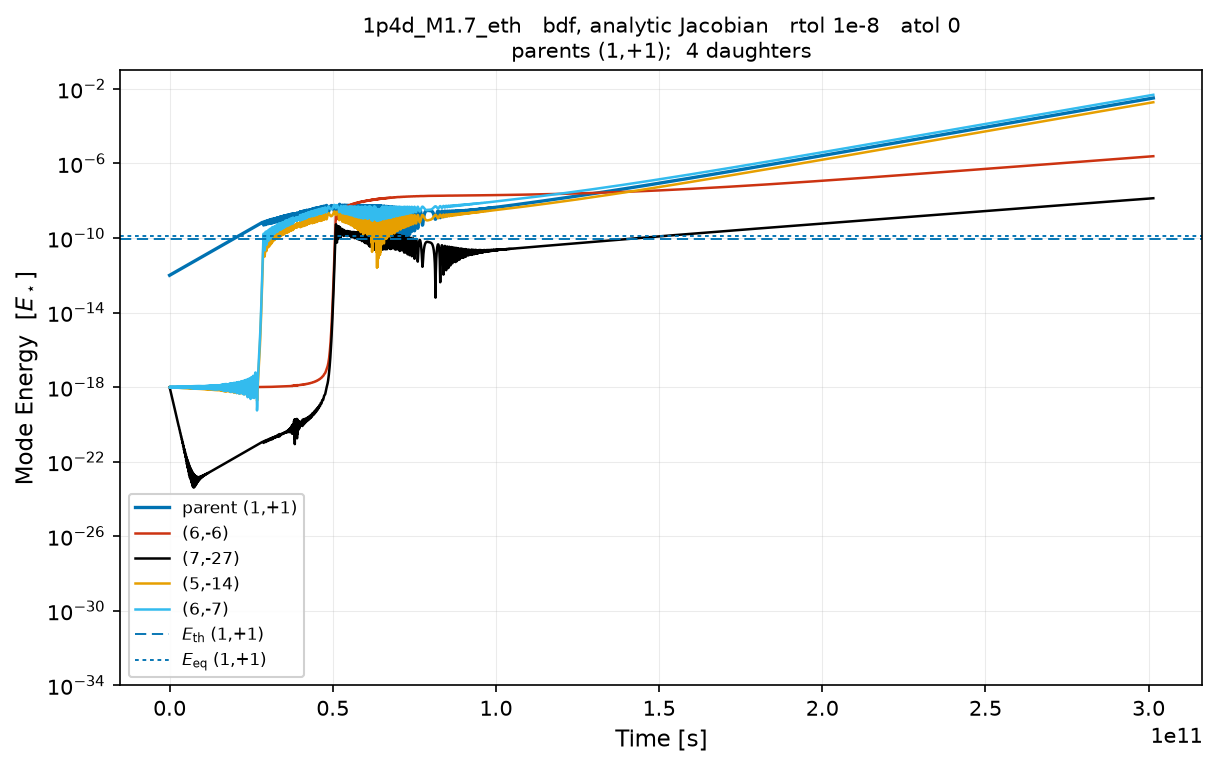
\includegraphics[width=0.21\textwidth,height=0.1323\textwidth]{../plots/bdf/1p4d_M1.7_eth/r1e-8_a0.png} \\[-1pt]
 & \parbox[t]{0.21\textwidth}{\centering\scriptsize 72.42\,M steps, 74.9\,s, runaway} & \parbox[t]{0.21\textwidth}{\centering\scriptsize 72.41\,M steps, 74.4\,s, runaway} & \parbox[t]{0.21\textwidth}{\centering\scriptsize 72.41\,M steps, 122.1\,s, runaway} & \parbox[t]{0.21\textwidth}{\centering\scriptsize 72.41\,M steps, 90.0\,s, runaway} \\[2pt]
\rotatebox{90}{\parbox{0.1323\textwidth}{\centering\scriptsize\bfseries BDF-Krylov, band full}} & 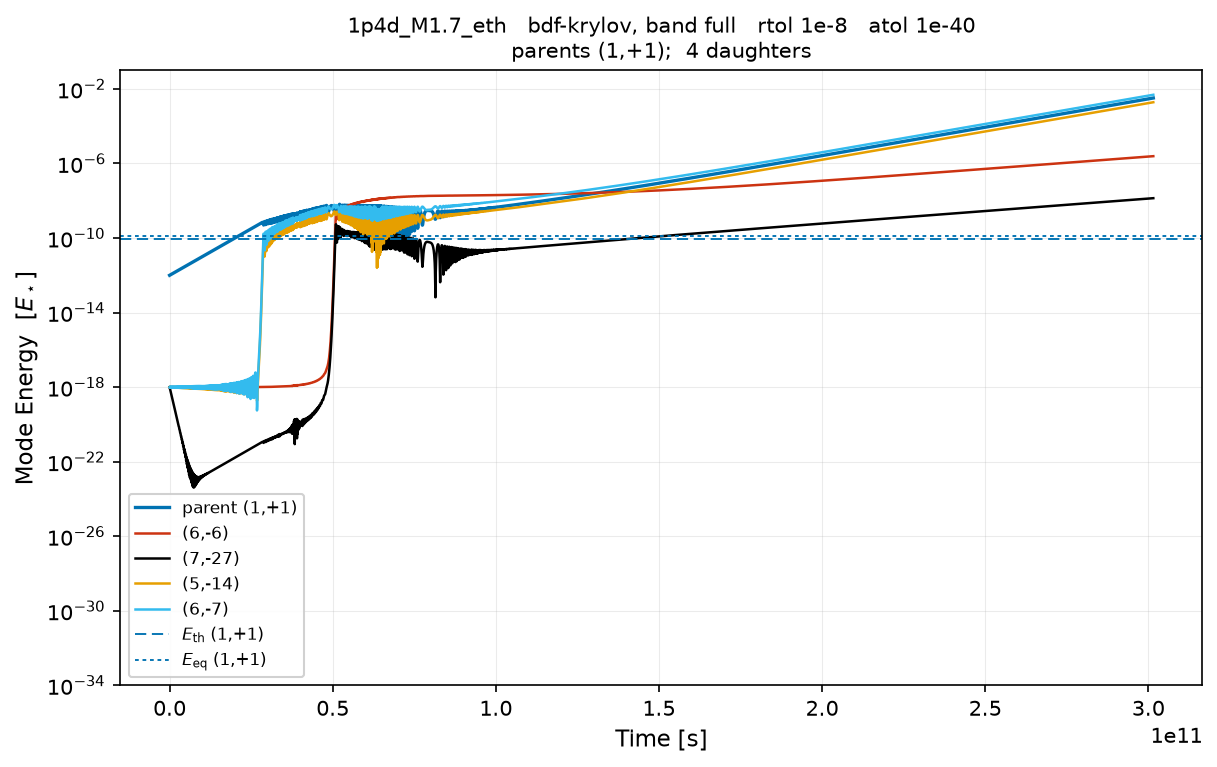
\includegraphics[width=0.21\textwidth,height=0.1323\textwidth]{../plots/krylov_full/1p4d_M1.7_eth/r1e-8_a1e-40.png} & 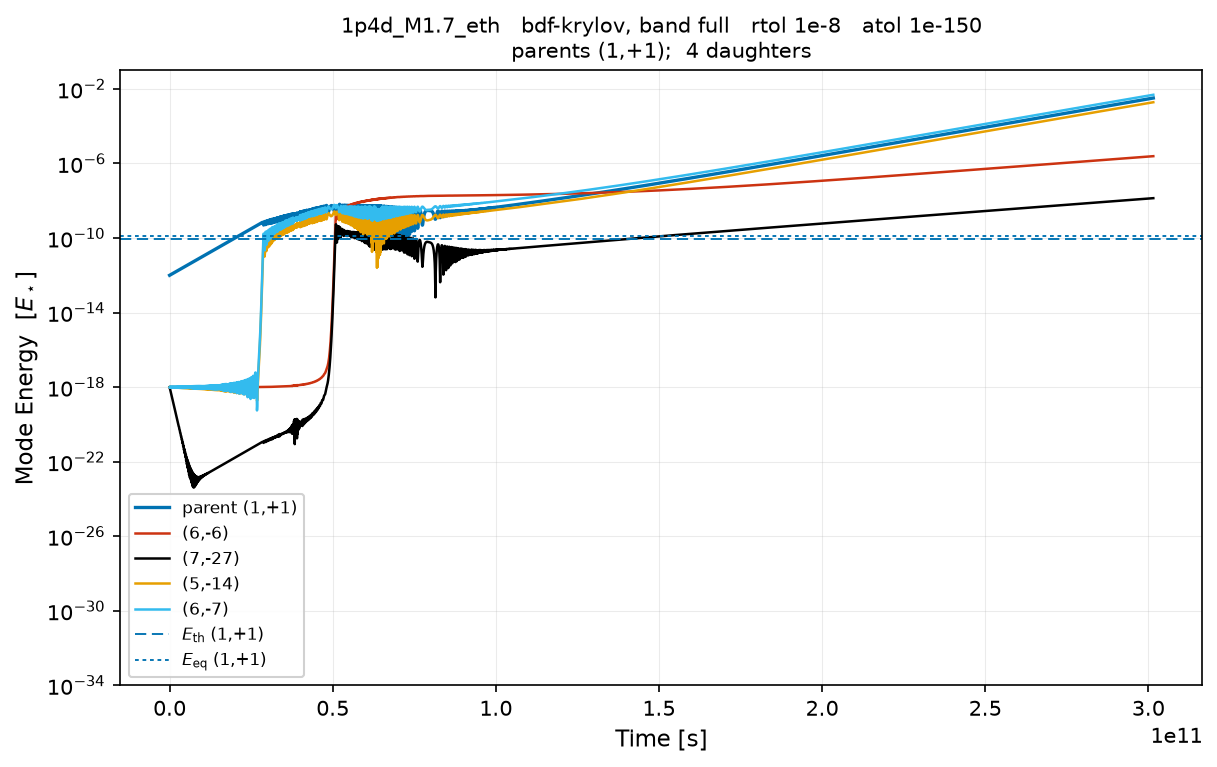
\includegraphics[width=0.21\textwidth,height=0.1323\textwidth]{../plots/krylov_full/1p4d_M1.7_eth/r1e-8_a1e-150.png} & 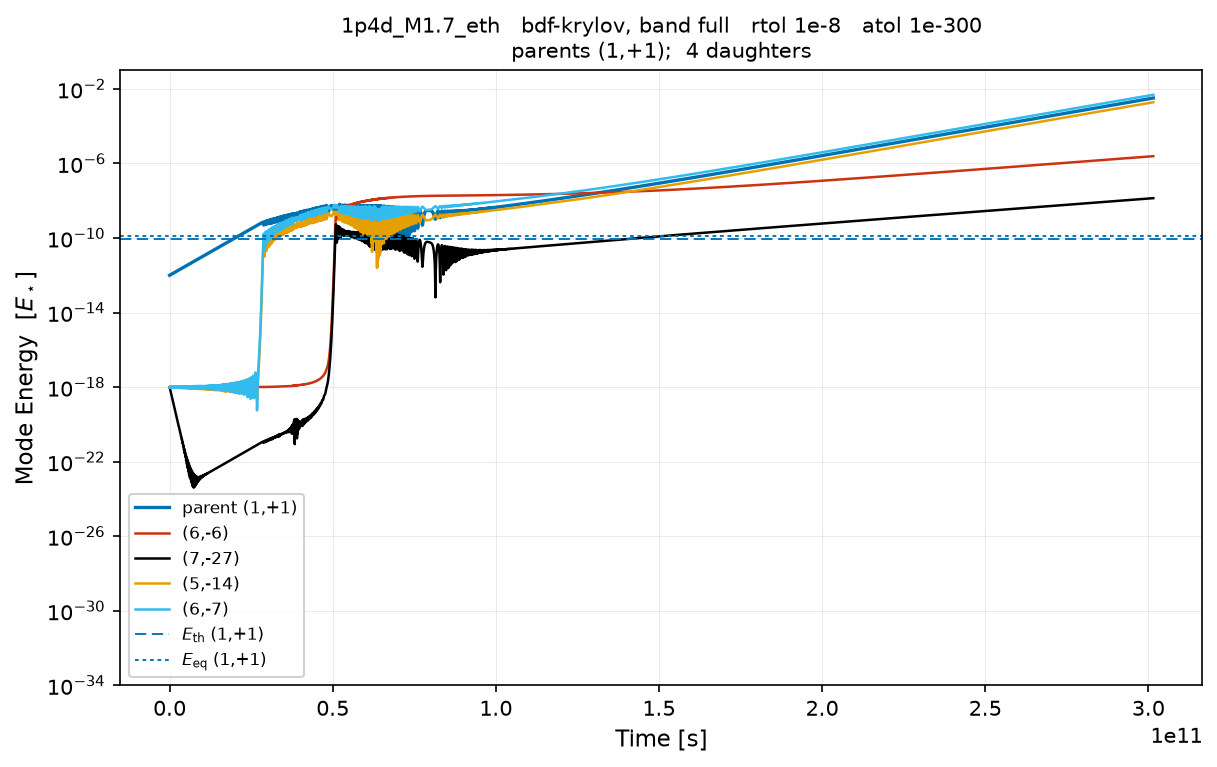
\includegraphics[width=0.21\textwidth,height=0.1323\textwidth]{../plots/krylov_full/1p4d_M1.7_eth/r1e-8_a1e-300.png} & 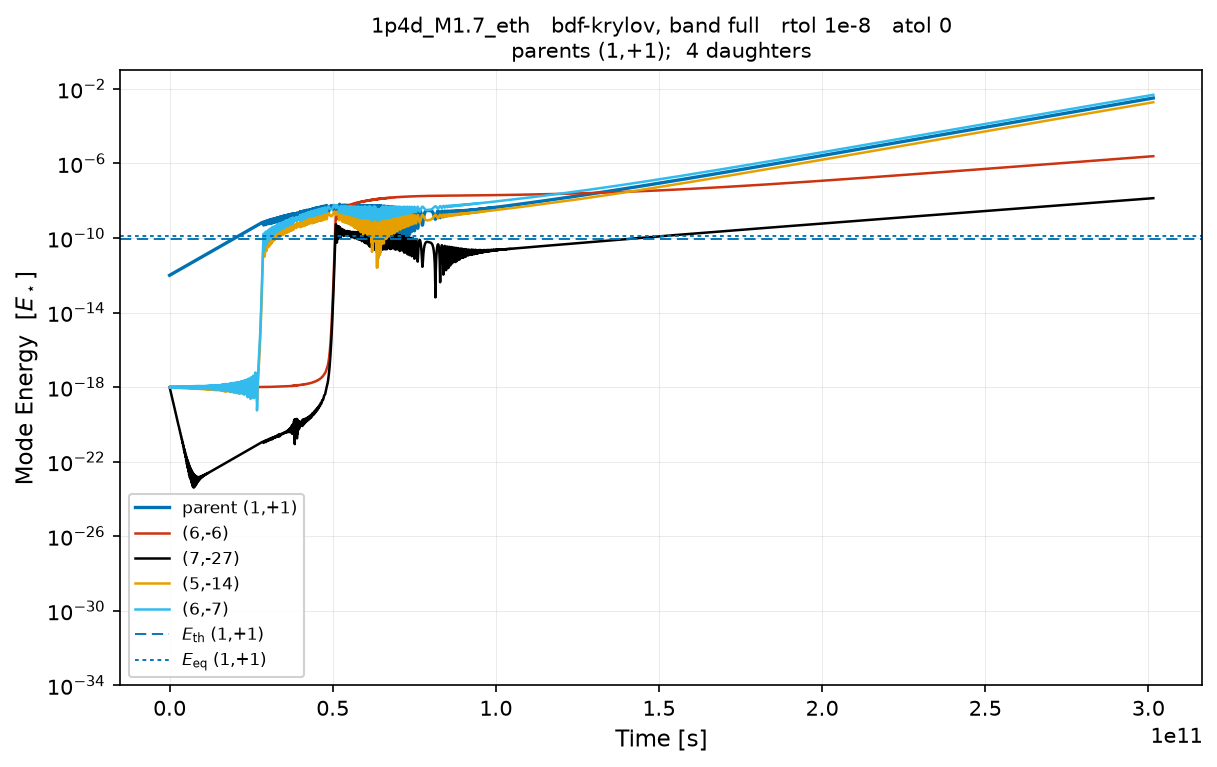
\includegraphics[width=0.21\textwidth,height=0.1323\textwidth]{../plots/krylov_full/1p4d_M1.7_eth/r1e-8_a0.png} \\[-1pt]
 & \parbox[t]{0.21\textwidth}{\centering\scriptsize 69.74\,M steps, 133.2\,s, runaway} & \parbox[t]{0.21\textwidth}{\centering\scriptsize 69.63\,M steps, 134.7\,s, runaway} & \parbox[t]{0.21\textwidth}{\centering\scriptsize 69.63\,M steps, 109.1\,s, runaway} & \parbox[t]{0.21\textwidth}{\centering\scriptsize 69.63\,M steps, 117.5\,s, runaway} \\[2pt]
\rotatebox{90}{\parbox{0.1323\textwidth}{\centering\scriptsize\bfseries BDF-Krylov, band 3}} & 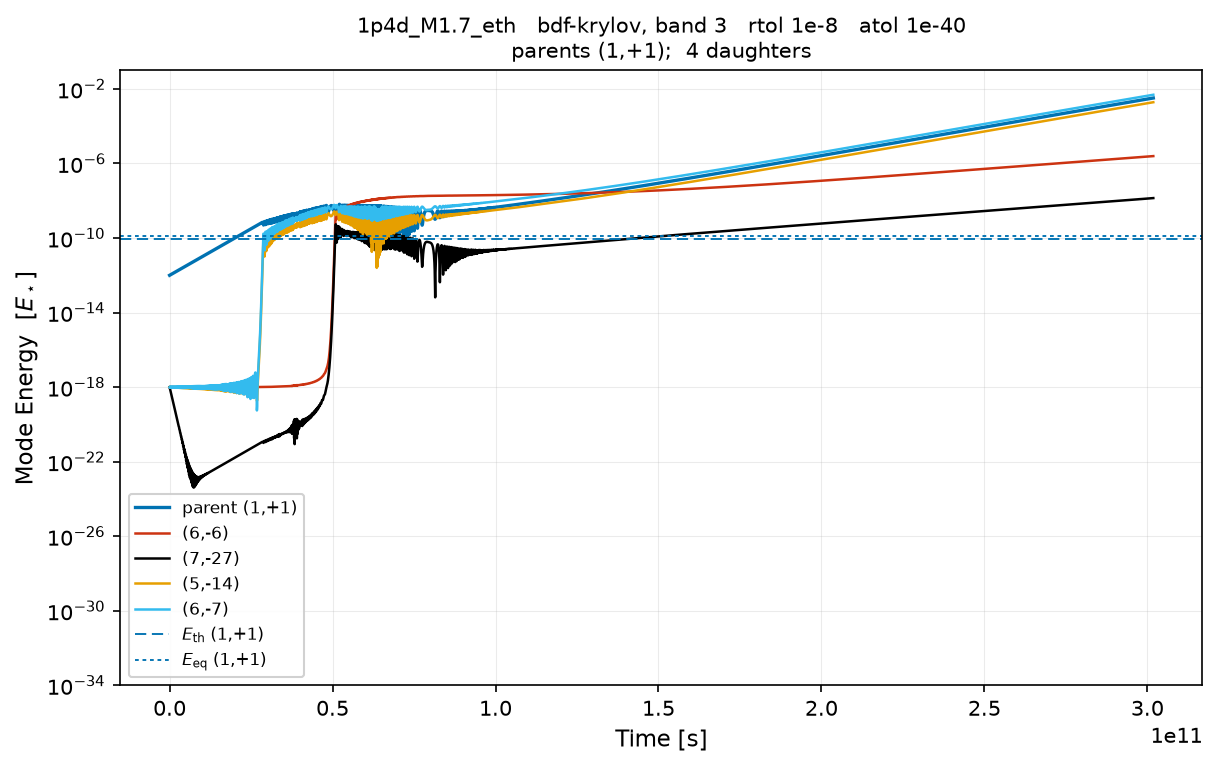
\includegraphics[width=0.21\textwidth,height=0.1323\textwidth]{../plots/krylov_b3/1p4d_M1.7_eth/r1e-8_a1e-40.png} & 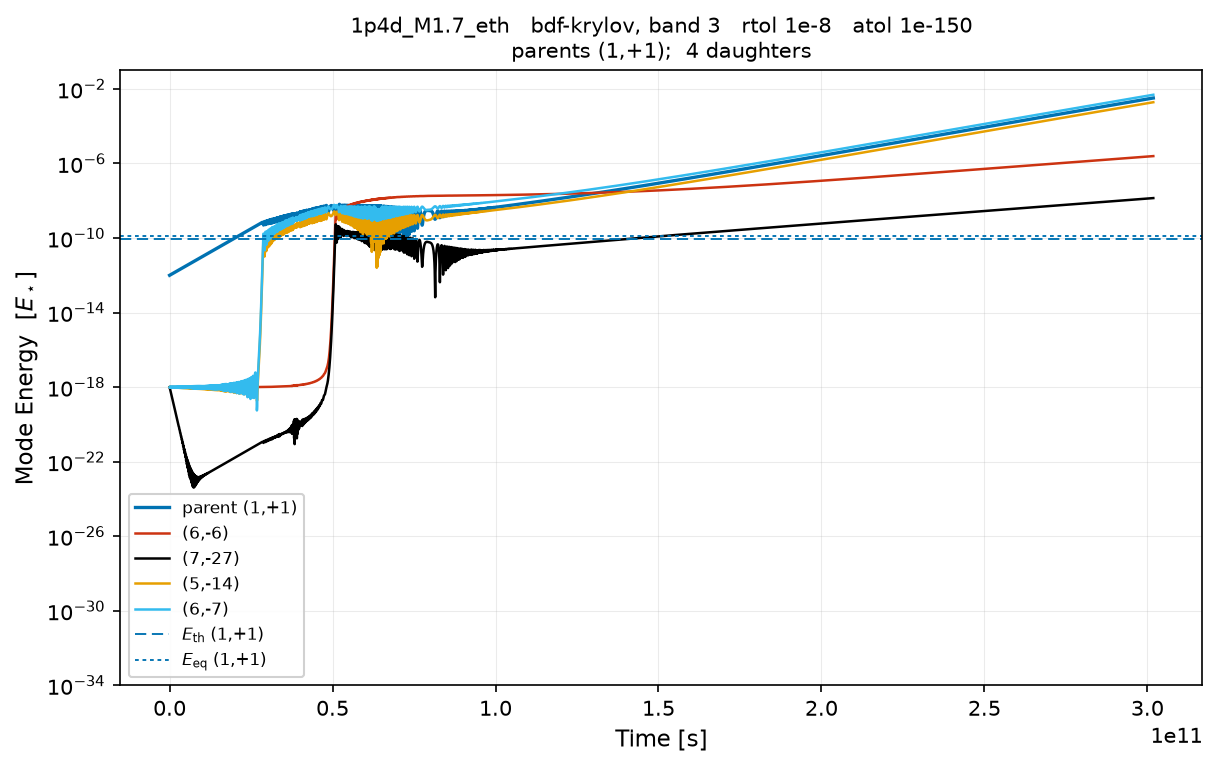
\includegraphics[width=0.21\textwidth,height=0.1323\textwidth]{../plots/krylov_b3/1p4d_M1.7_eth/r1e-8_a1e-150.png} & 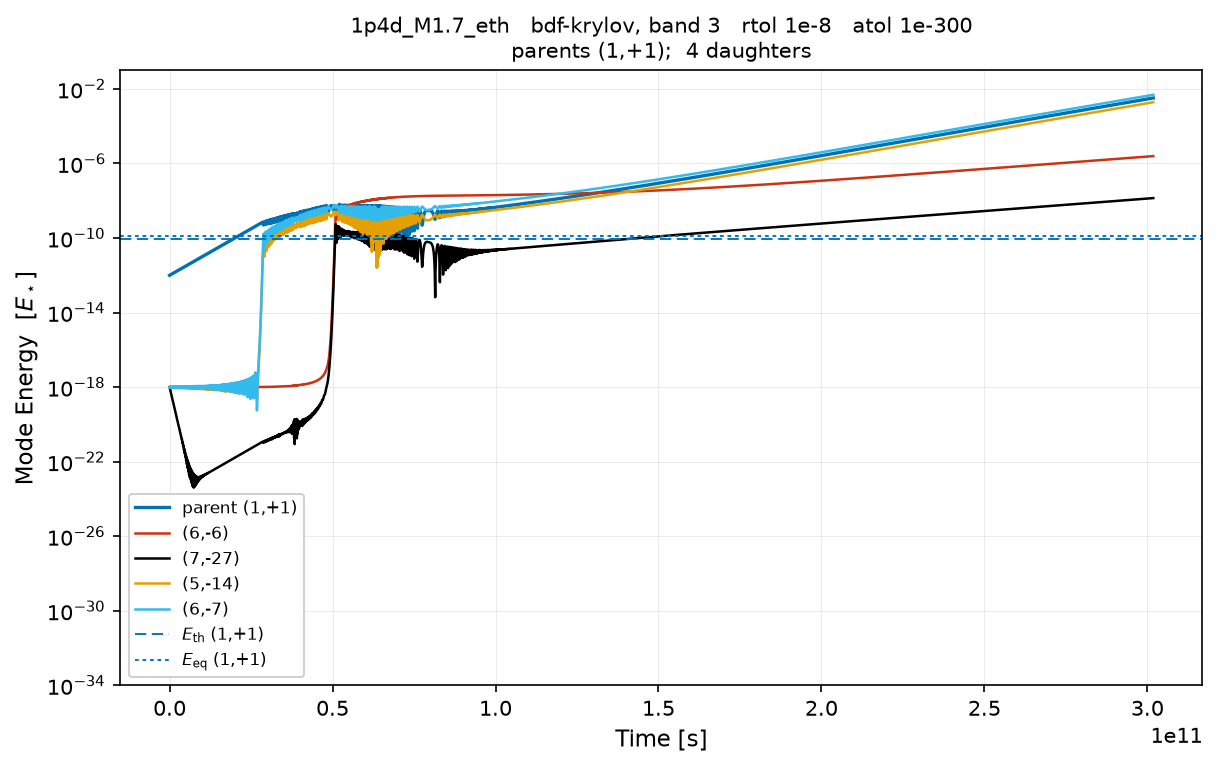
\includegraphics[width=0.21\textwidth,height=0.1323\textwidth]{../plots/krylov_b3/1p4d_M1.7_eth/r1e-8_a1e-300.png} & 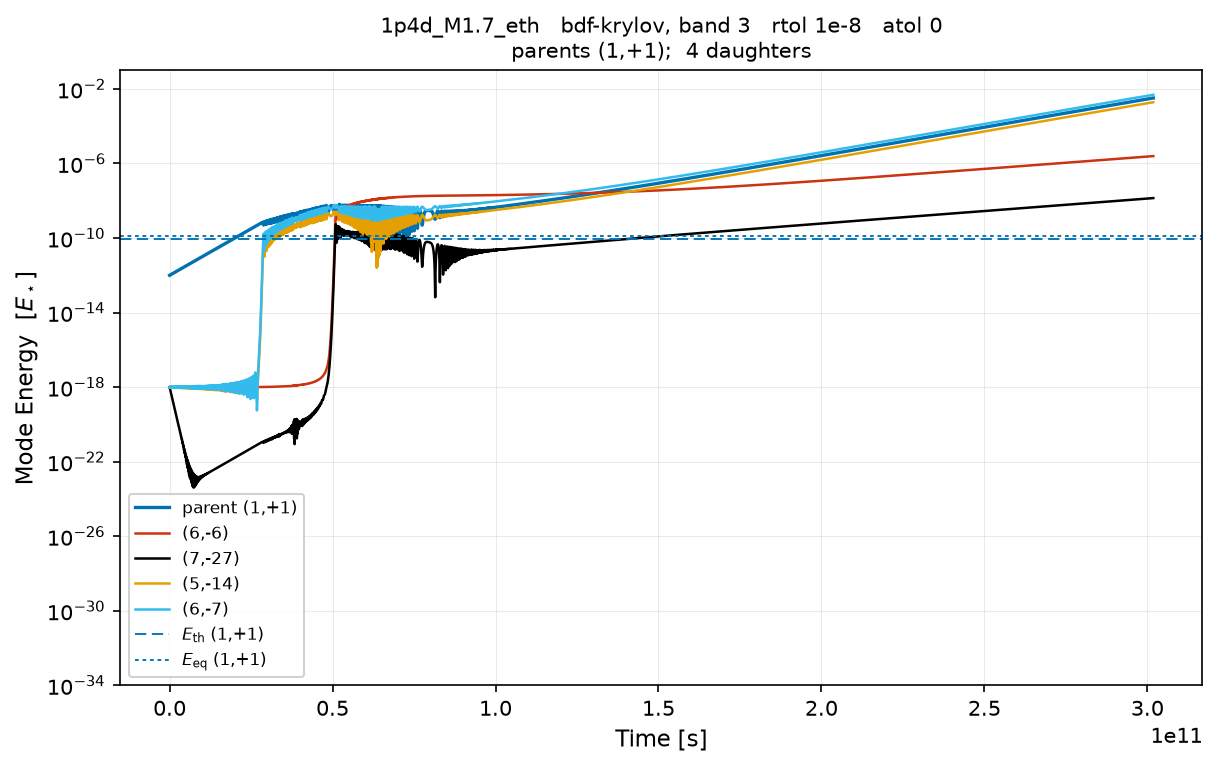
\includegraphics[width=0.21\textwidth,height=0.1323\textwidth]{../plots/krylov_b3/1p4d_M1.7_eth/r1e-8_a0.png} \\[-1pt]
 & \parbox[t]{0.21\textwidth}{\centering\scriptsize 66.98\,M steps, 163.0\,s, runaway} & \parbox[t]{0.21\textwidth}{\centering\scriptsize 66.99\,M steps, 172.6\,s, runaway} & \parbox[t]{0.21\textwidth}{\centering\scriptsize 66.99\,M steps, 176.3\,s, runaway} & \parbox[t]{0.21\textwidth}{\centering\scriptsize 66.99\,M steps, 170.4\,s, runaway} \\[2pt]
\rotatebox{90}{\parbox{0.1323\textwidth}{\centering\scriptsize\bfseries Adams, fixed point}} & 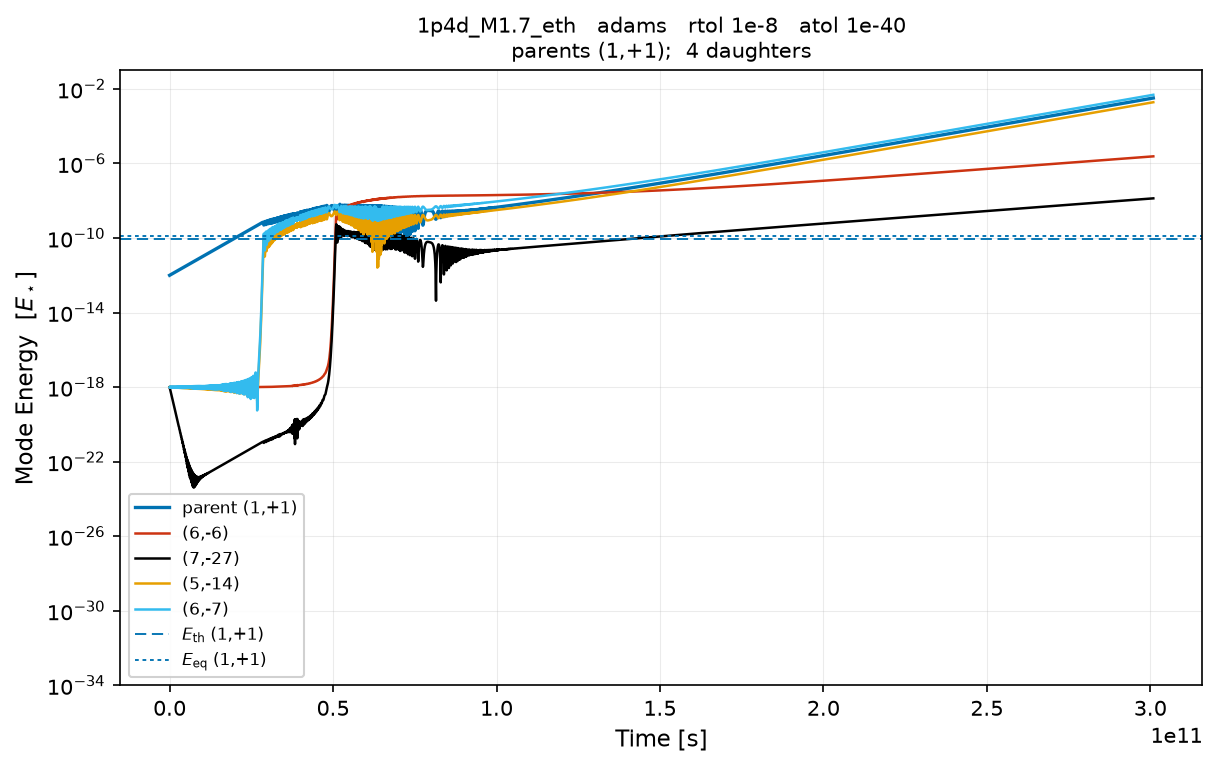
\includegraphics[width=0.21\textwidth,height=0.1323\textwidth]{../plots/adams/1p4d_M1.7_eth/r1e-8_a1e-40.png} & 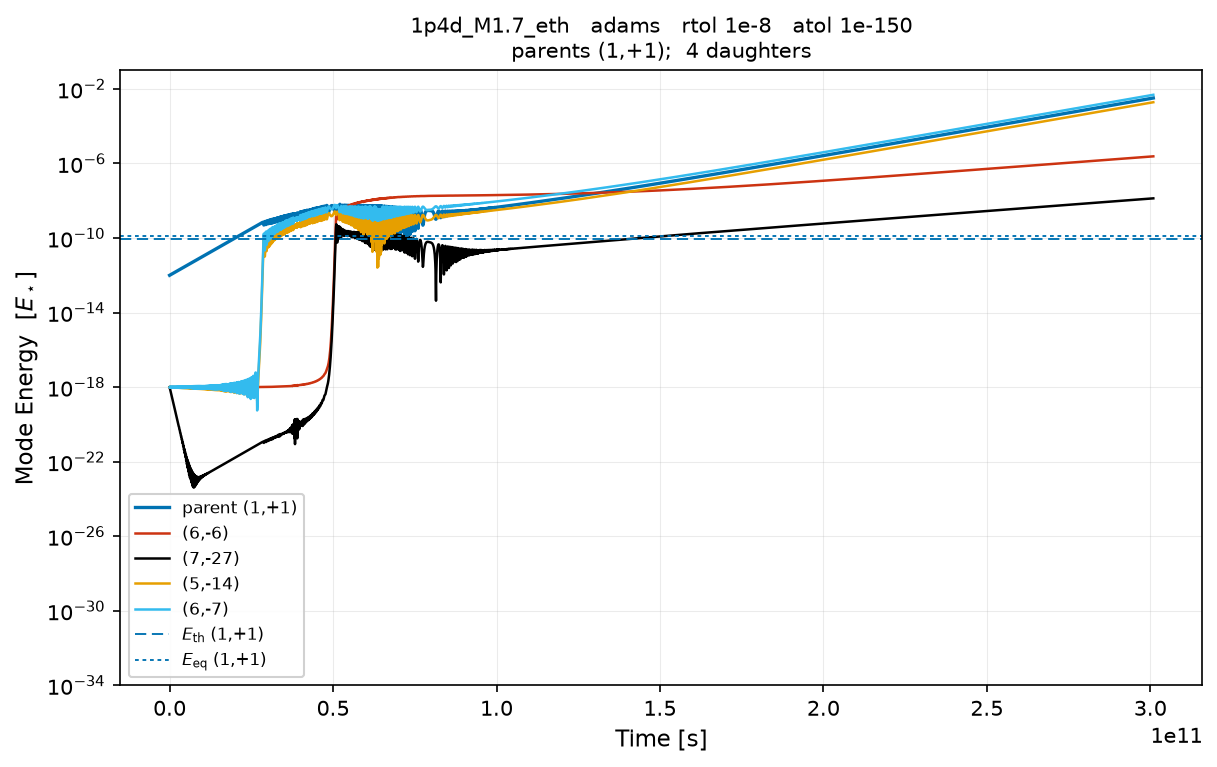
\includegraphics[width=0.21\textwidth,height=0.1323\textwidth]{../plots/adams/1p4d_M1.7_eth/r1e-8_a1e-150.png} & 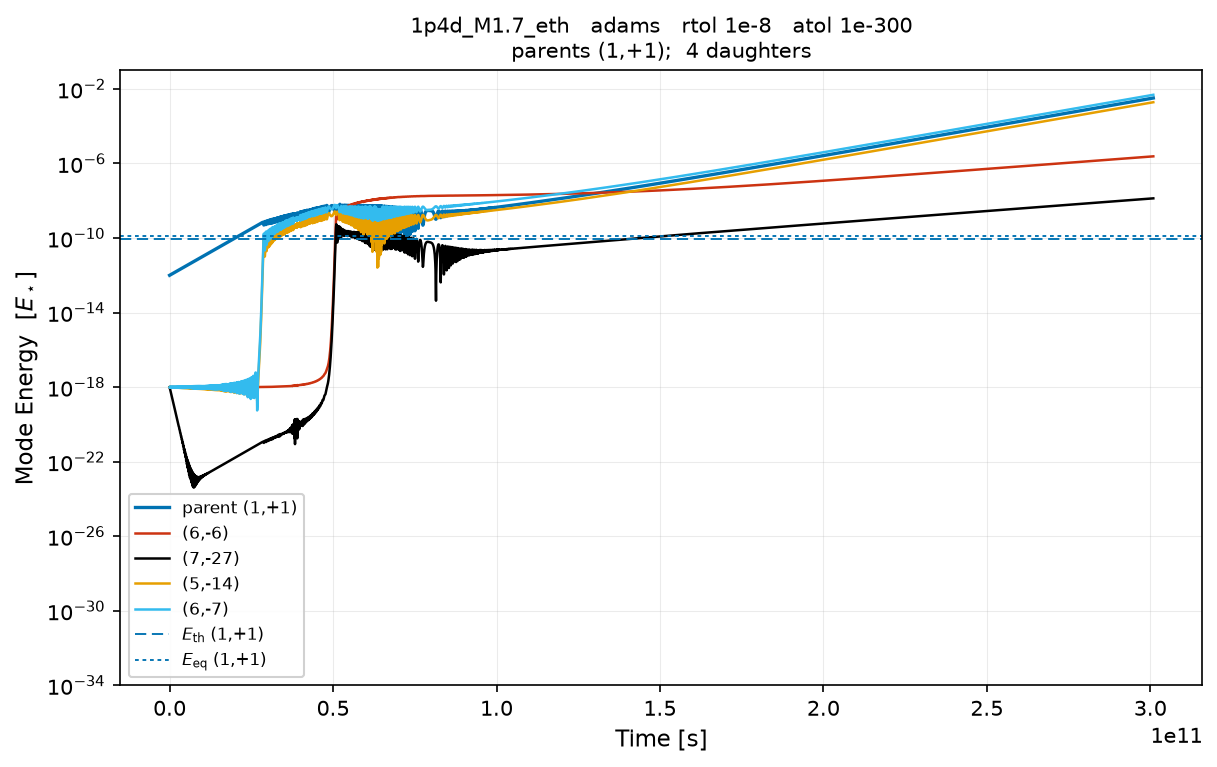
\includegraphics[width=0.21\textwidth,height=0.1323\textwidth]{../plots/adams/1p4d_M1.7_eth/r1e-8_a1e-300.png} & 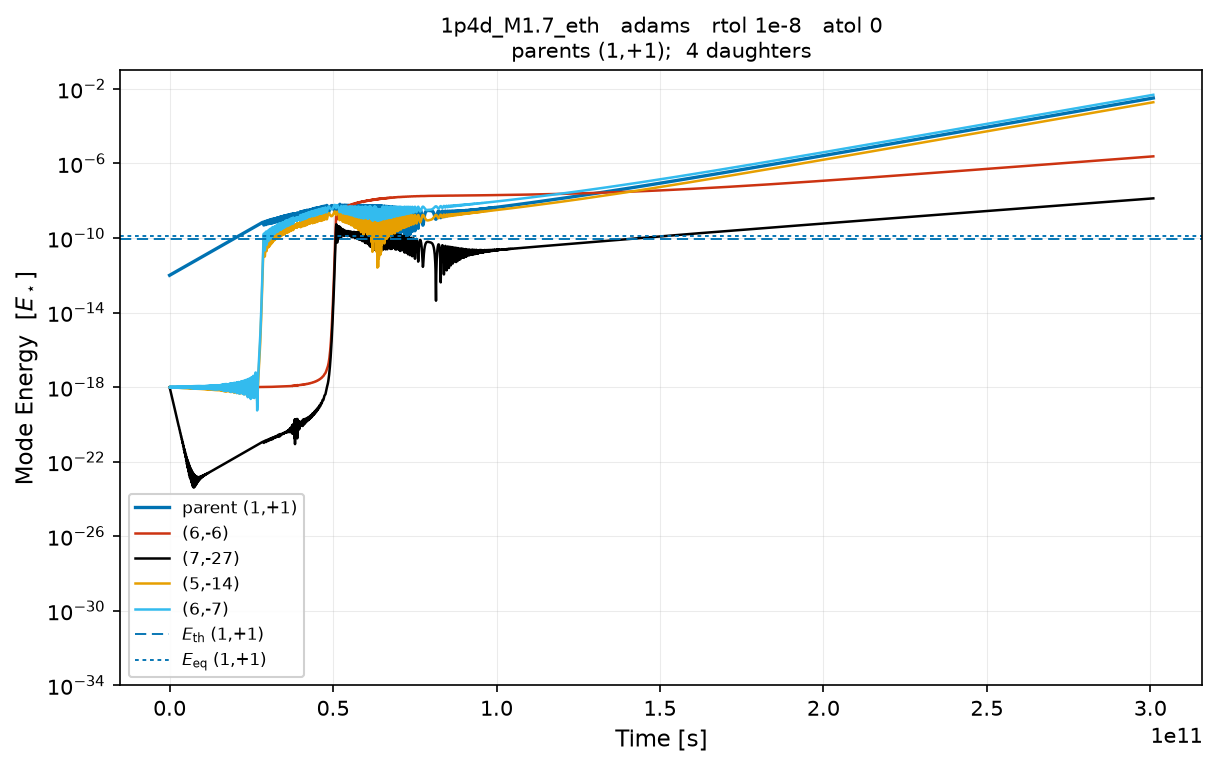
\includegraphics[width=0.21\textwidth,height=0.1323\textwidth]{../plots/adams/1p4d_M1.7_eth/r1e-8_a0.png} \\[-1pt]
 & \parbox[t]{0.21\textwidth}{\centering\scriptsize 42.69\,M steps, 64.2\,s, runaway} & \parbox[t]{0.21\textwidth}{\centering\scriptsize 42.69\,M steps, 50.1\,s, runaway} & \parbox[t]{0.21\textwidth}{\centering\scriptsize 42.69\,M steps, 52.2\,s, runaway} & \parbox[t]{0.21\textwidth}{\centering\scriptsize 42.69\,M steps, 42.8\,s, runaway} \\[2pt]
\end{tabular}\par}
\par\noindent{\scriptsize\setlength\tabcolsep{3.5pt}\renewcommand\arraystretch{0.92}
\begin{tabular}{@{}llllrrrrrrr@{}}
\toprule
integrator & atol & stop & $t_{\rm stop}$ [s] & steps & rejected & RHS & Jac. & NL it. & lin. it. & wall [s] \\
\midrule
rk8pd & $10^{-40}$ & runaway & $3.01\times10^{11}$ & 7.58\,M & 1.01\,M & 98.48\,M & -- & -- & -- & 19.8 \\
 & $10^{-150}$ & runaway & $3.01\times10^{11}$ & 7.58\,M & 1.01\,M & 98.48\,M & -- & -- & -- & 17.7 \\
 & $10^{-300}$ & runaway & $3.01\times10^{11}$ & 7.58\,M & 1.01\,M & 98.48\,M & -- & -- & -- & 18.4 \\
 & $0$ & runaway & $3.01\times10^{11}$ & 7.58\,M & 1.01\,M & 98.48\,M & -- & -- & -- & 19.8 \\
\addlinespace[2pt]
BDF, dense analytic Jacobian & $10^{-40}$ & runaway & $3.01\times10^{11}$ & 72.42\,M & 911.7\,k & 78.90\,M & 1.27\,M & 78.90\,M & -- & 74.9 \\
 & $10^{-150}$ & runaway & $3.01\times10^{11}$ & 72.41\,M & 918.0\,k & 78.93\,M & 1.27\,M & 78.93\,M & -- & 74.4 \\
 & $10^{-300}$ & runaway & $3.01\times10^{11}$ & 72.41\,M & 918.0\,k & 78.93\,M & 1.27\,M & 78.93\,M & -- & 122.1 \\
 & $0$ & runaway & $3.01\times10^{11}$ & 72.41\,M & 918.0\,k & 78.93\,M & 1.27\,M & 78.93\,M & -- & 90.0 \\
\addlinespace[2pt]
BDF-Krylov, band full & $10^{-40}$ & runaway & $3.02\times10^{11}$ & 69.74\,M & 989.6\,k & 163.10\,M & 1.19\,M & 76.22\,M & 75.01\,M & 133.2 \\
 & $10^{-150}$ & runaway & $3.02\times10^{11}$ & 69.63\,M & 1.00\,M & 162.99\,M & 1.19\,M & 76.17\,M & 74.96\,M & 134.7 \\
 & $10^{-300}$ & runaway & $3.02\times10^{11}$ & 69.63\,M & 1.00\,M & 162.99\,M & 1.19\,M & 76.17\,M & 74.96\,M & 109.1 \\
 & $0$ & runaway & $3.02\times10^{11}$ & 69.63\,M & 1.00\,M & 162.99\,M & 1.19\,M & 76.17\,M & 74.96\,M & 117.5 \\
\addlinespace[2pt]
BDF-Krylov, band 3 & $10^{-40}$ & runaway & $3.02\times10^{11}$ & 66.98\,M & 1.31\,M & 186.37\,M & 1.14\,M & 75.07\,M & 103.28\,M & 163.0 \\
 & $10^{-150}$ & runaway & $3.02\times10^{11}$ & 66.99\,M & 1.31\,M & 186.37\,M & 1.14\,M & 75.09\,M & 103.26\,M & 172.6 \\
 & $10^{-300}$ & runaway & $3.02\times10^{11}$ & 66.99\,M & 1.31\,M & 186.37\,M & 1.14\,M & 75.09\,M & 103.26\,M & 176.3 \\
 & $0$ & runaway & $3.02\times10^{11}$ & 66.99\,M & 1.31\,M & 186.37\,M & 1.14\,M & 75.09\,M & 103.26\,M & 170.4 \\
\addlinespace[2pt]
Adams, fixed point & $10^{-40}$ & runaway & $3.01\times10^{11}$ & 42.69\,M & 2.54\,M & 68.34\,M & -- & 68.34\,M & -- & 64.2 \\
 & $10^{-150}$ & runaway & $3.01\times10^{11}$ & 42.69\,M & 2.54\,M & 68.34\,M & -- & 68.34\,M & -- & 50.1 \\
 & $10^{-300}$ & runaway & $3.01\times10^{11}$ & 42.69\,M & 2.54\,M & 68.34\,M & -- & 68.34\,M & -- & 52.2 \\
 & $0$ & runaway & $3.01\times10^{11}$ & 42.69\,M & 2.54\,M & 68.34\,M & -- & 68.34\,M & -- & 42.8 \\
\bottomrule
\end{tabular}}

\clearpage
\subsection{\texttt{1p4d\_M2.0T\_eth}}\label{net:1p4d_M2.0T_eth}
\noindent\begin{minipage}[t]{0.43\textwidth}\vspace{0pt}\footnotesize
\begin{tabular}{@{}rrlrr@{}}
\toprule
id & gen & $(\ell,n)$ & $\omega$ [rad\,s$^{-1}$] & $\gamma$ [s$^{-1}$] \\
\midrule
0 & 0 & (2,$-$2) & $7.959\times10^{-4}$ & $-6.697\times10^{-11}$ \\
1 & 1 & (3,$-$31) & $1.287\times10^{-4}$ & $8.096\times10^{-11}$ \\
2 & 1 & (5,$-$8) & $6.672\times10^{-4}$ & $7.367\times10^{-13}$ \\
3 & 1 & (5,$-$9) & $6.216\times10^{-4}$ & $1.110\times10^{-12}$ \\
4 & 1 & (7,$-$50) & $1.743\times10^{-4}$ & $2.546\times10^{-9}$ \\
\bottomrule
\end{tabular}
\end{minipage}\hfill
\begin{minipage}[t]{0.55\textwidth}\vspace{0pt}\footnotesize
\textbf{Model} \texttt{dsct\_M2.0\_T7696}, rule eth, $N=4$, cut 0.15,
closure 0.005; 5 modes, 2 triplet(s).\\[2pt]
\textbf{Selecting pairs}\\ (2,$-$2) $\to$ (3,$-$31) + (5,$-$8): $\Delta/\omega_a=-3.69\times10^{-6}$, $\kappa=+0.215$, $E_{\rm th}=4.87\times10^{-12}$, $E_{\rm eq}=1.50\times10^{-10}$\\
(2,$-$2) $\to$ (5,$-$9) + (7,$-$50): $\Delta/\omega_a=7.51\times10^{-5}$, $\kappa=+0.053$, $E_{\rm th}=1.30\times10^{-9}$, $E_{\rm eq}=1.37\times10^{-9}$\\[2pt]

\end{minipage}

\par\smallskip{\centering\begin{tabular}{@{}c@{\hspace{2pt}}c@{\hspace{2pt}}c@{\hspace{2pt}}c@{\hspace{2pt}}c@{}}
 & \small atol $10^{-40}$ & \small atol $10^{-150}$ & \small atol $10^{-300}$ & \small atol $0$ \\[1pt]
\rotatebox{90}{\parbox{0.1323\textwidth}{\centering\scriptsize\bfseries rk8pd}} & 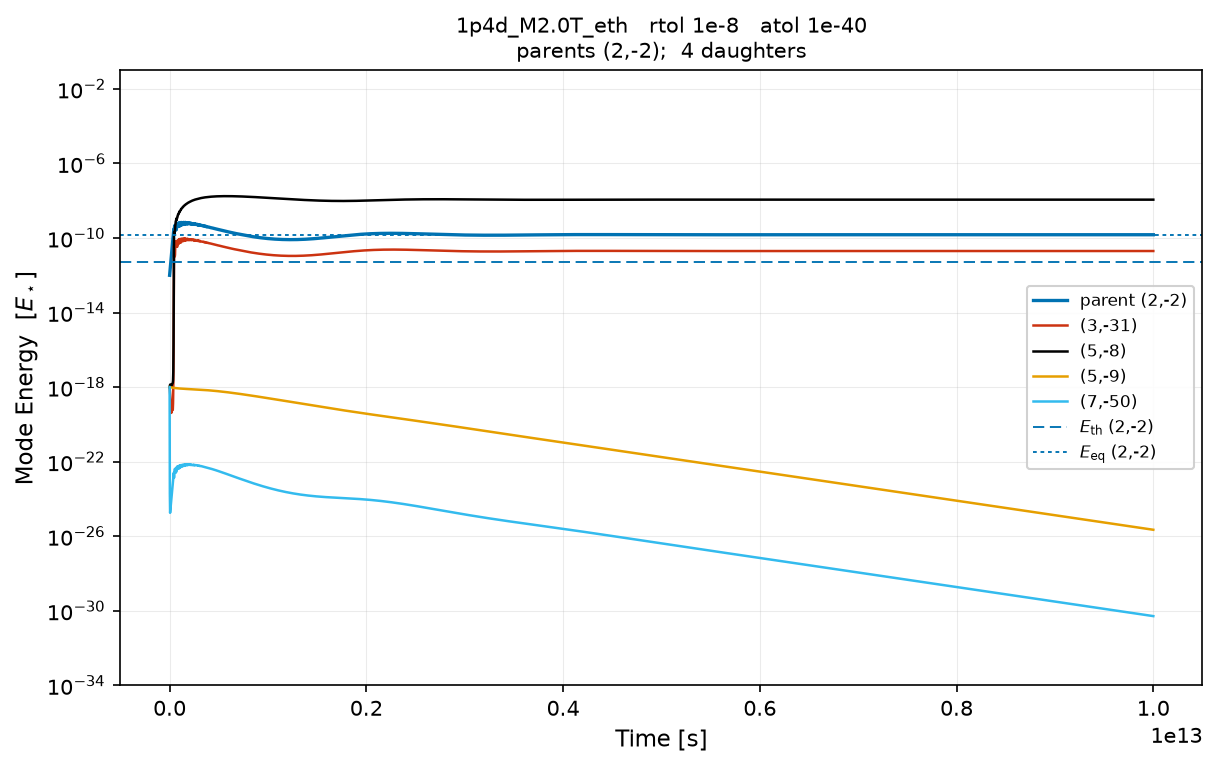
\includegraphics[width=0.21\textwidth,height=0.1323\textwidth]{../plots/rk8pd/1p4d_M2.0T_eth/r1e-8_a1e-40.png} & 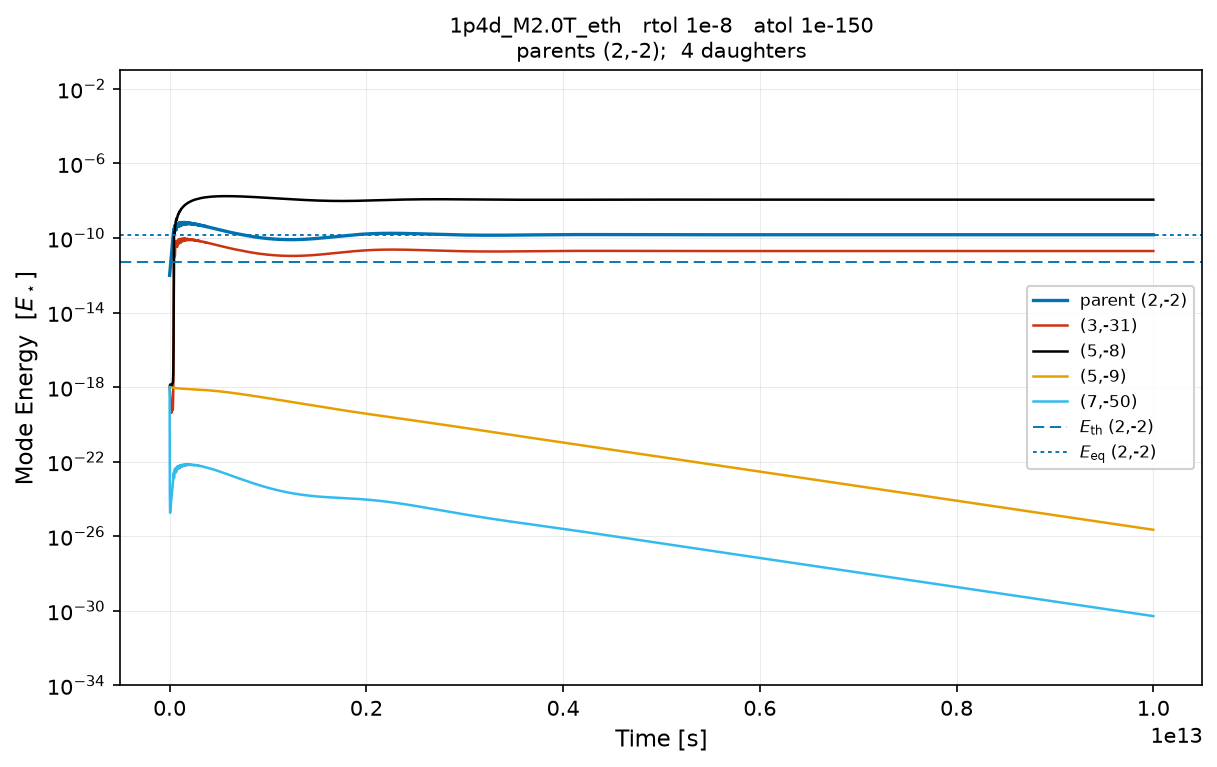
\includegraphics[width=0.21\textwidth,height=0.1323\textwidth]{../plots/rk8pd/1p4d_M2.0T_eth/r1e-8_a1e-150.png} & 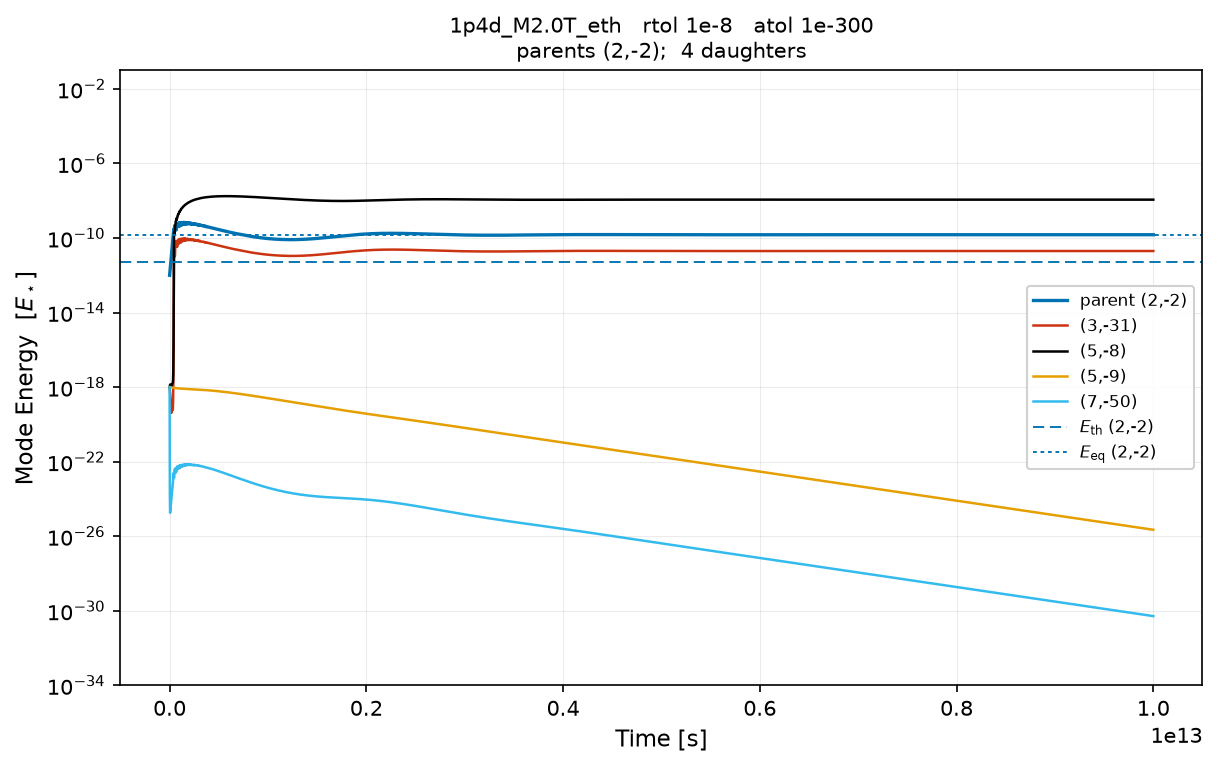
\includegraphics[width=0.21\textwidth,height=0.1323\textwidth]{../plots/rk8pd/1p4d_M2.0T_eth/r1e-8_a1e-300.png} & 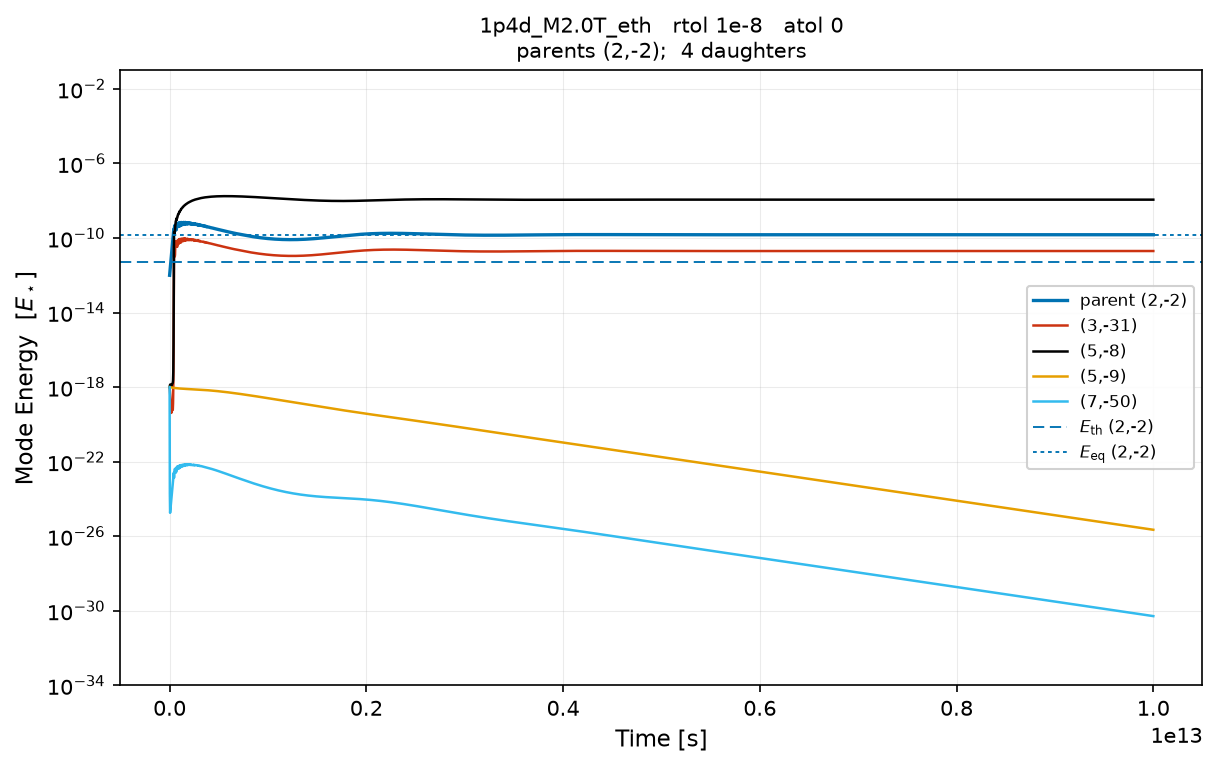
\includegraphics[width=0.21\textwidth,height=0.1323\textwidth]{../plots/rk8pd/1p4d_M2.0T_eth/r1e-8_a0.png} \\[-1pt]
 & \parbox[t]{0.21\textwidth}{\centering\scriptsize 618.4\,k steps, 1.8\,s} & \parbox[t]{0.21\textwidth}{\centering\scriptsize 618.5\,k steps, 2.5\,s} & \parbox[t]{0.21\textwidth}{\centering\scriptsize 618.5\,k steps, 1.2\,s} & \parbox[t]{0.21\textwidth}{\centering\scriptsize 618.5\,k steps, 2.7\,s} \\[2pt]
\rotatebox{90}{\parbox{0.1323\textwidth}{\centering\scriptsize\bfseries BDF, dense analytic Jacobian}} & 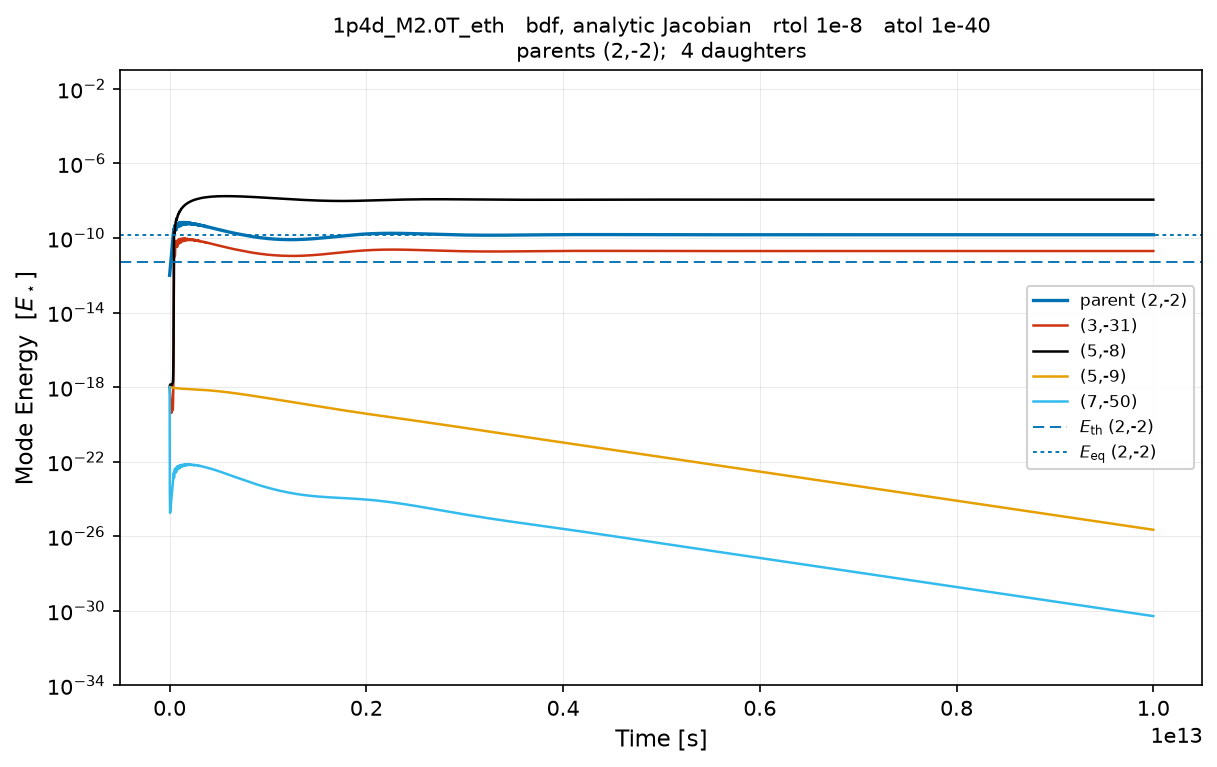
\includegraphics[width=0.21\textwidth,height=0.1323\textwidth]{../plots/bdf/1p4d_M2.0T_eth/r1e-8_a1e-40.png} & 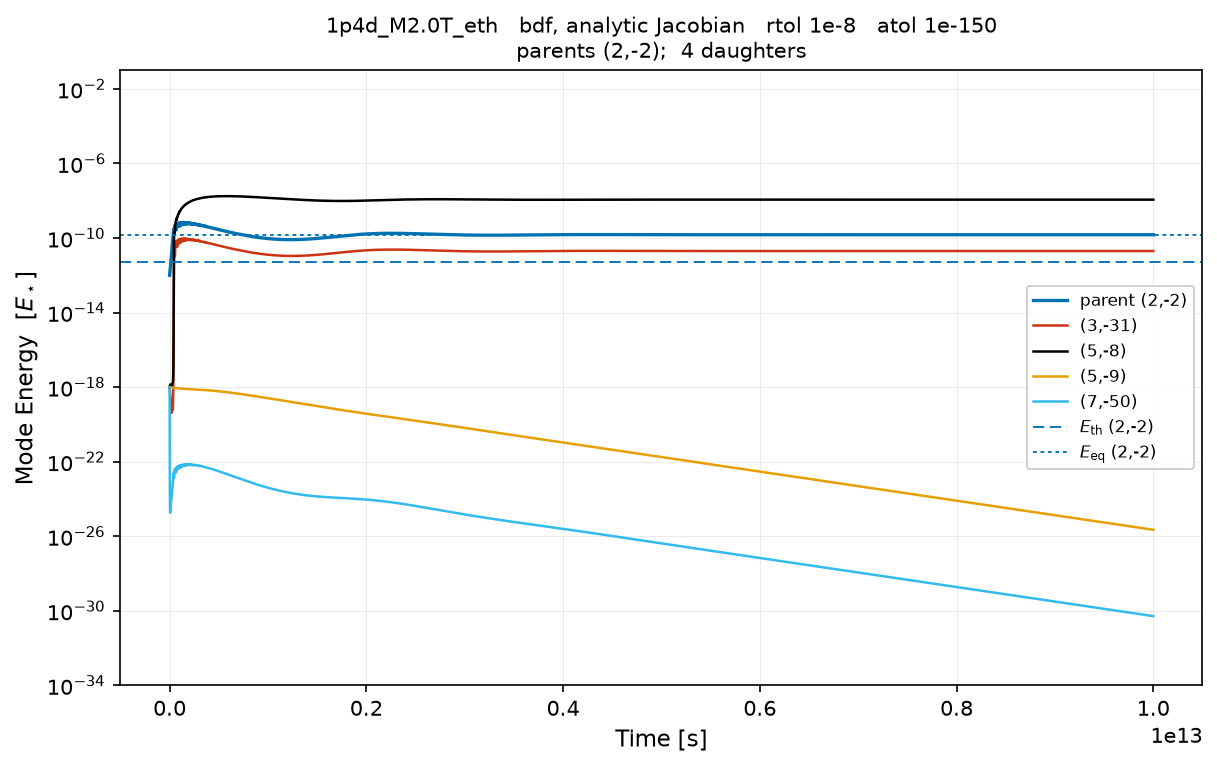
\includegraphics[width=0.21\textwidth,height=0.1323\textwidth]{../plots/bdf/1p4d_M2.0T_eth/r1e-8_a1e-150.png} & 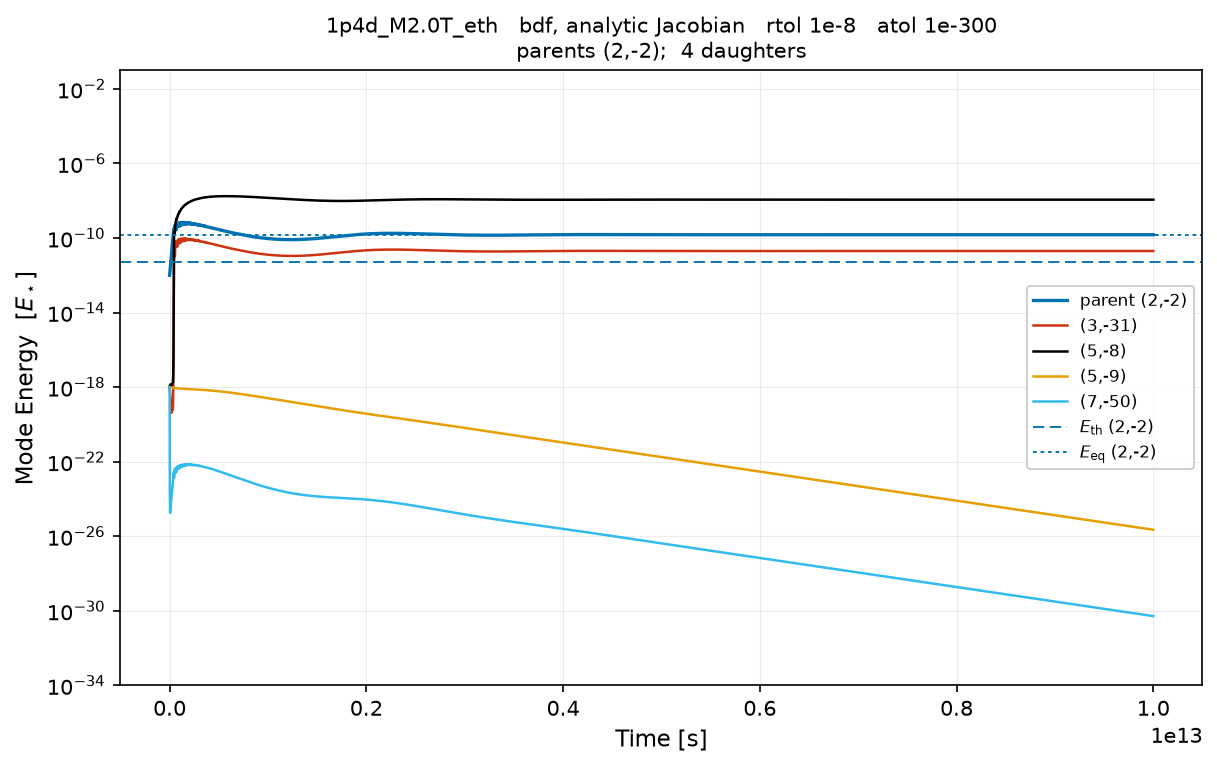
\includegraphics[width=0.21\textwidth,height=0.1323\textwidth]{../plots/bdf/1p4d_M2.0T_eth/r1e-8_a1e-300.png} & 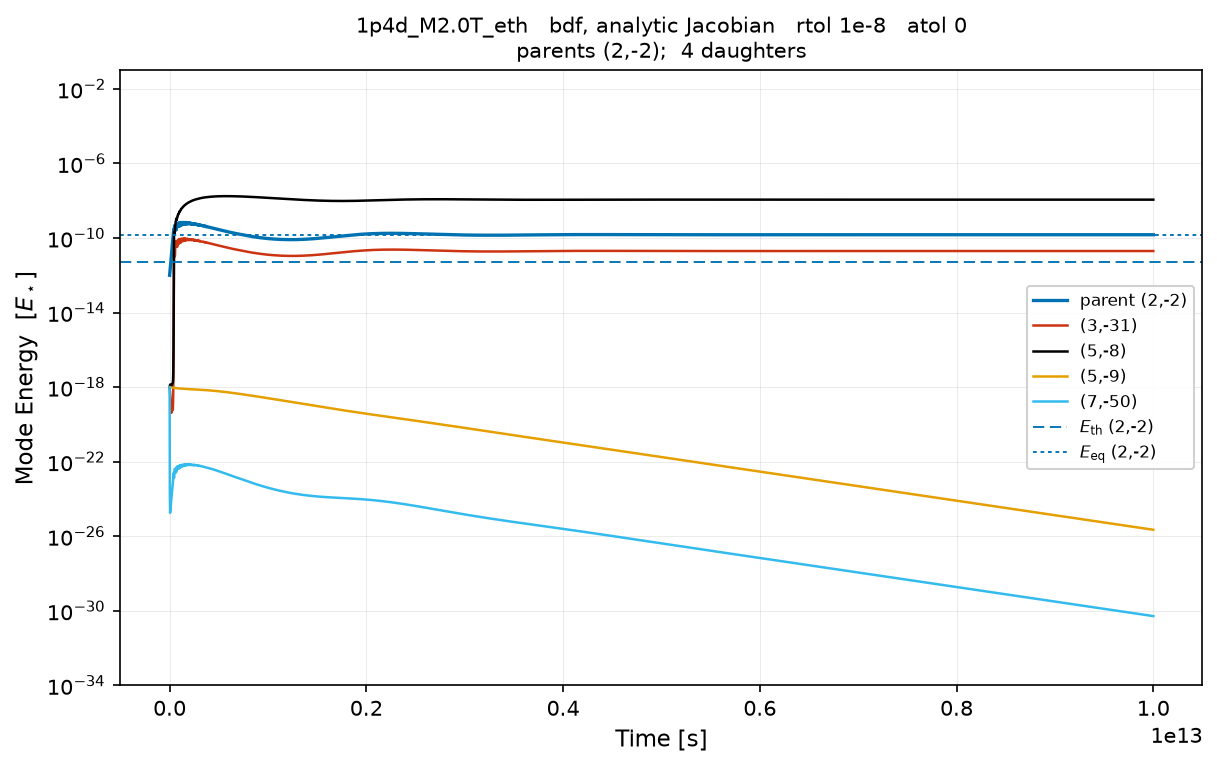
\includegraphics[width=0.21\textwidth,height=0.1323\textwidth]{../plots/bdf/1p4d_M2.0T_eth/r1e-8_a0.png} \\[-1pt]
 & \parbox[t]{0.21\textwidth}{\centering\scriptsize 9.43\,M steps, 8.3\,s} & \parbox[t]{0.21\textwidth}{\centering\scriptsize 9.42\,M steps, 9.5\,s} & \parbox[t]{0.21\textwidth}{\centering\scriptsize 9.42\,M steps, 9.7\,s} & \parbox[t]{0.21\textwidth}{\centering\scriptsize 9.42\,M steps, 11.1\,s} \\[2pt]
\rotatebox{90}{\parbox{0.1323\textwidth}{\centering\scriptsize\bfseries BDF-Krylov, band full}} & 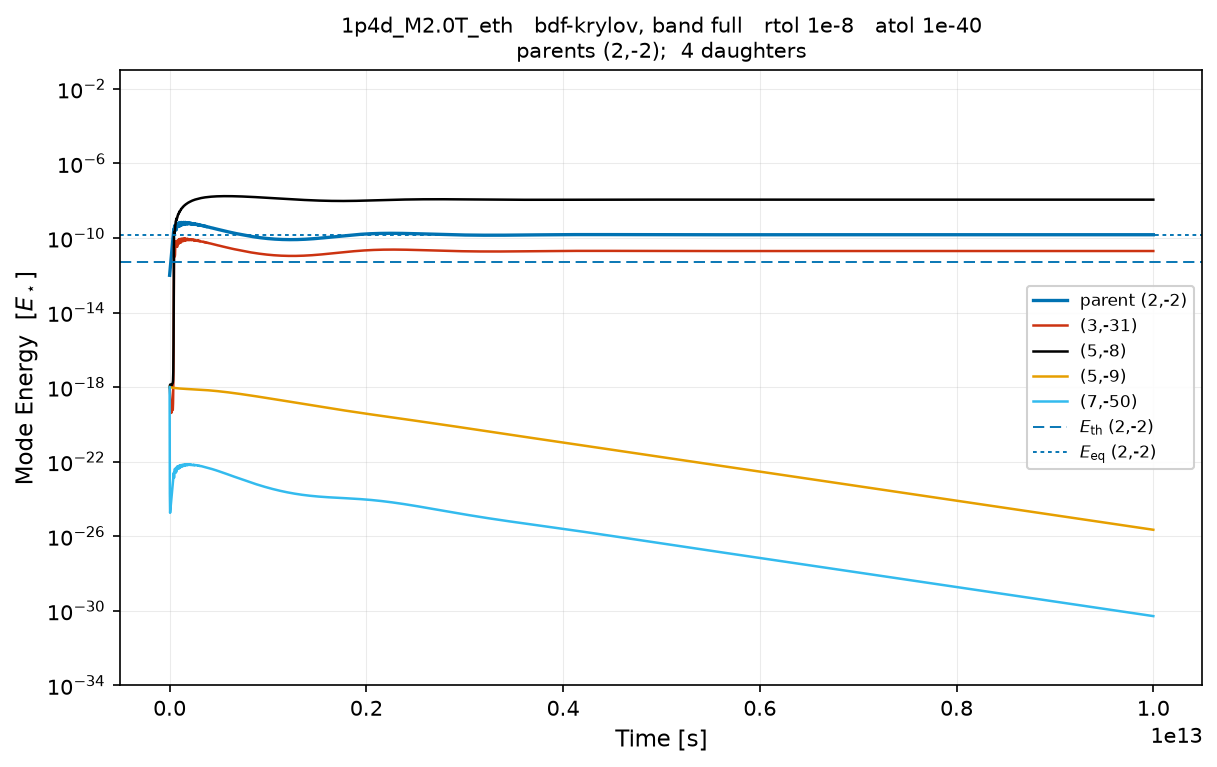
\includegraphics[width=0.21\textwidth,height=0.1323\textwidth]{../plots/krylov_full/1p4d_M2.0T_eth/r1e-8_a1e-40.png} & 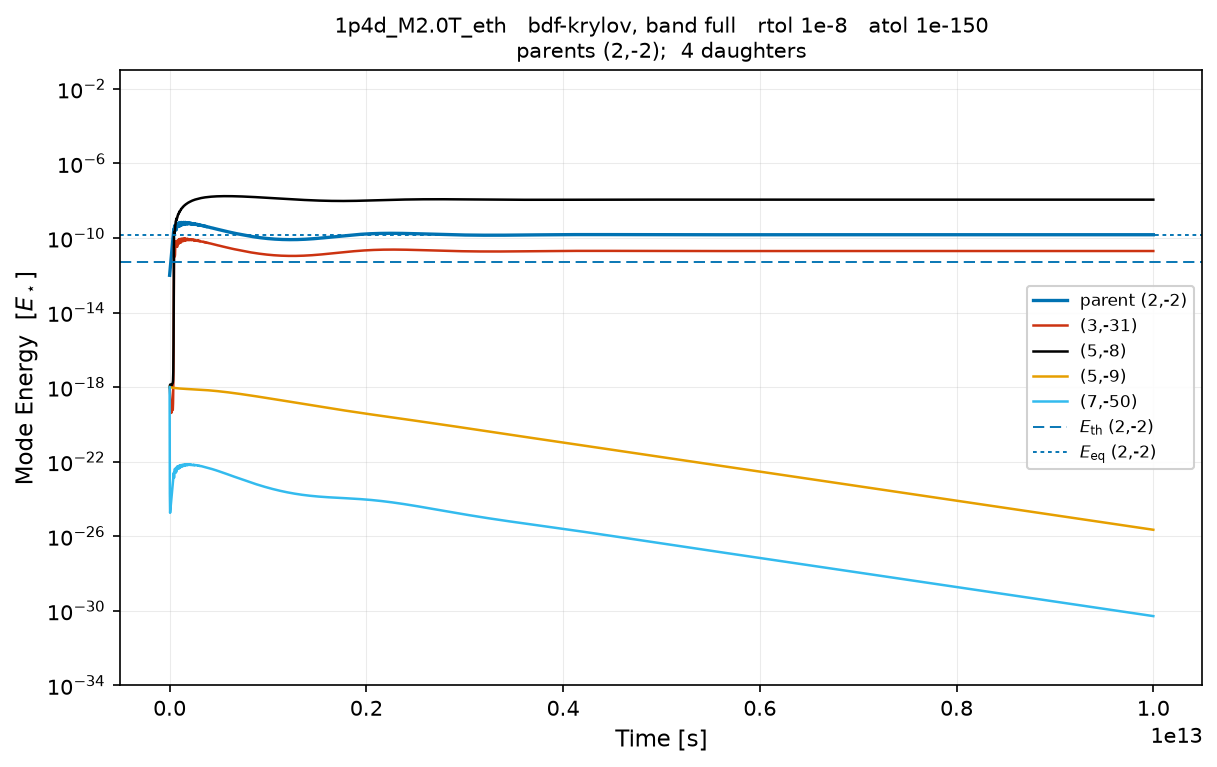
\includegraphics[width=0.21\textwidth,height=0.1323\textwidth]{../plots/krylov_full/1p4d_M2.0T_eth/r1e-8_a1e-150.png} & 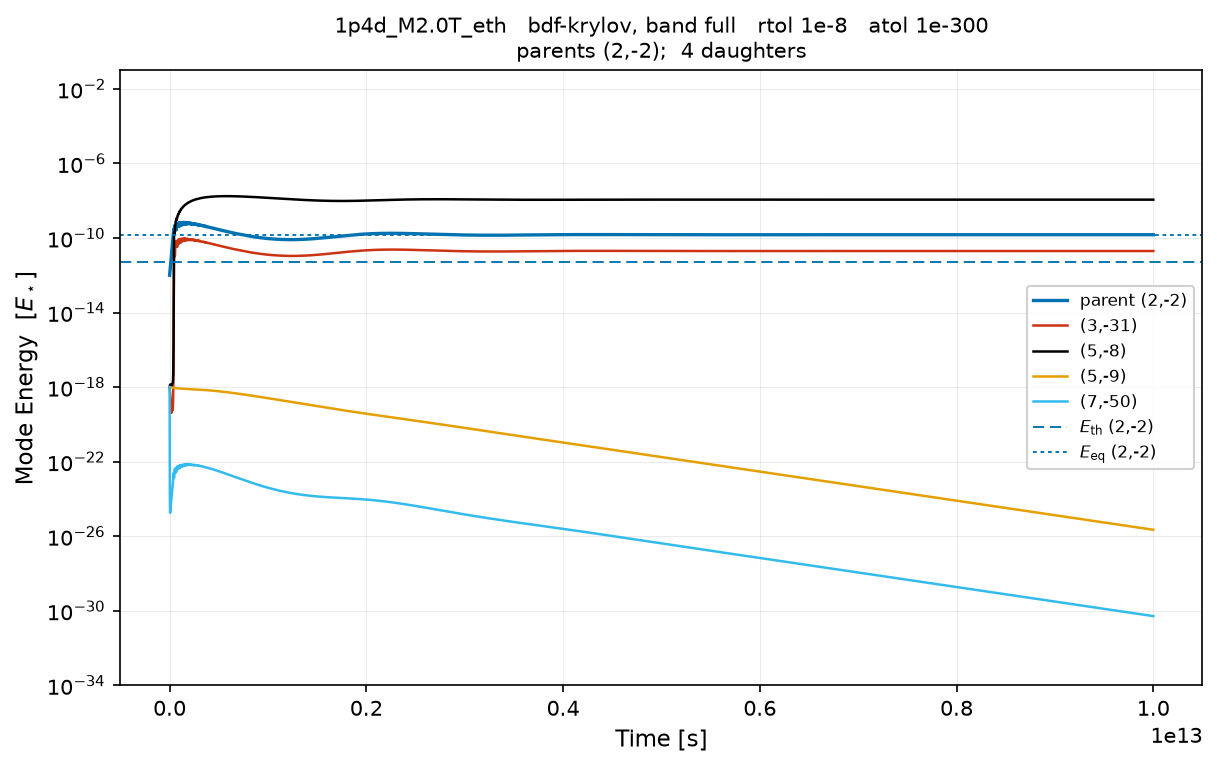
\includegraphics[width=0.21\textwidth,height=0.1323\textwidth]{../plots/krylov_full/1p4d_M2.0T_eth/r1e-8_a1e-300.png} & 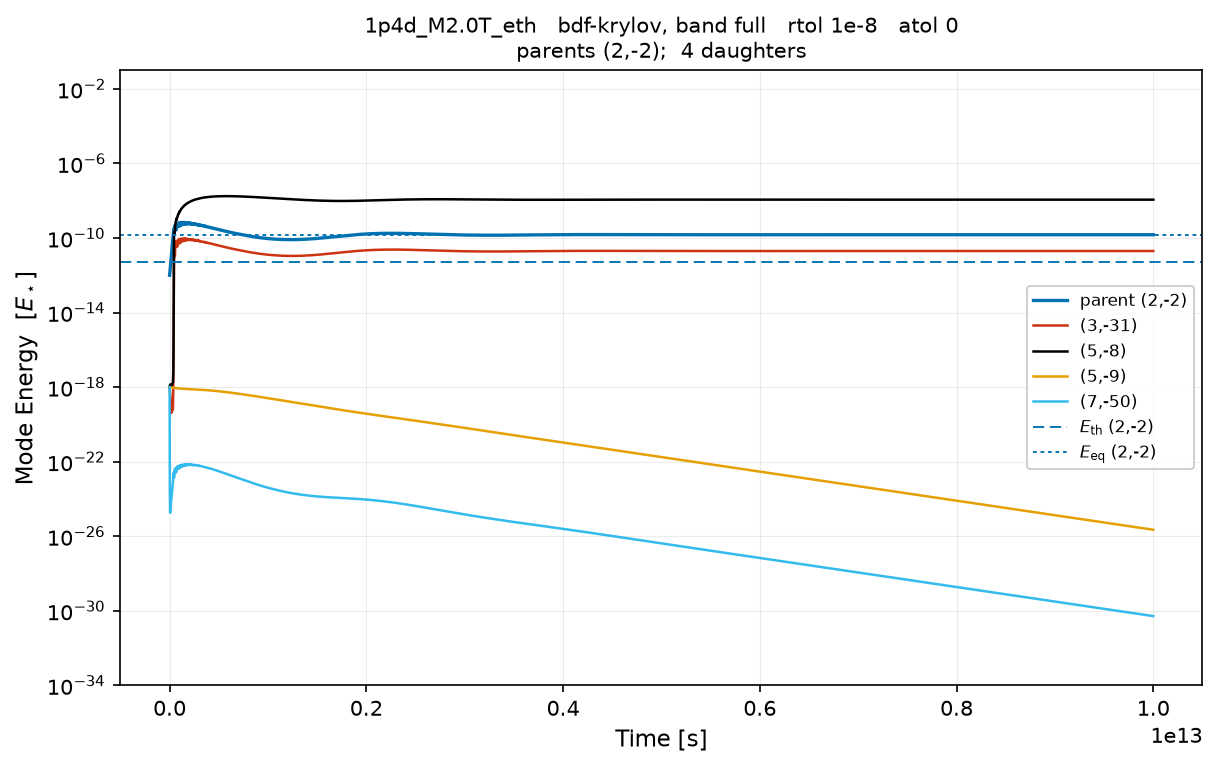
\includegraphics[width=0.21\textwidth,height=0.1323\textwidth]{../plots/krylov_full/1p4d_M2.0T_eth/r1e-8_a0.png} \\[-1pt]
 & \parbox[t]{0.21\textwidth}{\centering\scriptsize 9.43\,M steps, 23.2\,s} & \parbox[t]{0.21\textwidth}{\centering\scriptsize 9.43\,M steps, 23.7\,s} & \parbox[t]{0.21\textwidth}{\centering\scriptsize 9.43\,M steps, 13.0\,s} & \parbox[t]{0.21\textwidth}{\centering\scriptsize 9.43\,M steps, 14.4\,s} \\[2pt]
\rotatebox{90}{\parbox{0.1323\textwidth}{\centering\scriptsize\bfseries BDF-Krylov, band 3}} & 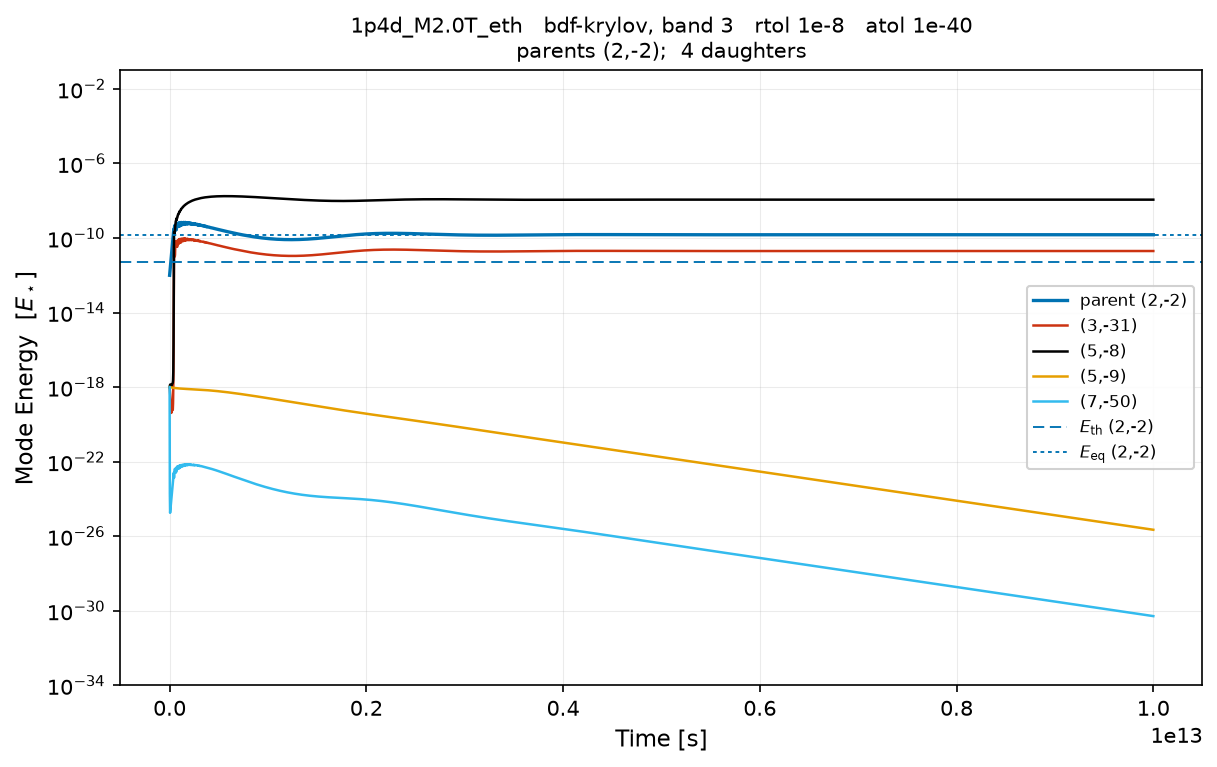
\includegraphics[width=0.21\textwidth,height=0.1323\textwidth]{../plots/krylov_b3/1p4d_M2.0T_eth/r1e-8_a1e-40.png} & 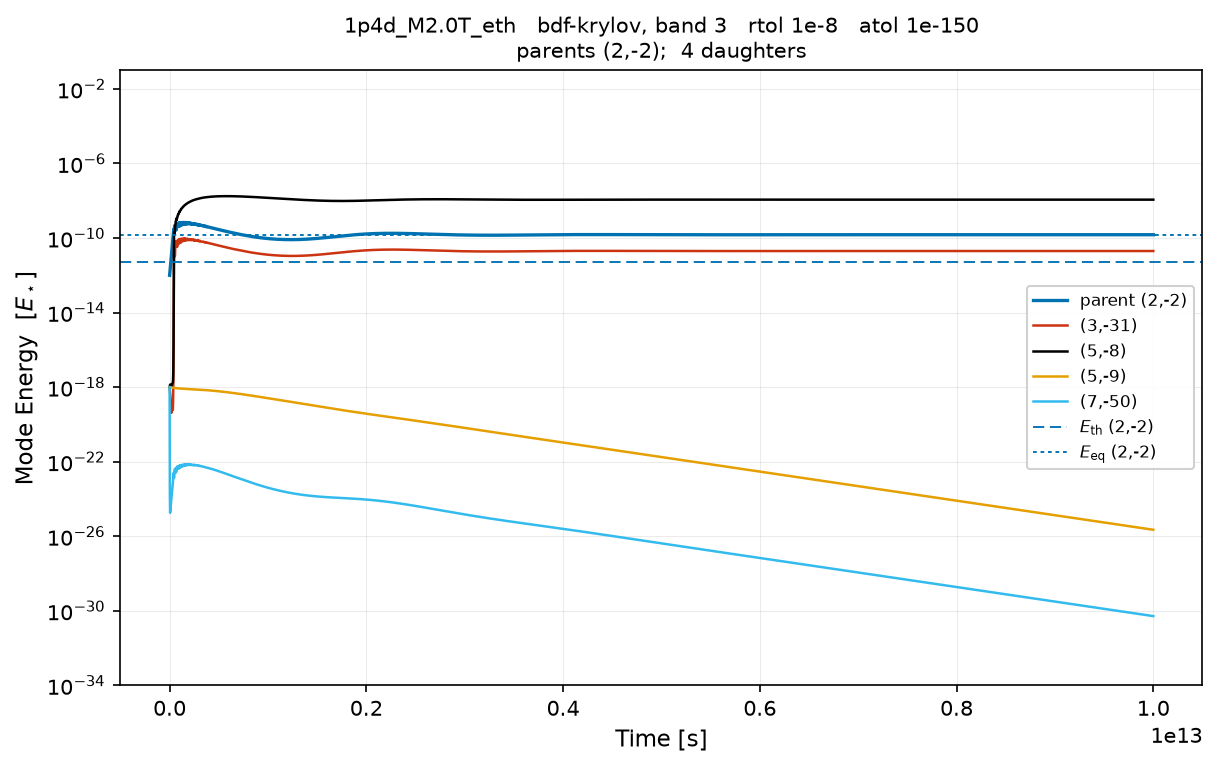
\includegraphics[width=0.21\textwidth,height=0.1323\textwidth]{../plots/krylov_b3/1p4d_M2.0T_eth/r1e-8_a1e-150.png} & 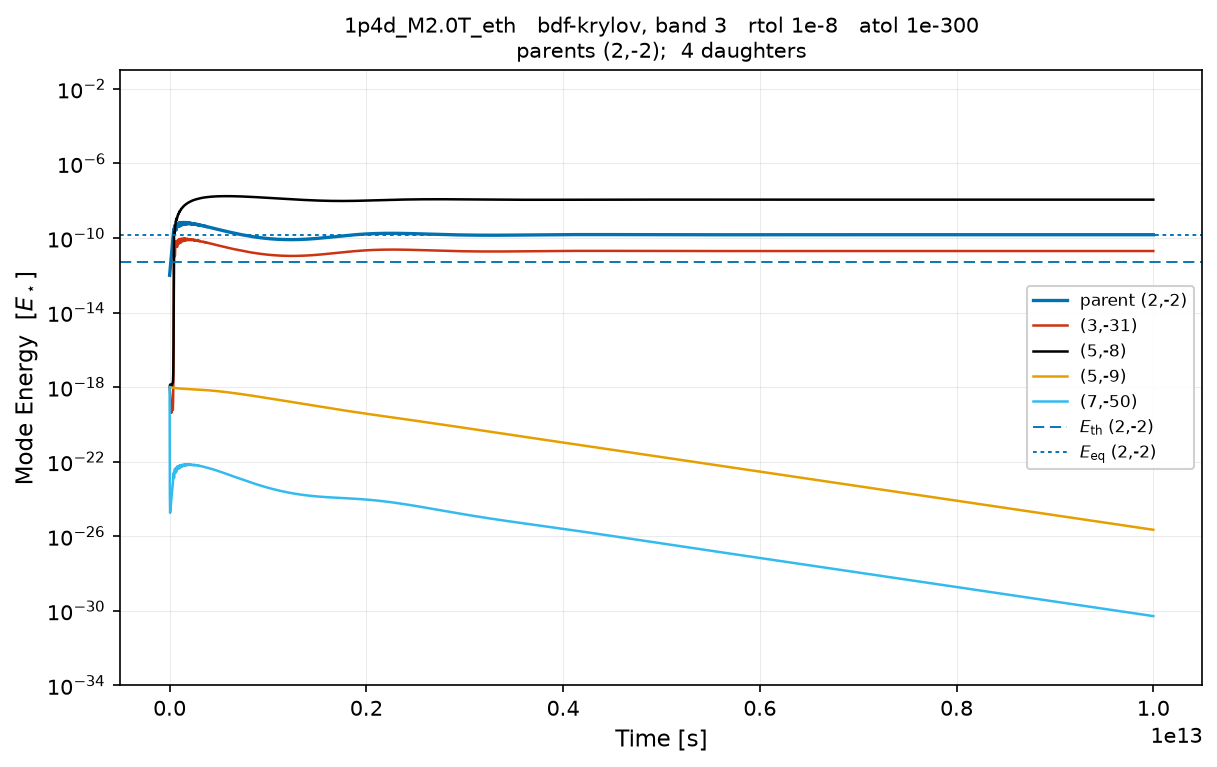
\includegraphics[width=0.21\textwidth,height=0.1323\textwidth]{../plots/krylov_b3/1p4d_M2.0T_eth/r1e-8_a1e-300.png} & 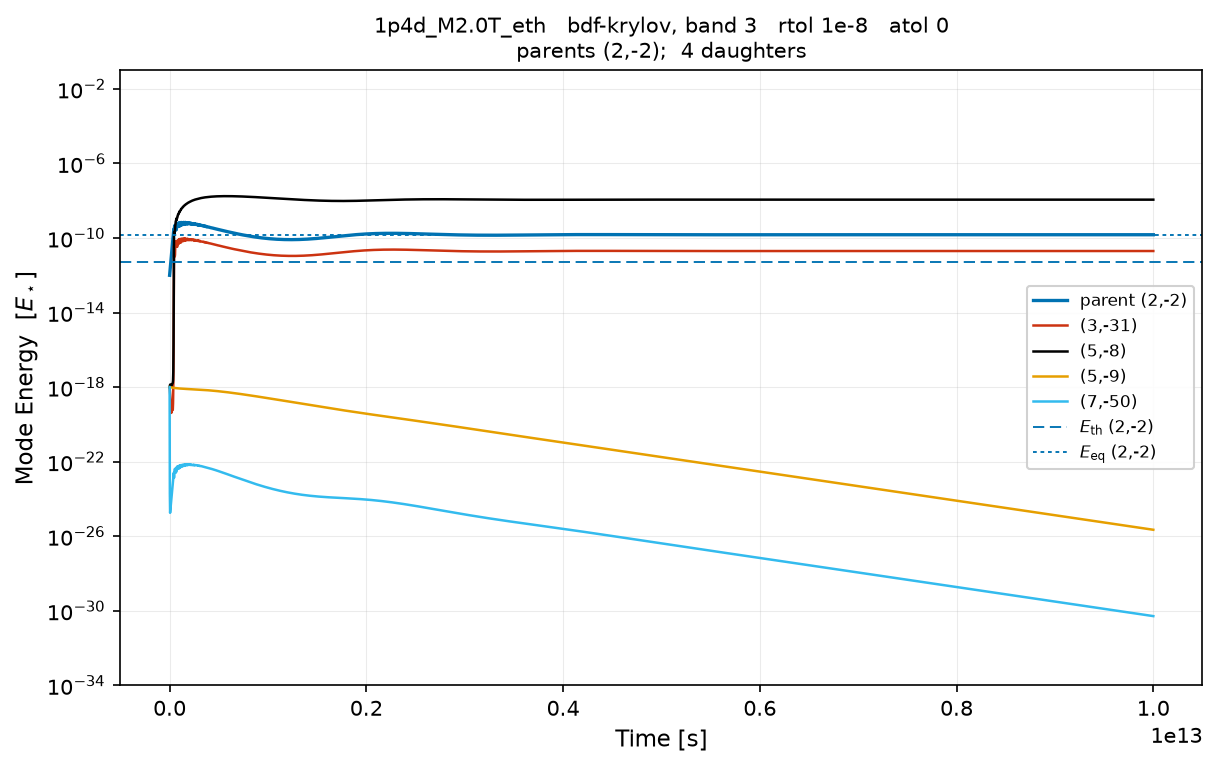
\includegraphics[width=0.21\textwidth,height=0.1323\textwidth]{../plots/krylov_b3/1p4d_M2.0T_eth/r1e-8_a0.png} \\[-1pt]
 & \parbox[t]{0.21\textwidth}{\centering\scriptsize 8.99\,M steps, 20.7\,s} & \parbox[t]{0.21\textwidth}{\centering\scriptsize 8.99\,M steps, 15.9\,s} & \parbox[t]{0.21\textwidth}{\centering\scriptsize 8.99\,M steps, 23.0\,s} & \parbox[t]{0.21\textwidth}{\centering\scriptsize 8.99\,M steps, 21.5\,s} \\[2pt]
\rotatebox{90}{\parbox{0.1323\textwidth}{\centering\scriptsize\bfseries Adams, fixed point}} & 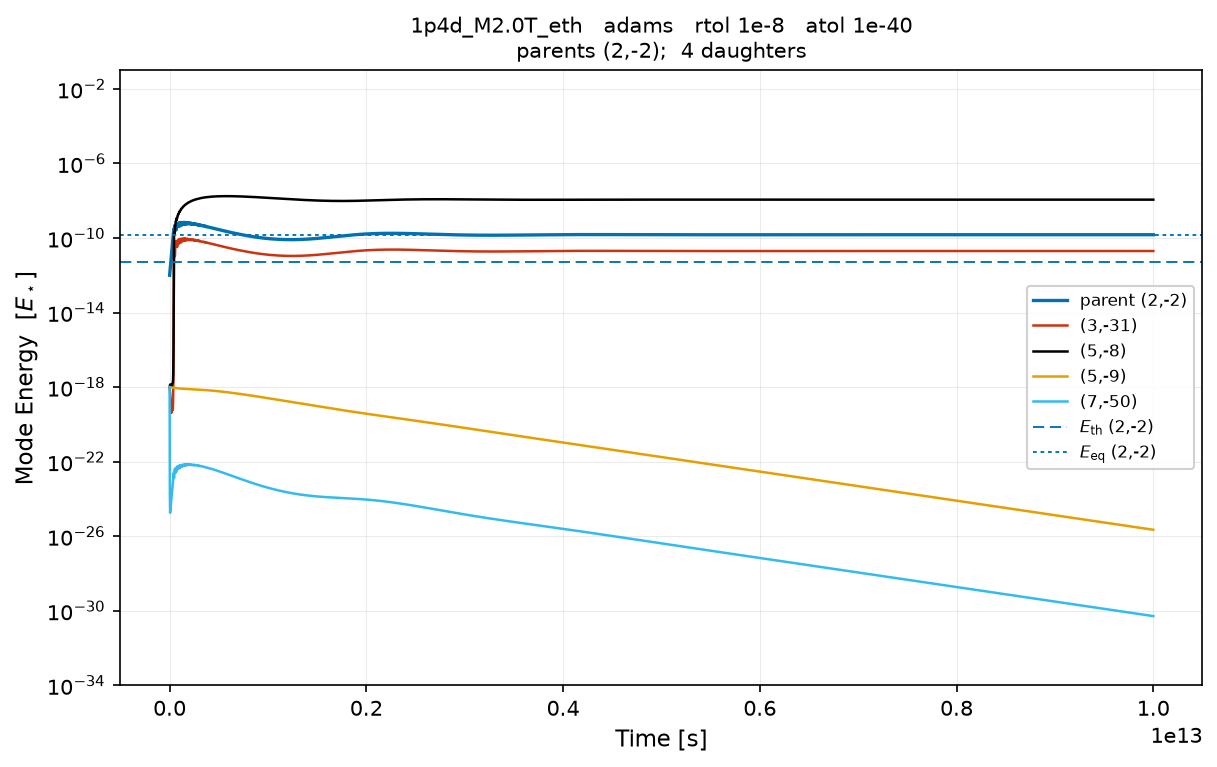
\includegraphics[width=0.21\textwidth,height=0.1323\textwidth]{../plots/adams/1p4d_M2.0T_eth/r1e-8_a1e-40.png} & 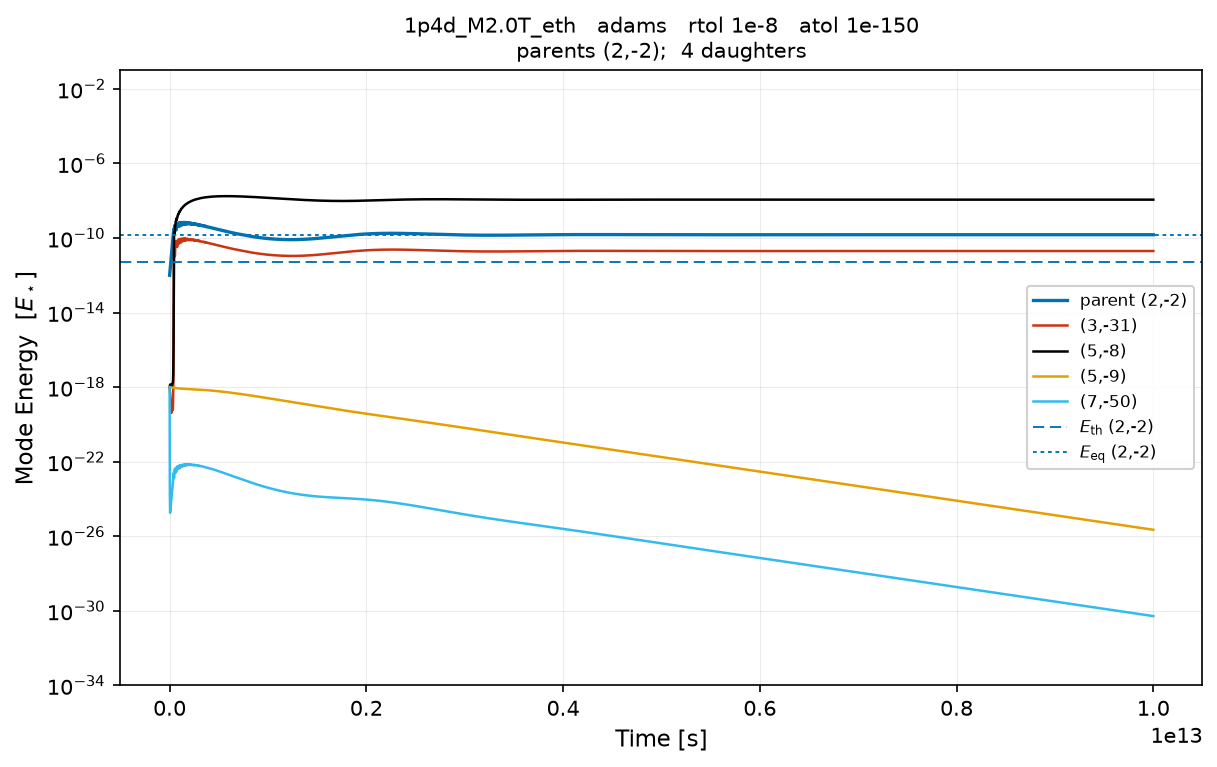
\includegraphics[width=0.21\textwidth,height=0.1323\textwidth]{../plots/adams/1p4d_M2.0T_eth/r1e-8_a1e-150.png} & 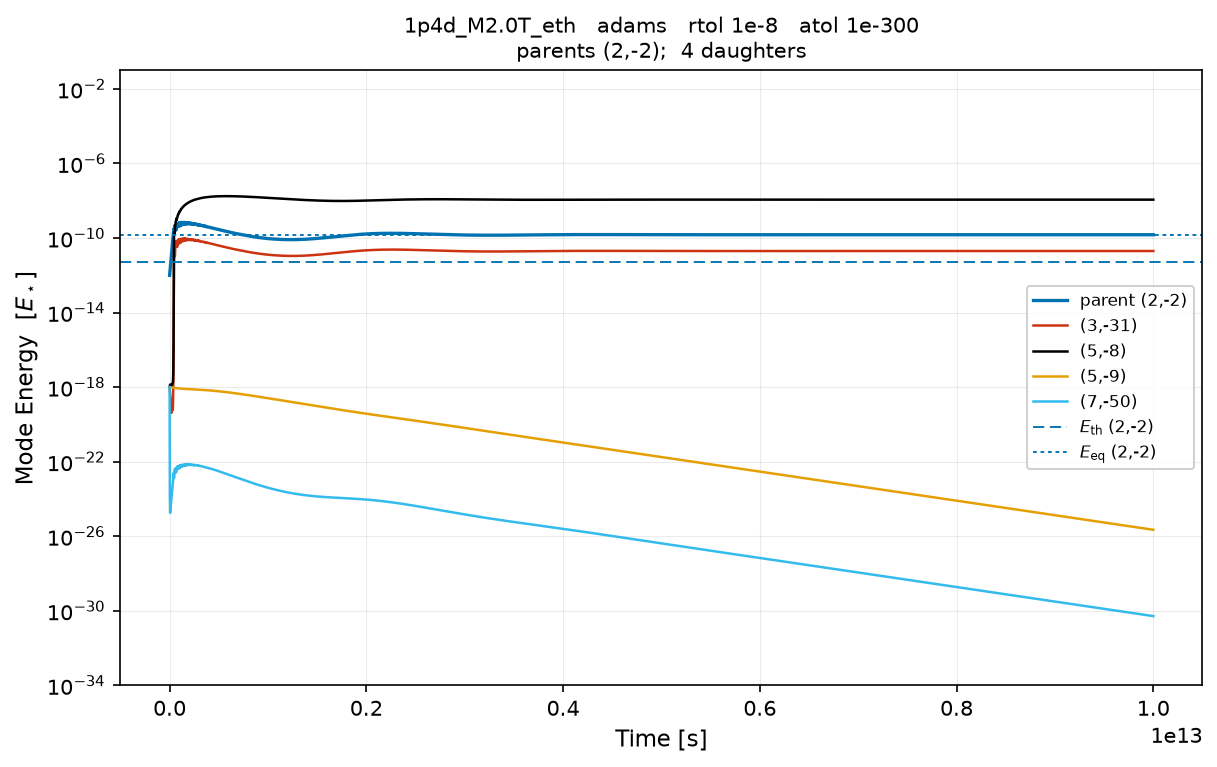
\includegraphics[width=0.21\textwidth,height=0.1323\textwidth]{../plots/adams/1p4d_M2.0T_eth/r1e-8_a1e-300.png} & 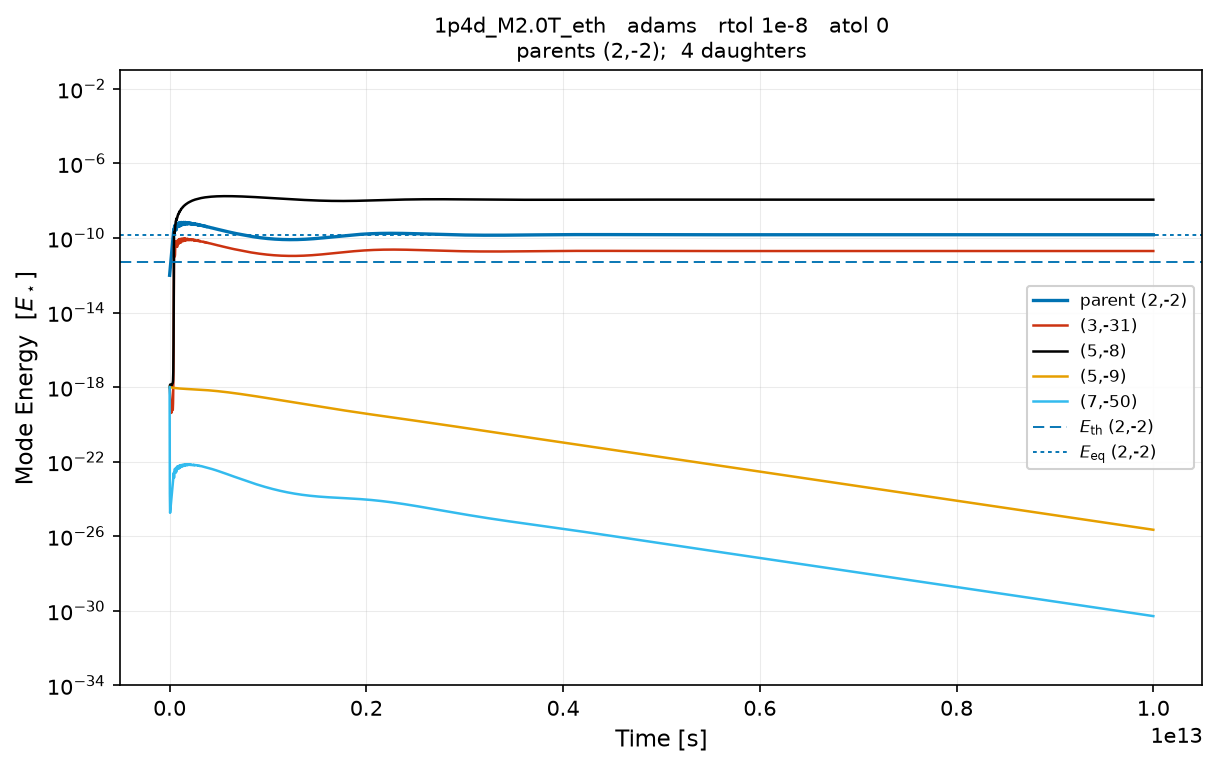
\includegraphics[width=0.21\textwidth,height=0.1323\textwidth]{../plots/adams/1p4d_M2.0T_eth/r1e-8_a0.png} \\[-1pt]
 & \parbox[t]{0.21\textwidth}{\centering\scriptsize 4.10\,M steps, 6.9\,s} & \parbox[t]{0.21\textwidth}{\centering\scriptsize 4.11\,M steps, 6.2\,s} & \parbox[t]{0.21\textwidth}{\centering\scriptsize 4.11\,M steps, 4.1\,s} & \parbox[t]{0.21\textwidth}{\centering\scriptsize 4.11\,M steps, 4.3\,s} \\[2pt]
\end{tabular}\par}
\par\noindent{\scriptsize\setlength\tabcolsep{3.5pt}\renewcommand\arraystretch{0.92}
\begin{tabular}{@{}llllrrrrrrr@{}}
\toprule
integrator & atol & stop & $t_{\rm stop}$ [s] & steps & rejected & RHS & Jac. & NL it. & lin. it. & wall [s] \\
\midrule
rk8pd & $10^{-40}$ & end & $1.00\times10^{13}$ & 618.4\,k & 18.4\,k & 8.04\,M & -- & -- & -- & 1.8 \\
 & $10^{-150}$ & end & $1.00\times10^{13}$ & 618.5\,k & 18.4\,k & 8.04\,M & -- & -- & -- & 2.5 \\
 & $10^{-300}$ & end & $1.00\times10^{13}$ & 618.5\,k & 18.4\,k & 8.04\,M & -- & -- & -- & 1.2 \\
 & $0$ & end & $1.00\times10^{13}$ & 618.5\,k & 18.4\,k & 8.04\,M & -- & -- & -- & 2.7 \\
\addlinespace[2pt]
BDF, dense analytic Jacobian & $10^{-40}$ & end & $1.00\times10^{13}$ & 9.43\,M & 89.6\,k & 10.13\,M & 167.6\,k & 10.13\,M & -- & 8.3 \\
 & $10^{-150}$ & end & $1.00\times10^{13}$ & 9.42\,M & 89.5\,k & 10.12\,M & 167.4\,k & 10.12\,M & -- & 9.5 \\
 & $10^{-300}$ & end & $1.00\times10^{13}$ & 9.42\,M & 89.5\,k & 10.12\,M & 167.4\,k & 10.12\,M & -- & 9.7 \\
 & $0$ & end & $1.00\times10^{13}$ & 9.42\,M & 89.5\,k & 10.12\,M & 167.4\,k & 10.12\,M & -- & 11.1 \\
\addlinespace[2pt]
BDF-Krylov, band full & $10^{-40}$ & end & $1.00\times10^{13}$ & 9.43\,M & 89.3\,k & 21.30\,M & 167.6\,k & 10.12\,M & 9.49\,M & 23.2 \\
 & $10^{-150}$ & end & $1.00\times10^{13}$ & 9.43\,M & 89.6\,k & 21.29\,M & 167.5\,k & 10.12\,M & 9.49\,M & 23.7 \\
 & $10^{-300}$ & end & $1.00\times10^{13}$ & 9.43\,M & 89.6\,k & 21.29\,M & 167.5\,k & 10.12\,M & 9.49\,M & 13.0 \\
 & $0$ & end & $1.00\times10^{13}$ & 9.43\,M & 89.6\,k & 21.29\,M & 167.5\,k & 10.12\,M & 9.49\,M & 14.4 \\
\addlinespace[2pt]
BDF-Krylov, band 3 & $10^{-40}$ & end & $1.00\times10^{13}$ & 8.99\,M & 122.0\,k & 21.67\,M & 160.4\,k & 9.86\,M & 10.69\,M & 20.7 \\
 & $10^{-150}$ & end & $1.00\times10^{13}$ & 8.99\,M & 122.3\,k & 21.67\,M & 160.4\,k & 9.86\,M & 10.68\,M & 15.9 \\
 & $10^{-300}$ & end & $1.00\times10^{13}$ & 8.99\,M & 122.3\,k & 21.67\,M & 160.4\,k & 9.86\,M & 10.68\,M & 23.0 \\
 & $0$ & end & $1.00\times10^{13}$ & 8.99\,M & 122.3\,k & 21.67\,M & 160.4\,k & 9.86\,M & 10.68\,M & 21.5 \\
\addlinespace[2pt]
Adams, fixed point & $10^{-40}$ & end & $1.00\times10^{13}$ & 4.10\,M & 287.6\,k & 6.43\,M & -- & 6.42\,M & -- & 6.9 \\
 & $10^{-150}$ & end & $1.00\times10^{13}$ & 4.11\,M & 283.9\,k & 6.44\,M & -- & 6.44\,M & -- & 6.2 \\
 & $10^{-300}$ & end & $1.00\times10^{13}$ & 4.11\,M & 283.9\,k & 6.44\,M & -- & 6.44\,M & -- & 4.1 \\
 & $0$ & end & $1.00\times10^{13}$ & 4.11\,M & 283.9\,k & 6.44\,M & -- & 6.44\,M & -- & 4.3 \\
\bottomrule
\end{tabular}}

\clearpage
\subsection{\texttt{1p4d\_M2.0\_eth}}\label{net:1p4d_M2.0_eth}
\noindent\begin{minipage}[t]{0.43\textwidth}\vspace{0pt}\footnotesize
\begin{tabular}{@{}rrlrr@{}}
\toprule
id & gen & $(\ell,n)$ & $\omega$ [rad\,s$^{-1}$] & $\gamma$ [s$^{-1}$] \\
\midrule
0 & 0 & (1,$-$1) & $7.581\times10^{-4}$ & $-2.276\times10^{-10}$ \\
1 & 1 & (4,$-$38) & $1.383\times10^{-4}$ & $2.224\times10^{-10}$ \\
2 & 1 & (5,$-$9) & $6.198\times10^{-4}$ & $4.584\times10^{-13}$ \\
3 & 1 & (4,$-$8) & $5.844\times10^{-4}$ & $4.902\times10^{-13}$ \\
4 & 1 & (5,$-$37) & $1.736\times10^{-4}$ & $1.454\times10^{-10}$ \\
\bottomrule
\end{tabular}
\end{minipage}\hfill
\begin{minipage}[t]{0.55\textwidth}\vspace{0pt}\footnotesize
\textbf{Model} \texttt{dsct\_M2.0}, rule eth, $N=4$, cut 0.15,
closure 0.005; 5 modes, 2 triplet(s).\\[2pt]
\textbf{Selecting pairs}\\ (1,$-$1) $\to$ (4,$-$38) + (5,$-$9): $\Delta/\omega_a=6.73\times10^{-5}$, $\kappa=+0.342$, $E_{\rm th}=1.33\times10^{-10}$, no $E_{\rm eq}$\\
(1,$-$1) $\to$ (4,$-$8) + (5,$-$37): $\Delta/\omega_a=-1.23\times10^{-4}$, $\kappa=+0.171$, $E_{\rm th}=2.46\times10^{-9}$, no $E_{\rm eq}$\\[2pt]

\end{minipage}

\par\smallskip{\centering\begin{tabular}{@{}c@{\hspace{2pt}}c@{\hspace{2pt}}c@{\hspace{2pt}}c@{\hspace{2pt}}c@{}}
 & \small atol $10^{-40}$ & \small atol $10^{-150}$ & \small atol $10^{-300}$ & \small atol $0$ \\[1pt]
\rotatebox{90}{\parbox{0.1323\textwidth}{\centering\scriptsize\bfseries rk8pd}} & 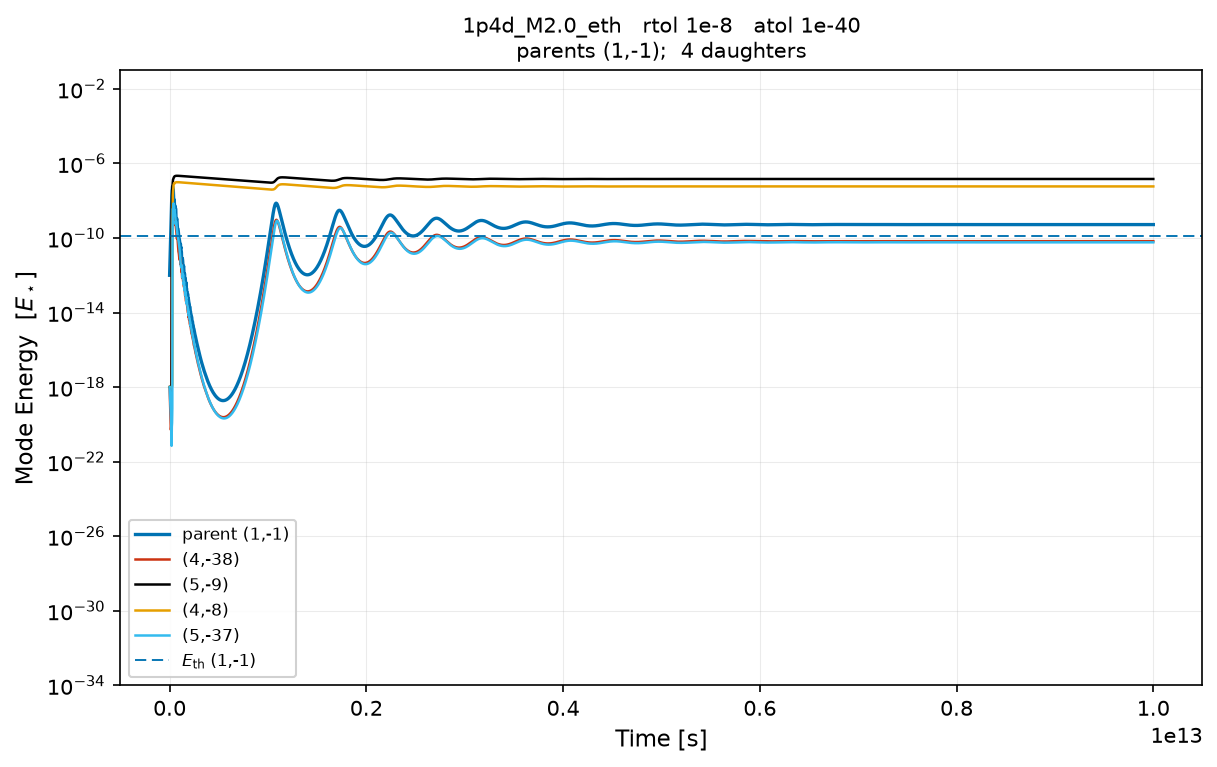
\includegraphics[width=0.21\textwidth,height=0.1323\textwidth]{../plots/rk8pd/1p4d_M2.0_eth/r1e-8_a1e-40.png} & 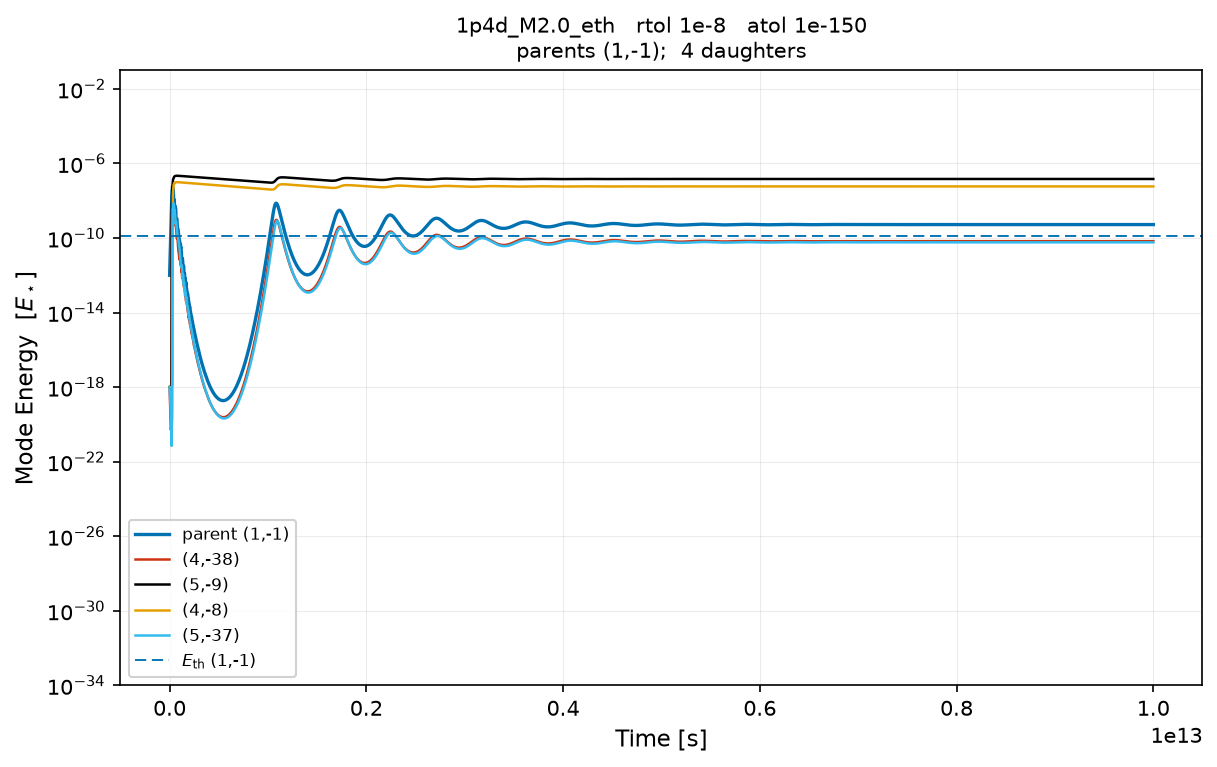
\includegraphics[width=0.21\textwidth,height=0.1323\textwidth]{../plots/rk8pd/1p4d_M2.0_eth/r1e-8_a1e-150.png} & 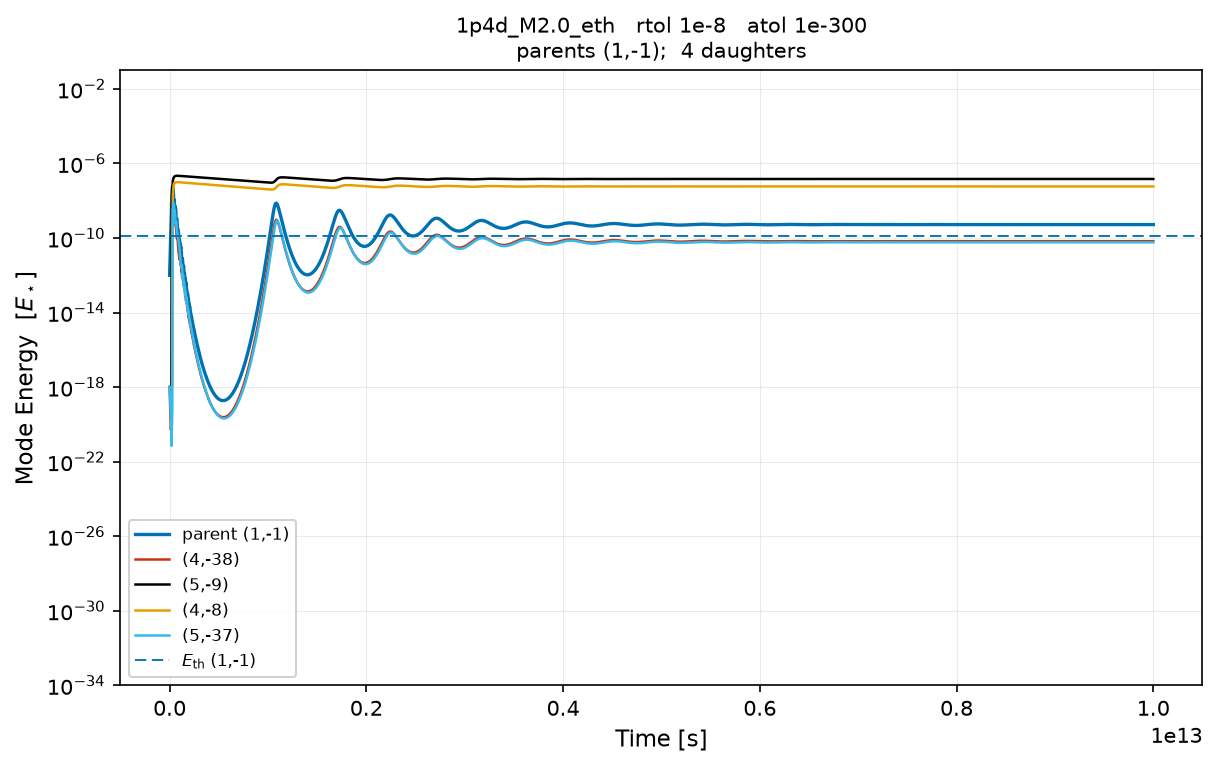
\includegraphics[width=0.21\textwidth,height=0.1323\textwidth]{../plots/rk8pd/1p4d_M2.0_eth/r1e-8_a1e-300.png} & 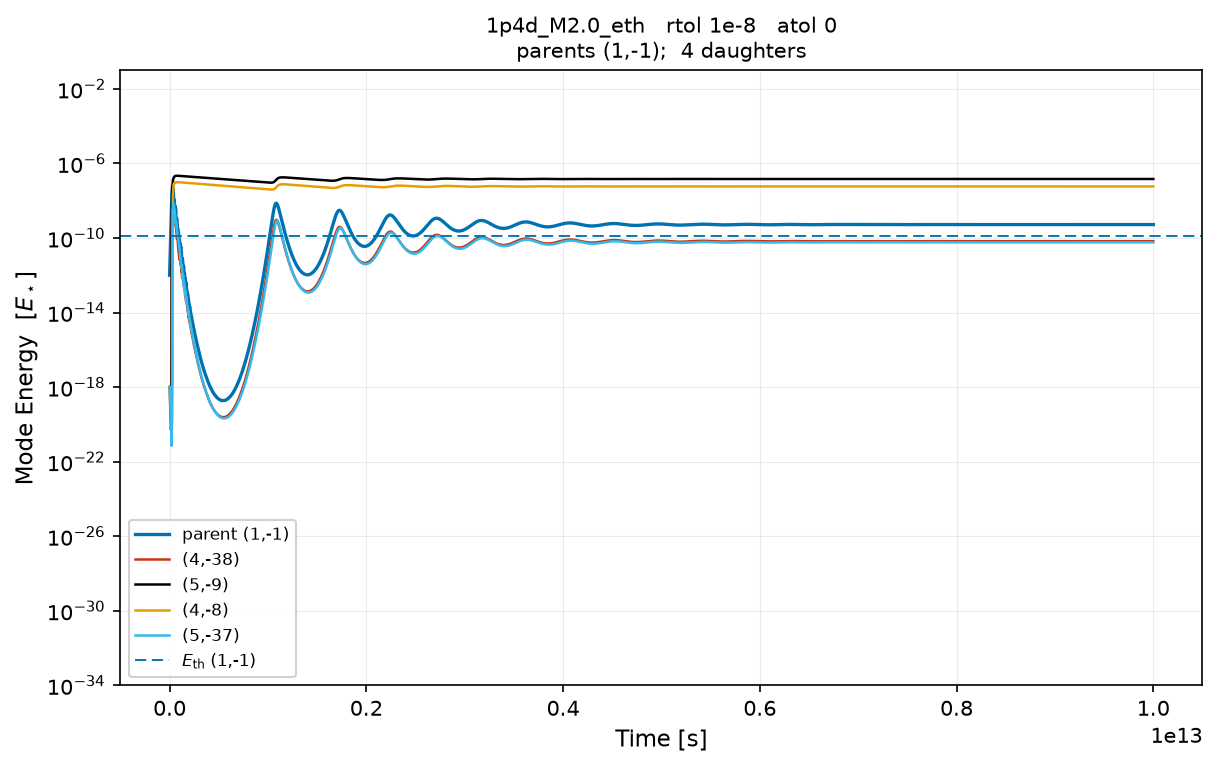
\includegraphics[width=0.21\textwidth,height=0.1323\textwidth]{../plots/rk8pd/1p4d_M2.0_eth/r1e-8_a0.png} \\[-1pt]
 & \parbox[t]{0.21\textwidth}{\centering\scriptsize 2.41\,M steps, 5.2\,s} & \parbox[t]{0.21\textwidth}{\centering\scriptsize 2.41\,M steps, 10.5\,s} & \parbox[t]{0.21\textwidth}{\centering\scriptsize 2.41\,M steps, 7.6\,s} & \parbox[t]{0.21\textwidth}{\centering\scriptsize 2.41\,M steps, 10.1\,s} \\[2pt]
\rotatebox{90}{\parbox{0.1323\textwidth}{\centering\scriptsize\bfseries BDF, dense analytic Jacobian}} & 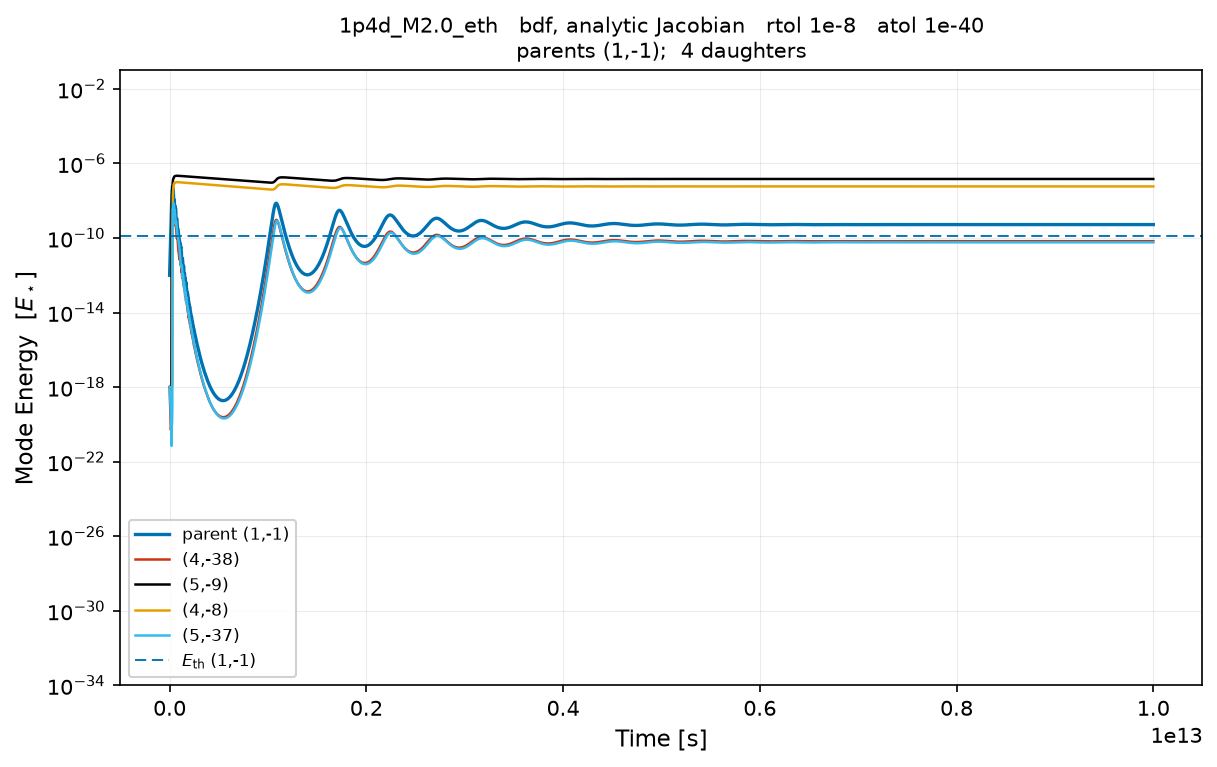
\includegraphics[width=0.21\textwidth,height=0.1323\textwidth]{../plots/bdf/1p4d_M2.0_eth/r1e-8_a1e-40.png} & 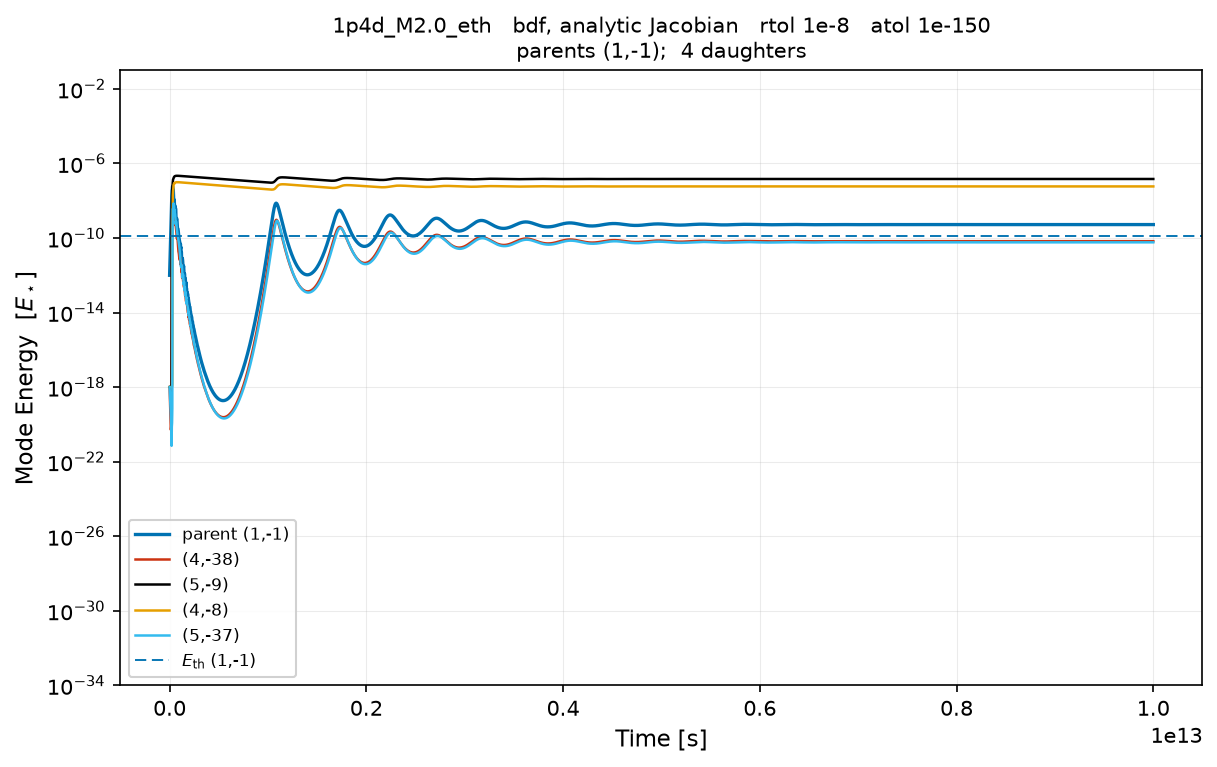
\includegraphics[width=0.21\textwidth,height=0.1323\textwidth]{../plots/bdf/1p4d_M2.0_eth/r1e-8_a1e-150.png} & 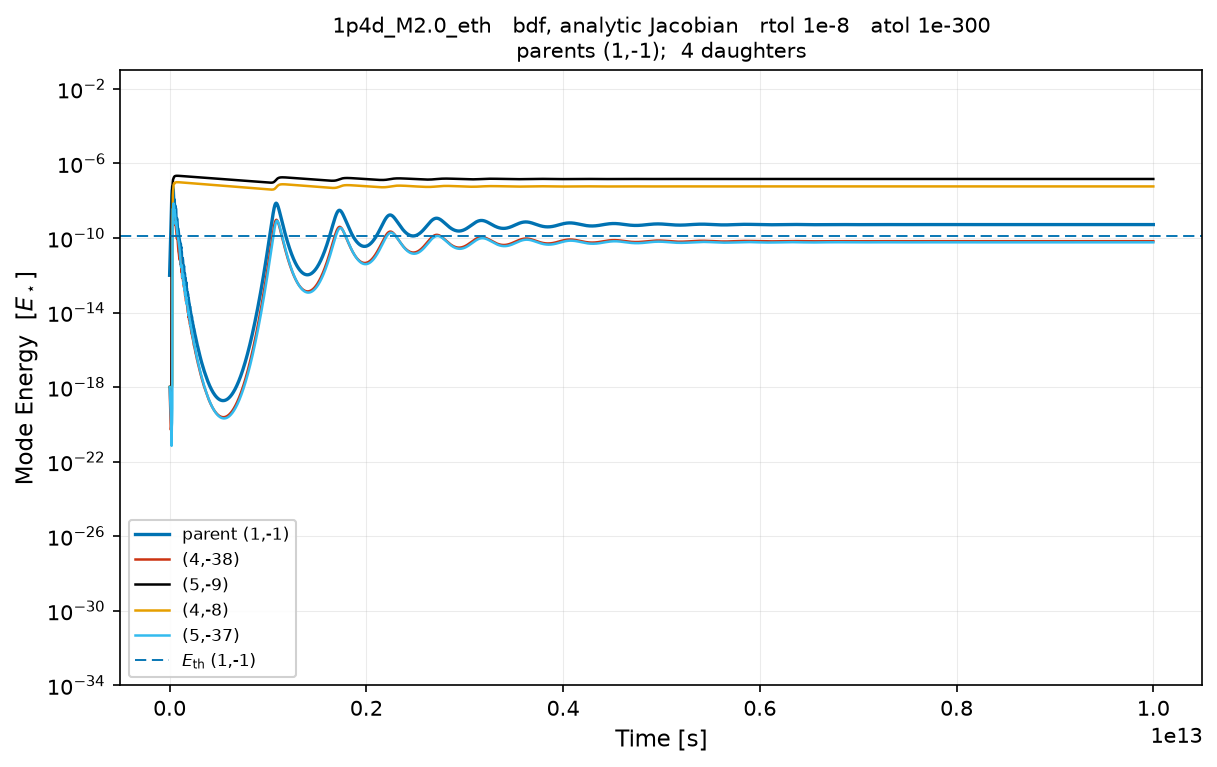
\includegraphics[width=0.21\textwidth,height=0.1323\textwidth]{../plots/bdf/1p4d_M2.0_eth/r1e-8_a1e-300.png} & 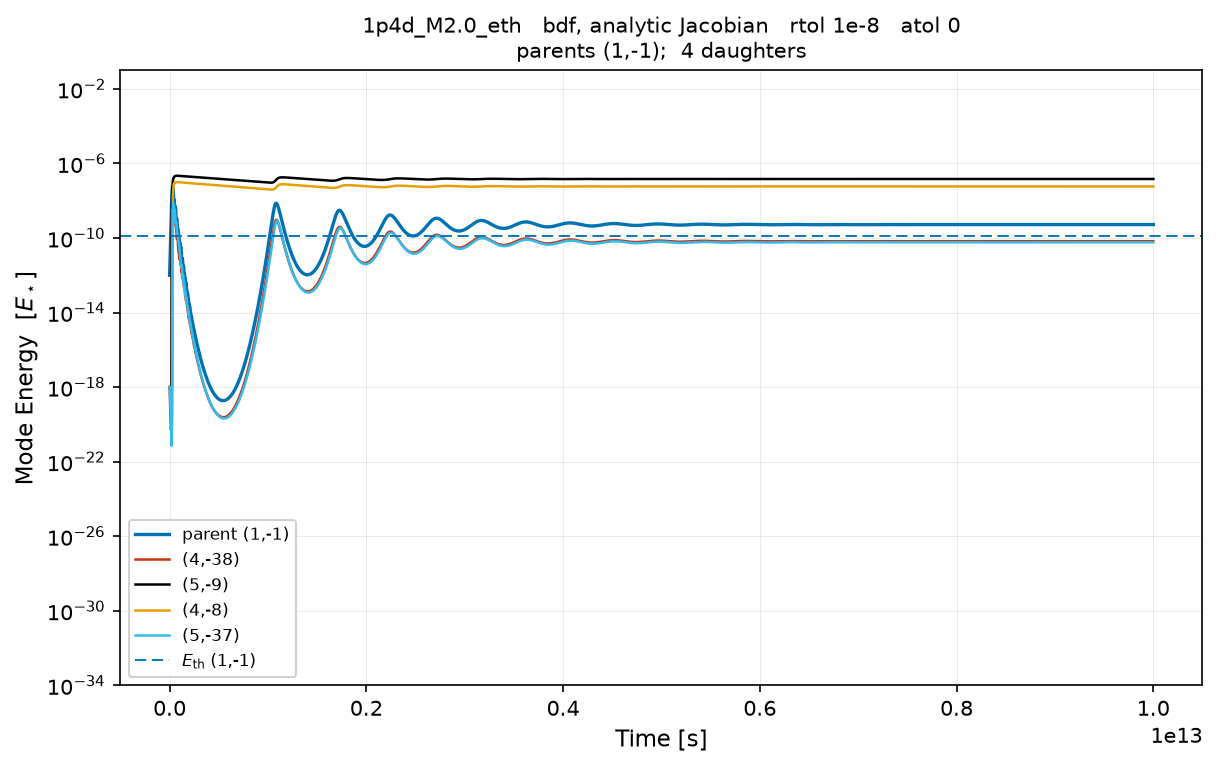
\includegraphics[width=0.21\textwidth,height=0.1323\textwidth]{../plots/bdf/1p4d_M2.0_eth/r1e-8_a0.png} \\[-1pt]
 & \parbox[t]{0.21\textwidth}{\centering\scriptsize 20.95\,M steps, 33.9\,s} & \parbox[t]{0.21\textwidth}{\centering\scriptsize 20.95\,M steps, 30.8\,s} & \parbox[t]{0.21\textwidth}{\centering\scriptsize 20.95\,M steps, 26.4\,s} & \parbox[t]{0.21\textwidth}{\centering\scriptsize 20.95\,M steps, 34.6\,s} \\[2pt]
\rotatebox{90}{\parbox{0.1323\textwidth}{\centering\scriptsize\bfseries BDF-Krylov, band full}} & 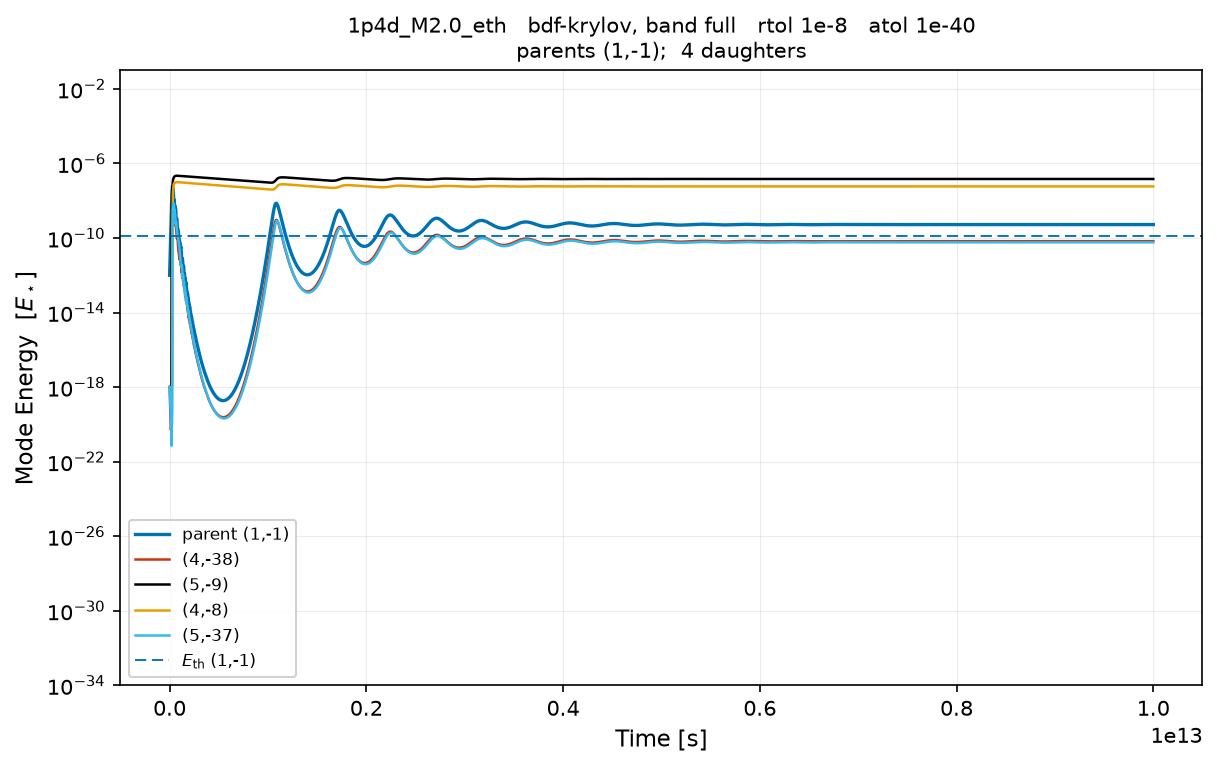
\includegraphics[width=0.21\textwidth,height=0.1323\textwidth]{../plots/krylov_full/1p4d_M2.0_eth/r1e-8_a1e-40.png} & 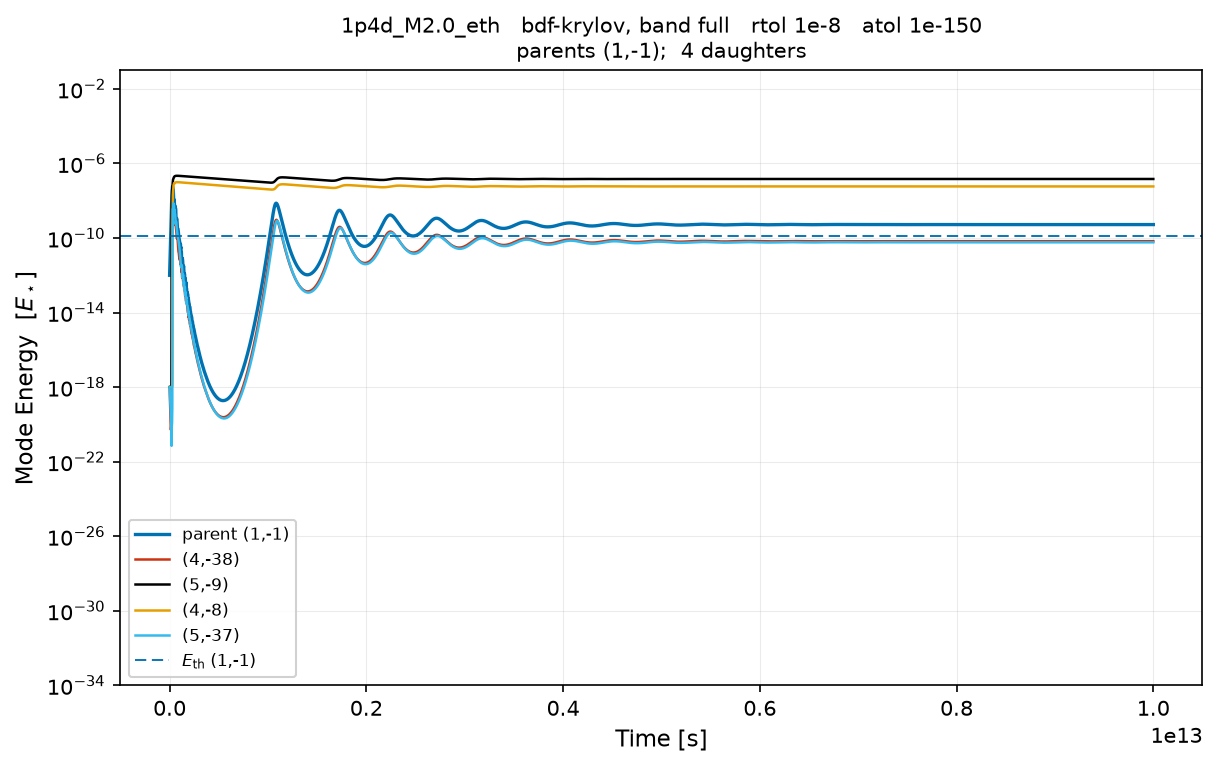
\includegraphics[width=0.21\textwidth,height=0.1323\textwidth]{../plots/krylov_full/1p4d_M2.0_eth/r1e-8_a1e-150.png} & 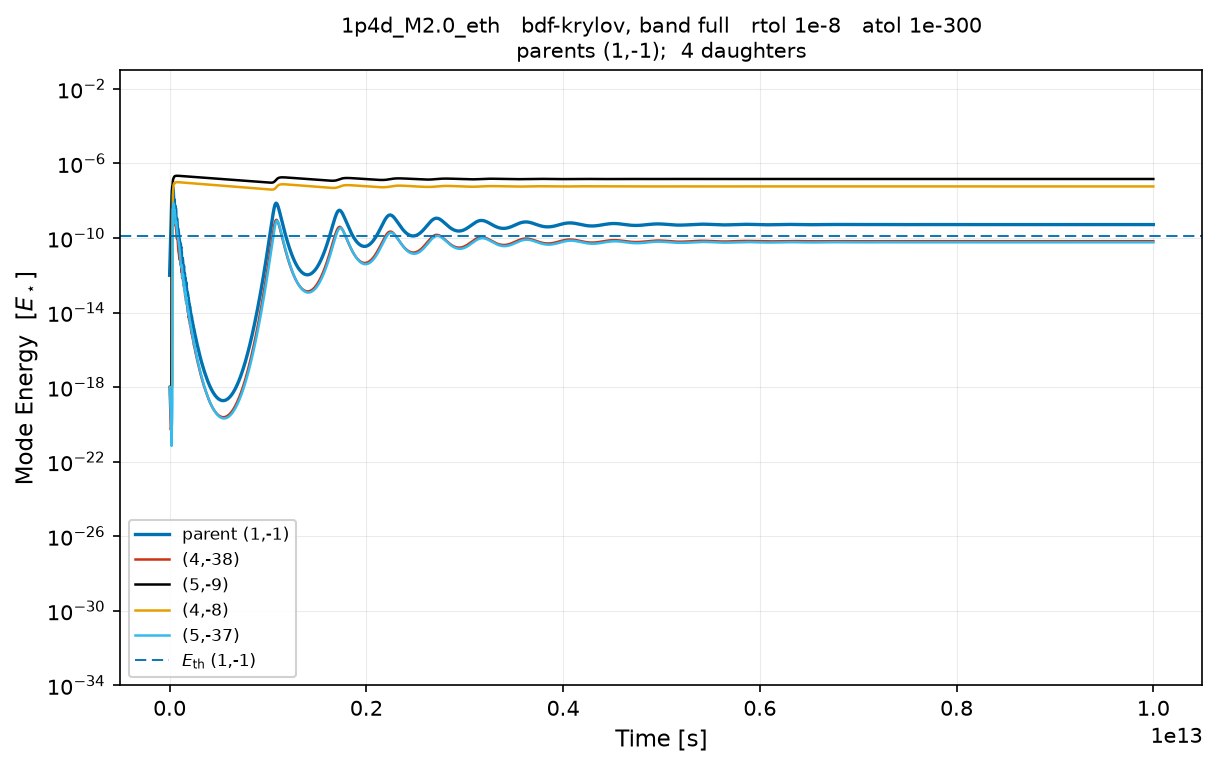
\includegraphics[width=0.21\textwidth,height=0.1323\textwidth]{../plots/krylov_full/1p4d_M2.0_eth/r1e-8_a1e-300.png} & 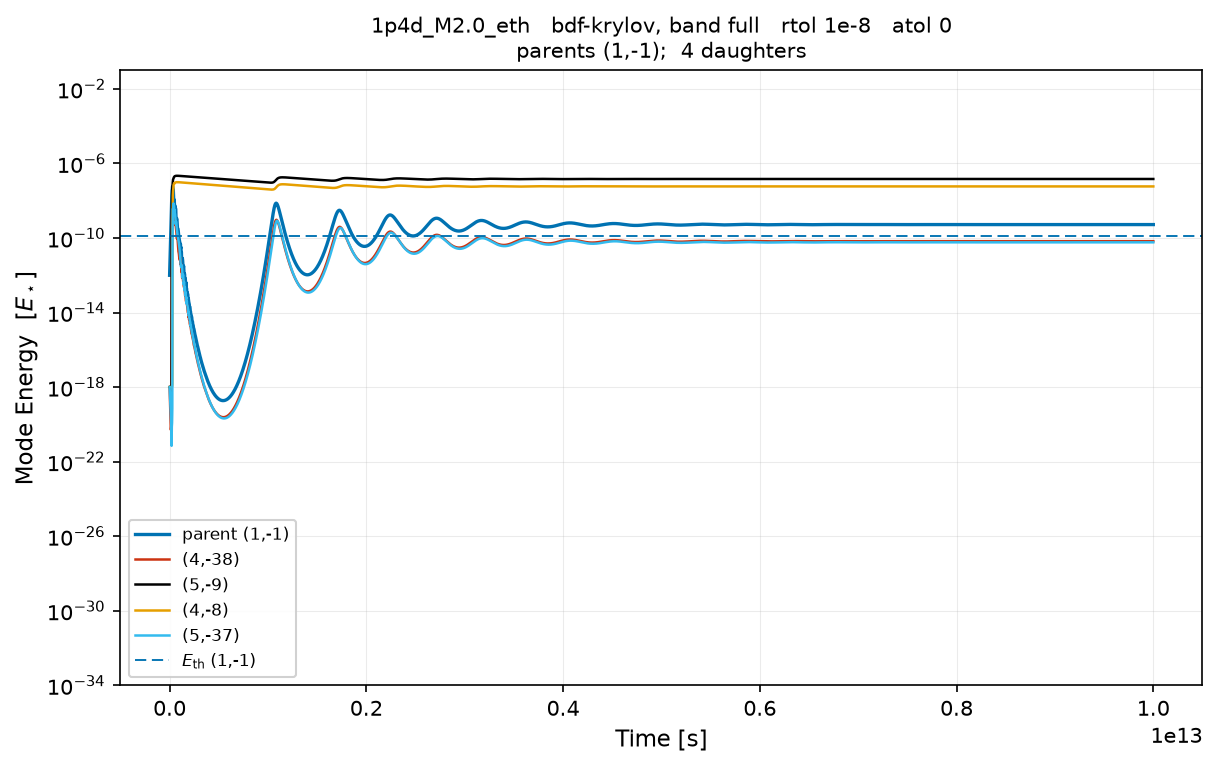
\includegraphics[width=0.21\textwidth,height=0.1323\textwidth]{../plots/krylov_full/1p4d_M2.0_eth/r1e-8_a0.png} \\[-1pt]
 & \parbox[t]{0.21\textwidth}{\centering\scriptsize 19.99\,M steps, 29.7\,s} & \parbox[t]{0.21\textwidth}{\centering\scriptsize 19.99\,M steps, 50.6\,s} & \parbox[t]{0.21\textwidth}{\centering\scriptsize 19.99\,M steps, 28.5\,s} & \parbox[t]{0.21\textwidth}{\centering\scriptsize 19.99\,M steps, 49.4\,s} \\[2pt]
\rotatebox{90}{\parbox{0.1323\textwidth}{\centering\scriptsize\bfseries BDF-Krylov, band 3}} & 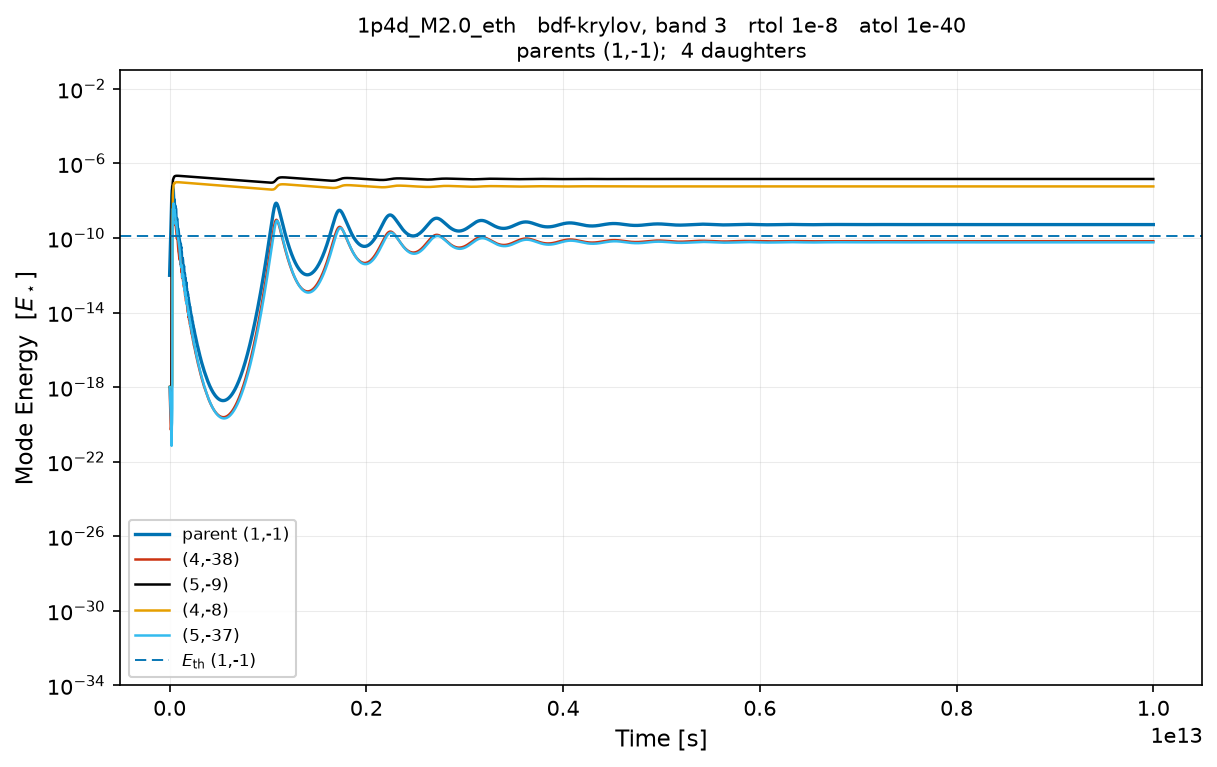
\includegraphics[width=0.21\textwidth,height=0.1323\textwidth]{../plots/krylov_b3/1p4d_M2.0_eth/r1e-8_a1e-40.png} & 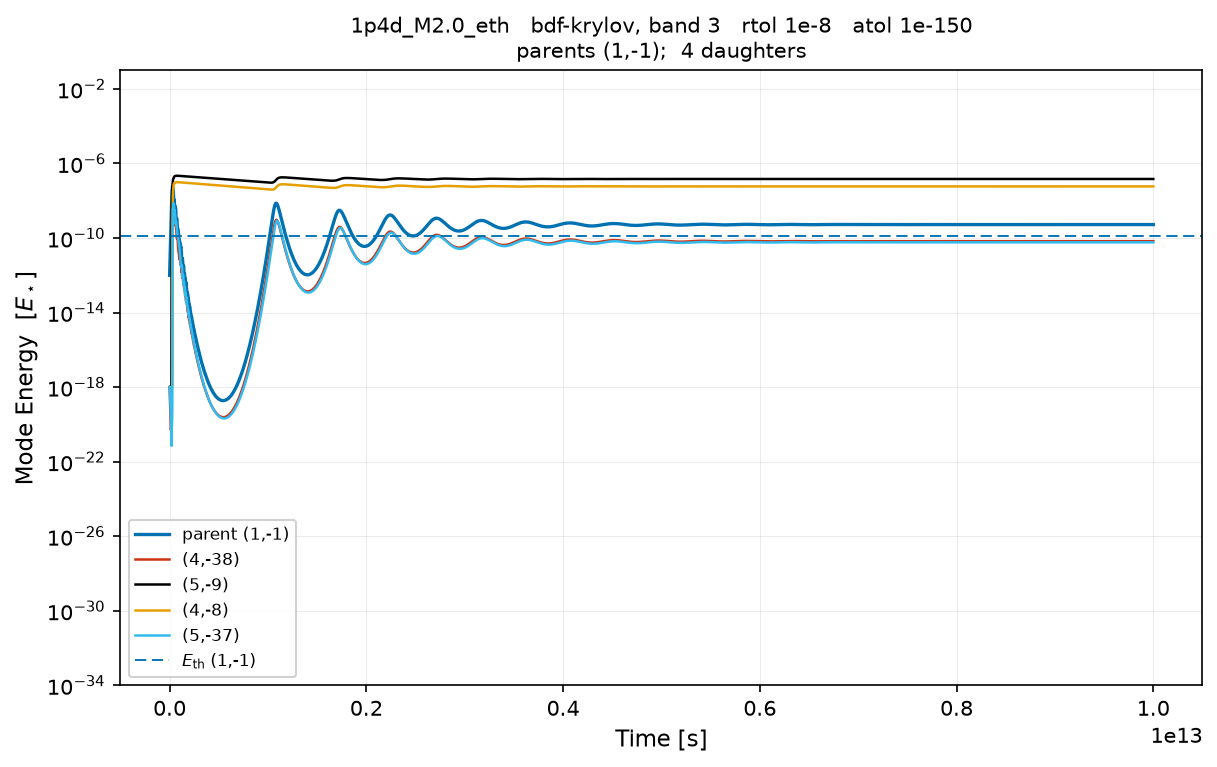
\includegraphics[width=0.21\textwidth,height=0.1323\textwidth]{../plots/krylov_b3/1p4d_M2.0_eth/r1e-8_a1e-150.png} & 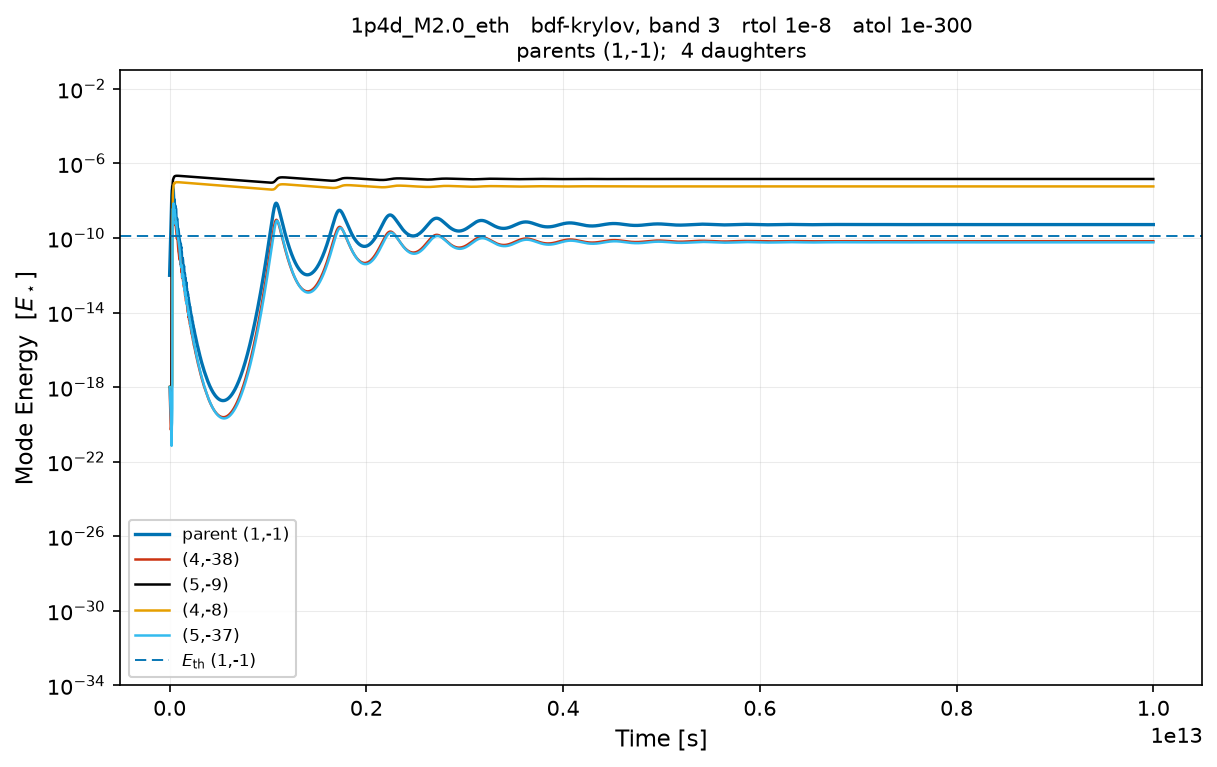
\includegraphics[width=0.21\textwidth,height=0.1323\textwidth]{../plots/krylov_b3/1p4d_M2.0_eth/r1e-8_a1e-300.png} & 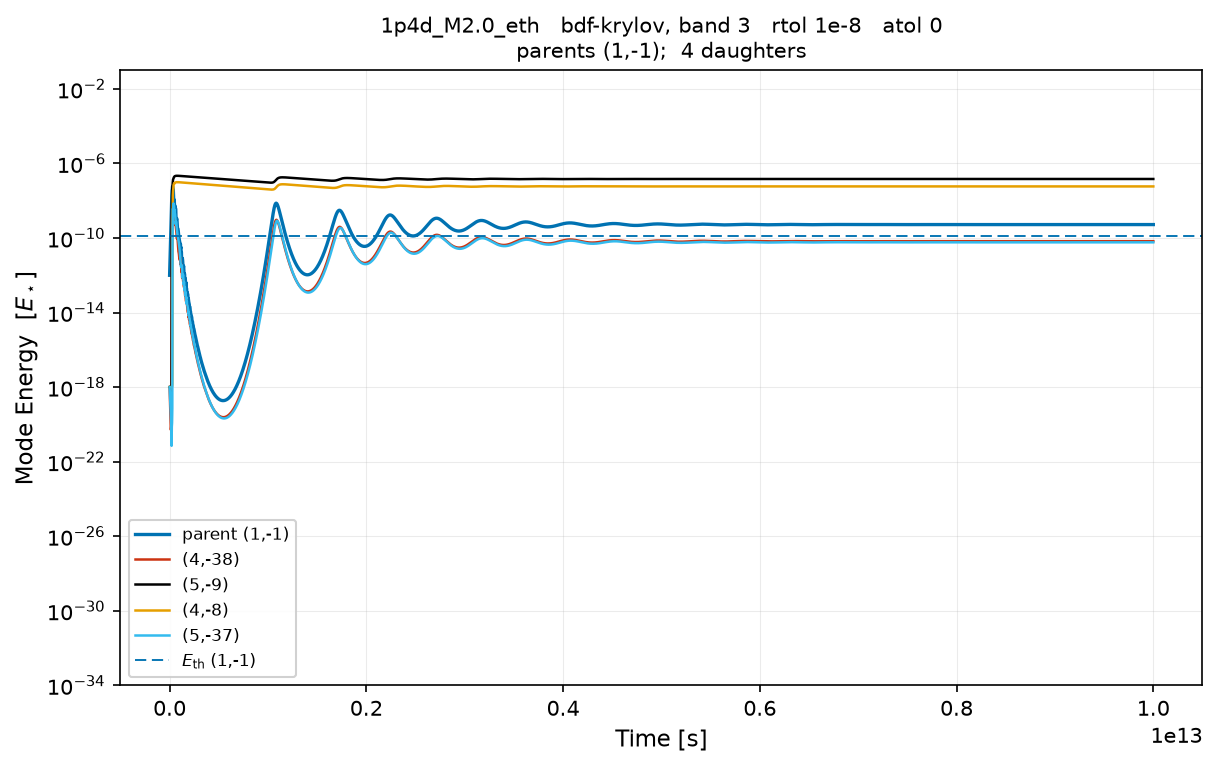
\includegraphics[width=0.21\textwidth,height=0.1323\textwidth]{../plots/krylov_b3/1p4d_M2.0_eth/r1e-8_a0.png} \\[-1pt]
 & \parbox[t]{0.21\textwidth}{\centering\scriptsize 19.90\,M steps, 30.2\,s} & \parbox[t]{0.21\textwidth}{\centering\scriptsize 19.89\,M steps, 50.7\,s} & \parbox[t]{0.21\textwidth}{\centering\scriptsize 19.89\,M steps, 35.2\,s} & \parbox[t]{0.21\textwidth}{\centering\scriptsize 19.89\,M steps, 36.8\,s} \\[2pt]
\rotatebox{90}{\parbox{0.1323\textwidth}{\centering\scriptsize\bfseries Adams, fixed point}} & 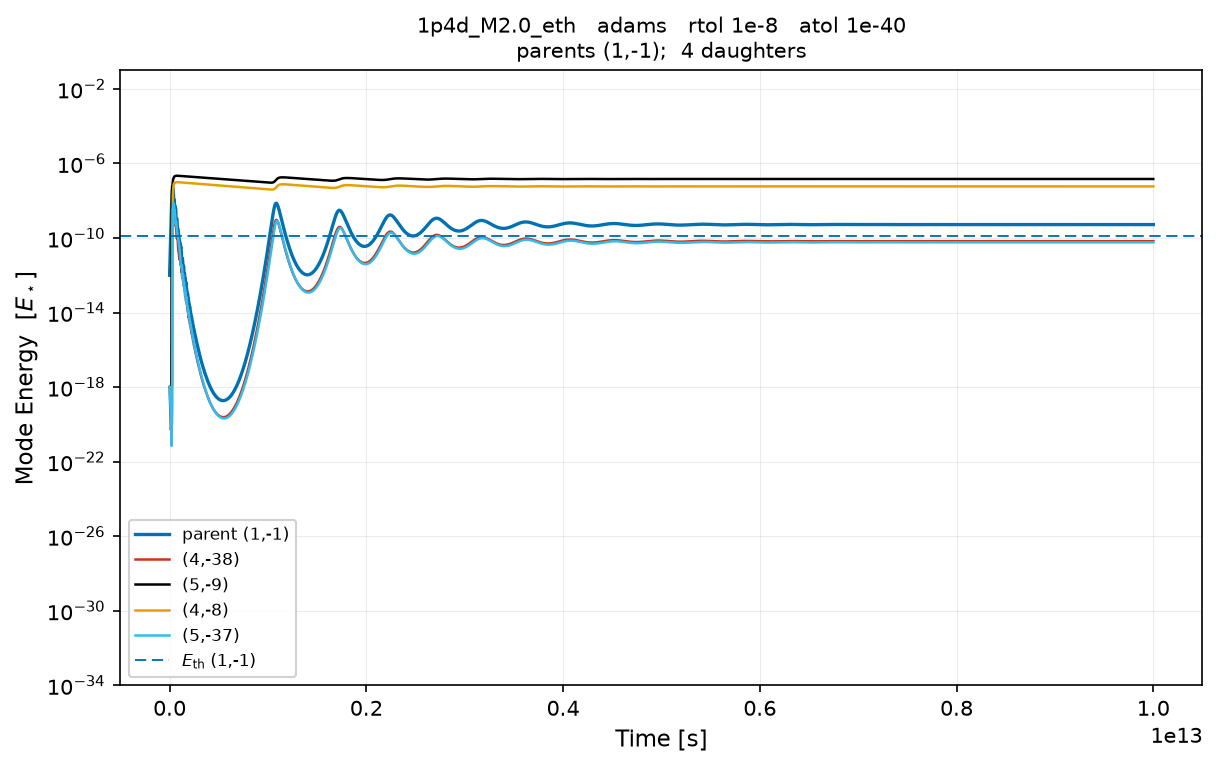
\includegraphics[width=0.21\textwidth,height=0.1323\textwidth]{../plots/adams/1p4d_M2.0_eth/r1e-8_a1e-40.png} & 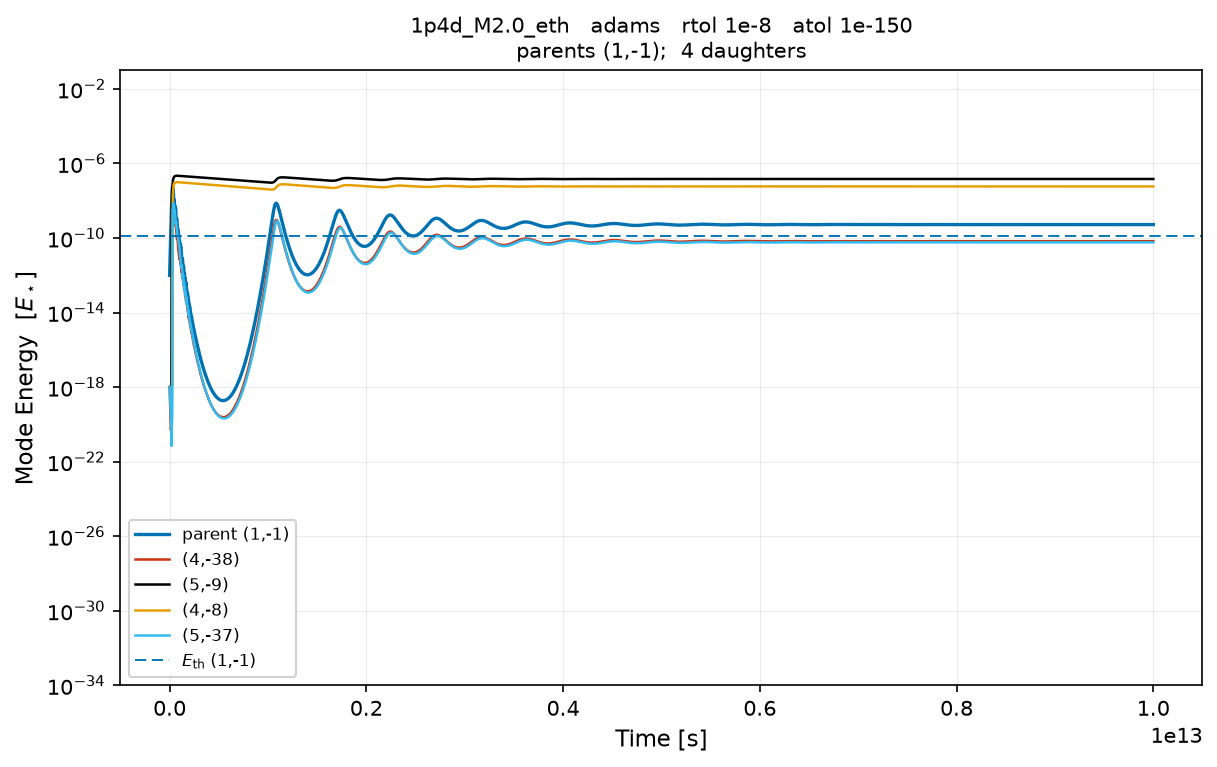
\includegraphics[width=0.21\textwidth,height=0.1323\textwidth]{../plots/adams/1p4d_M2.0_eth/r1e-8_a1e-150.png} & 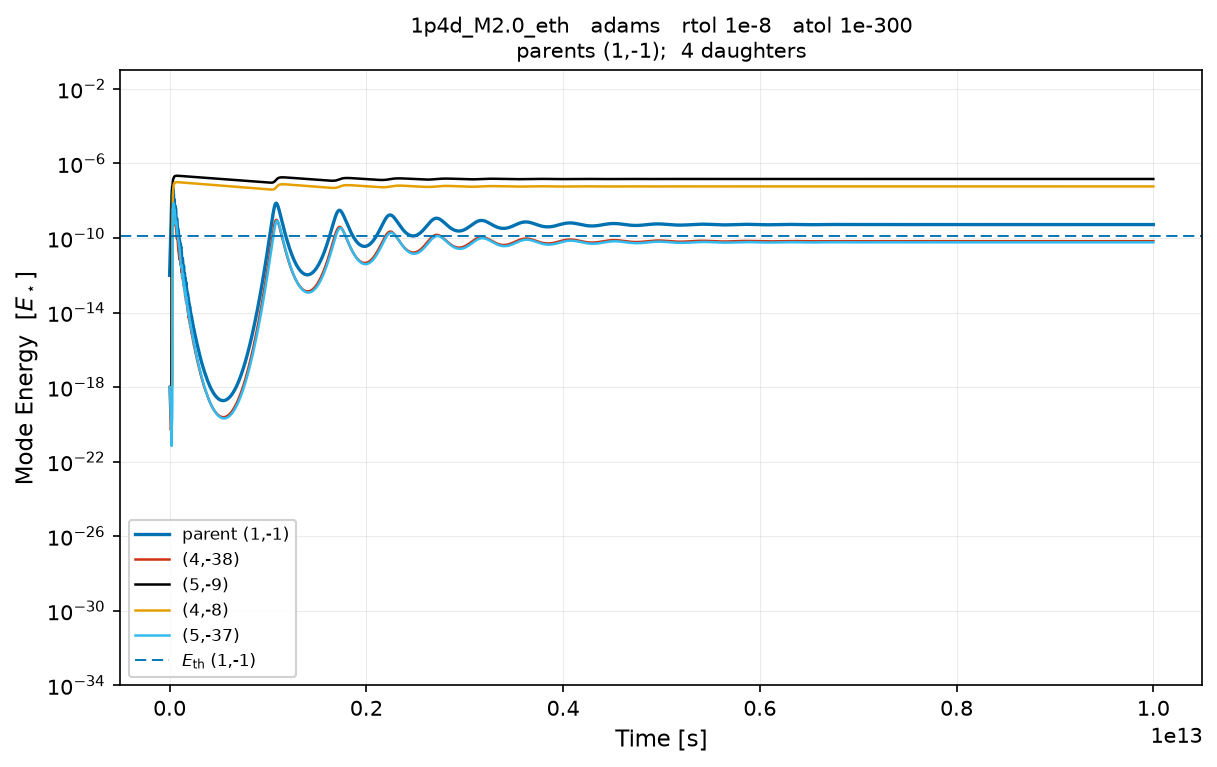
\includegraphics[width=0.21\textwidth,height=0.1323\textwidth]{../plots/adams/1p4d_M2.0_eth/r1e-8_a1e-300.png} & 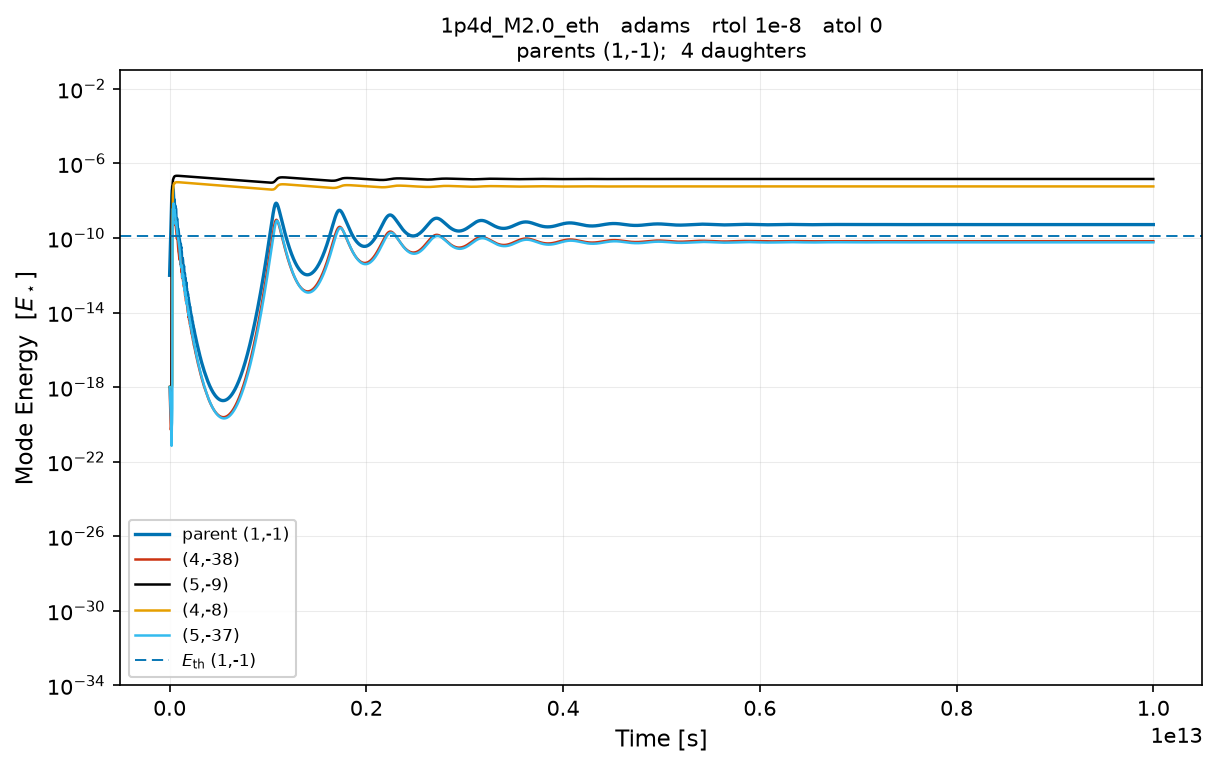
\includegraphics[width=0.21\textwidth,height=0.1323\textwidth]{../plots/adams/1p4d_M2.0_eth/r1e-8_a0.png} \\[-1pt]
 & \parbox[t]{0.21\textwidth}{\centering\scriptsize 12.04\,M steps, 18.8\,s} & \parbox[t]{0.21\textwidth}{\centering\scriptsize 12.04\,M steps, 15.4\,s} & \parbox[t]{0.21\textwidth}{\centering\scriptsize 12.04\,M steps, 18.5\,s} & \parbox[t]{0.21\textwidth}{\centering\scriptsize 12.04\,M steps, 11.4\,s} \\[2pt]
\end{tabular}\par}
\par\noindent{\scriptsize\setlength\tabcolsep{3.5pt}\renewcommand\arraystretch{0.92}
\begin{tabular}{@{}llllrrrrrrr@{}}
\toprule
integrator & atol & stop & $t_{\rm stop}$ [s] & steps & rejected & RHS & Jac. & NL it. & lin. it. & wall [s] \\
\midrule
rk8pd & $10^{-40}$ & end & $1.00\times10^{13}$ & 2.41\,M & 469.8\,k & 31.29\,M & -- & -- & -- & 5.2 \\
 & $10^{-150}$ & end & $1.00\times10^{13}$ & 2.41\,M & 469.8\,k & 31.29\,M & -- & -- & -- & 10.5 \\
 & $10^{-300}$ & end & $1.00\times10^{13}$ & 2.41\,M & 469.8\,k & 31.29\,M & -- & -- & -- & 7.6 \\
 & $0$ & end & $1.00\times10^{13}$ & 2.41\,M & 469.8\,k & 31.29\,M & -- & -- & -- & 10.1 \\
\addlinespace[2pt]
BDF, dense analytic Jacobian & $10^{-40}$ & end & $1.00\times10^{13}$ & 20.95\,M & 234.2\,k & 22.64\,M & 370.5\,k & 22.63\,M & -- & 33.9 \\
 & $10^{-150}$ & end & $1.00\times10^{13}$ & 20.95\,M & 234.2\,k & 22.64\,M & 370.5\,k & 22.63\,M & -- & 30.8 \\
 & $10^{-300}$ & end & $1.00\times10^{13}$ & 20.95\,M & 234.2\,k & 22.64\,M & 370.5\,k & 22.63\,M & -- & 26.4 \\
 & $0$ & end & $1.00\times10^{13}$ & 20.95\,M & 234.2\,k & 22.64\,M & 370.5\,k & 22.63\,M & -- & 34.6 \\
\addlinespace[2pt]
BDF-Krylov, band full & $10^{-40}$ & end & $1.00\times10^{13}$ & 19.99\,M & 229.1\,k & 47.20\,M & 345.1\,k & 21.71\,M & 22.04\,M & 29.7 \\
 & $10^{-150}$ & end & $1.00\times10^{13}$ & 19.99\,M & 229.1\,k & 47.20\,M & 345.1\,k & 21.71\,M & 22.04\,M & 50.6 \\
 & $10^{-300}$ & end & $1.00\times10^{13}$ & 19.99\,M & 229.1\,k & 47.20\,M & 345.1\,k & 21.71\,M & 22.04\,M & 28.5 \\
 & $0$ & end & $1.00\times10^{13}$ & 19.99\,M & 229.1\,k & 47.20\,M & 345.1\,k & 21.71\,M & 22.04\,M & 49.4 \\
\addlinespace[2pt]
BDF-Krylov, band 3 & $10^{-40}$ & end & $1.00\times10^{13}$ & 19.90\,M & 240.9\,k & 47.57\,M & 343.7\,k & 21.69\,M & 23.47\,M & 30.2 \\
 & $10^{-150}$ & end & $1.00\times10^{13}$ & 19.89\,M & 240.0\,k & 47.56\,M & 343.5\,k & 21.68\,M & 23.48\,M & 50.7 \\
 & $10^{-300}$ & end & $1.00\times10^{13}$ & 19.89\,M & 240.0\,k & 47.56\,M & 343.5\,k & 21.68\,M & 23.48\,M & 35.2 \\
 & $0$ & end & $1.00\times10^{13}$ & 19.89\,M & 240.0\,k & 47.56\,M & 343.5\,k & 21.68\,M & 23.48\,M & 36.8 \\
\addlinespace[2pt]
Adams, fixed point & $10^{-40}$ & end & $1.00\times10^{13}$ & 12.04\,M & 642.1\,k & 19.37\,M & -- & 19.36\,M & -- & 18.8 \\
 & $10^{-150}$ & end & $1.00\times10^{13}$ & 12.04\,M & 642.1\,k & 19.37\,M & -- & 19.36\,M & -- & 15.4 \\
 & $10^{-300}$ & end & $1.00\times10^{13}$ & 12.04\,M & 642.1\,k & 19.37\,M & -- & 19.36\,M & -- & 18.5 \\
 & $0$ & end & $1.00\times10^{13}$ & 12.04\,M & 642.1\,k & 19.37\,M & -- & 19.36\,M & -- & 11.4 \\
\bottomrule
\end{tabular}}

\clearpage
\subsection{\texttt{2p\_M1.7\_eth}}\label{net:2p_M1.7_eth}
\noindent\begin{minipage}[t]{0.43\textwidth}\vspace{0pt}\footnotesize
\begin{tabular}{@{}rrlrr@{}}
\toprule
id & gen & $(\ell,n)$ & $\omega$ [rad\,s$^{-1}$] & $\gamma$ [s$^{-1}$] \\
\midrule
0 & 0 & (1,+1) & $1.402\times10^{-3}$ & $-1.150\times10^{-10}$ \\
1 & 0 & (2,$-$3) & $8.582\times10^{-4}$ & $-3.458\times10^{-14}$ \\
2 & 1 & (6,$-$6) & $1.070\times10^{-3}$ & $4.184\times10^{-13}$ \\
3 & 1 & (7,$-$27) & $3.326\times10^{-4}$ & $8.612\times10^{-10}$ \\
4 & 1 & (6,$-$27) & $2.895\times10^{-4}$ & $8.836\times10^{-10}$ \\
5 & 1 & (8,$-$17) & $5.688\times10^{-4}$ & $3.001\times10^{-11}$ \\
\bottomrule
\end{tabular}
\end{minipage}\hfill
\begin{minipage}[t]{0.55\textwidth}\vspace{0pt}\footnotesize
\textbf{Model} \texttt{dsct\_M1.7\_T7750}, rule eth, $N=1$, cut 0.15,
closure 0.005; 6 modes, 2 triplet(s).\\[2pt]
\textbf{Selecting pairs}\\ (1,+1) $\to$ (6,$-$6) + (7,$-$27): $\Delta/\omega_a=-3.98\times10^{-5}$, $\kappa=+0.107$, $E_{\rm th}=9.22\times10^{-11}$, $E_{\rm eq}=1.23\times10^{-10}$\\
(2,$-$3) $\to$ (6,$-$27) + (8,$-$17): $\Delta/\omega_a=5.08\times10^{-5}$, $\kappa=+0.156$, $E_{\rm th}=3.75\times10^{-9}$, $E_{\rm eq}=3.75\times10^{-9}$\\[2pt]

\end{minipage}

\par\smallskip{\centering\begin{tabular}{@{}c@{\hspace{2pt}}c@{\hspace{2pt}}c@{\hspace{2pt}}c@{\hspace{2pt}}c@{}}
 & \small atol $10^{-40}$ & \small atol $10^{-150}$ & \small atol $10^{-300}$ & \small atol $0$ \\[1pt]
\rotatebox{90}{\parbox{0.1323\textwidth}{\centering\scriptsize\bfseries rk8pd}} & 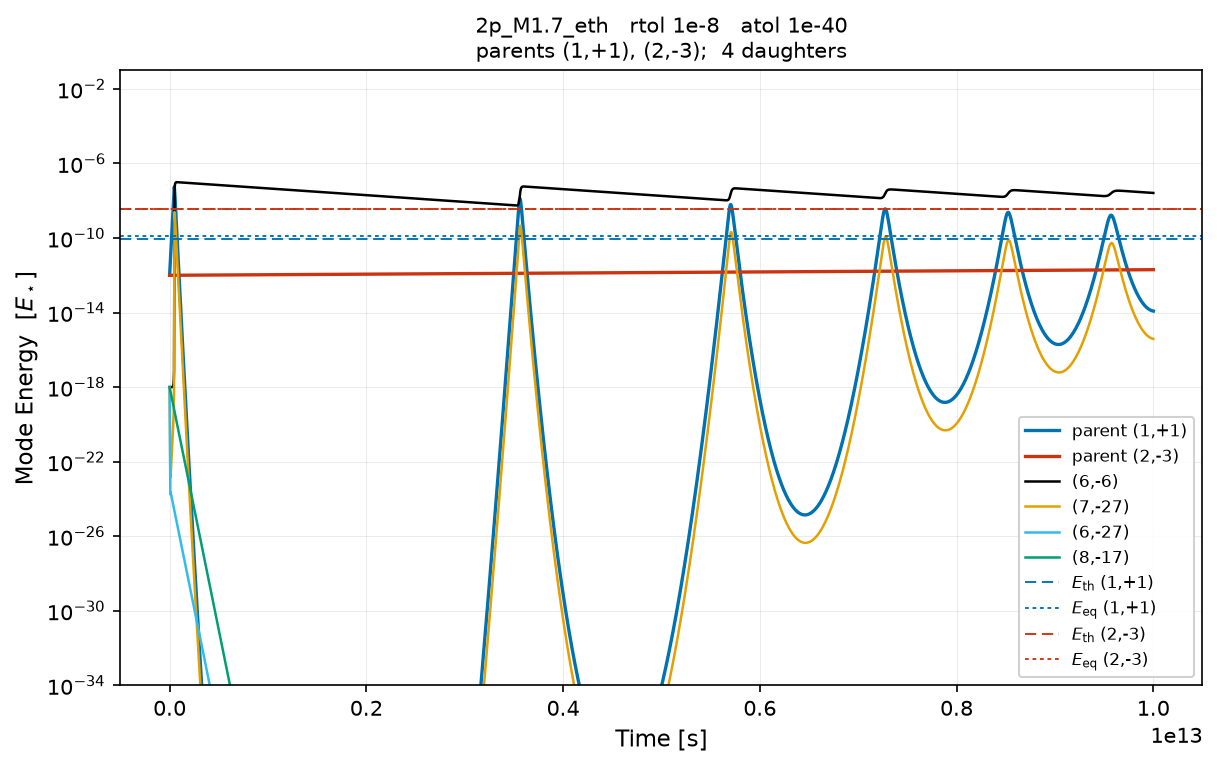
\includegraphics[width=0.21\textwidth,height=0.1323\textwidth]{../plots/rk8pd/2p_M1.7_eth/r1e-8_a1e-40.png} & 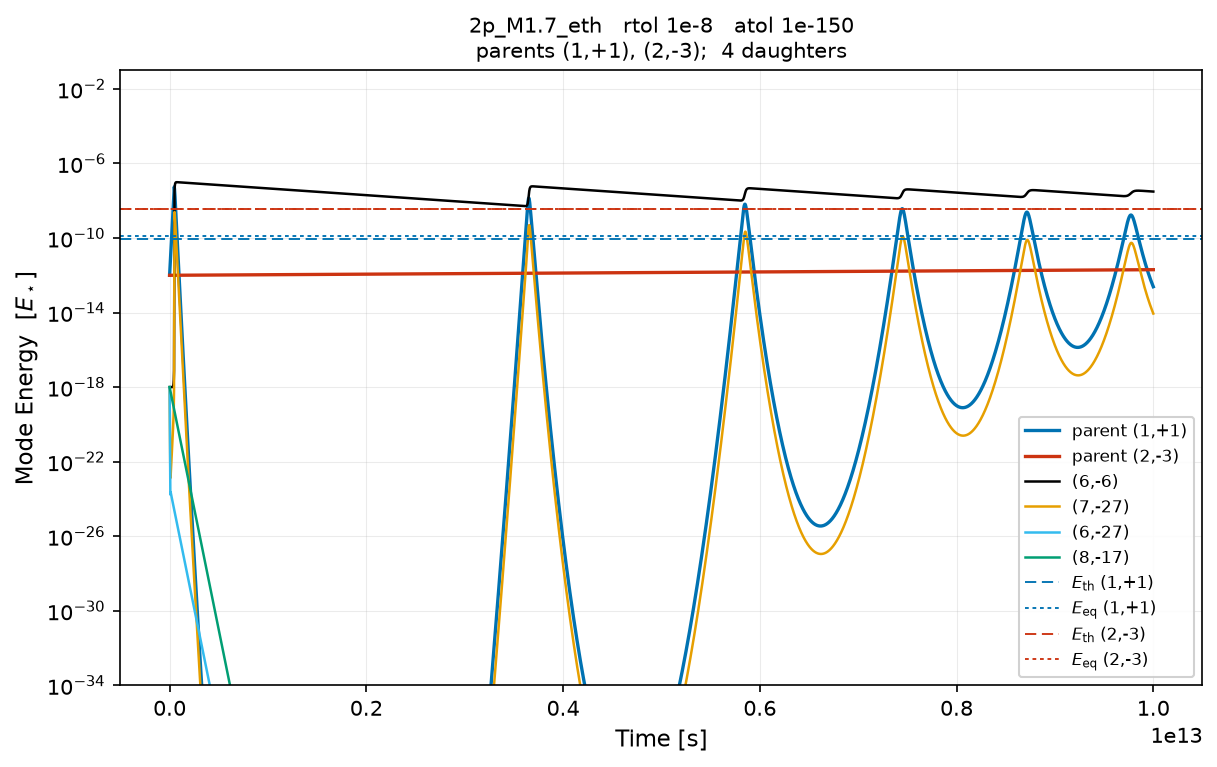
\includegraphics[width=0.21\textwidth,height=0.1323\textwidth]{../plots/rk8pd/2p_M1.7_eth/r1e-8_a1e-150.png} & 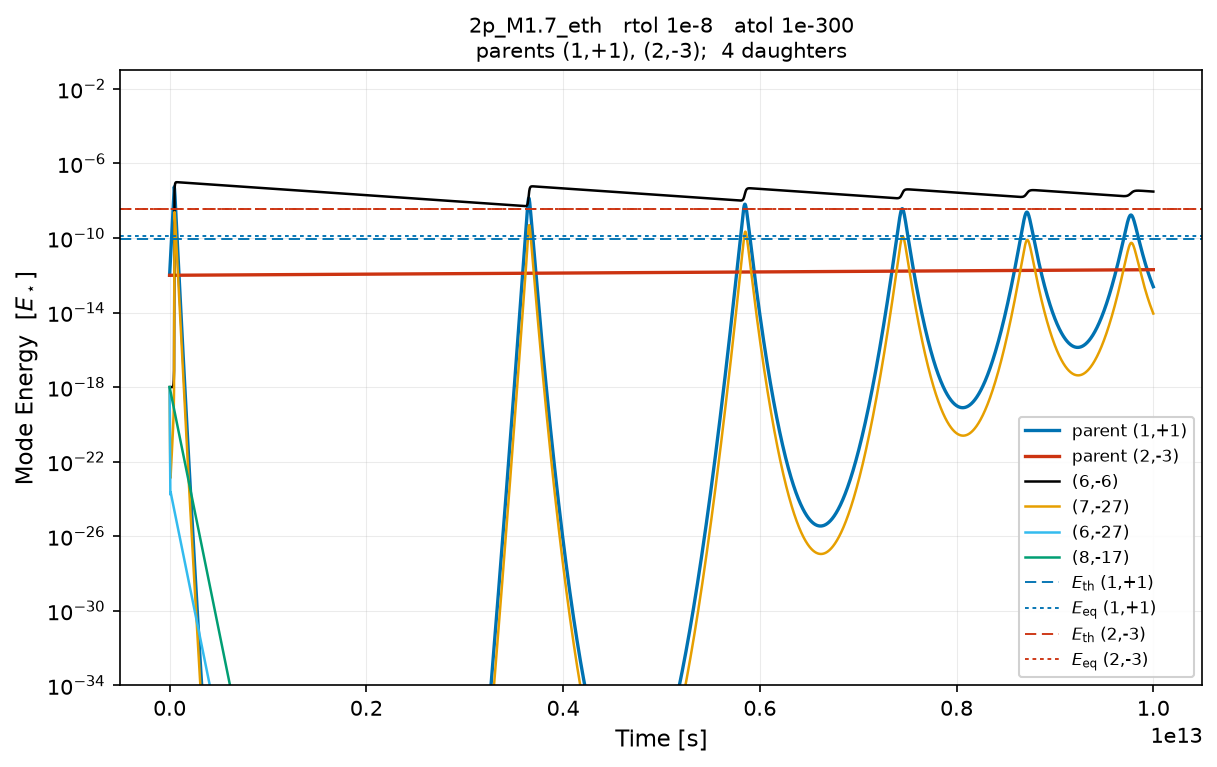
\includegraphics[width=0.21\textwidth,height=0.1323\textwidth]{../plots/rk8pd/2p_M1.7_eth/r1e-8_a1e-300.png} & 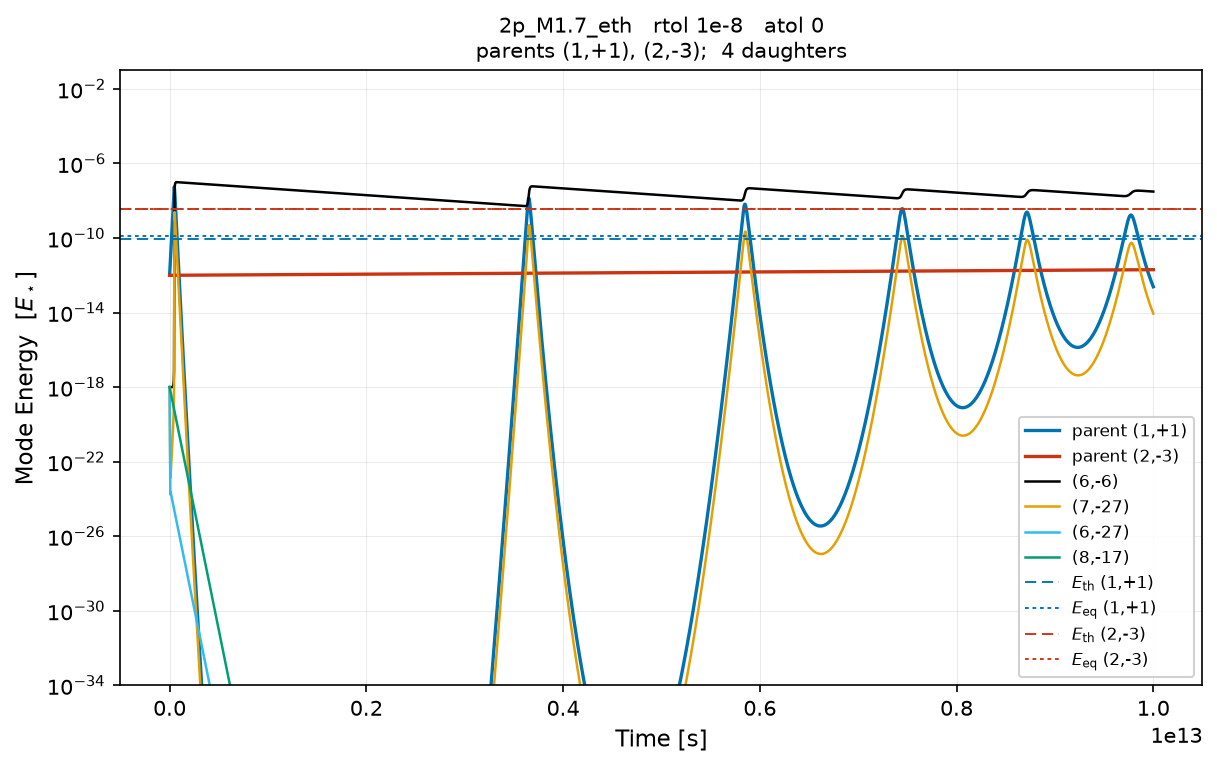
\includegraphics[width=0.21\textwidth,height=0.1323\textwidth]{../plots/rk8pd/2p_M1.7_eth/r1e-8_a0.png} \\[-1pt]
 & \parbox[t]{0.21\textwidth}{\centering\scriptsize 990.0\,k steps, 1.9\,s} & \parbox[t]{0.21\textwidth}{\centering\scriptsize 1.13\,M steps, 5.3\,s} & \parbox[t]{0.21\textwidth}{\centering\scriptsize 1.13\,M steps, 3.3\,s} & \parbox[t]{0.21\textwidth}{\centering\scriptsize 1.13\,M steps, 5.3\,s} \\[2pt]
\rotatebox{90}{\parbox{0.1323\textwidth}{\centering\scriptsize\bfseries BDF, dense analytic Jacobian}} & 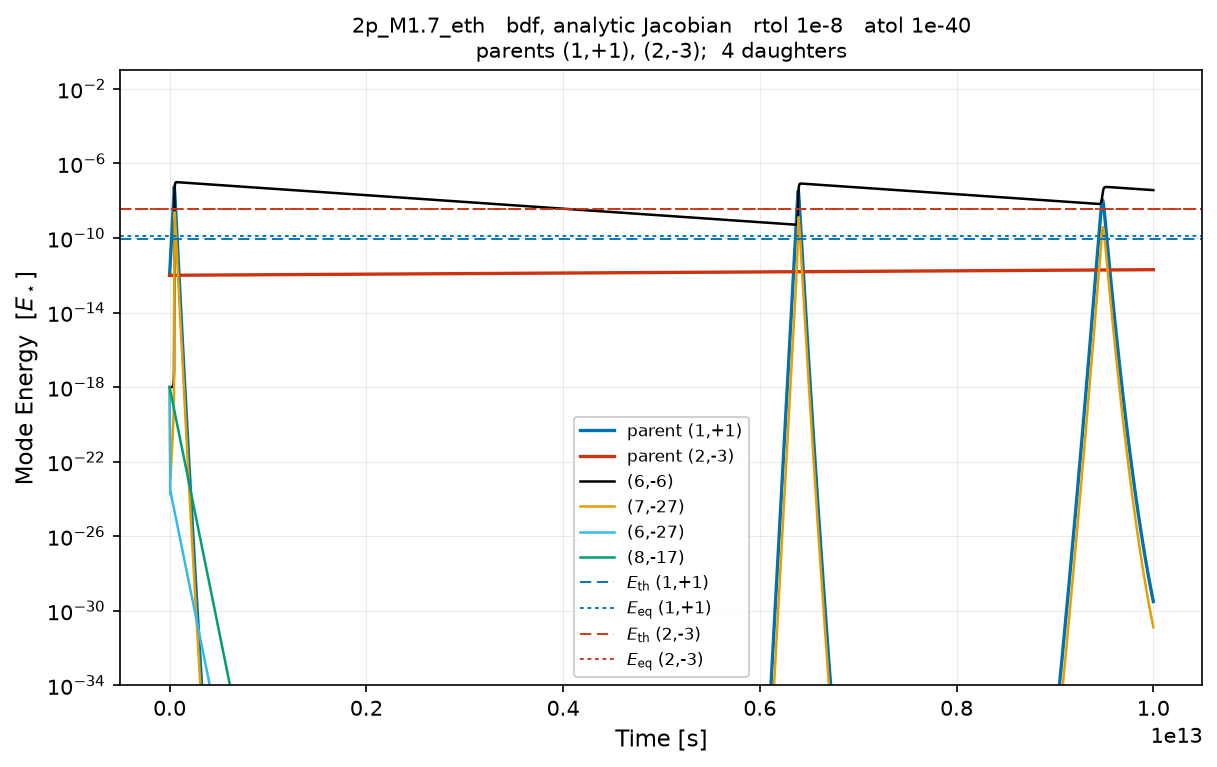
\includegraphics[width=0.21\textwidth,height=0.1323\textwidth]{../plots/bdf/2p_M1.7_eth/r1e-8_a1e-40.png} & 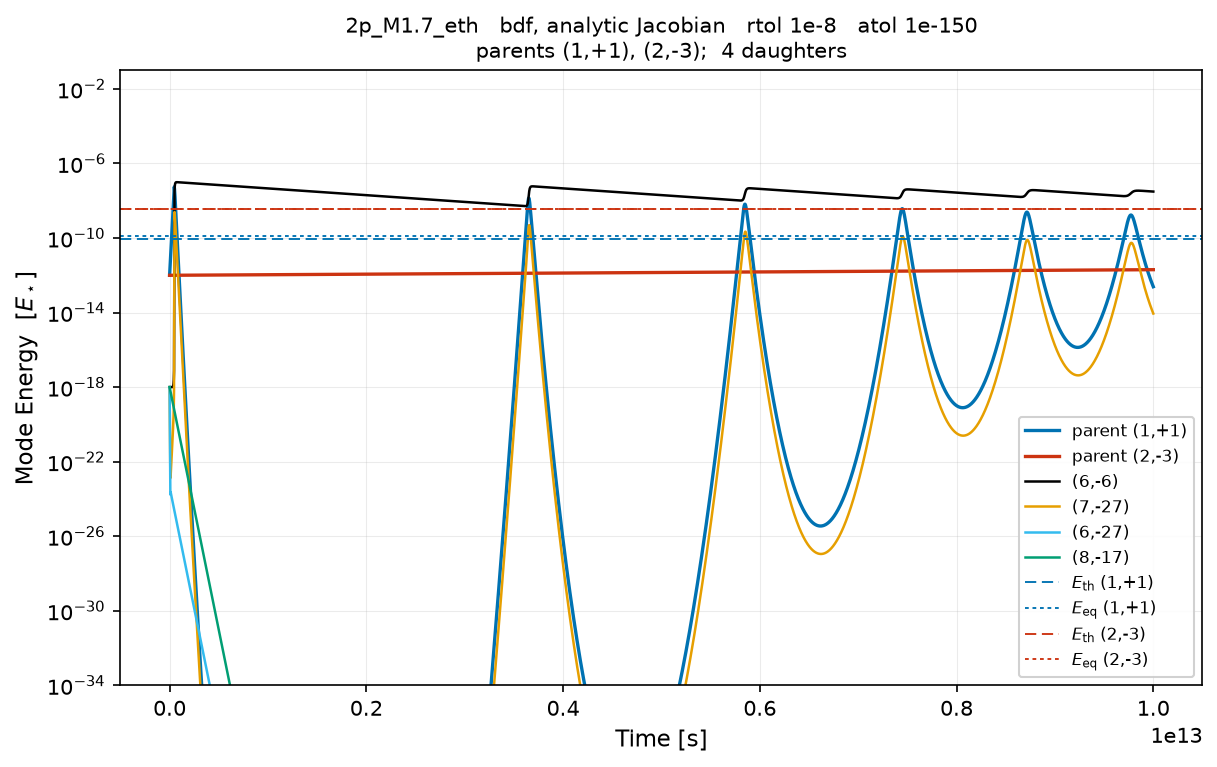
\includegraphics[width=0.21\textwidth,height=0.1323\textwidth]{../plots/bdf/2p_M1.7_eth/r1e-8_a1e-150.png} & 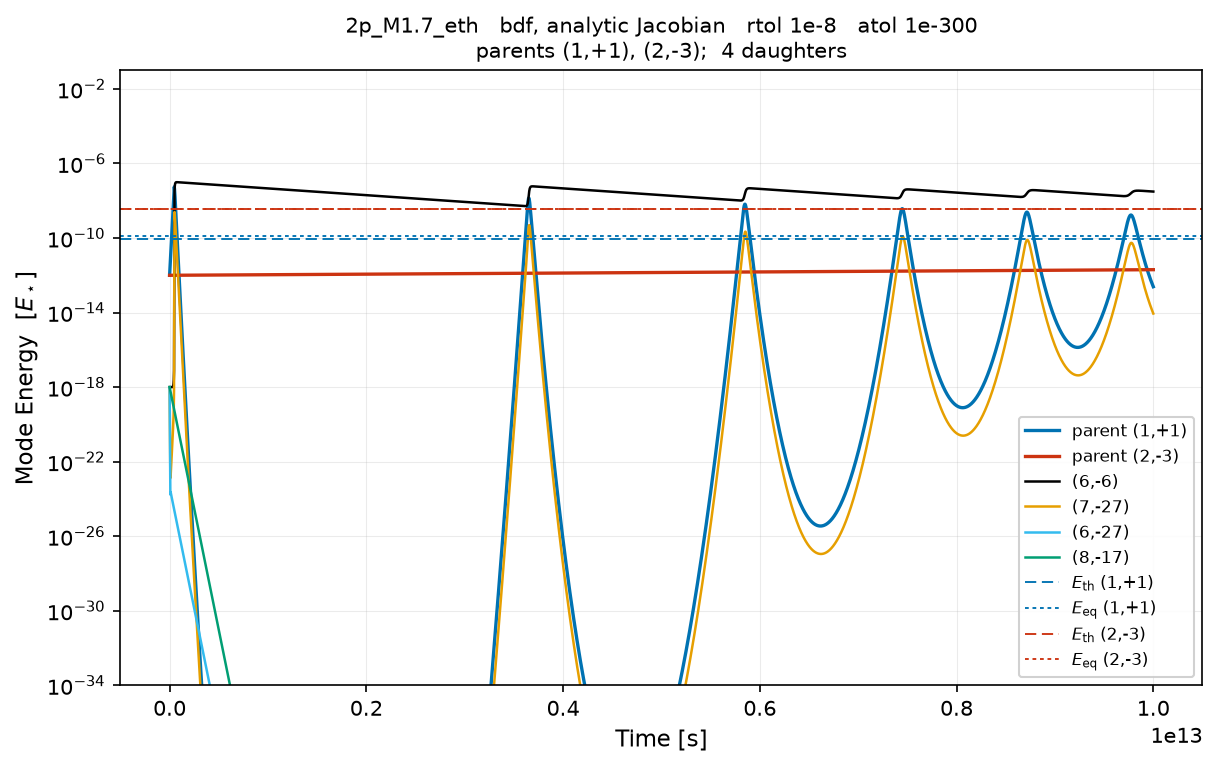
\includegraphics[width=0.21\textwidth,height=0.1323\textwidth]{../plots/bdf/2p_M1.7_eth/r1e-8_a1e-300.png} & 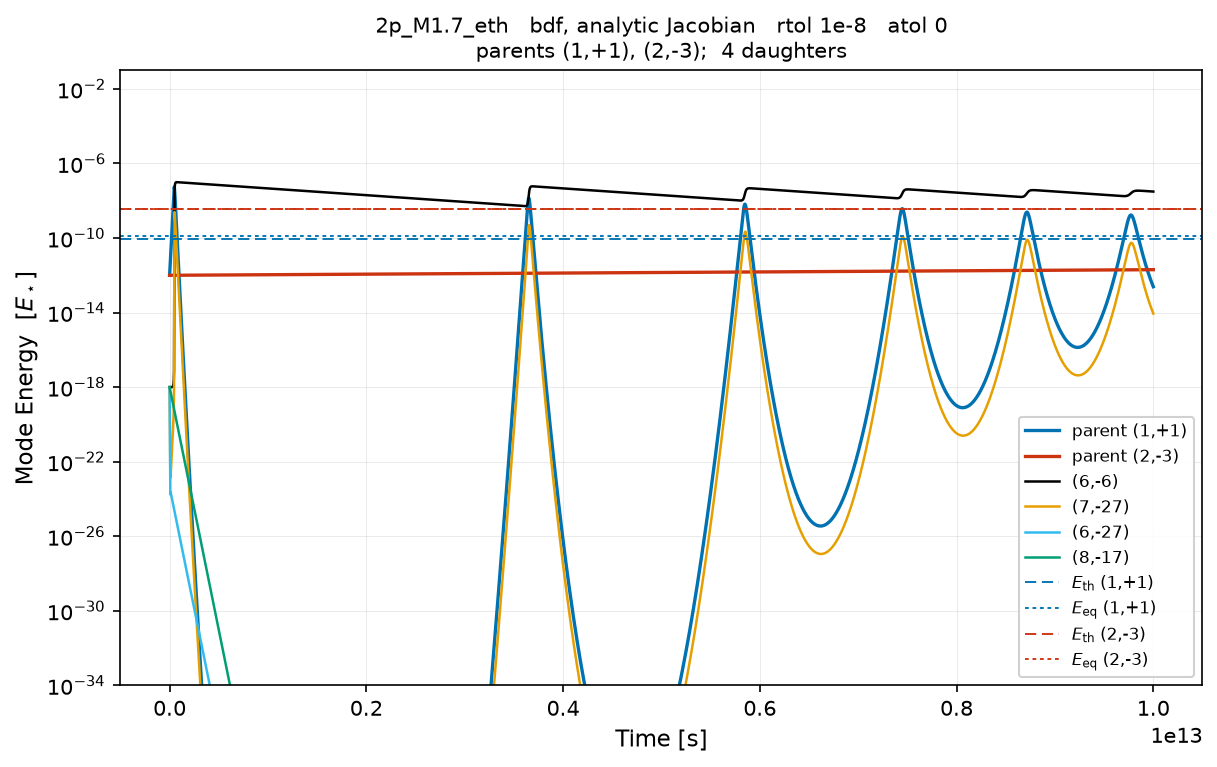
\includegraphics[width=0.21\textwidth,height=0.1323\textwidth]{../plots/bdf/2p_M1.7_eth/r1e-8_a0.png} \\[-1pt]
 & \parbox[t]{0.21\textwidth}{\centering\scriptsize 6.79\,M steps, 8.6\,s} & \parbox[t]{0.21\textwidth}{\centering\scriptsize 13.11\,M steps, 24.6\,s} & \parbox[t]{0.21\textwidth}{\centering\scriptsize 13.10\,M steps, 18.9\,s} & \parbox[t]{0.21\textwidth}{\centering\scriptsize 13.10\,M steps, 21.0\,s} \\[2pt]
\rotatebox{90}{\parbox{0.1323\textwidth}{\centering\scriptsize\bfseries BDF-Krylov, band full}} & 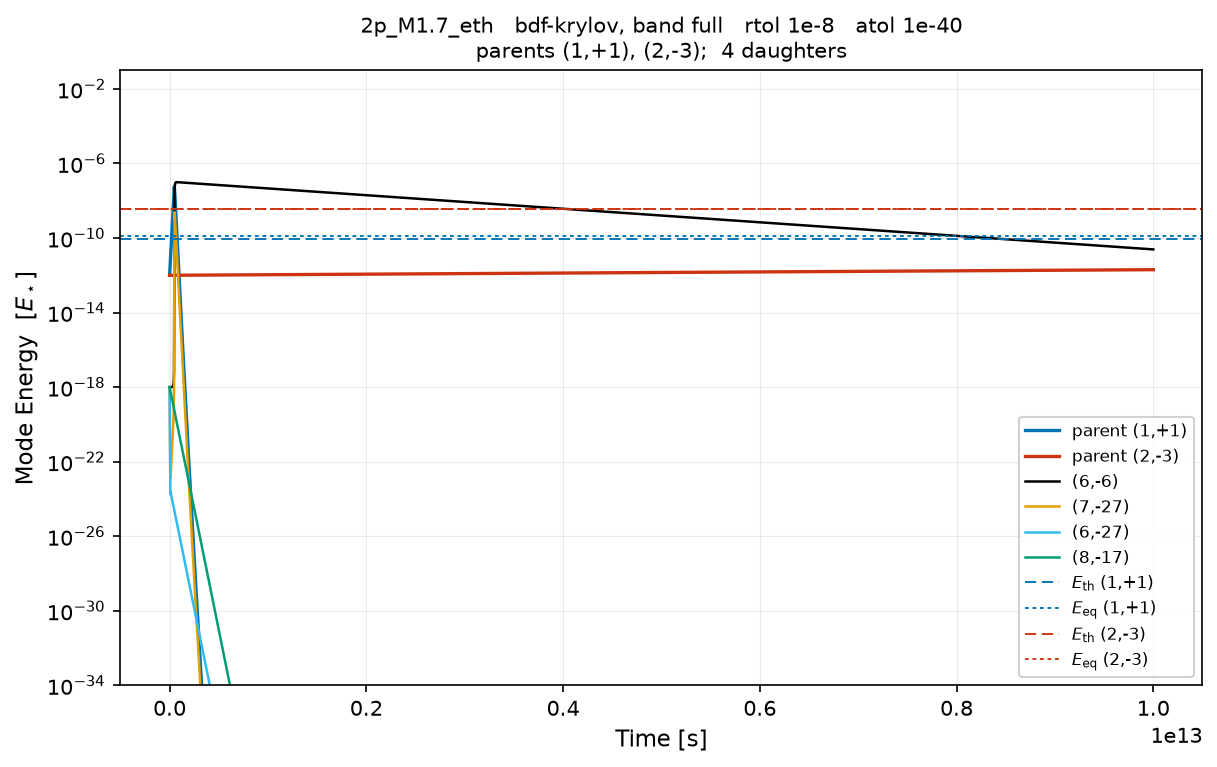
\includegraphics[width=0.21\textwidth,height=0.1323\textwidth]{../plots/krylov_full/2p_M1.7_eth/r1e-8_a1e-40.png} & 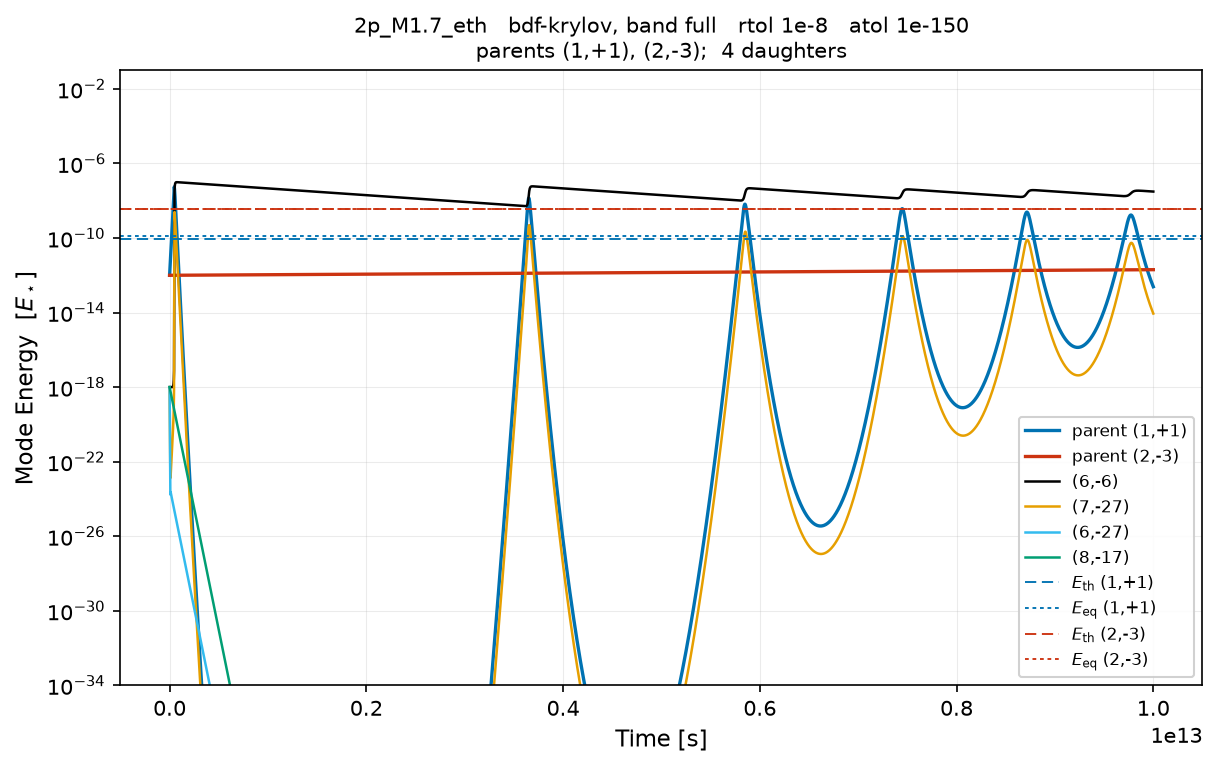
\includegraphics[width=0.21\textwidth,height=0.1323\textwidth]{../plots/krylov_full/2p_M1.7_eth/r1e-8_a1e-150.png} & 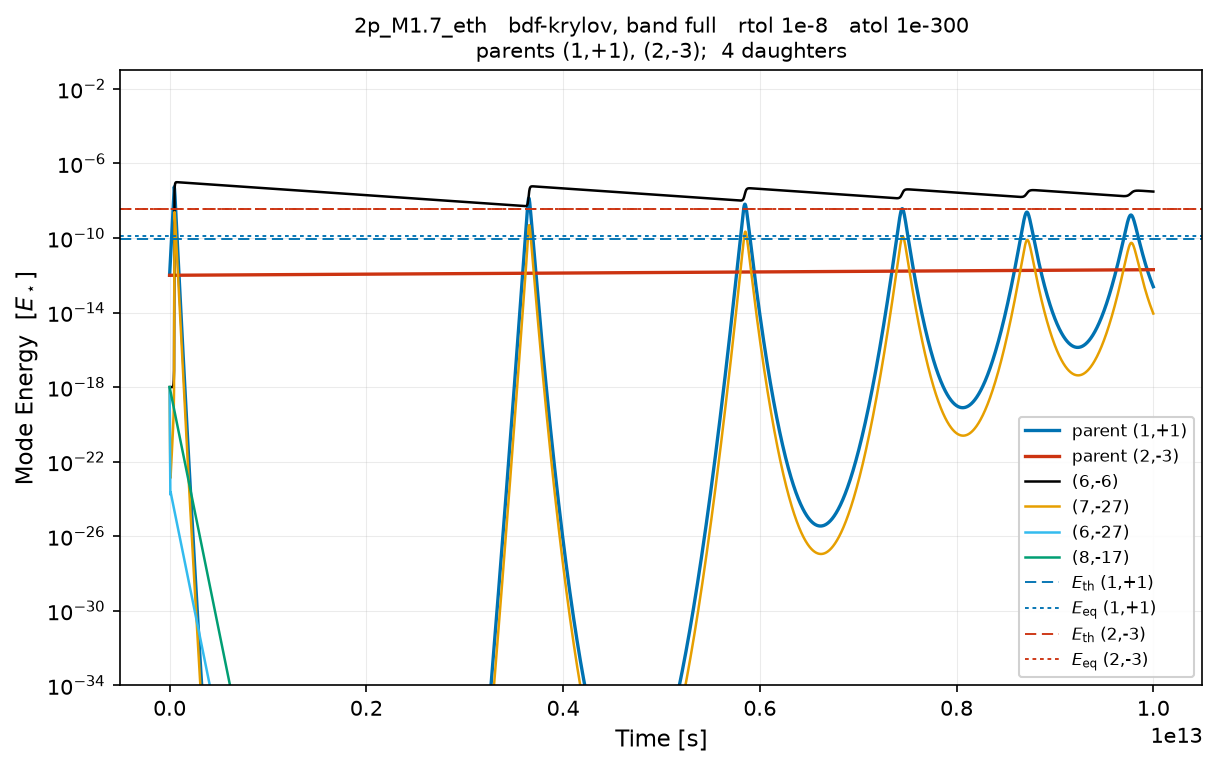
\includegraphics[width=0.21\textwidth,height=0.1323\textwidth]{../plots/krylov_full/2p_M1.7_eth/r1e-8_a1e-300.png} & 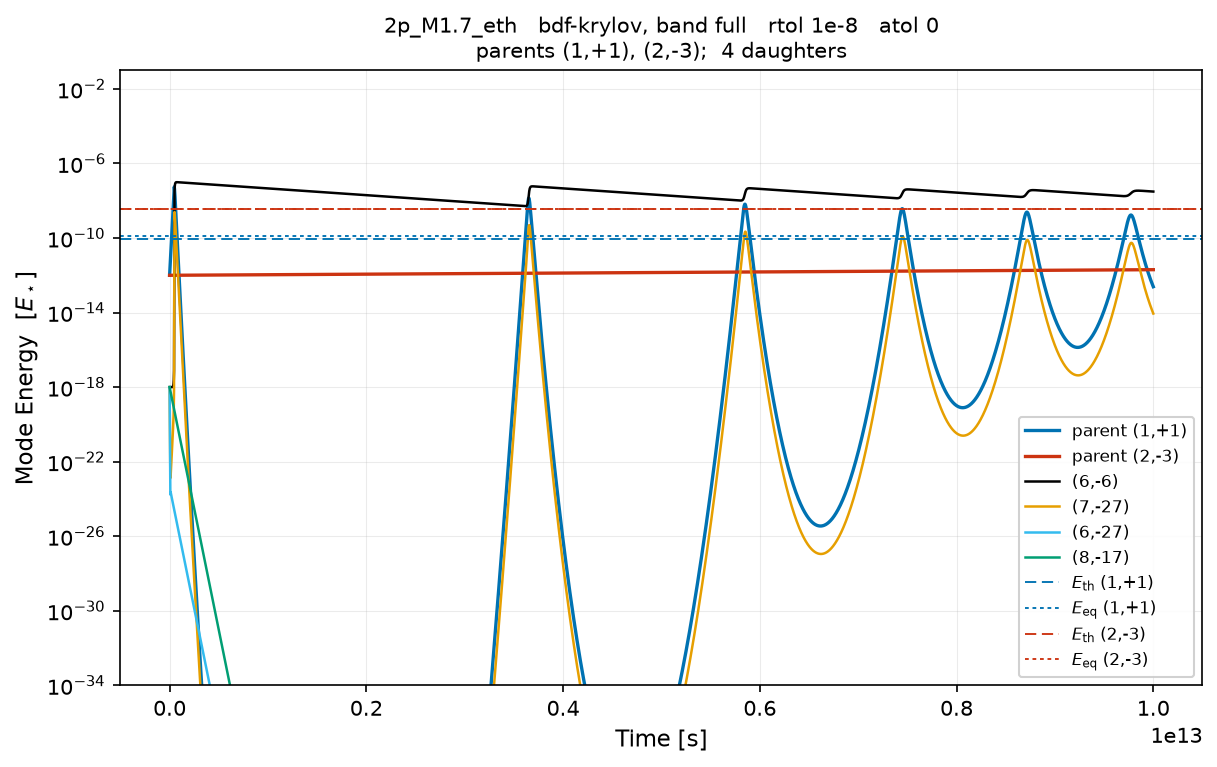
\includegraphics[width=0.21\textwidth,height=0.1323\textwidth]{../plots/krylov_full/2p_M1.7_eth/r1e-8_a0.png} \\[-1pt]
 & \parbox[t]{0.21\textwidth}{\centering\scriptsize 1.98\,M steps, 3.2\,s} & \parbox[t]{0.21\textwidth}{\centering\scriptsize 12.77\,M steps, 33.2\,s} & \parbox[t]{0.21\textwidth}{\centering\scriptsize 12.78\,M steps, 19.5\,s} & \parbox[t]{0.21\textwidth}{\centering\scriptsize 12.78\,M steps, 37.6\,s} \\[2pt]
\rotatebox{90}{\parbox{0.1323\textwidth}{\centering\scriptsize\bfseries BDF-Krylov, band 3}} & 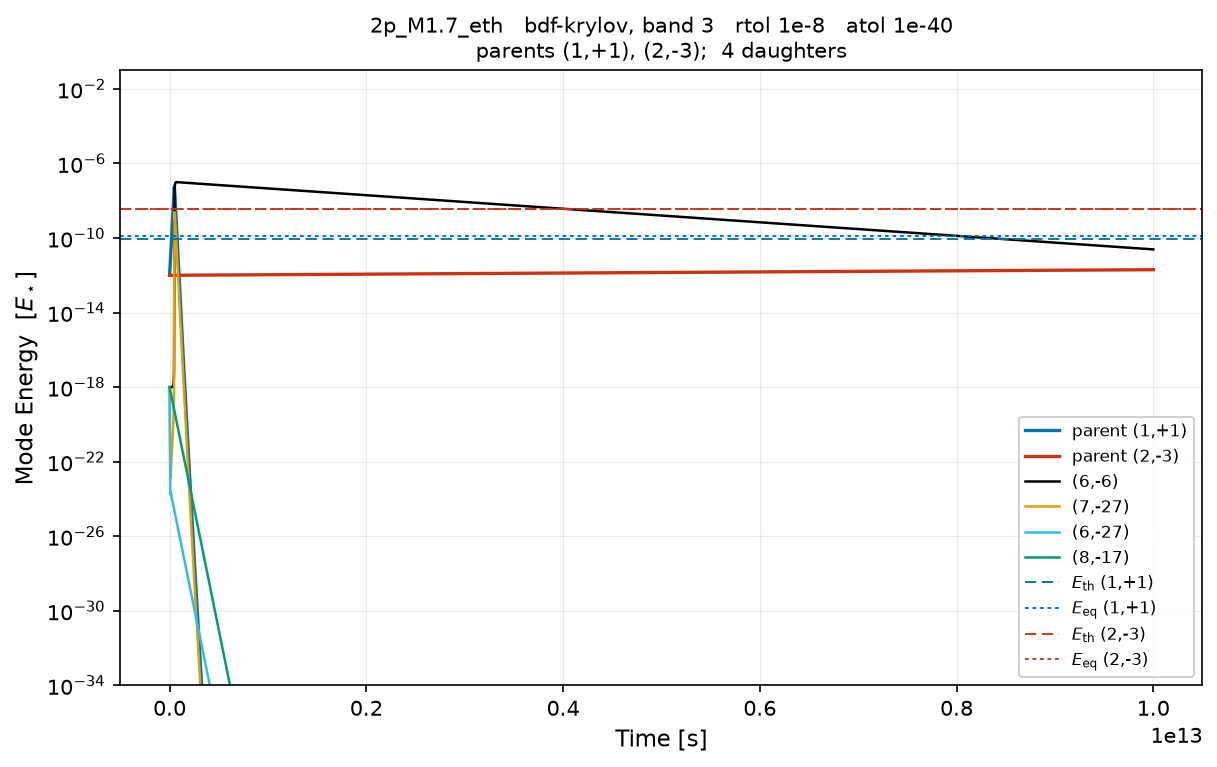
\includegraphics[width=0.21\textwidth,height=0.1323\textwidth]{../plots/krylov_b3/2p_M1.7_eth/r1e-8_a1e-40.png} & 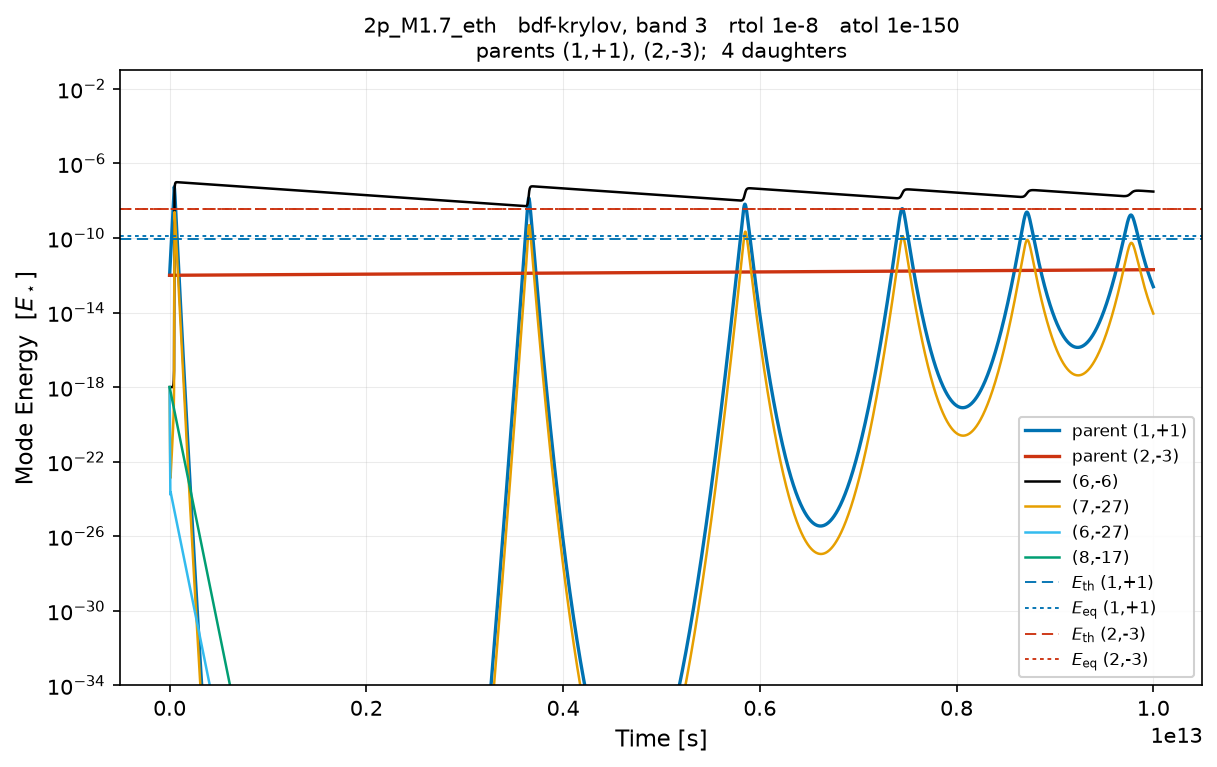
\includegraphics[width=0.21\textwidth,height=0.1323\textwidth]{../plots/krylov_b3/2p_M1.7_eth/r1e-8_a1e-150.png} & 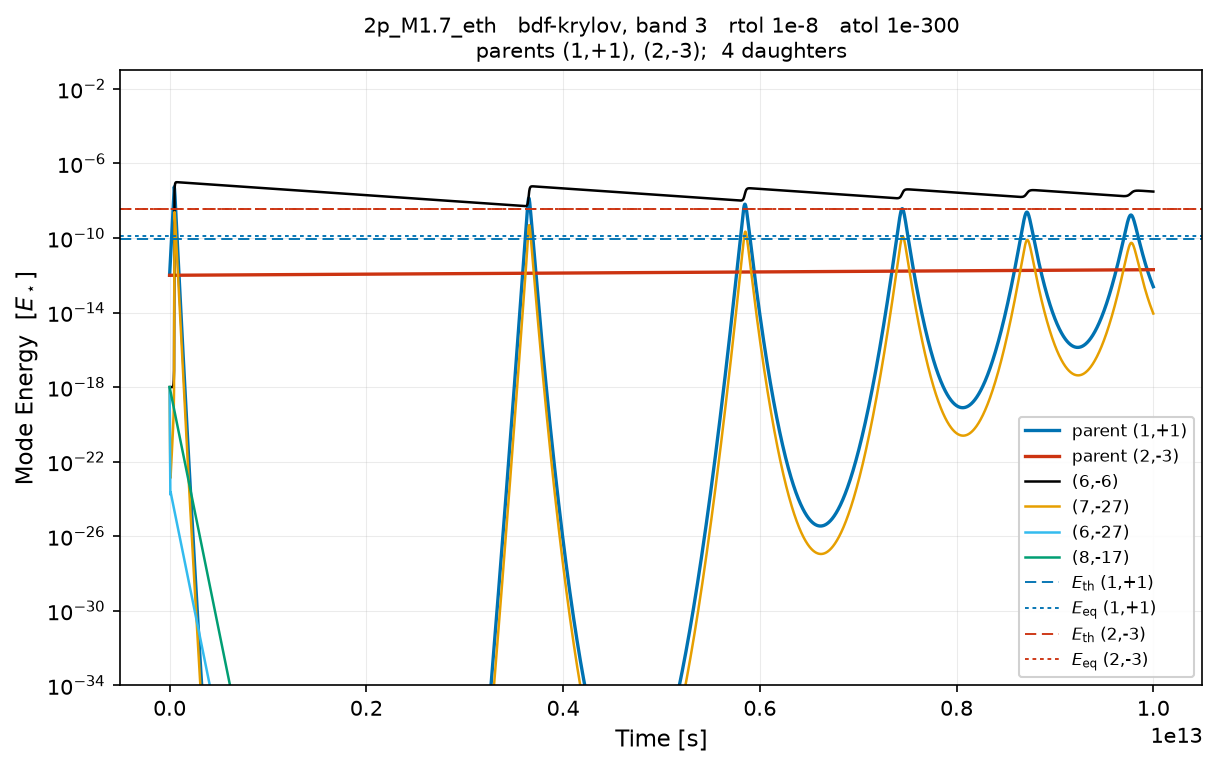
\includegraphics[width=0.21\textwidth,height=0.1323\textwidth]{../plots/krylov_b3/2p_M1.7_eth/r1e-8_a1e-300.png} & 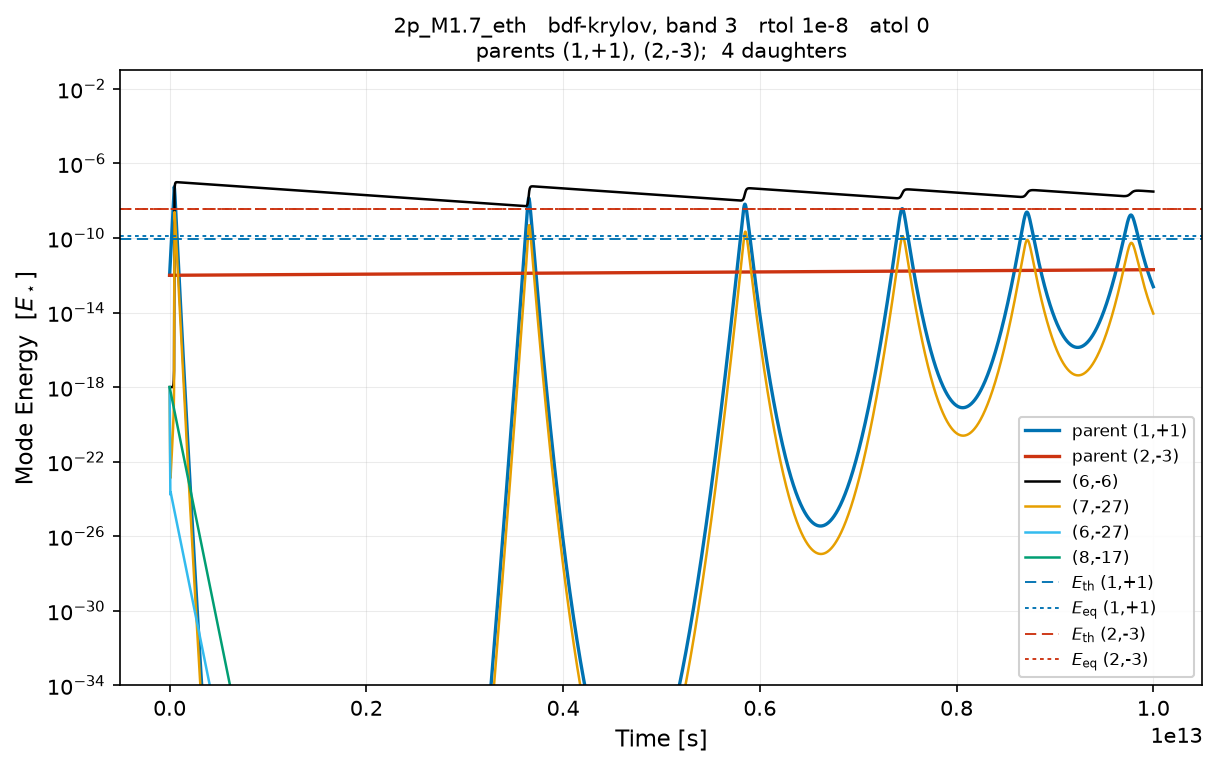
\includegraphics[width=0.21\textwidth,height=0.1323\textwidth]{../plots/krylov_b3/2p_M1.7_eth/r1e-8_a0.png} \\[-1pt]
 & \parbox[t]{0.21\textwidth}{\centering\scriptsize 2.19\,M steps, 6.3\,s} & \parbox[t]{0.21\textwidth}{\centering\scriptsize 12.40\,M steps, 38.2\,s} & \parbox[t]{0.21\textwidth}{\centering\scriptsize 12.41\,M steps, 27.7\,s} & \parbox[t]{0.21\textwidth}{\centering\scriptsize 12.41\,M steps, 24.7\,s} \\[2pt]
\rotatebox{90}{\parbox{0.1323\textwidth}{\centering\scriptsize\bfseries Adams, fixed point}} & 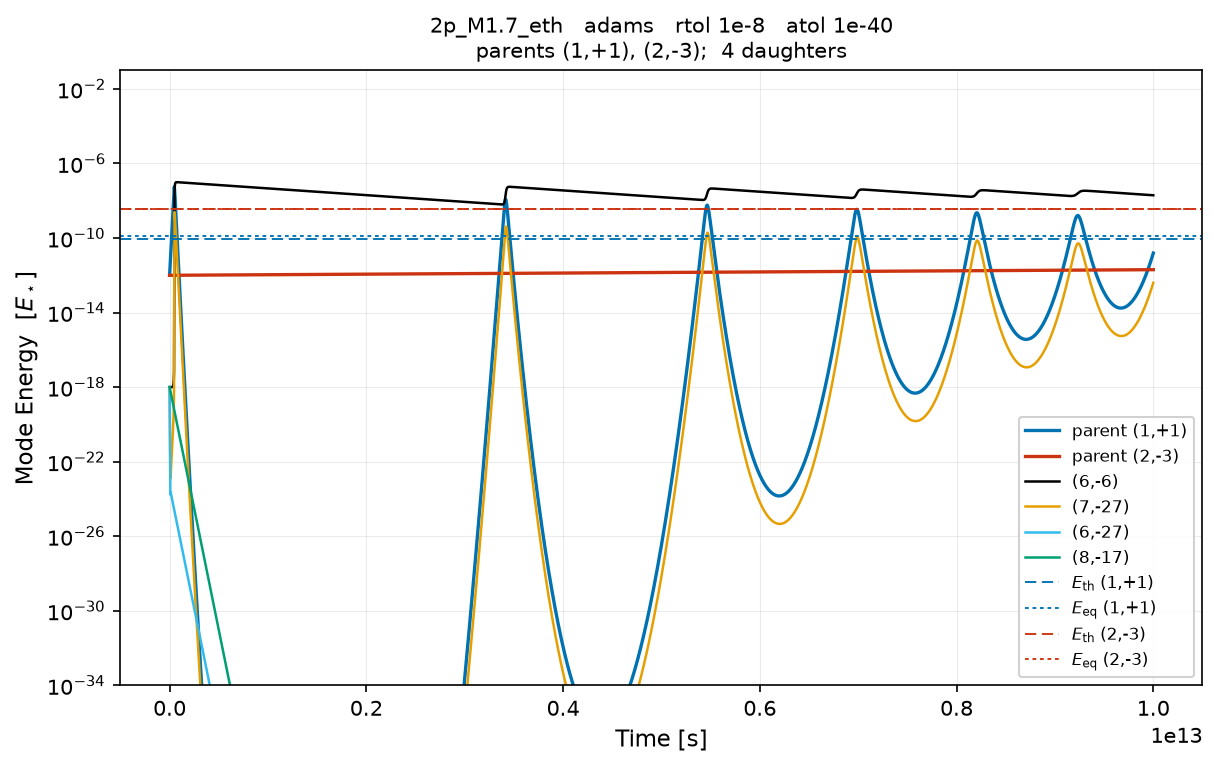
\includegraphics[width=0.21\textwidth,height=0.1323\textwidth]{../plots/adams/2p_M1.7_eth/r1e-8_a1e-40.png} & 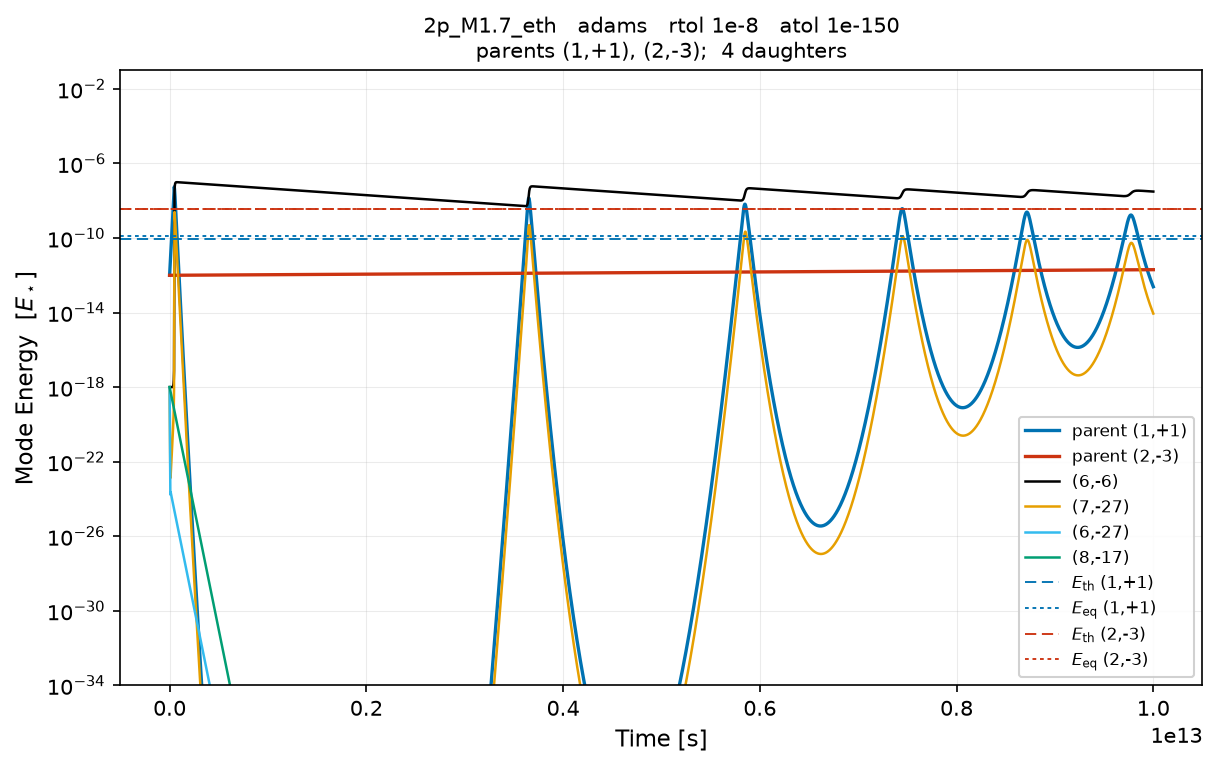
\includegraphics[width=0.21\textwidth,height=0.1323\textwidth]{../plots/adams/2p_M1.7_eth/r1e-8_a1e-150.png} & 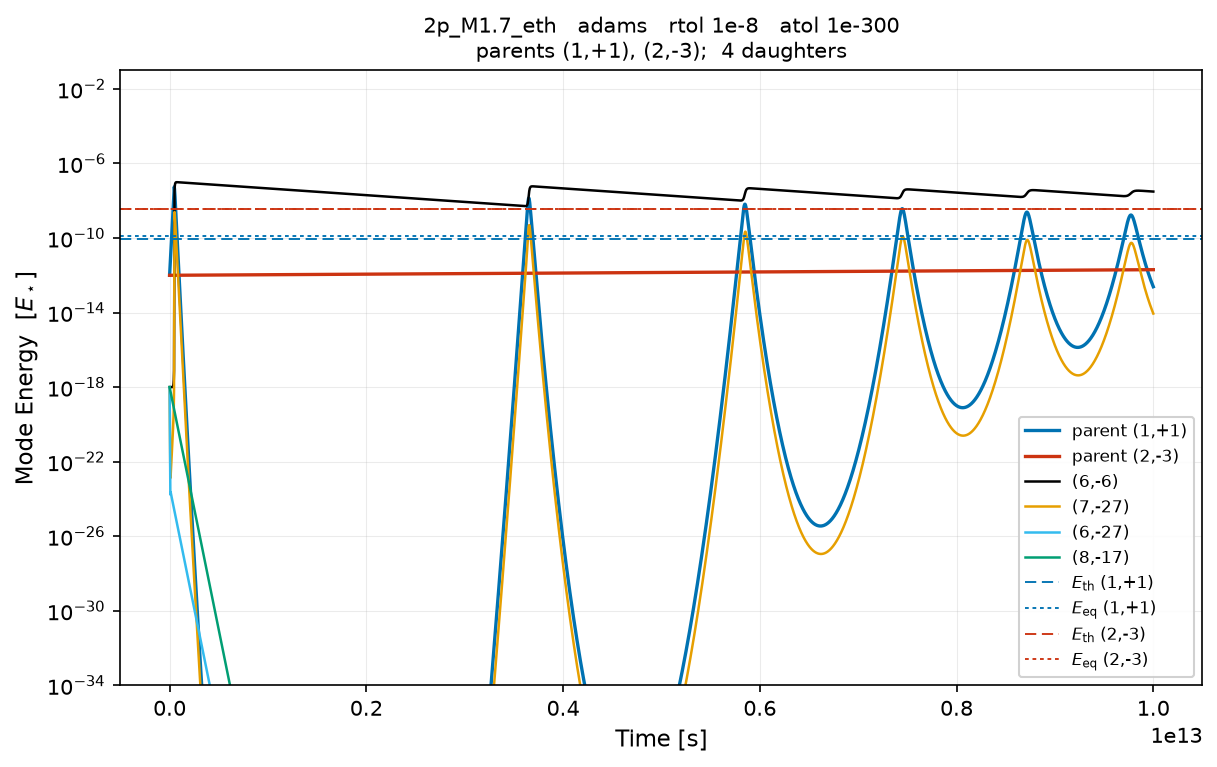
\includegraphics[width=0.21\textwidth,height=0.1323\textwidth]{../plots/adams/2p_M1.7_eth/r1e-8_a1e-300.png} & 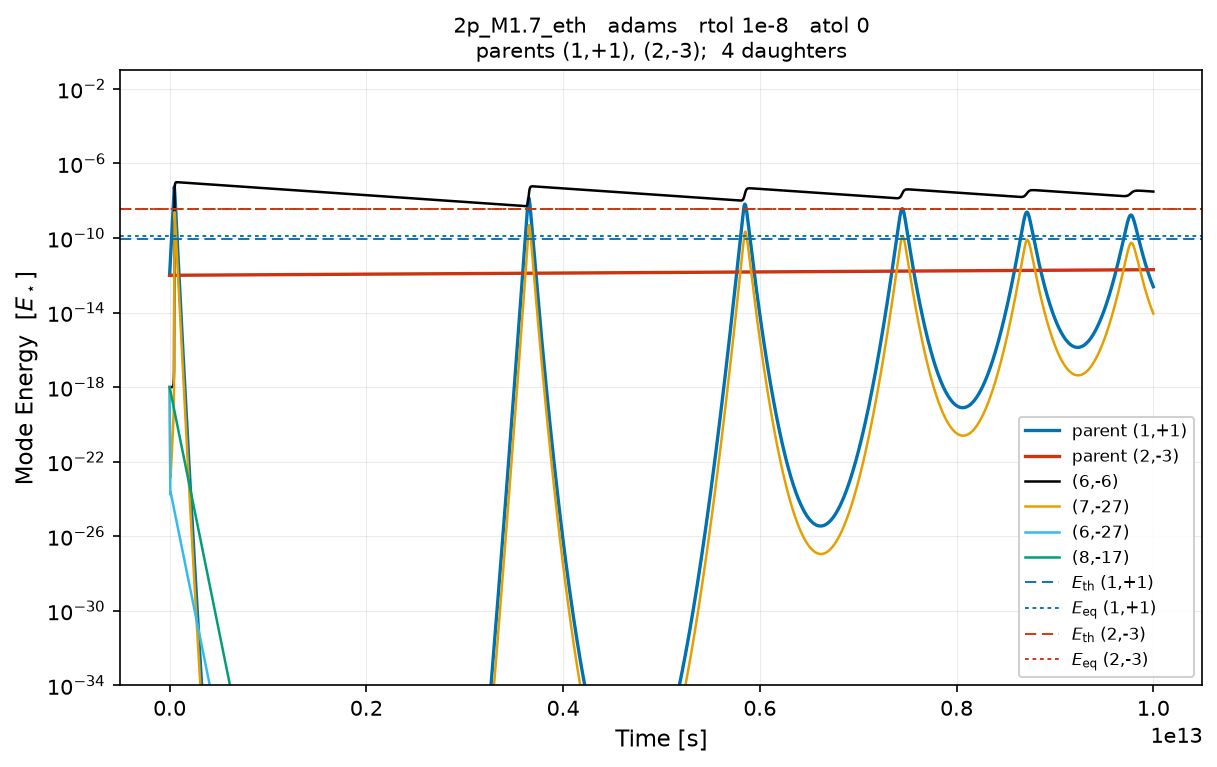
\includegraphics[width=0.21\textwidth,height=0.1323\textwidth]{../plots/adams/2p_M1.7_eth/r1e-8_a0.png} \\[-1pt]
 & \parbox[t]{0.21\textwidth}{\centering\scriptsize 5.42\,M steps, 9.2\,s} & \parbox[t]{0.21\textwidth}{\centering\scriptsize 5.69\,M steps, 9.5\,s} & \parbox[t]{0.21\textwidth}{\centering\scriptsize 5.69\,M steps, 5.6\,s} & \parbox[t]{0.21\textwidth}{\centering\scriptsize 5.69\,M steps, 6.3\,s} \\[2pt]
\end{tabular}\par}
\par\noindent{\scriptsize\setlength\tabcolsep{3.5pt}\renewcommand\arraystretch{0.92}
\begin{tabular}{@{}llllrrrrrrr@{}}
\toprule
integrator & atol & stop & $t_{\rm stop}$ [s] & steps & rejected & RHS & Jac. & NL it. & lin. it. & wall [s] \\
\midrule
rk8pd & $10^{-40}$ & end & $1.00\times10^{13}$ & 990.0\,k & 104.5\,k & 12.87\,M & -- & -- & -- & 1.9 \\
 & $10^{-150}$ & end & $1.00\times10^{13}$ & 1.13\,M & 128.5\,k & 14.69\,M & -- & -- & -- & 5.3 \\
 & $10^{-300}$ & end & $1.00\times10^{13}$ & 1.13\,M & 128.6\,k & 14.69\,M & -- & -- & -- & 3.3 \\
 & $0$ & end & $1.00\times10^{13}$ & 1.13\,M & 128.6\,k & 14.69\,M & -- & -- & -- & 5.3 \\
\addlinespace[2pt]
BDF, dense analytic Jacobian & $10^{-40}$ & end & $1.00\times10^{13}$ & 6.79\,M & 49.2\,k & 7.26\,M & 120.3\,k & 7.26\,M & -- & 8.6 \\
 & $10^{-150}$ & end & $1.00\times10^{13}$ & 13.11\,M & 133.6\,k & 14.11\,M & 230.1\,k & 14.11\,M & -- & 24.6 \\
 & $10^{-300}$ & end & $1.00\times10^{13}$ & 13.10\,M & 133.6\,k & 14.11\,M & 230.1\,k & 14.10\,M & -- & 18.9 \\
 & $0$ & end & $1.00\times10^{13}$ & 13.10\,M & 133.6\,k & 14.11\,M & 230.1\,k & 14.10\,M & -- & 21.0 \\
\addlinespace[2pt]
BDF-Krylov, band full & $10^{-40}$ & end & $1.00\times10^{13}$ & 1.98\,M & 16.0\,k & 4.65\,M & 37.6\,k & 2.12\,M & 2.08\,M & 3.2 \\
 & $10^{-150}$ & end & $1.00\times10^{13}$ & 12.77\,M & 148.3\,k & 29.89\,M & 223.9\,k & 13.86\,M & 13.34\,M & 33.2 \\
 & $10^{-300}$ & end & $1.00\times10^{13}$ & 12.78\,M & 147.9\,k & 29.90\,M & 224.0\,k & 13.86\,M & 13.34\,M & 19.5 \\
 & $0$ & end & $1.00\times10^{13}$ & 12.78\,M & 147.9\,k & 29.90\,M & 224.0\,k & 13.86\,M & 13.34\,M & 37.6 \\
\addlinespace[2pt]
BDF-Krylov, band 3 & $10^{-40}$ & end & $1.00\times10^{13}$ & 2.19\,M & 24.0\,k & 5.58\,M & 41.3\,k & 2.39\,M & 2.90\,M & 6.3 \\
 & $10^{-150}$ & end & $1.00\times10^{13}$ & 12.40\,M & 183.1\,k & 31.21\,M & 217.9\,k & 13.67\,M & 16.01\,M & 38.2 \\
 & $10^{-300}$ & end & $1.00\times10^{13}$ & 12.41\,M & 183.7\,k & 31.21\,M & 217.9\,k & 13.67\,M & 16.01\,M & 27.7 \\
 & $0$ & end & $1.00\times10^{13}$ & 12.41\,M & 183.7\,k & 31.21\,M & 217.9\,k & 13.67\,M & 16.01\,M & 24.7 \\
\addlinespace[2pt]
Adams, fixed point & $10^{-40}$ & end & $1.00\times10^{13}$ & 5.42\,M & 223.9\,k & 8.29\,M & -- & 8.29\,M & -- & 9.2 \\
 & $10^{-150}$ & end & $1.00\times10^{13}$ & 5.69\,M & 277.3\,k & 8.45\,M & -- & 8.44\,M & -- & 9.5 \\
 & $10^{-300}$ & end & $1.00\times10^{13}$ & 5.69\,M & 277.7\,k & 8.43\,M & -- & 8.43\,M & -- & 5.6 \\
 & $0$ & end & $1.00\times10^{13}$ & 5.69\,M & 277.7\,k & 8.43\,M & -- & 8.43\,M & -- & 6.3 \\
\bottomrule
\end{tabular}}

\clearpage
\subsection{\texttt{2p\_M2.0T\_eth}}\label{net:2p_M2.0T_eth}
\noindent\begin{minipage}[t]{0.43\textwidth}\vspace{0pt}\footnotesize
\begin{tabular}{@{}rrlrr@{}}
\toprule
id & gen & $(\ell,n)$ & $\omega$ [rad\,s$^{-1}$] & $\gamma$ [s$^{-1}$] \\
\midrule
0 & 0 & (2,$-$3) & $6.816\times10^{-4}$ & $-8.642\times10^{-13}$ \\
1 & 0 & (2,$-$2) & $7.959\times10^{-4}$ & $-6.697\times10^{-11}$ \\
2 & 1 & (14,$-$48) & $3.408\times10^{-4}$ & $1.376\times10^{-9}$ \\
3 & 1 & (3,$-$31) & $1.287\times10^{-4}$ & $8.096\times10^{-11}$ \\
4 & 1 & (5,$-$8) & $6.672\times10^{-4}$ & $7.367\times10^{-13}$ \\
\bottomrule
\end{tabular}
\end{minipage}\hfill
\begin{minipage}[t]{0.55\textwidth}\vspace{0pt}\footnotesize
\textbf{Model} \texttt{dsct\_M2.0\_T7696}, rule eth, $N=1$, cut 0.15,
closure 0.005; 5 modes, 2 triplet(s).\\[2pt]
\textbf{Selecting pairs}\\ (2,$-$3) $\to$ (14,$-$48) + (14,$-$48): $\Delta/\omega_a=-6.00\times10^{-6}$, $\kappa=-0.452$, $E_{\rm th}=6.40\times10^{-11}$, $E_{\rm eq}=6.40\times10^{-11}$\\
(2,$-$2) $\to$ (3,$-$31) + (5,$-$8): $\Delta/\omega_a=-3.69\times10^{-6}$, $\kappa=+0.215$, $E_{\rm th}=4.87\times10^{-12}$, $E_{\rm eq}=1.50\times10^{-10}$\\[2pt]
Daughter (14,$-48$) decays to $E\sim10^{-3600}$ in exact arithmetic; its regrowth time is set by each run's floor.
\end{minipage}

\par\smallskip{\centering\begin{tabular}{@{}c@{\hspace{2pt}}c@{\hspace{2pt}}c@{\hspace{2pt}}c@{\hspace{2pt}}c@{}}
 & \small atol $10^{-40}$ & \small atol $10^{-150}$ & \small atol $10^{-300}$ & \small atol $0$ \\[1pt]
\rotatebox{90}{\parbox{0.1323\textwidth}{\centering\scriptsize\bfseries rk8pd}} & 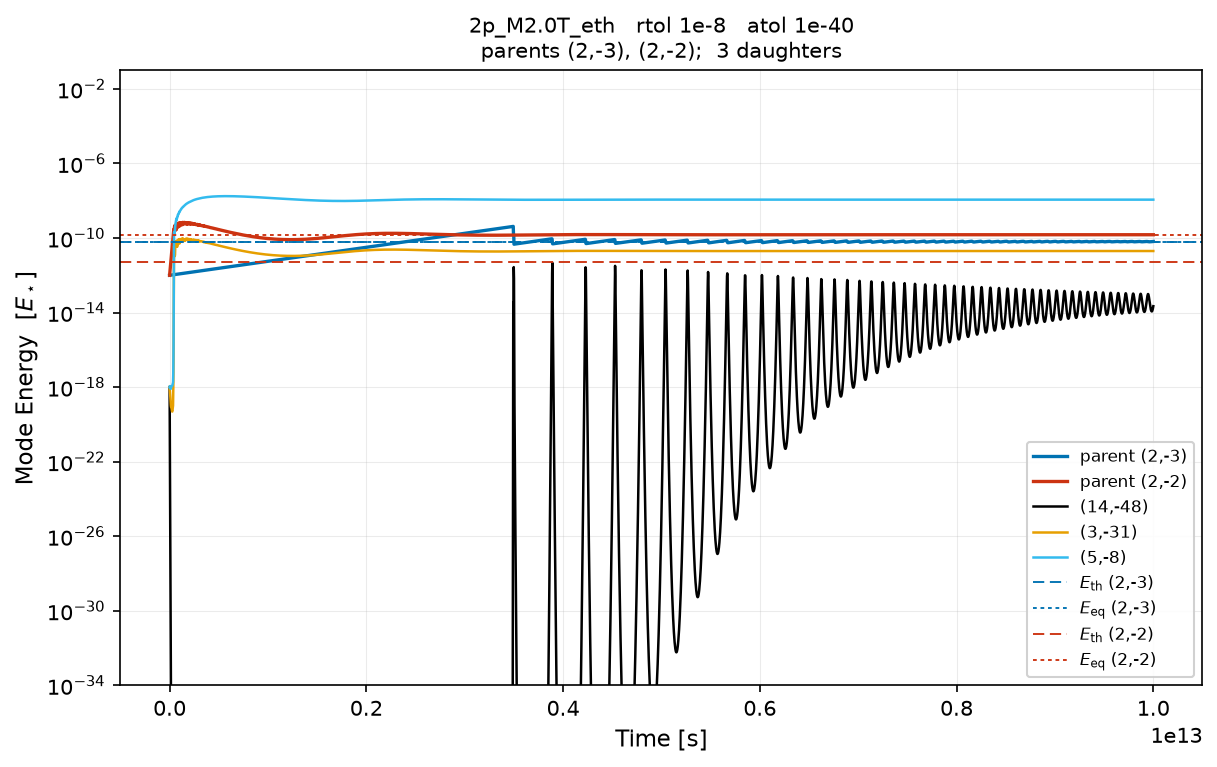
\includegraphics[width=0.21\textwidth,height=0.1323\textwidth]{../plots/rk8pd/2p_M2.0T_eth/r1e-8_a1e-40.png} & 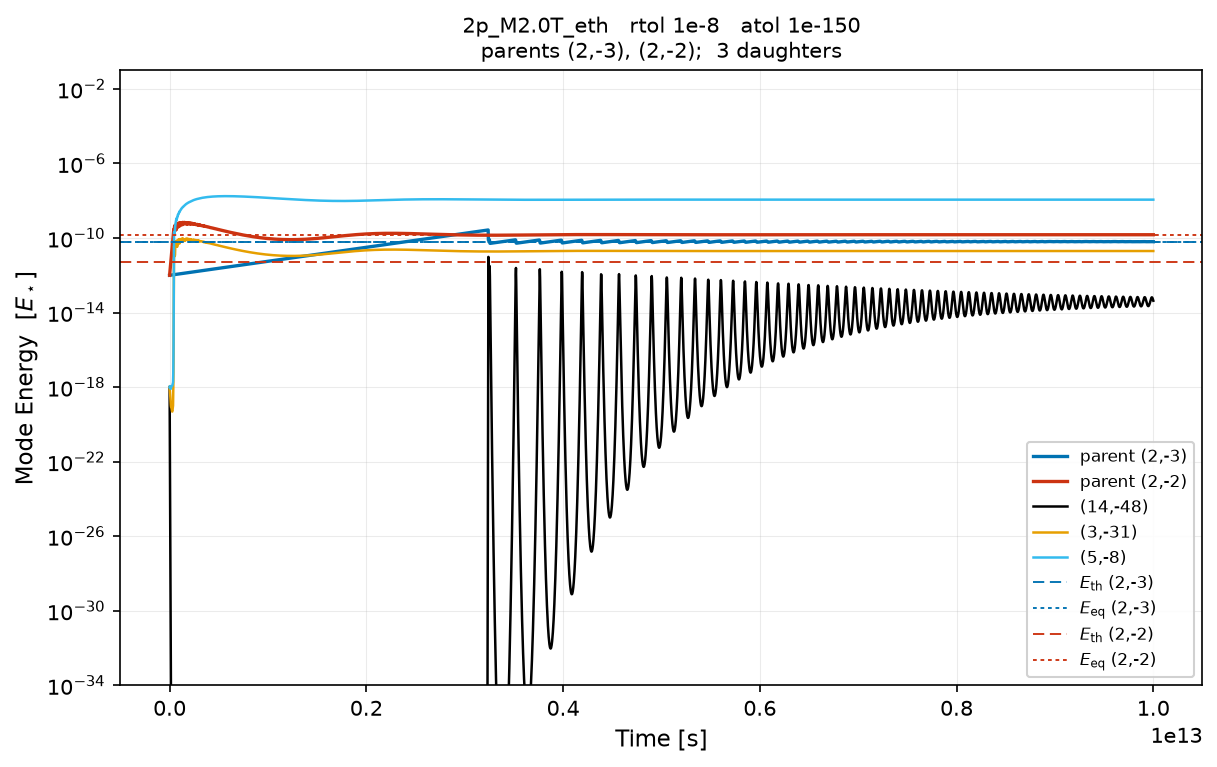
\includegraphics[width=0.21\textwidth,height=0.1323\textwidth]{../plots/rk8pd/2p_M2.0T_eth/r1e-8_a1e-150.png} & 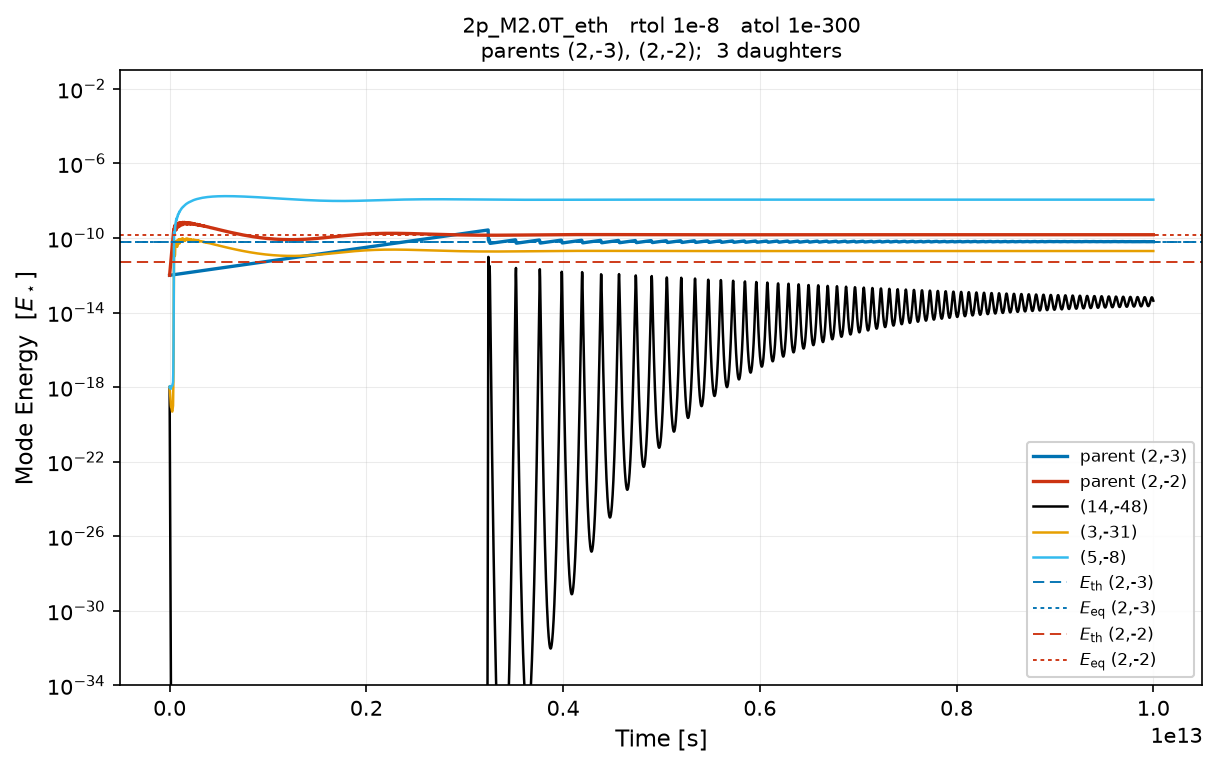
\includegraphics[width=0.21\textwidth,height=0.1323\textwidth]{../plots/rk8pd/2p_M2.0T_eth/r1e-8_a1e-300.png} & 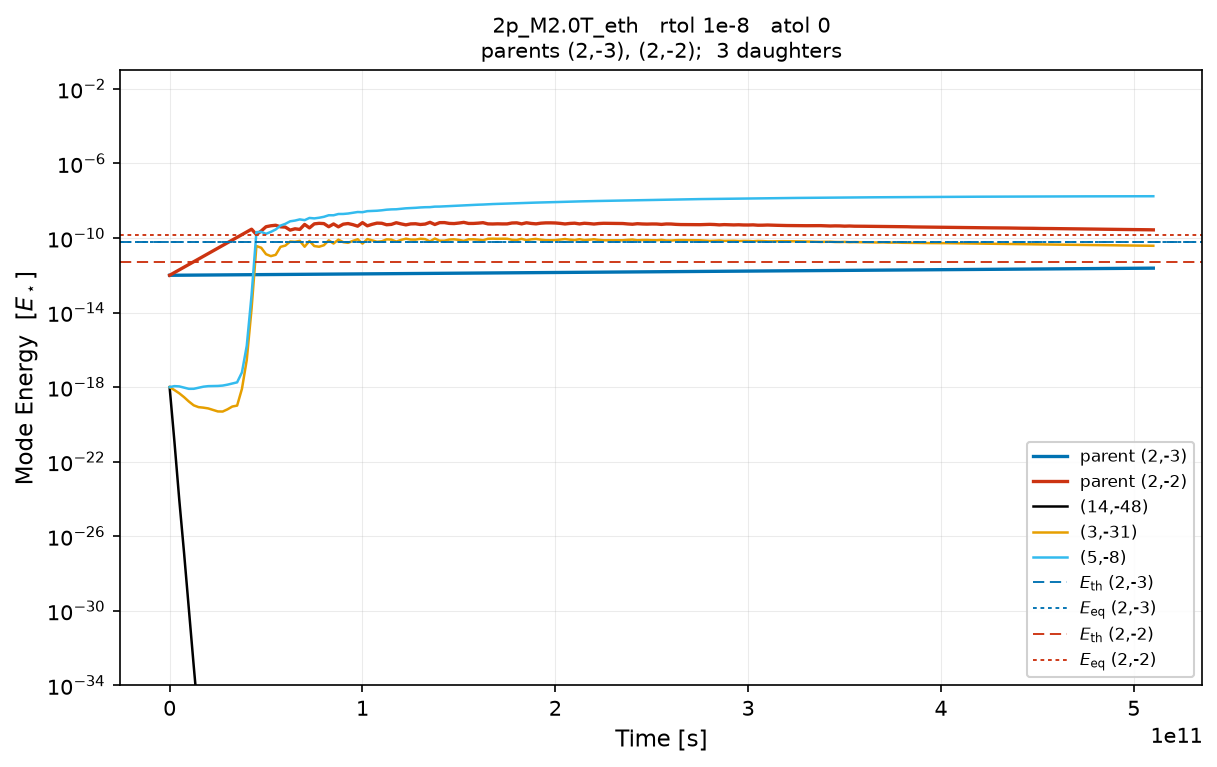
\includegraphics[width=0.21\textwidth,height=0.1323\textwidth]{../plots/rk8pd/2p_M2.0T_eth/r1e-8_a0.png} \\[-1pt]
 & \parbox[t]{0.21\textwidth}{\centering\scriptsize 385.6\,k steps, 1.5\,s} & \parbox[t]{0.21\textwidth}{\centering\scriptsize 385.4\,k steps, 9.3\,s} & \parbox[t]{0.21\textwidth}{\centering\scriptsize 385.4\,k steps, 2.4\,s} & \parbox[t]{0.21\textwidth}{\centering\scriptsize 50.17\,M steps, 1522.6\,s, wall} \\[2pt]
\rotatebox{90}{\parbox{0.1323\textwidth}{\centering\scriptsize\bfseries BDF, dense analytic Jacobian}} & 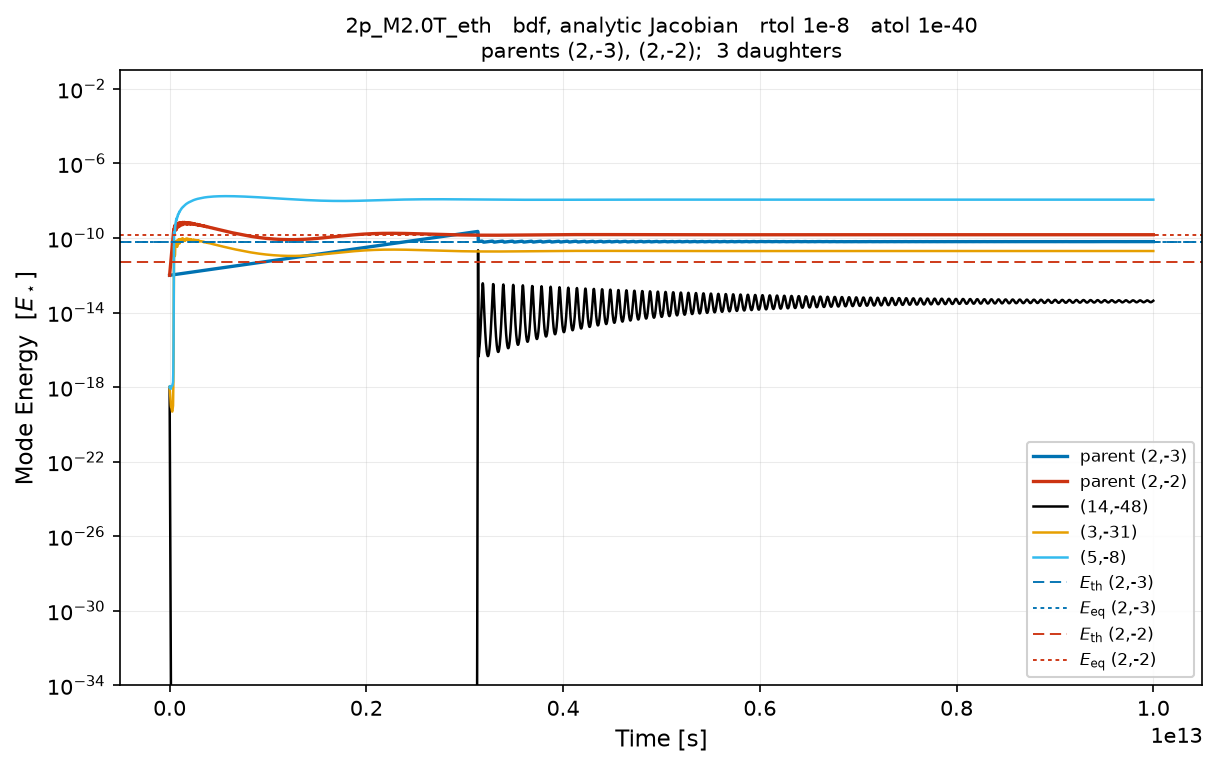
\includegraphics[width=0.21\textwidth,height=0.1323\textwidth]{../plots/bdf/2p_M2.0T_eth/r1e-8_a1e-40.png} & 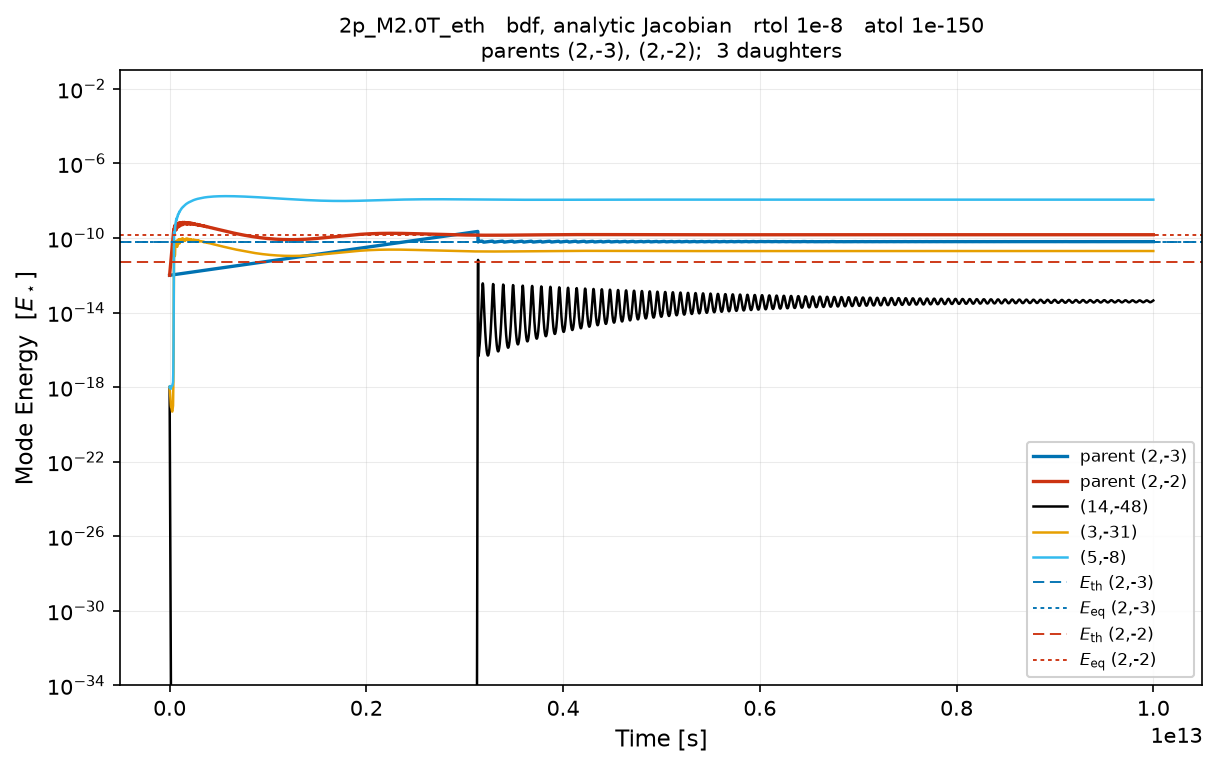
\includegraphics[width=0.21\textwidth,height=0.1323\textwidth]{../plots/bdf/2p_M2.0T_eth/r1e-8_a1e-150.png} & 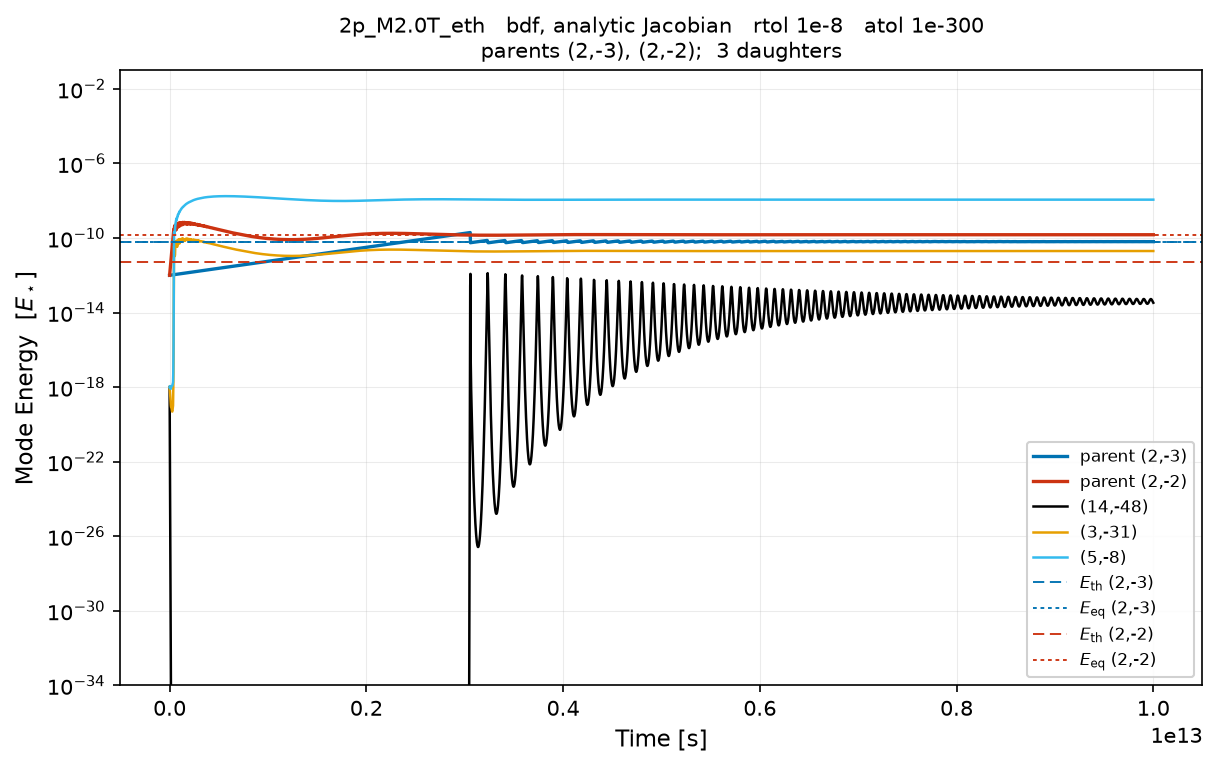
\includegraphics[width=0.21\textwidth,height=0.1323\textwidth]{../plots/bdf/2p_M2.0T_eth/r1e-8_a1e-300.png} & 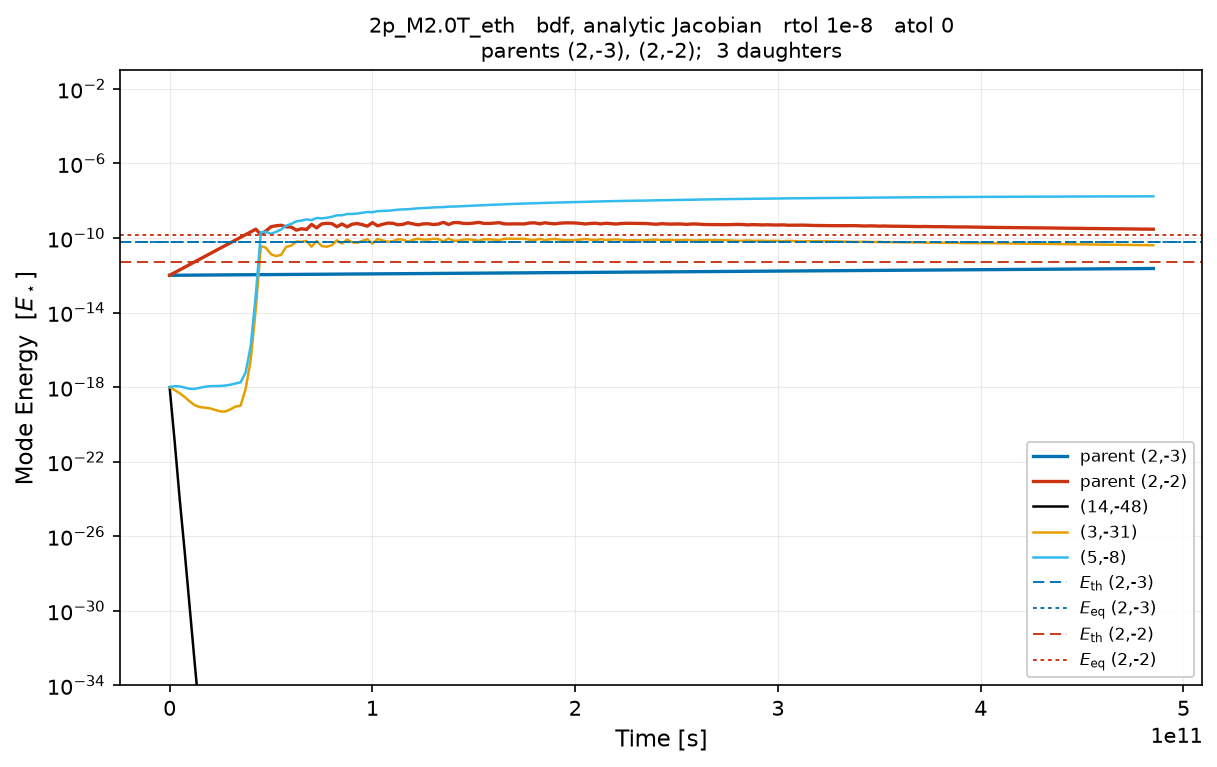
\includegraphics[width=0.21\textwidth,height=0.1323\textwidth]{../plots/bdf/2p_M2.0T_eth/r1e-8_a0.png} \\[-1pt]
 & \parbox[t]{0.21\textwidth}{\centering\scriptsize 3.45\,M steps, 3.7\,s} & \parbox[t]{0.21\textwidth}{\centering\scriptsize 3.45\,M steps, 13.0\,s} & \parbox[t]{0.21\textwidth}{\centering\scriptsize 3.45\,M steps, 4.3\,s} & \parbox[t]{0.21\textwidth}{\centering\scriptsize 145.3\,k steps, 0.4\,s, failed} \\[2pt]
\rotatebox{90}{\parbox{0.1323\textwidth}{\centering\scriptsize\bfseries BDF-Krylov, band full}} & 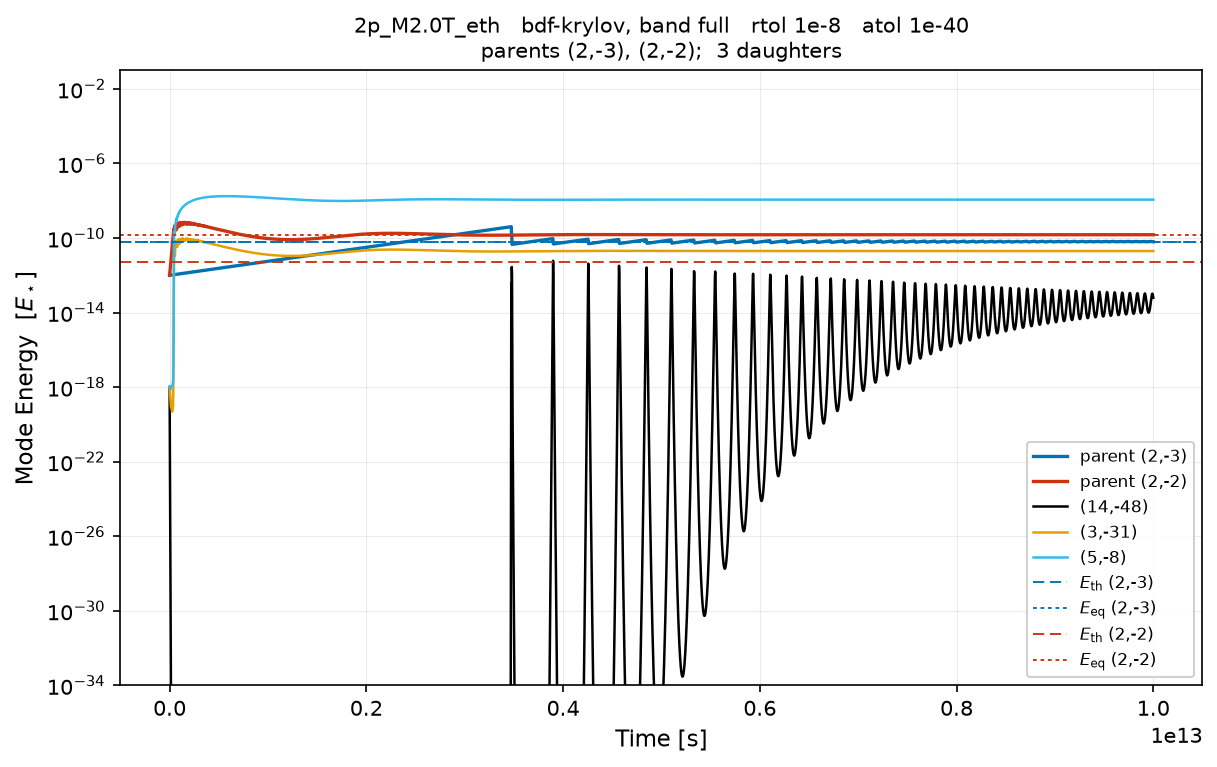
\includegraphics[width=0.21\textwidth,height=0.1323\textwidth]{../plots/krylov_full/2p_M2.0T_eth/r1e-8_a1e-40.png} & 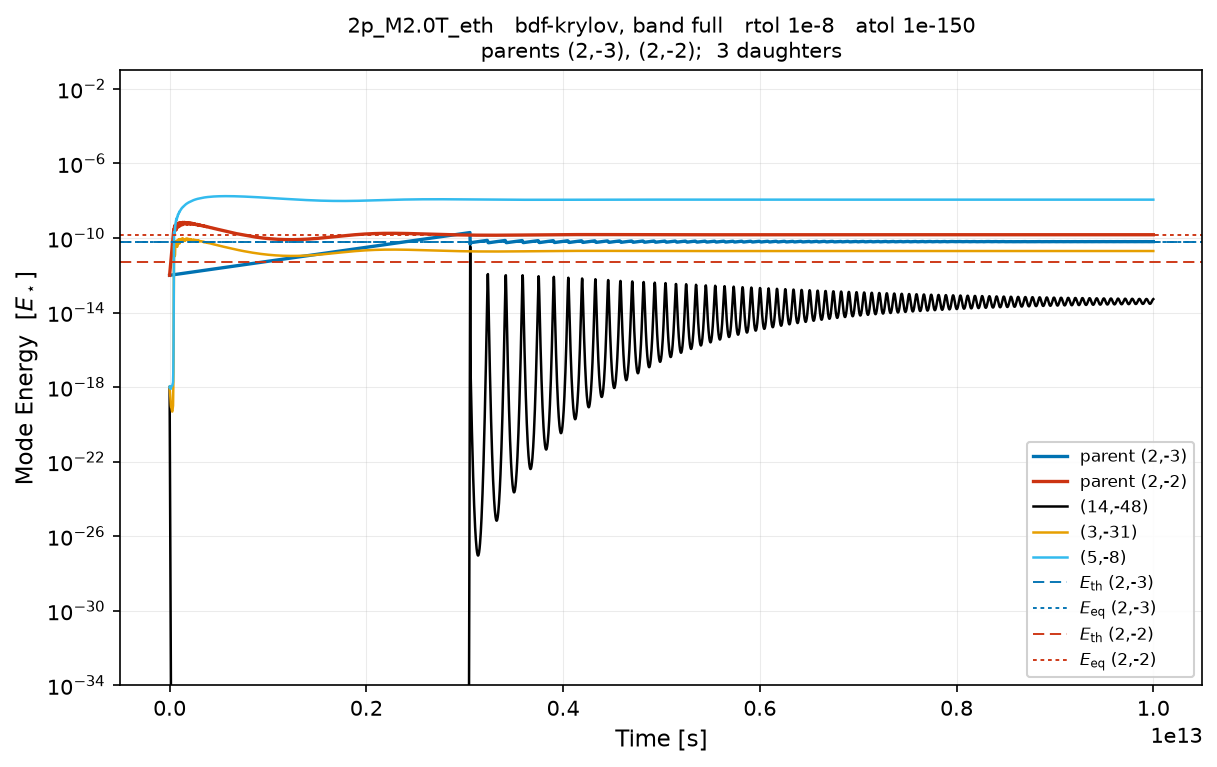
\includegraphics[width=0.21\textwidth,height=0.1323\textwidth]{../plots/krylov_full/2p_M2.0T_eth/r1e-8_a1e-150.png} & 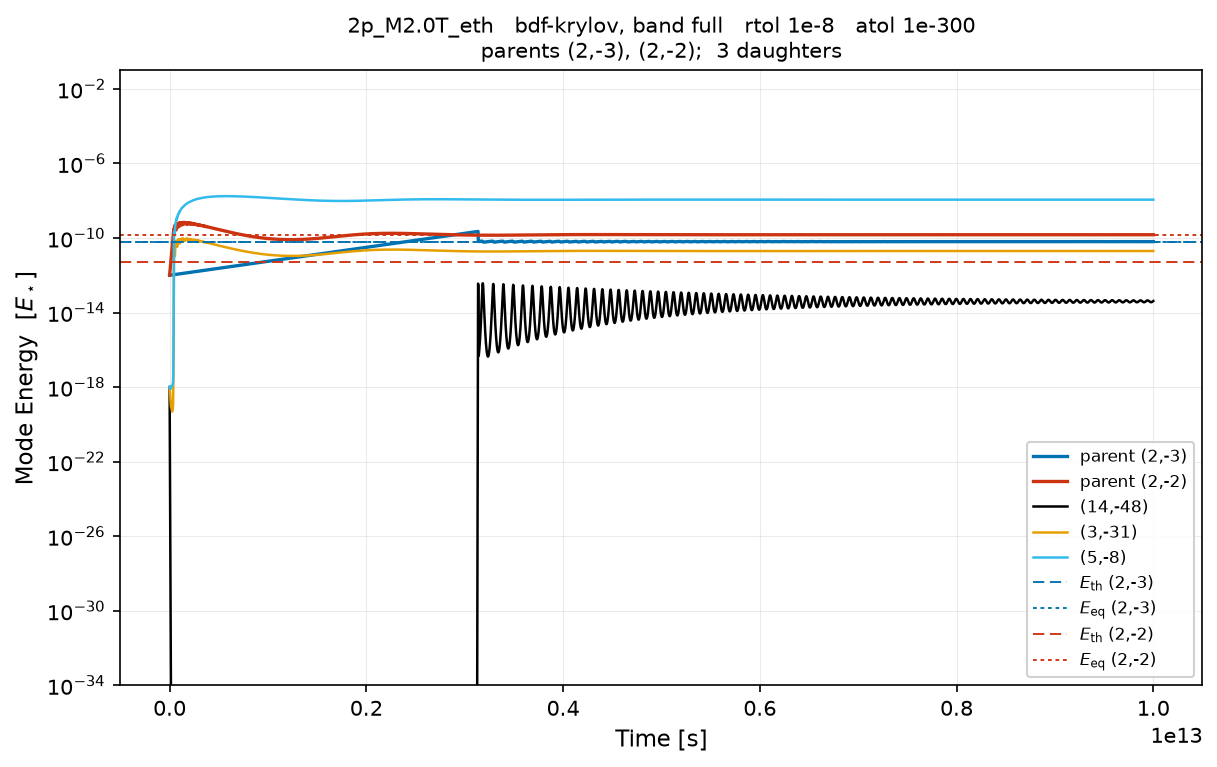
\includegraphics[width=0.21\textwidth,height=0.1323\textwidth]{../plots/krylov_full/2p_M2.0T_eth/r1e-8_a1e-300.png} & 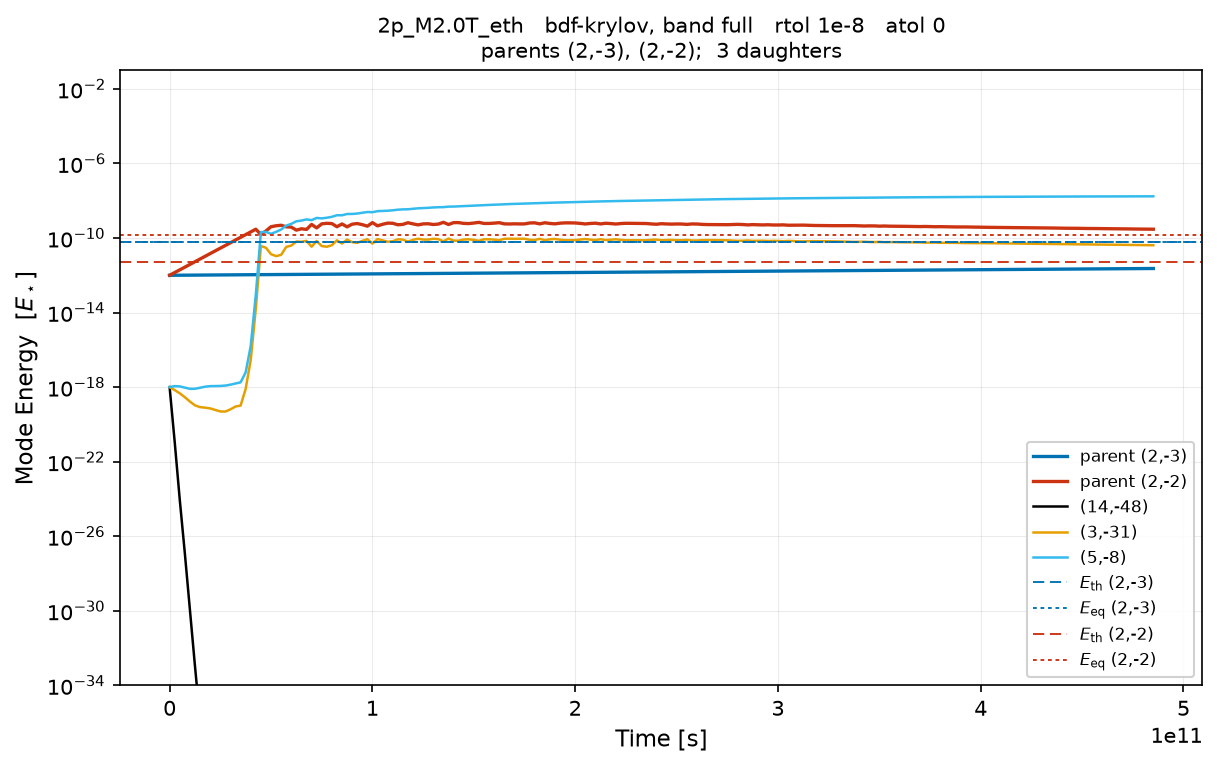
\includegraphics[width=0.21\textwidth,height=0.1323\textwidth]{../plots/krylov_full/2p_M2.0T_eth/r1e-8_a0.png} \\[-1pt]
 & \parbox[t]{0.21\textwidth}{\centering\scriptsize 3.41\,M steps, 10.0\,s} & \parbox[t]{0.21\textwidth}{\centering\scriptsize 3.40\,M steps, 7.4\,s} & \parbox[t]{0.21\textwidth}{\centering\scriptsize 3.41\,M steps, 18.4\,s} & \parbox[t]{0.21\textwidth}{\centering\scriptsize 143.2\,k steps, 0.6\,s, failed} \\[2pt]
\rotatebox{90}{\parbox{0.1323\textwidth}{\centering\scriptsize\bfseries BDF-Krylov, band 3}} & 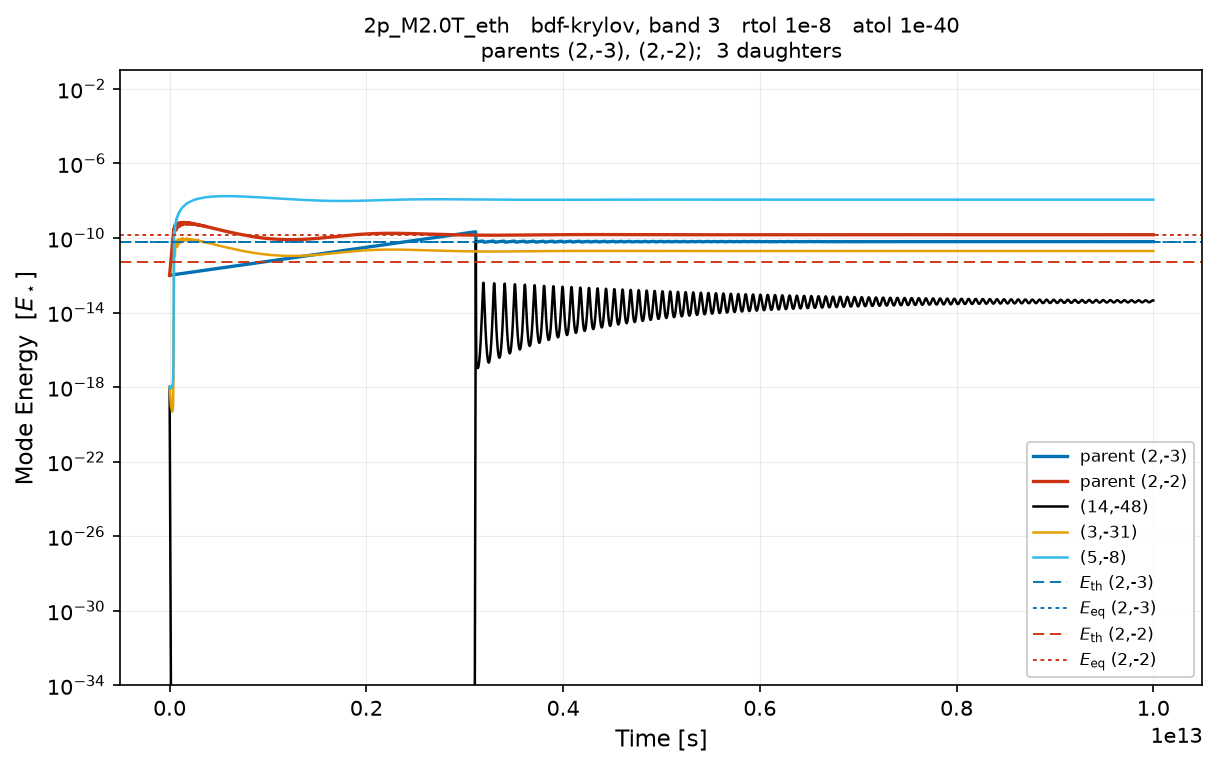
\includegraphics[width=0.21\textwidth,height=0.1323\textwidth]{../plots/krylov_b3/2p_M2.0T_eth/r1e-8_a1e-40.png} & 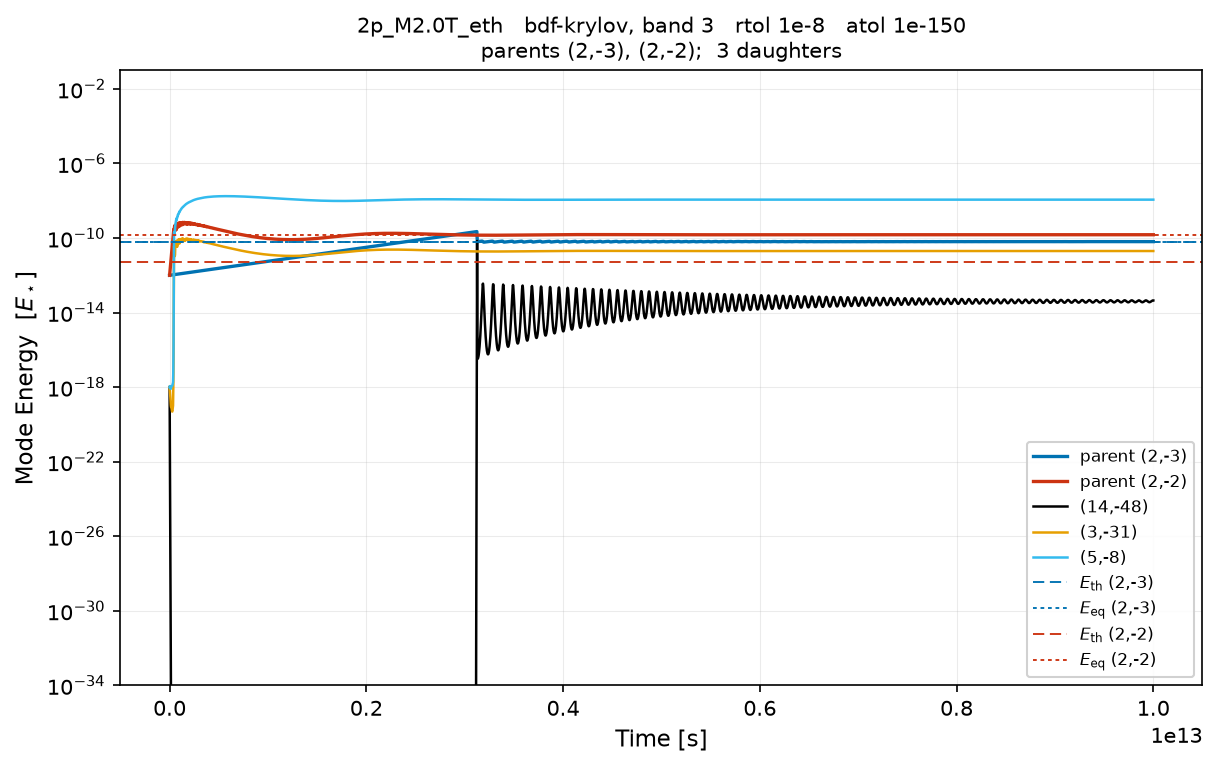
\includegraphics[width=0.21\textwidth,height=0.1323\textwidth]{../plots/krylov_b3/2p_M2.0T_eth/r1e-8_a1e-150.png} & 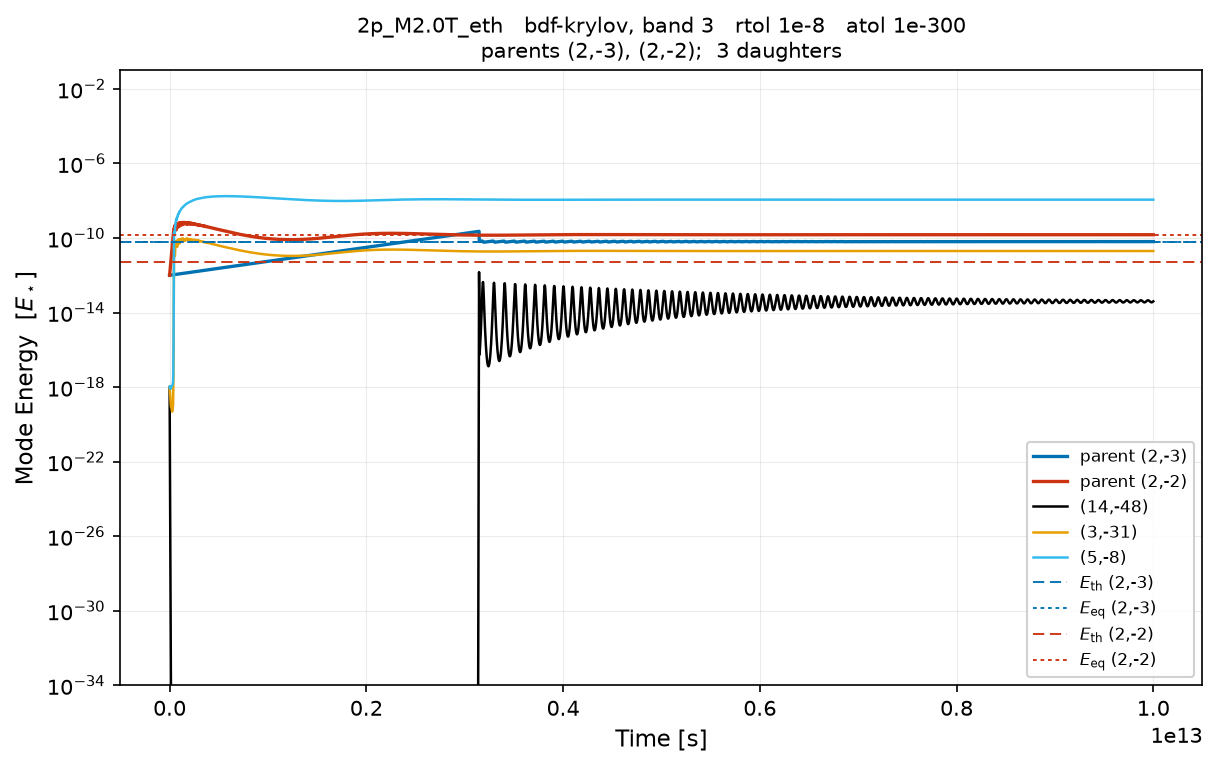
\includegraphics[width=0.21\textwidth,height=0.1323\textwidth]{../plots/krylov_b3/2p_M2.0T_eth/r1e-8_a1e-300.png} & 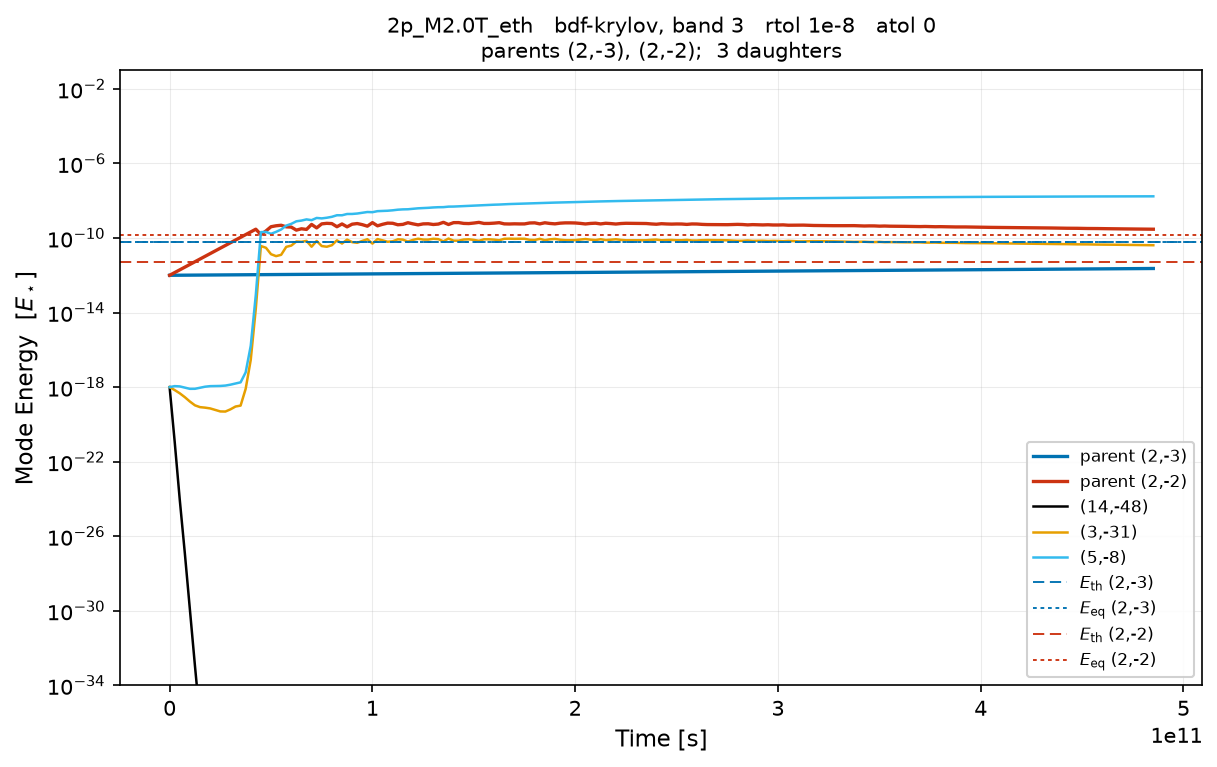
\includegraphics[width=0.21\textwidth,height=0.1323\textwidth]{../plots/krylov_b3/2p_M2.0T_eth/r1e-8_a0.png} \\[-1pt]
 & \parbox[t]{0.21\textwidth}{\centering\scriptsize 3.32\,M steps, 18.6\,s} & \parbox[t]{0.21\textwidth}{\centering\scriptsize 3.32\,M steps, 20.7\,s} & \parbox[t]{0.21\textwidth}{\centering\scriptsize 3.32\,M steps, 17.6\,s} & \parbox[t]{0.21\textwidth}{\centering\scriptsize 141.8\,k steps, 0.2\,s, failed} \\[2pt]
\rotatebox{90}{\parbox{0.1323\textwidth}{\centering\scriptsize\bfseries Adams, fixed point}} & 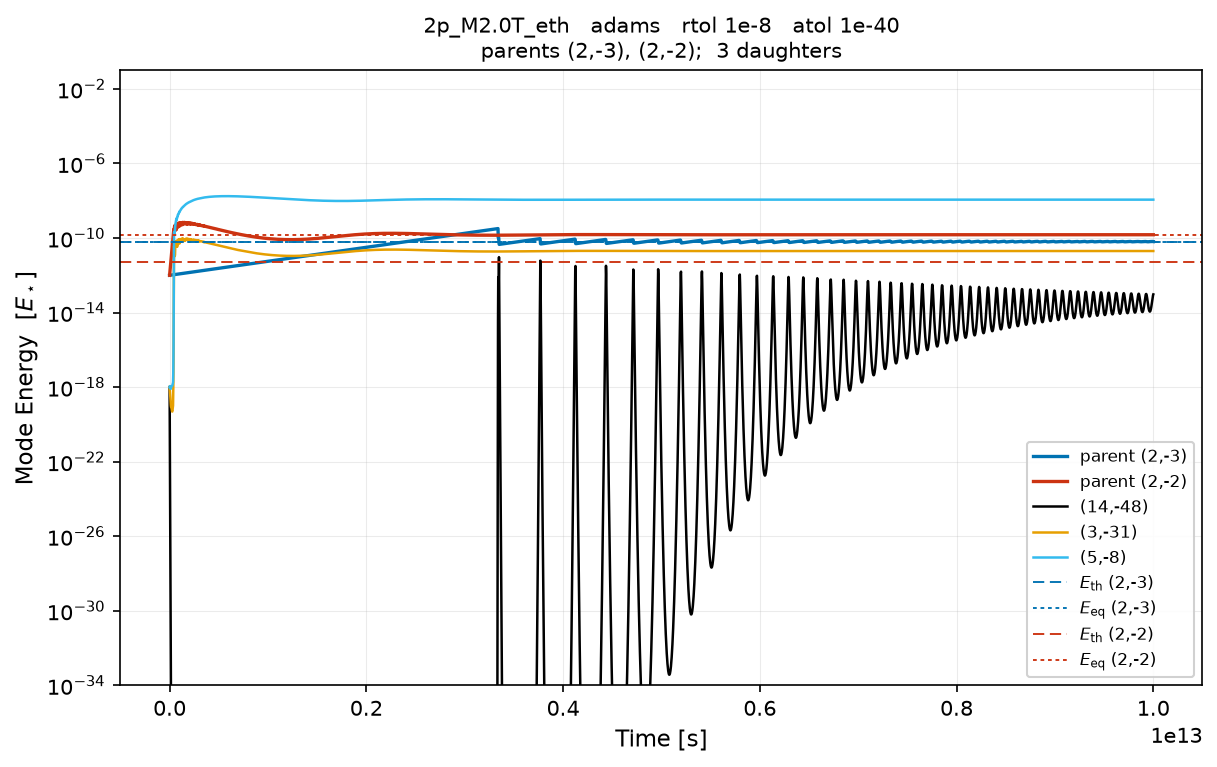
\includegraphics[width=0.21\textwidth,height=0.1323\textwidth]{../plots/adams/2p_M2.0T_eth/r1e-8_a1e-40.png} & 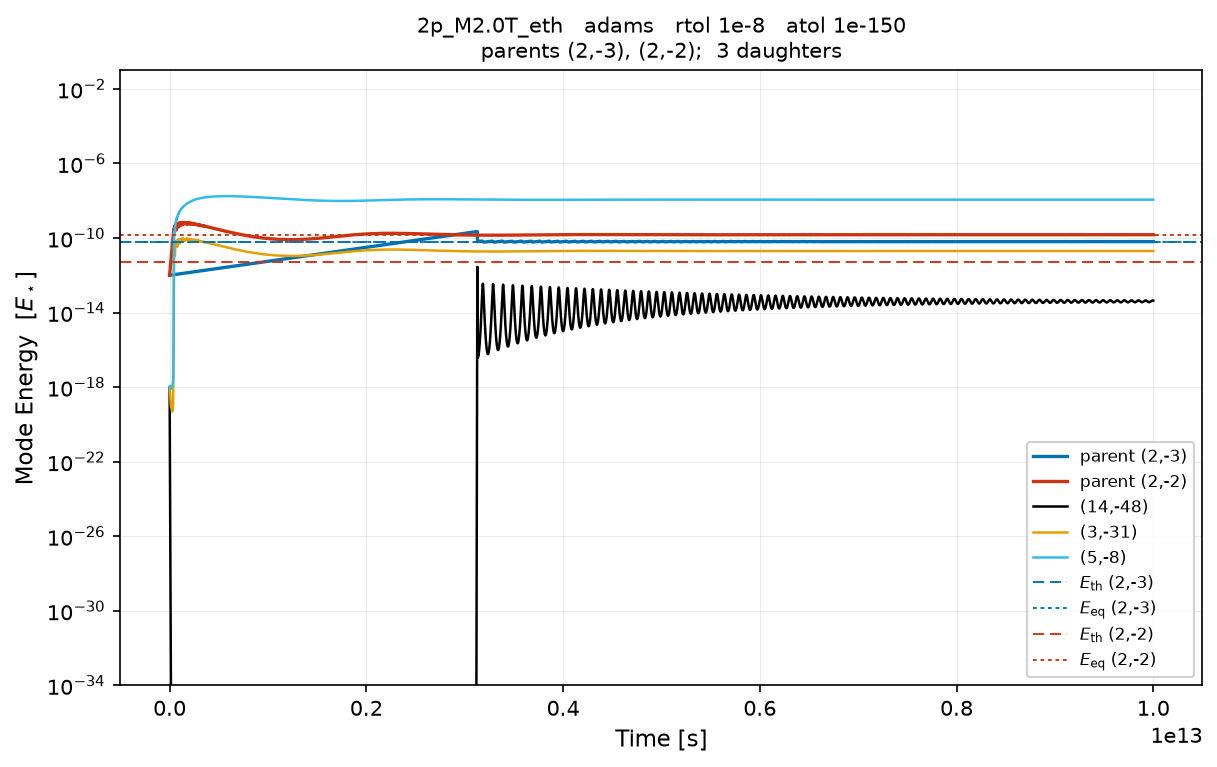
\includegraphics[width=0.21\textwidth,height=0.1323\textwidth]{../plots/adams/2p_M2.0T_eth/r1e-8_a1e-150.png} & 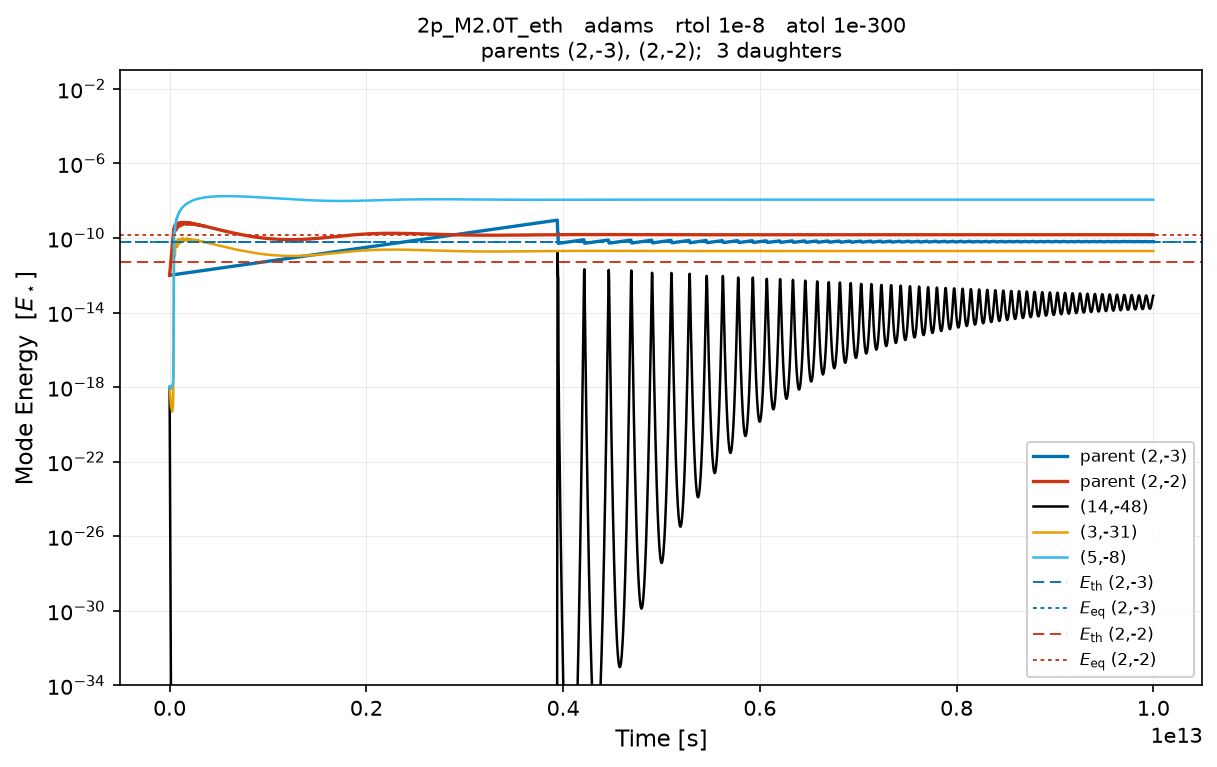
\includegraphics[width=0.21\textwidth,height=0.1323\textwidth]{../plots/adams/2p_M2.0T_eth/r1e-8_a1e-300.png} & 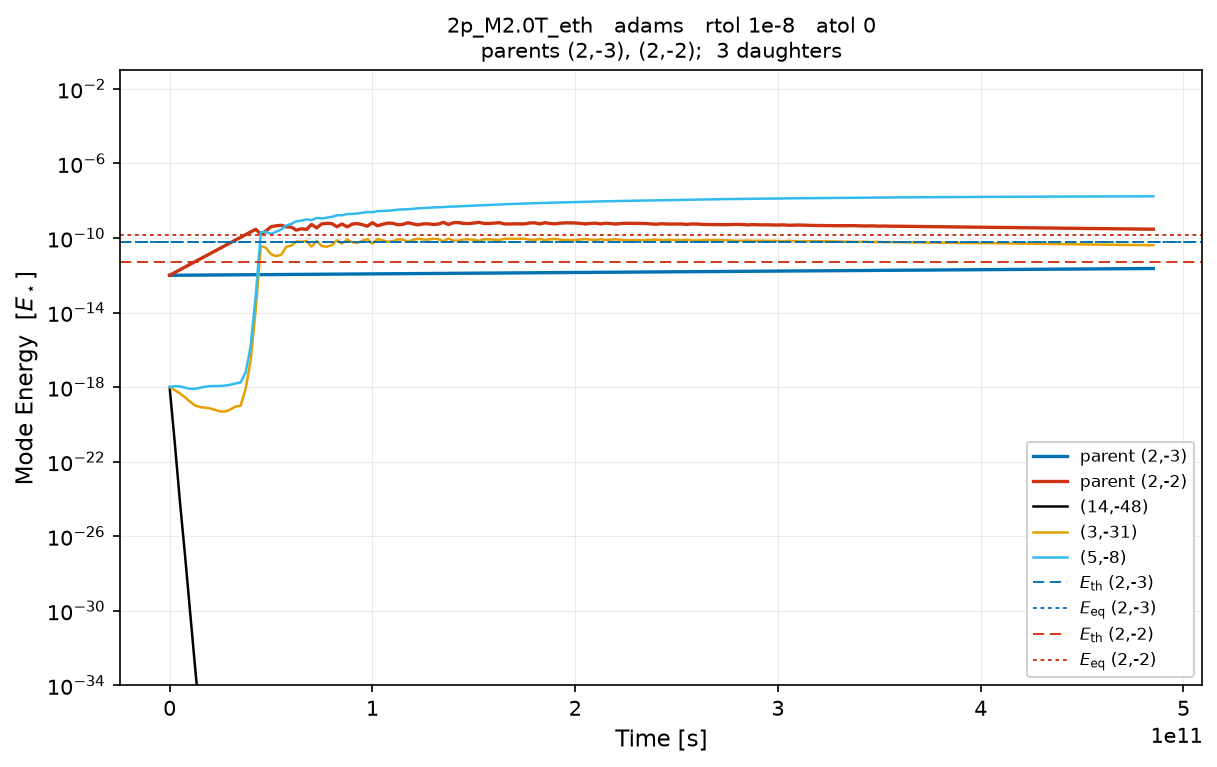
\includegraphics[width=0.21\textwidth,height=0.1323\textwidth]{../plots/adams/2p_M2.0T_eth/r1e-8_a0.png} \\[-1pt]
 & \parbox[t]{0.21\textwidth}{\centering\scriptsize 2.00\,M steps, 6.4\,s} & \parbox[t]{0.21\textwidth}{\centering\scriptsize 2.00\,M steps, 2.1\,s} & \parbox[t]{0.21\textwidth}{\centering\scriptsize 2.00\,M steps, 7.0\,s} & \parbox[t]{0.21\textwidth}{\centering\scriptsize 84.3\,k steps, 0.2\,s, failed} \\[2pt]
\end{tabular}\par}
\par\noindent{\scriptsize\setlength\tabcolsep{3.5pt}\renewcommand\arraystretch{0.92}
\begin{tabular}{@{}llllrrrrrrr@{}}
\toprule
integrator & atol & stop & $t_{\rm stop}$ [s] & steps & rejected & RHS & Jac. & NL it. & lin. it. & wall [s] \\
\midrule
rk8pd & $10^{-40}$ & end & $1.00\times10^{13}$ & 385.6\,k & 83.9\,k & 5.01\,M & -- & -- & -- & 1.5 \\
 & $10^{-150}$ & end & $1.00\times10^{13}$ & 385.4\,k & 83.7\,k & 5.01\,M & -- & -- & -- & 9.3 \\
 & $10^{-300}$ & end & $1.00\times10^{13}$ & 385.4\,k & 83.7\,k & 5.01\,M & -- & -- & -- & 2.4 \\
 & $0$ & wall & $5.10\times10^{11}$ & 50.17\,M & 56.1\,k & 652.18\,M & -- & -- & -- & 1522.6 \\
\addlinespace[2pt]
BDF, dense analytic Jacobian & $10^{-40}$ & end & $1.00\times10^{13}$ & 3.45\,M & 57.6\,k & 3.84\,M & 72.5\,k & 3.83\,M & -- & 3.7 \\
 & $10^{-150}$ & end & $1.00\times10^{13}$ & 3.45\,M & 57.4\,k & 3.84\,M & 72.5\,k & 3.83\,M & -- & 13.0 \\
 & $10^{-300}$ & end & $1.00\times10^{13}$ & 3.45\,M & 57.3\,k & 3.84\,M & 72.5\,k & 3.83\,M & -- & 4.3 \\
 & $0$ & failed & $4.85\times10^{11}$ & 145.3\,k & 3.9\,k & 167.3\,k & 3.2\,k & 167.1\,k & -- & 0.4 \\
\addlinespace[2pt]
BDF-Krylov, band full & $10^{-40}$ & end & $1.00\times10^{13}$ & 3.41\,M & 60.6\,k & 7.96\,M & 71.0\,k & 3.77\,M & 3.48\,M & 10.0 \\
 & $10^{-150}$ & end & $1.00\times10^{13}$ & 3.40\,M & 61.2\,k & 7.95\,M & 71.0\,k & 3.76\,M & 3.48\,M & 7.4 \\
 & $10^{-300}$ & end & $1.00\times10^{13}$ & 3.41\,M & 60.7\,k & 7.96\,M & 71.0\,k & 3.77\,M & 3.48\,M & 18.4 \\
 & $0$ & failed & $4.85\times10^{11}$ & 143.2\,k & 3.7\,k & 342.1\,k & 3.1\,k & 162.9\,k & 148.4\,k & 0.6 \\
\addlinespace[2pt]
BDF-Krylov, band 3 & $10^{-40}$ & end & $1.00\times10^{13}$ & 3.32\,M & 67.5\,k & 8.56\,M & 69.7\,k & 3.72\,M & 4.35\,M & 18.6 \\
 & $10^{-150}$ & end & $1.00\times10^{13}$ & 3.32\,M & 68.1\,k & 8.57\,M & 69.6\,k & 3.71\,M & 4.36\,M & 20.7 \\
 & $10^{-300}$ & end & $1.00\times10^{13}$ & 3.32\,M & 68.0\,k & 8.57\,M & 69.7\,k & 3.72\,M & 4.37\,M & 17.6 \\
 & $0$ & failed & $4.85\times10^{11}$ & 141.8\,k & 4.0\,k & 367.9\,k & 3.0\,k & 162.9\,k & 183.5\,k & 0.2 \\
\addlinespace[2pt]
Adams, fixed point & $10^{-40}$ & end & $1.00\times10^{13}$ & 2.00\,M & 131.7\,k & 3.30\,M & -- & 3.30\,M & -- & 6.4 \\
 & $10^{-150}$ & end & $1.00\times10^{13}$ & 2.00\,M & 132.1\,k & 3.30\,M & -- & 3.29\,M & -- & 2.1 \\
 & $10^{-300}$ & end & $1.00\times10^{13}$ & 2.00\,M & 132.3\,k & 3.30\,M & -- & 3.29\,M & -- & 7.0 \\
 & $0$ & failed & $4.85\times10^{11}$ & 84.3\,k & 5.9\,k & 138.5\,k & -- & 138.3\,k & -- & 0.2 \\
\bottomrule
\end{tabular}}

\clearpage
\subsection{\texttt{2p\_M2.0\_eeq}}\label{net:2p_M2.0_eeq}
\noindent\begin{minipage}[t]{0.43\textwidth}\vspace{0pt}\footnotesize
\begin{tabular}{@{}rrlrr@{}}
\toprule
id & gen & $(\ell,n)$ & $\omega$ [rad\,s$^{-1}$] & $\gamma$ [s$^{-1}$] \\
\midrule
0 & 0 & (1,$-$1) & $7.581\times10^{-4}$ & $-2.276\times10^{-10}$ \\
1 & 0 & (2,$-$2) & $7.710\times10^{-4}$ & $-1.619\times10^{-10}$ \\
2 & 1 & (5,$-$9) & $6.198\times10^{-4}$ & $4.584\times10^{-13}$ \\
3 & 1 & (6,$-$56) & $1.377\times10^{-4}$ & $2.817\times10^{-9}$ \\
4 & 1 & (6,$-$11) & $5.949\times10^{-4}$ & $1.643\times10^{-12}$ \\
5 & 1 & (8,$-$57) & $1.762\times10^{-4}$ & $4.129\times10^{-9}$ \\
\bottomrule
\end{tabular}
\end{minipage}\hfill
\begin{minipage}[t]{0.55\textwidth}\vspace{0pt}\footnotesize
\textbf{Model} \texttt{dsct\_M2.0}, rule eeq, $N=1$, cut 0.15,
closure 0.005; 6 modes, 2 triplet(s).\\[2pt]
\textbf{Selecting pairs}\\ (1,$-$1) $\to$ (5,$-$9) + (6,$-$56): $\Delta/\omega_a=-6.83\times10^{-4}$, $\kappa=+0.085$, $E_{\rm th}=1.75\times10^{-8}$, $E_{\rm eq}=2.07\times10^{-8}$\\
(2,$-$2) $\to$ (6,$-$11) + (8,$-$57): $\Delta/\omega_a=1.36\times10^{-4}$, $\kappa=+0.023$, $E_{\rm th}=1.97\times10^{-8}$, $E_{\rm eq}=2.13\times10^{-8}$\\[2pt]
Deep dips between bursts.
\end{minipage}

\par\smallskip{\centering\begin{tabular}{@{}c@{\hspace{2pt}}c@{\hspace{2pt}}c@{\hspace{2pt}}c@{\hspace{2pt}}c@{}}
 & \small atol $10^{-40}$ & \small atol $10^{-150}$ & \small atol $10^{-300}$ & \small atol $0$ \\[1pt]
\rotatebox{90}{\parbox{0.1323\textwidth}{\centering\scriptsize\bfseries rk8pd}} & 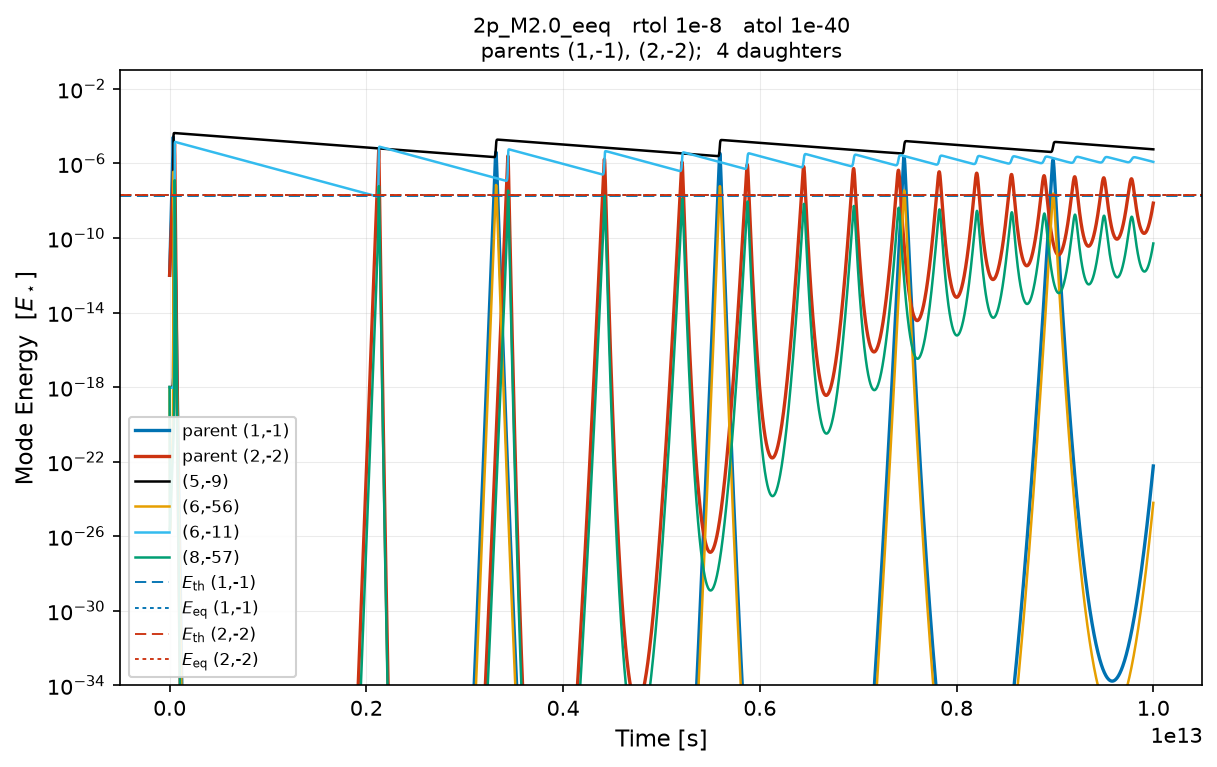
\includegraphics[width=0.21\textwidth,height=0.1323\textwidth]{../plots/rk8pd/2p_M2.0_eeq/r1e-8_a1e-40.png} & 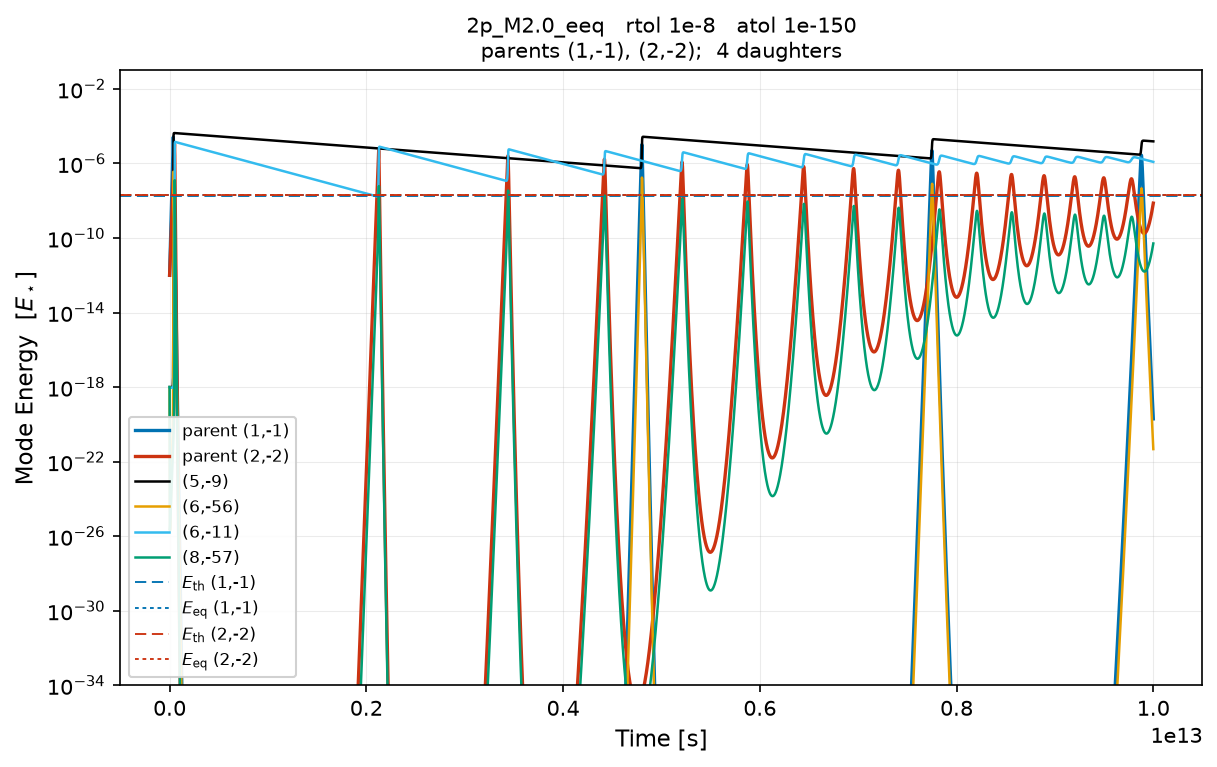
\includegraphics[width=0.21\textwidth,height=0.1323\textwidth]{../plots/rk8pd/2p_M2.0_eeq/r1e-8_a1e-150.png} & 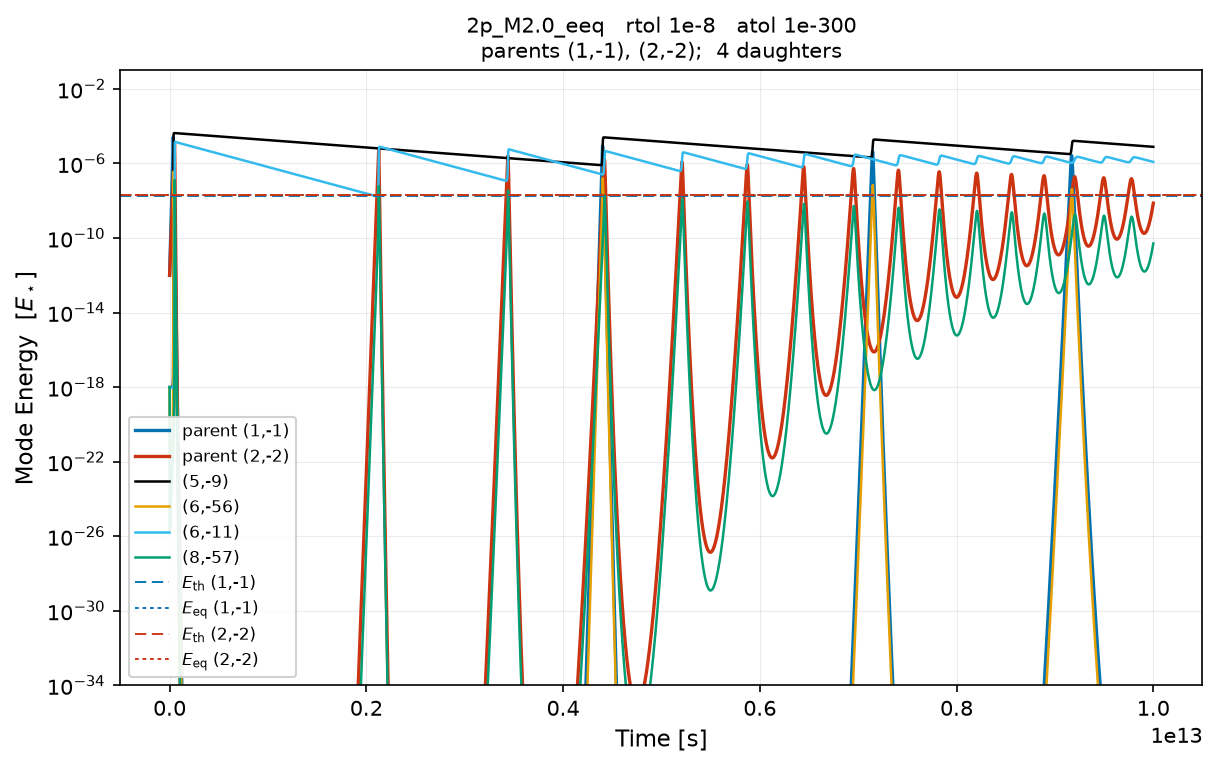
\includegraphics[width=0.21\textwidth,height=0.1323\textwidth]{../plots/rk8pd/2p_M2.0_eeq/r1e-8_a1e-300.png} & 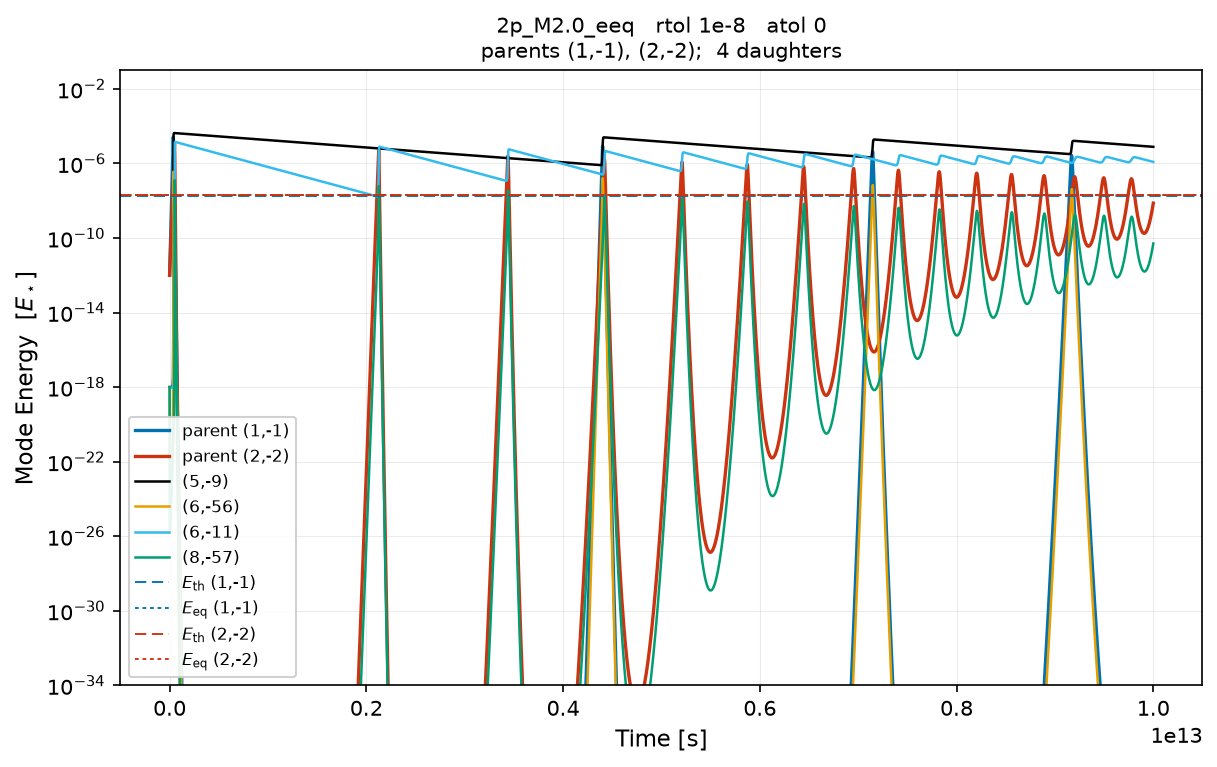
\includegraphics[width=0.21\textwidth,height=0.1323\textwidth]{../plots/rk8pd/2p_M2.0_eeq/r1e-8_a0.png} \\[-1pt]
 & \parbox[t]{0.21\textwidth}{\centering\scriptsize 6.11\,M steps, 16.3\,s} & \parbox[t]{0.21\textwidth}{\centering\scriptsize 8.12\,M steps, 35.2\,s} & \parbox[t]{0.21\textwidth}{\centering\scriptsize 9.27\,M steps, 35.6\,s} & \parbox[t]{0.21\textwidth}{\centering\scriptsize 9.27\,M steps, 32.1\,s} \\[2pt]
\rotatebox{90}{\parbox{0.1323\textwidth}{\centering\scriptsize\bfseries BDF, dense analytic Jacobian}} & 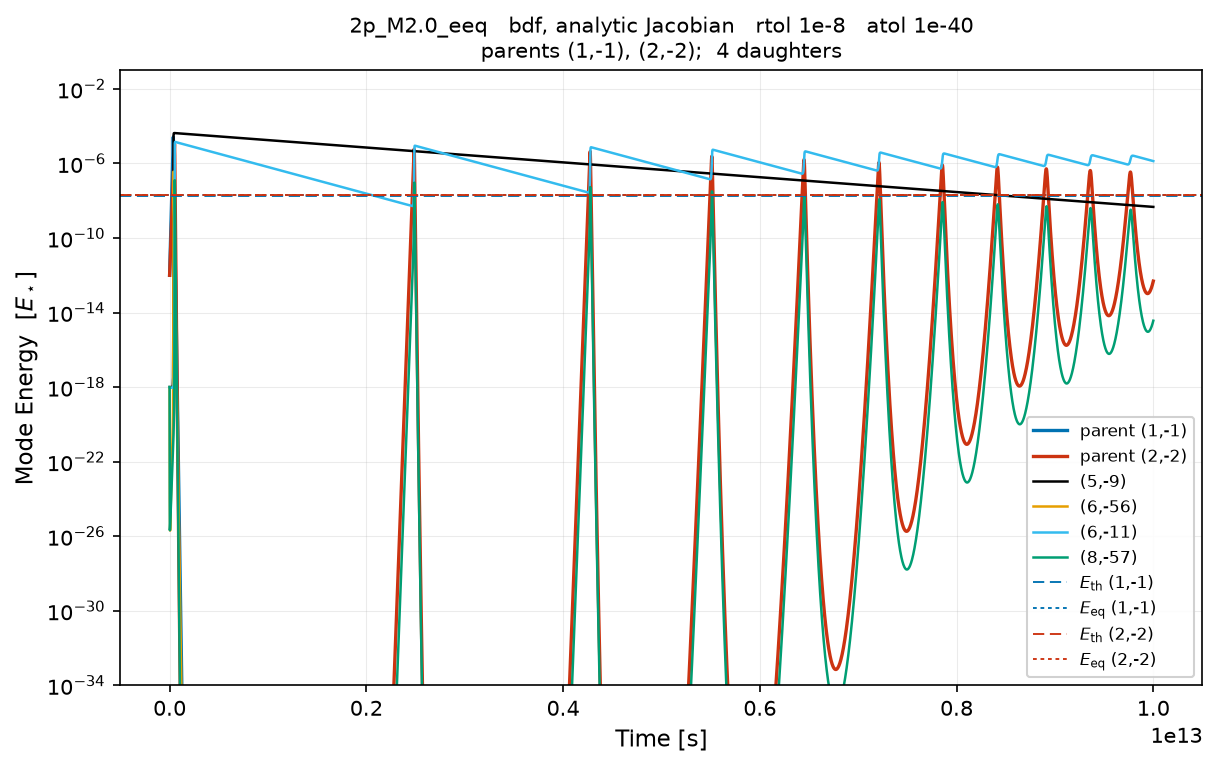
\includegraphics[width=0.21\textwidth,height=0.1323\textwidth]{../plots/bdf/2p_M2.0_eeq/r1e-8_a1e-40.png} & 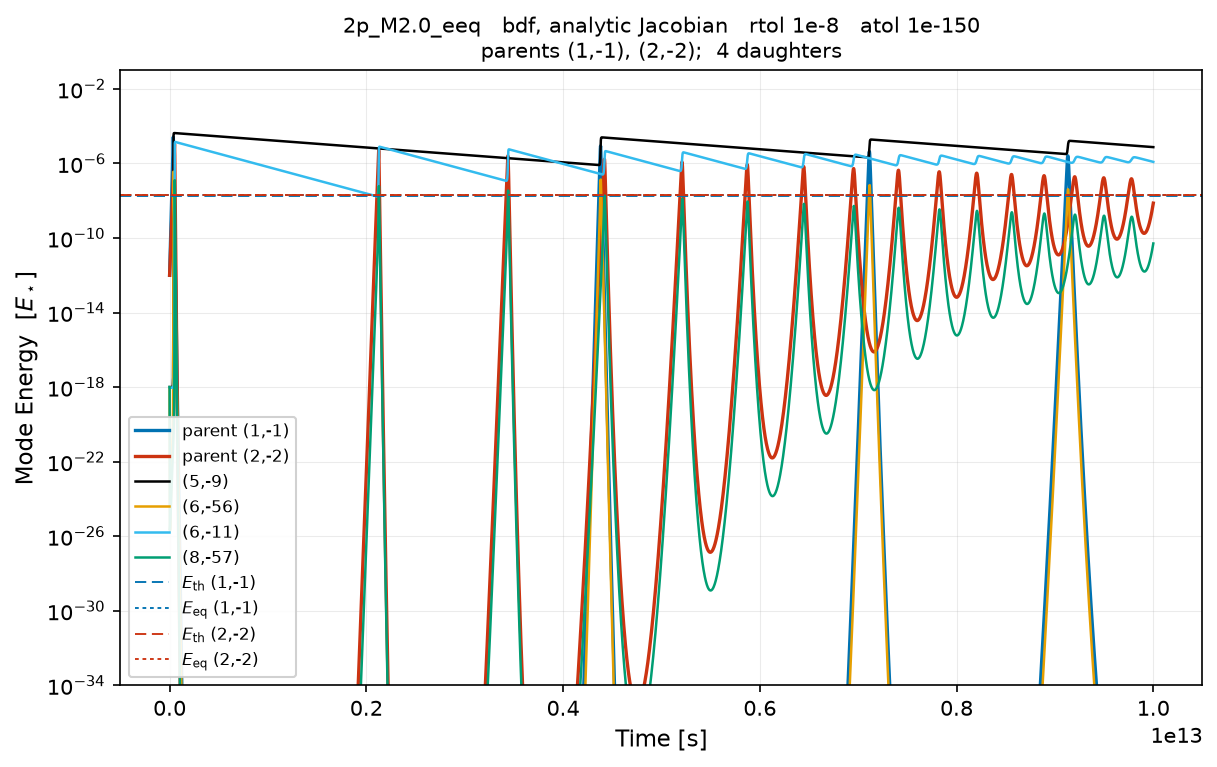
\includegraphics[width=0.21\textwidth,height=0.1323\textwidth]{../plots/bdf/2p_M2.0_eeq/r1e-8_a1e-150.png} & 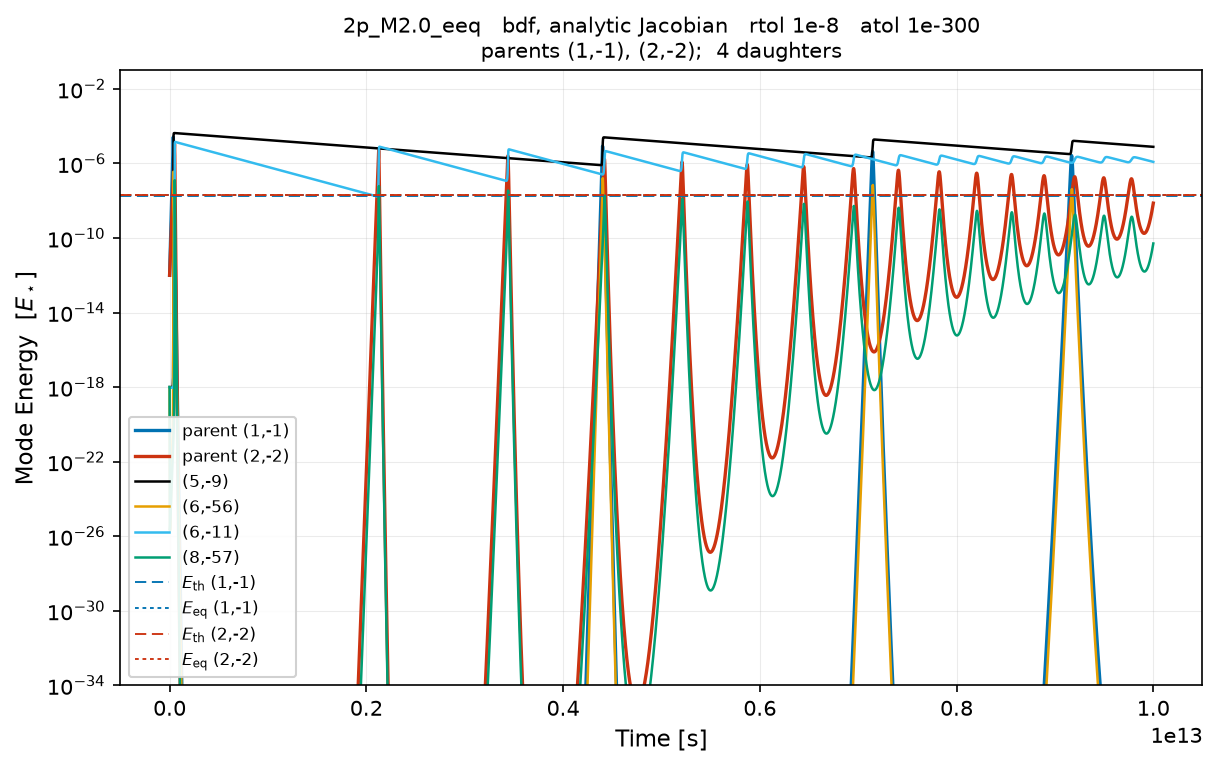
\includegraphics[width=0.21\textwidth,height=0.1323\textwidth]{../plots/bdf/2p_M2.0_eeq/r1e-8_a1e-300.png} & 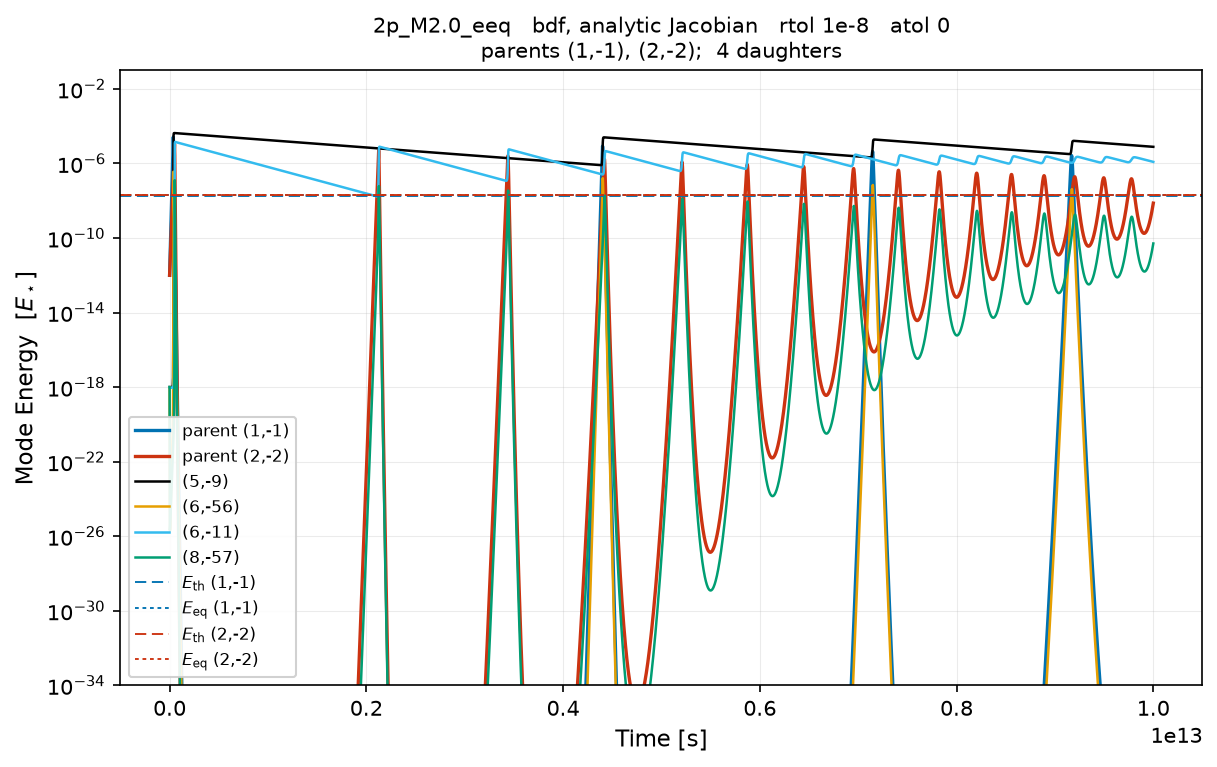
\includegraphics[width=0.21\textwidth,height=0.1323\textwidth]{../plots/bdf/2p_M2.0_eeq/r1e-8_a0.png} \\[-1pt]
 & \parbox[t]{0.21\textwidth}{\centering\scriptsize 18.35\,M steps, 102.8\,s} & \parbox[t]{0.21\textwidth}{\centering\scriptsize 107.34\,M steps, 157.1\,s} & \parbox[t]{0.21\textwidth}{\centering\scriptsize 114.65\,M steps, 193.2\,s} & \parbox[t]{0.21\textwidth}{\centering\scriptsize 114.65\,M steps, 183.6\,s} \\[2pt]
\rotatebox{90}{\parbox{0.1323\textwidth}{\centering\scriptsize\bfseries BDF-Krylov, band full}} & 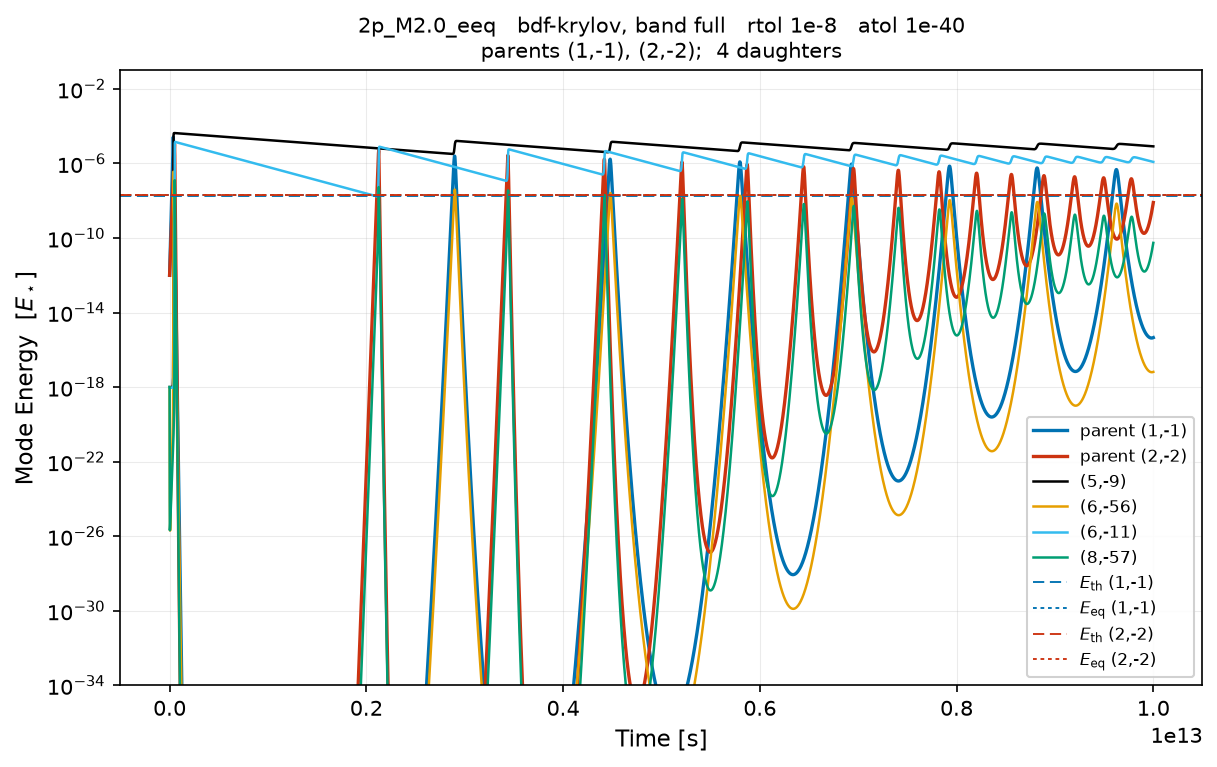
\includegraphics[width=0.21\textwidth,height=0.1323\textwidth]{../plots/krylov_full/2p_M2.0_eeq/r1e-8_a1e-40.png} & 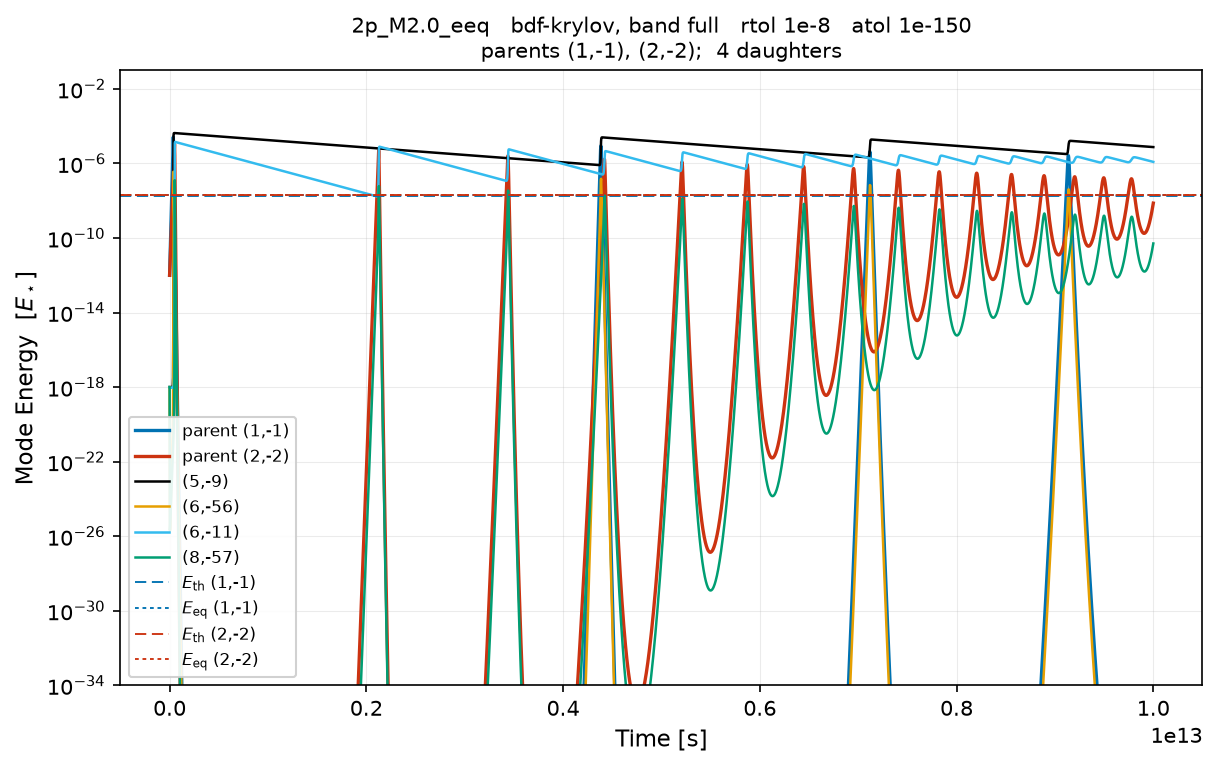
\includegraphics[width=0.21\textwidth,height=0.1323\textwidth]{../plots/krylov_full/2p_M2.0_eeq/r1e-8_a1e-150.png} & 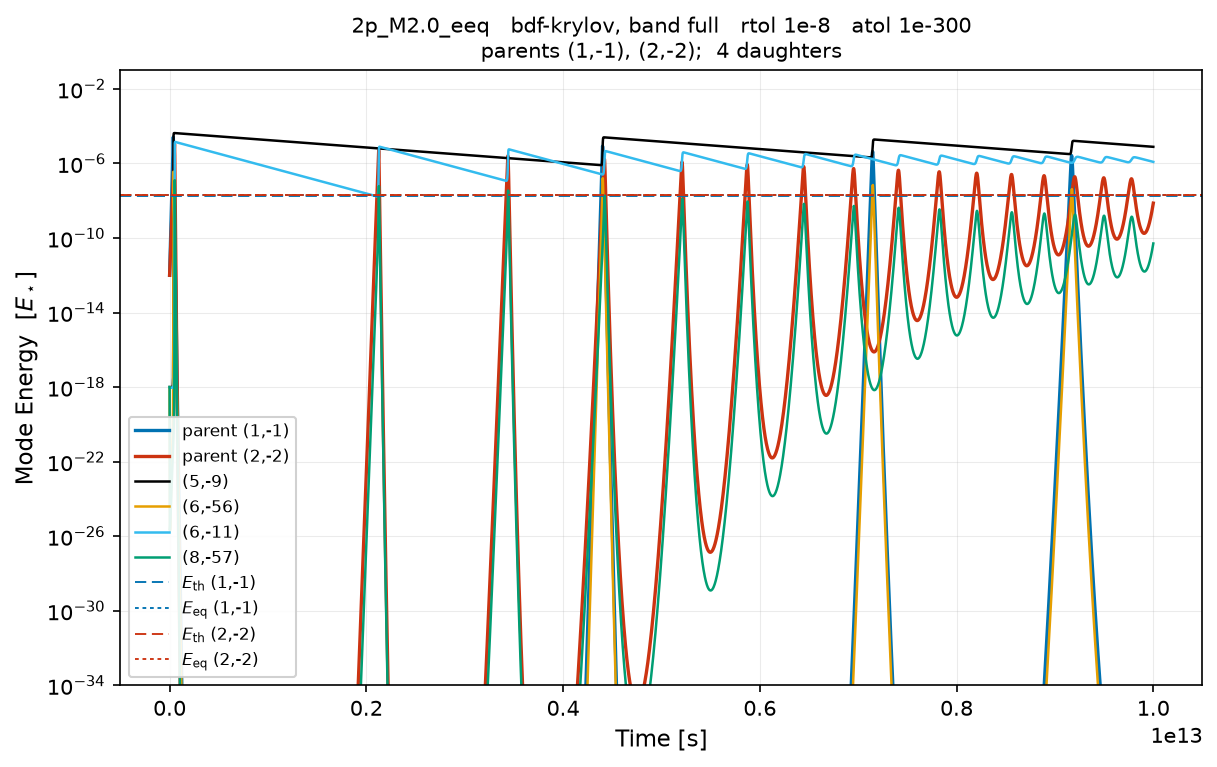
\includegraphics[width=0.21\textwidth,height=0.1323\textwidth]{../plots/krylov_full/2p_M2.0_eeq/r1e-8_a1e-300.png} & 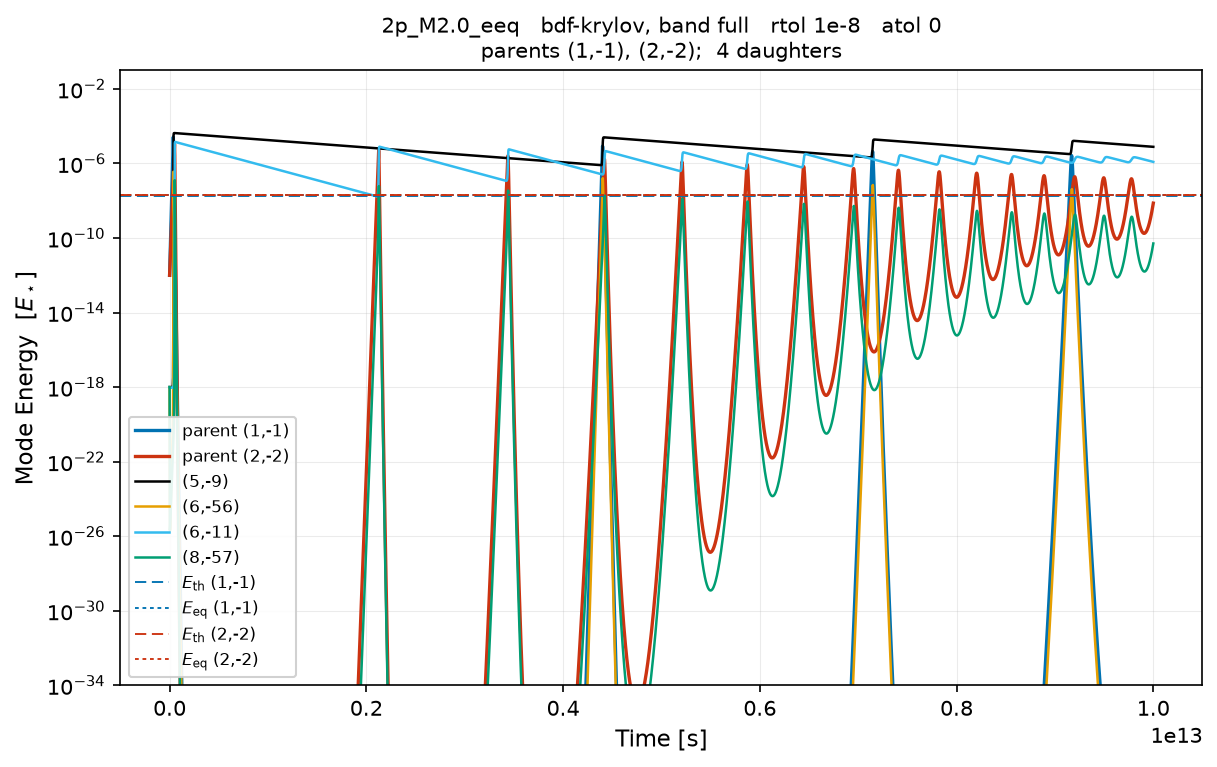
\includegraphics[width=0.21\textwidth,height=0.1323\textwidth]{../plots/krylov_full/2p_M2.0_eeq/r1e-8_a0.png} \\[-1pt]
 & \parbox[t]{0.21\textwidth}{\centering\scriptsize 94.11\,M steps, 215.5\,s} & \parbox[t]{0.21\textwidth}{\centering\scriptsize 103.74\,M steps, 217.1\,s} & \parbox[t]{0.21\textwidth}{\centering\scriptsize 110.66\,M steps, 213.7\,s} & \parbox[t]{0.21\textwidth}{\centering\scriptsize 110.66\,M steps, 219.8\,s} \\[2pt]
\rotatebox{90}{\parbox{0.1323\textwidth}{\centering\scriptsize\bfseries BDF-Krylov, band 3}} & 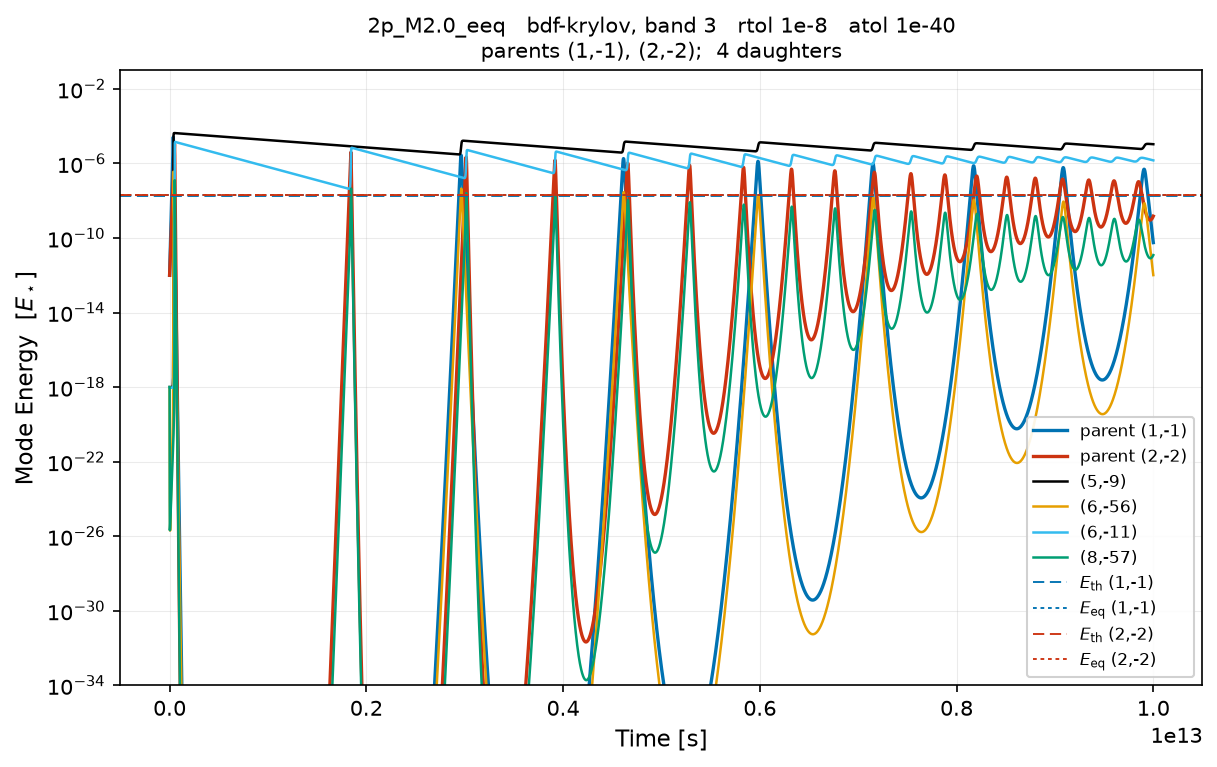
\includegraphics[width=0.21\textwidth,height=0.1323\textwidth]{../plots/krylov_b3/2p_M2.0_eeq/r1e-8_a1e-40.png} & 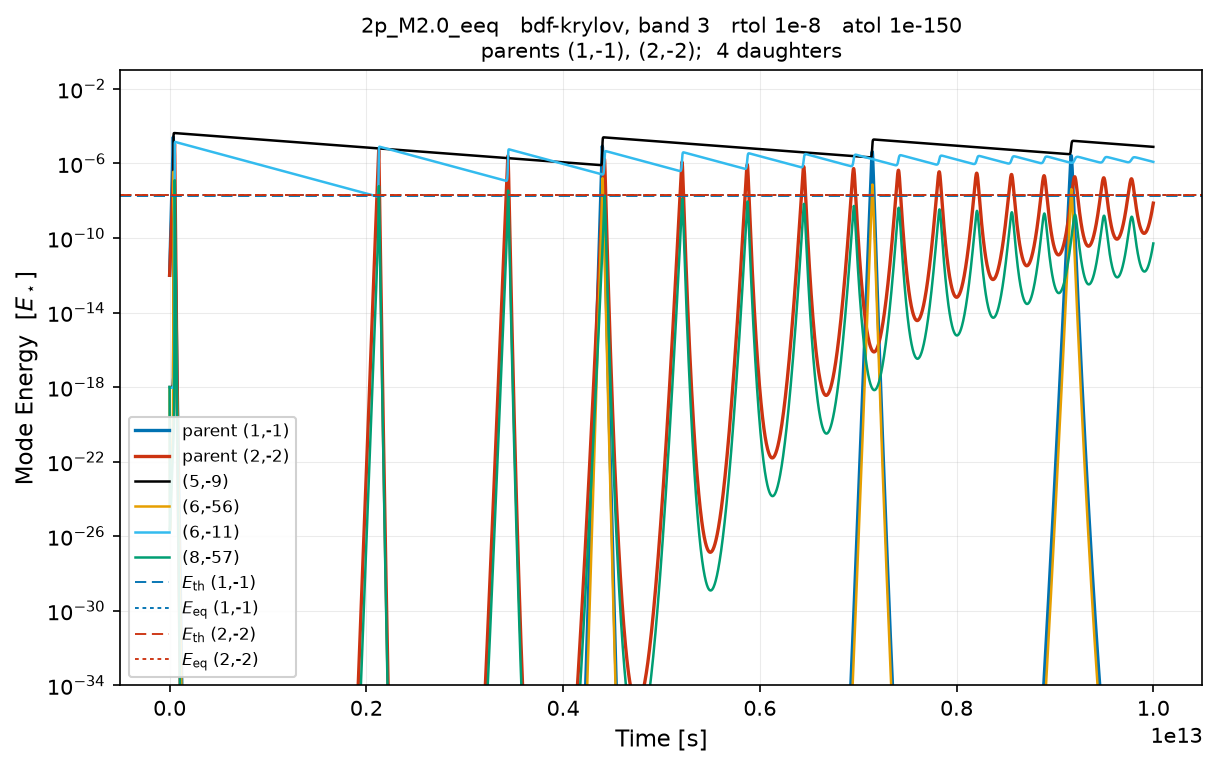
\includegraphics[width=0.21\textwidth,height=0.1323\textwidth]{../plots/krylov_b3/2p_M2.0_eeq/r1e-8_a1e-150.png} & 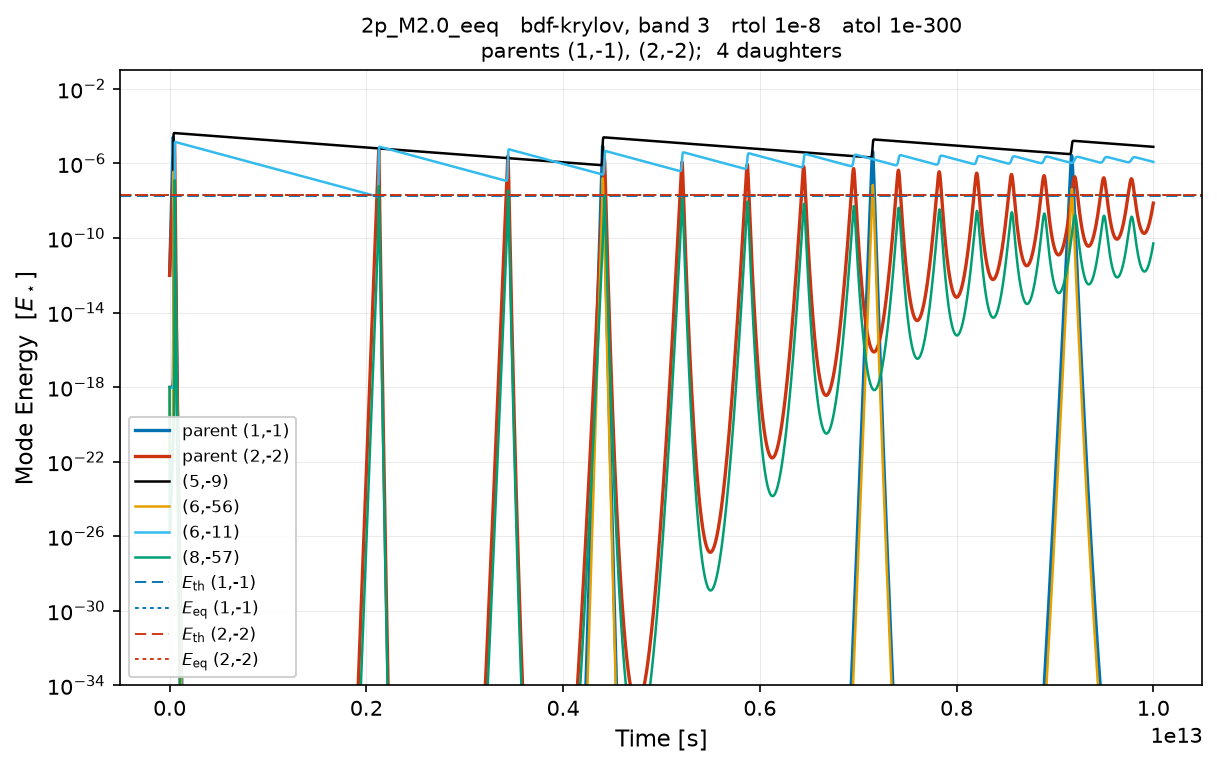
\includegraphics[width=0.21\textwidth,height=0.1323\textwidth]{../plots/krylov_b3/2p_M2.0_eeq/r1e-8_a1e-300.png} & 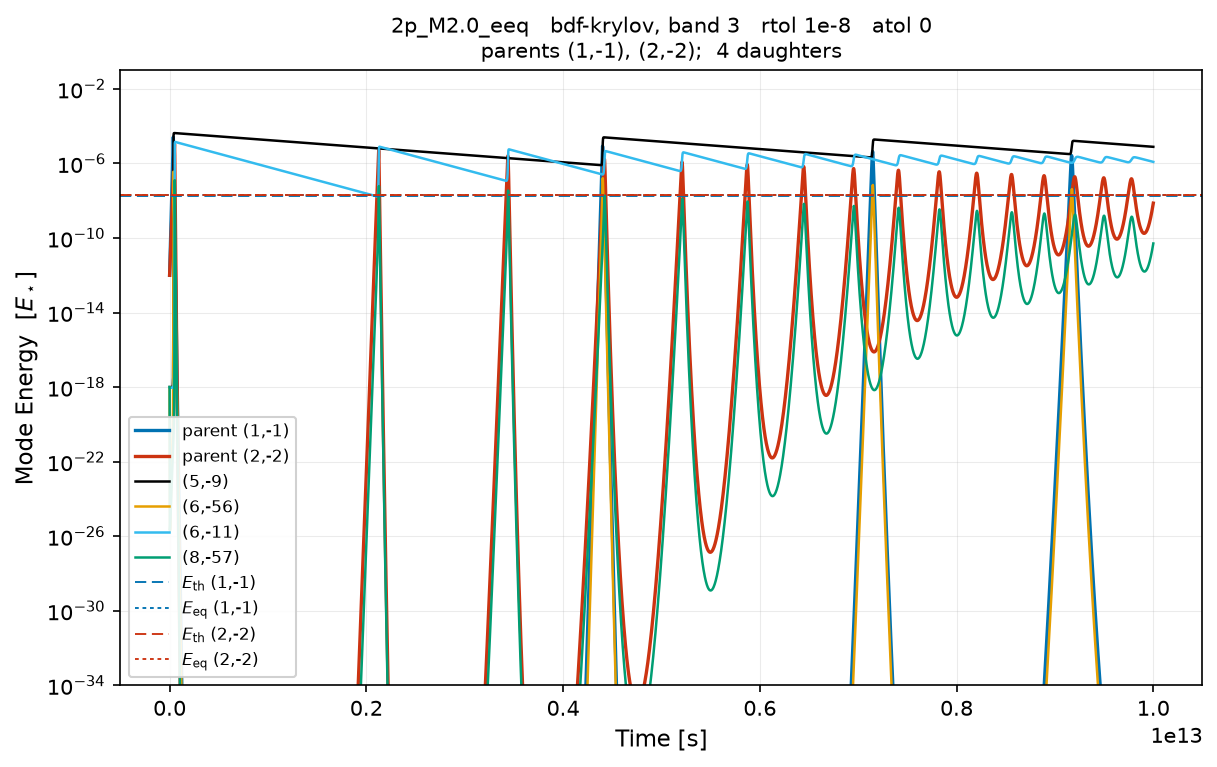
\includegraphics[width=0.21\textwidth,height=0.1323\textwidth]{../plots/krylov_b3/2p_M2.0_eeq/r1e-8_a0.png} \\[-1pt]
 & \parbox[t]{0.21\textwidth}{\centering\scriptsize 88.88\,M steps, 156.9\,s} & \parbox[t]{0.21\textwidth}{\centering\scriptsize 99.22\,M steps, 218.3\,s} & \parbox[t]{0.21\textwidth}{\centering\scriptsize 106.40\,M steps, 277.2\,s} & \parbox[t]{0.21\textwidth}{\centering\scriptsize 106.40\,M steps, 219.0\,s} \\[2pt]
\rotatebox{90}{\parbox{0.1323\textwidth}{\centering\scriptsize\bfseries Adams, fixed point}} & 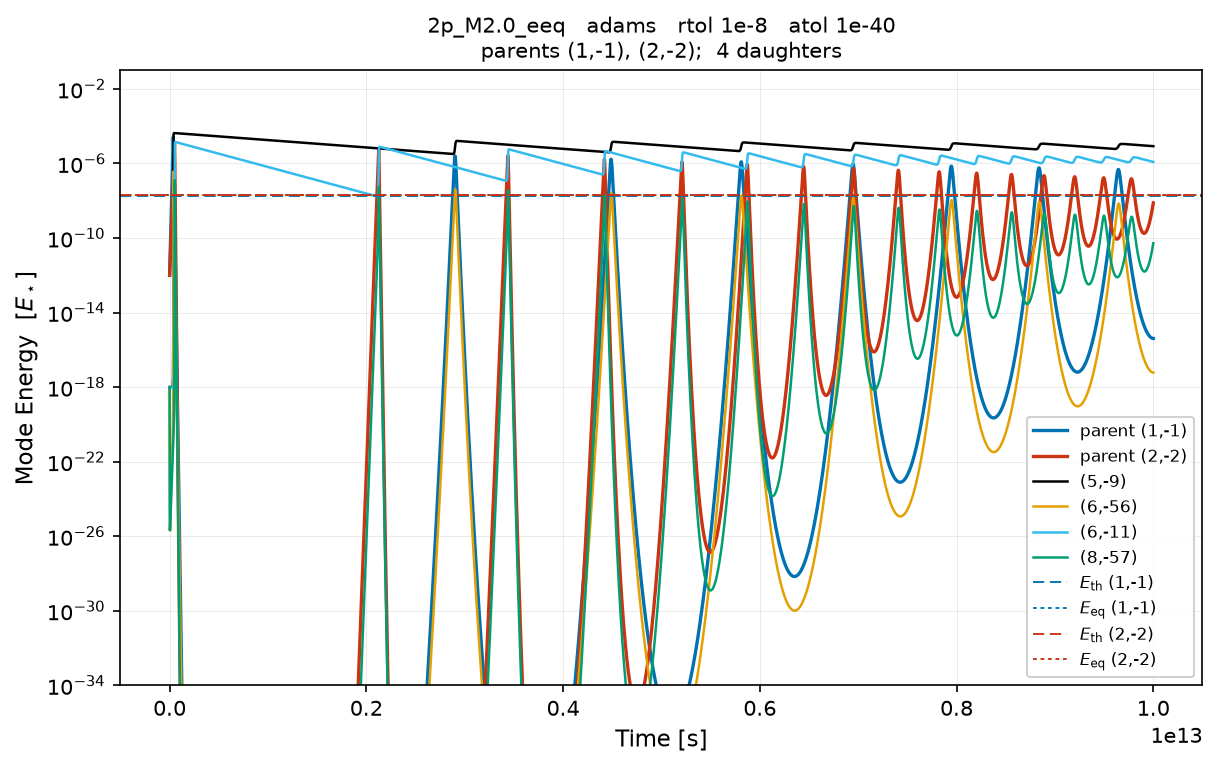
\includegraphics[width=0.21\textwidth,height=0.1323\textwidth]{../plots/adams/2p_M2.0_eeq/r1e-8_a1e-40.png} & 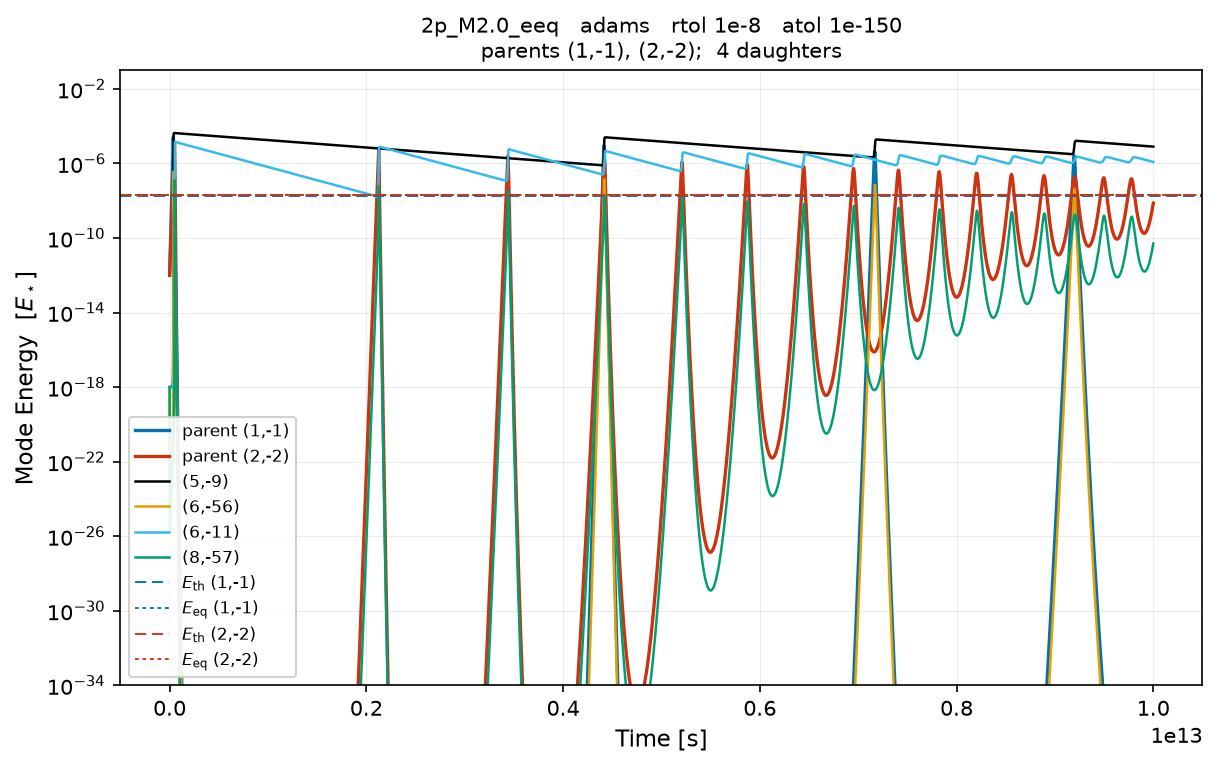
\includegraphics[width=0.21\textwidth,height=0.1323\textwidth]{../plots/adams/2p_M2.0_eeq/r1e-8_a1e-150.png} & 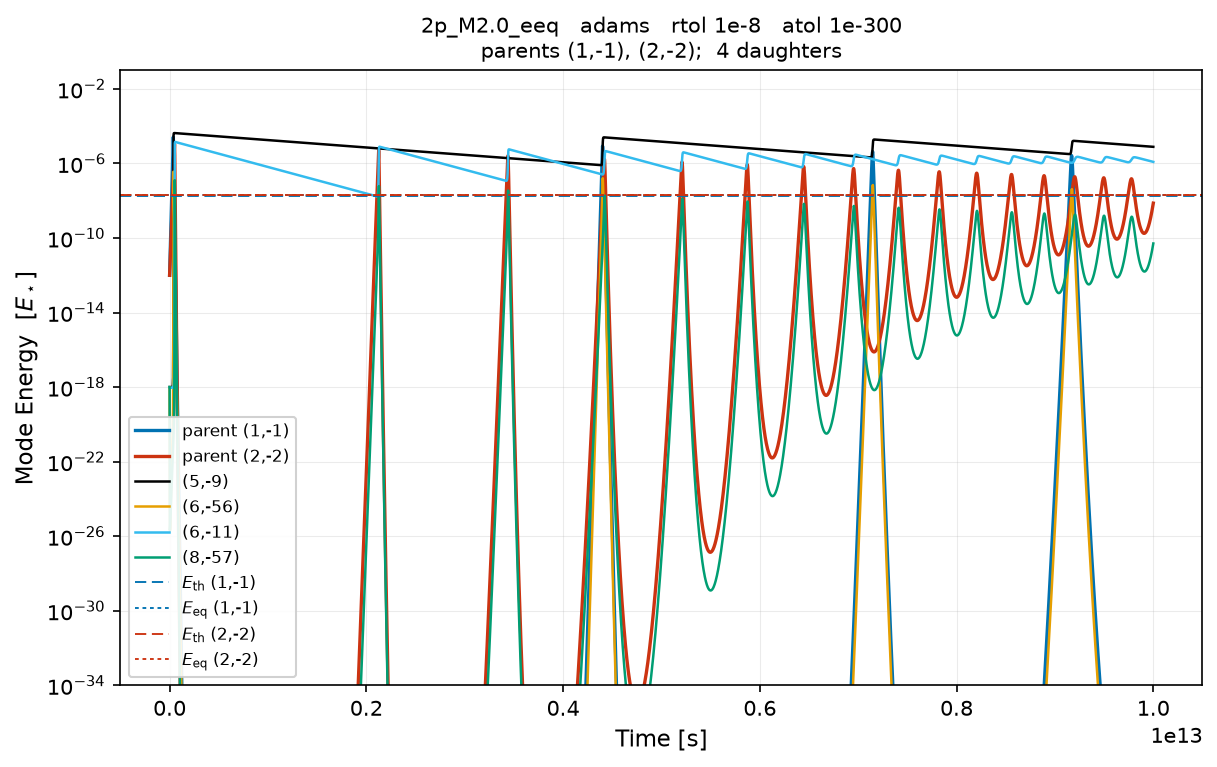
\includegraphics[width=0.21\textwidth,height=0.1323\textwidth]{../plots/adams/2p_M2.0_eeq/r1e-8_a1e-300.png} & 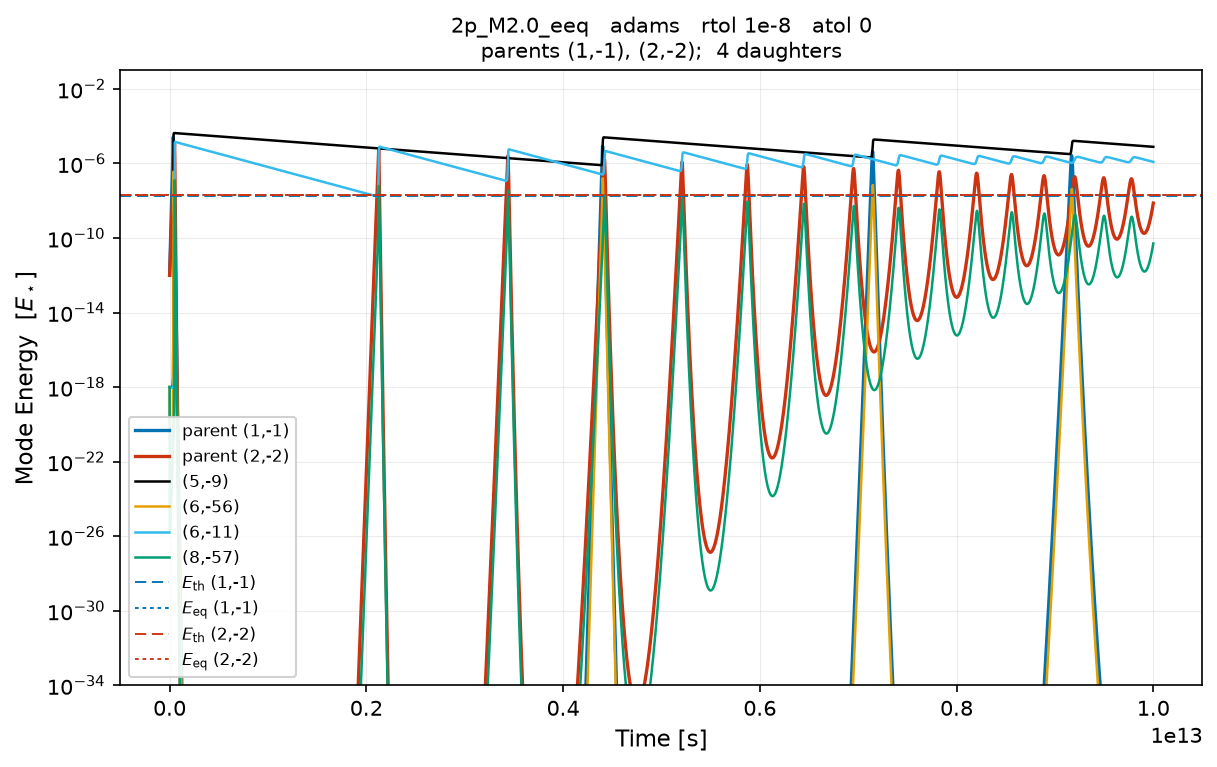
\includegraphics[width=0.21\textwidth,height=0.1323\textwidth]{../plots/adams/2p_M2.0_eeq/r1e-8_a0.png} \\[-1pt]
 & \parbox[t]{0.21\textwidth}{\centering\scriptsize 40.39\,M steps, 52.7\,s} & \parbox[t]{0.21\textwidth}{\centering\scriptsize 43.82\,M steps, 57.0\,s} & \parbox[t]{0.21\textwidth}{\centering\scriptsize 46.13\,M steps, 49.8\,s} & \parbox[t]{0.21\textwidth}{\centering\scriptsize 46.13\,M steps, 48.4\,s} \\[2pt]
\end{tabular}\par}
\par\noindent{\scriptsize\setlength\tabcolsep{3.5pt}\renewcommand\arraystretch{0.92}
\begin{tabular}{@{}llllrrrrrrr@{}}
\toprule
integrator & atol & stop & $t_{\rm stop}$ [s] & steps & rejected & RHS & Jac. & NL it. & lin. it. & wall [s] \\
\midrule
rk8pd & $10^{-40}$ & end & $1.00\times10^{13}$ & 6.11\,M & 535.4\,k & 79.40\,M & -- & -- & -- & 16.3 \\
 & $10^{-150}$ & end & $1.00\times10^{13}$ & 8.12\,M & 944.9\,k & 105.61\,M & -- & -- & -- & 35.2 \\
 & $10^{-300}$ & end & $1.00\times10^{13}$ & 9.27\,M & 1.04\,M & 120.46\,M & -- & -- & -- & 35.6 \\
 & $0$ & end & $1.00\times10^{13}$ & 9.27\,M & 1.04\,M & 120.46\,M & -- & -- & -- & 32.1 \\
\addlinespace[2pt]
BDF, dense analytic Jacobian & $10^{-40}$ & end & $1.00\times10^{13}$ & 18.35\,M & 206.2\,k & 20.00\,M & 382.9\,k & 20.00\,M & -- & 102.8 \\
 & $10^{-150}$ & end & $1.00\times10^{13}$ & 107.34\,M & 674.9\,k & 113.72\,M & 1.81\,M & 113.72\,M & -- & 157.1 \\
 & $10^{-300}$ & end & $1.00\times10^{13}$ & 114.65\,M & 735.3\,k & 121.52\,M & 1.93\,M & 121.52\,M & -- & 193.2 \\
 & $0$ & end & $1.00\times10^{13}$ & 114.65\,M & 735.3\,k & 121.52\,M & 1.93\,M & 121.52\,M & -- & 183.6 \\
\addlinespace[2pt]
BDF-Krylov, band full & $10^{-40}$ & end & $1.00\times10^{13}$ & 94.11\,M & 669.5\,k & 220.88\,M & 1.58\,M & 100.68\,M & 101.20\,M & 215.5 \\
 & $10^{-150}$ & end & $1.00\times10^{13}$ & 103.74\,M & 765.1\,k & 239.23\,M & 1.74\,M & 110.95\,M & 107.36\,M & 217.1 \\
 & $10^{-300}$ & end & $1.00\times10^{13}$ & 110.66\,M & 843.3\,k & 254.79\,M & 1.86\,M & 118.47\,M & 114.00\,M & 213.7 \\
 & $0$ & end & $1.00\times10^{13}$ & 110.66\,M & 843.3\,k & 254.79\,M & 1.86\,M & 118.47\,M & 114.00\,M & 219.8 \\
\addlinespace[2pt]
BDF-Krylov, band 3 & $10^{-40}$ & end & $1.00\times10^{13}$ & 88.88\,M & 917.3\,k & 219.52\,M & 1.50\,M & 96.67\,M & 112.37\,M & 156.9 \\
 & $10^{-150}$ & end & $1.00\times10^{13}$ & 99.22\,M & 1.06\,M & 241.99\,M & 1.67\,M & 107.98\,M & 122.31\,M & 218.3 \\
 & $10^{-300}$ & end & $1.00\times10^{13}$ & 106.40\,M & 1.15\,M & 258.82\,M & 1.79\,M & 115.88\,M & 130.40\,M & 277.2 \\
 & $0$ & end & $1.00\times10^{13}$ & 106.40\,M & 1.15\,M & 258.82\,M & 1.79\,M & 115.88\,M & 130.40\,M & 219.0 \\
\addlinespace[2pt]
Adams, fixed point & $10^{-40}$ & end & $1.00\times10^{13}$ & 40.39\,M & 1.44\,M & 58.85\,M & -- & 58.84\,M & -- & 52.7 \\
 & $10^{-150}$ & end & $1.00\times10^{13}$ & 43.82\,M & 1.91\,M & 64.54\,M & -- & 64.54\,M & -- & 57.0 \\
 & $10^{-300}$ & end & $1.00\times10^{13}$ & 46.13\,M & 2.08\,M & 67.26\,M & -- & 67.26\,M & -- & 49.8 \\
 & $0$ & end & $1.00\times10^{13}$ & 46.13\,M & 2.08\,M & 67.26\,M & -- & 67.26\,M & -- & 48.4 \\
\bottomrule
\end{tabular}}
